\documentclass[twoside]{book}

% Packages required by doxygen
\usepackage{calc}
\usepackage{doxygen}
\usepackage{graphicx}
\usepackage[utf8]{inputenc}
\usepackage{makeidx}
\usepackage{multicol}
\usepackage{multirow}
\usepackage{textcomp}
\usepackage[table]{xcolor}

% Font selection
\usepackage[T1]{fontenc}
\usepackage{mathptmx}
\usepackage[scaled=.90]{helvet}
\usepackage{courier}
\usepackage{amssymb}
\usepackage{sectsty}
\renewcommand{\familydefault}{\sfdefault}
\allsectionsfont{%
  \fontseries{bc}\selectfont%
  \color{darkgray}%
}
\renewcommand{\DoxyLabelFont}{%
  \fontseries{bc}\selectfont%
  \color{darkgray}%
}

% Page & text layout
\usepackage{geometry}
\geometry{%
  a4paper,%
  top=2.5cm,%
  bottom=2.5cm,%
  left=2.5cm,%
  right=2.5cm%
}
\tolerance=750
\hfuzz=15pt
\hbadness=750
\setlength{\emergencystretch}{15pt}
\setlength{\parindent}{0cm}
\setlength{\parskip}{0.2cm}
\makeatletter
\renewcommand{\paragraph}{%
  \@startsection{paragraph}{4}{0ex}{-1.0ex}{1.0ex}{%
    \normalfont\normalsize\bfseries\SS@parafont%
  }%
}
\renewcommand{\subparagraph}{%
  \@startsection{subparagraph}{5}{0ex}{-1.0ex}{1.0ex}{%
    \normalfont\normalsize\bfseries\SS@subparafont%
  }%
}
\makeatother

% Headers & footers
\usepackage{fancyhdr}
\pagestyle{fancyplain}
\fancyhead[LE]{\fancyplain{}{\bfseries\thepage}}
\fancyhead[CE]{\fancyplain{}{}}
\fancyhead[RE]{\fancyplain{}{\bfseries\leftmark}}
\fancyhead[LO]{\fancyplain{}{\bfseries\rightmark}}
\fancyhead[CO]{\fancyplain{}{}}
\fancyhead[RO]{\fancyplain{}{\bfseries\thepage}}
\fancyfoot[LE]{\fancyplain{}{}}
\fancyfoot[CE]{\fancyplain{}{}}
\fancyfoot[RE]{\fancyplain{}{\bfseries\scriptsize Generated on Wed Jul 3 2013 17:39:27 for Crowbar by Doxygen }}
\fancyfoot[LO]{\fancyplain{}{\bfseries\scriptsize Generated on Wed Jul 3 2013 17:39:27 for Crowbar by Doxygen }}
\fancyfoot[CO]{\fancyplain{}{}}
\fancyfoot[RO]{\fancyplain{}{}}
\renewcommand{\footrulewidth}{0.4pt}
\renewcommand{\chaptermark}[1]{%
  \markboth{#1}{}%
}
\renewcommand{\sectionmark}[1]{%
  \markright{\thesection\ #1}%
}

% Indices & bibliography
\usepackage{natbib}
\usepackage[titles]{tocloft}
\setcounter{tocdepth}{3}
\setcounter{secnumdepth}{5}
\makeindex

% Hyperlinks (required, but should be loaded last)
\usepackage{ifpdf}
\ifpdf
  \usepackage[pdftex,pagebackref=true]{hyperref}
\else
  \usepackage[ps2pdf,pagebackref=true]{hyperref}
\fi
\hypersetup{%
  colorlinks=true,%
  linkcolor=blue,%
  citecolor=blue,%
  unicode%
}

% Custom commands
\newcommand{\clearemptydoublepage}{%
  \newpage{\pagestyle{empty}\cleardoublepage}%
}


%===== C O N T E N T S =====

\begin{document}

% Titlepage & ToC
\hypersetup{pageanchor=false}
\pagenumbering{roman}
\begin{titlepage}
\vspace*{7cm}
\begin{center}%
{\Large Crowbar \\[1ex]\large 1a9bd335b9 }\\
\vspace*{1cm}
{\large Generated by Doxygen 1.8.4}\\
\vspace*{0.5cm}
{\small Wed Jul 3 2013 17:39:27}\\
\end{center}
\end{titlepage}
\clearemptydoublepage
\tableofcontents
\clearemptydoublepage
\pagenumbering{arabic}
\hypersetup{pageanchor=true}

%--- Begin generated contents ---
\chapter{Crowbar}
\label{md_README}
\hypertarget{md_README}{}
An open-\/source level editor for Source games, built using Qt5.

Crowbar is built to improve on what Valve's Hammer, largely unchanged since the days of Quake, lacks in terms of functionality and ease of use. Built using the Qt5 framework, Crowbar is compatible with Windows, Mac and Linux and is created from the ground up to be modular and easily extensible. It supports scripting for basic tasks as well as the creation of custom C++ plugins for more advanced or performance-\/critical functions. 
\chapter{Module Index}
\section{Modules}
Here is a list of all modules\-:\begin{DoxyCompactList}
\item \contentsline{section}{Global variables}{\pageref{group___global_variables}}{}
\item \contentsline{section}{I\-Console library}{\pageref{group___i_console}}{}
\end{DoxyCompactList}

\chapter{Hierarchical Index}
\section{Class Hierarchy}
This inheritance list is sorted roughly, but not completely, alphabetically\-:\begin{DoxyCompactList}
\item \contentsline{section}{Geom\-Info}{\pageref{struct_geom_info}}{}
\item \contentsline{section}{Geom\-Meta\-Handle}{\pageref{class_geom_meta_handle}}{}
\begin{DoxyCompactList}
\item \contentsline{section}{Edge3\-D}{\pageref{class_edge3_d}}{}
\item \contentsline{section}{Face3\-D}{\pageref{class_face3_d}}{}
\item \contentsline{section}{Solid3\-D}{\pageref{class_solid3_d}}{}
\item \contentsline{section}{Vertex3\-D}{\pageref{class_vertex3_d}}{}
\end{DoxyCompactList}
\item \contentsline{section}{I\-Command\-Box}{\pageref{class_i_command_box}}{}
\item \contentsline{section}{I\-Command\-Manager}{\pageref{class_i_command_manager}}{}
\item \contentsline{section}{I\-Completion\-Widget}{\pageref{class_i_completion_widget}}{}
\item \contentsline{section}{I\-Console\-Window}{\pageref{class_i_console_window}}{}
\begin{DoxyCompactList}
\item \contentsline{section}{Console\-Window}{\pageref{class_console_window}}{}
\end{DoxyCompactList}
\item \contentsline{section}{I\-Plugin}{\pageref{class_i_plugin}}{}
\item \contentsline{section}{I\-Vertex3\-D\-Render\-Spec}{\pageref{class_i_vertex3_d_render_spec}}{}
\begin{DoxyCompactList}
\item \contentsline{section}{Vertex3\-D}{\pageref{class_vertex3_d}}{}
\end{DoxyCompactList}
\item \contentsline{section}{Plane}{\pageref{class_plane}}{}
\item Q\-List\-Widget\begin{DoxyCompactList}
\item \contentsline{section}{Completion\-List}{\pageref{class_completion_list}}{}
\end{DoxyCompactList}
\item Q\-Main\-Window\begin{DoxyCompactList}
\item \contentsline{section}{Main\-Win}{\pageref{class_main_win}}{}
\end{DoxyCompactList}
\item Q\-Object\begin{DoxyCompactList}
\item \contentsline{section}{Command\-Line\-Parser}{\pageref{class_command_line_parser}}{}
\item \contentsline{section}{Index\-Pool}{\pageref{class_index_pool}}{}
\item \contentsline{section}{Map\-Doc}{\pageref{class_map_doc}}{}
\item \contentsline{section}{Plugin\-Manager}{\pageref{class_plugin_manager}}{}
\end{DoxyCompactList}
\item Q\-Text\-Edit\begin{DoxyCompactList}
\item \contentsline{section}{Console\-Window}{\pageref{class_console_window}}{}
\end{DoxyCompactList}
\item Q\-Widget\begin{DoxyCompactList}
\item \contentsline{section}{Log\-Window}{\pageref{class_log_window}}{}
\end{DoxyCompactList}
\end{DoxyCompactList}

\chapter{Class Index}
\section{Class List}
Here are the classes, structs, unions and interfaces with brief descriptions\-:\begin{DoxyCompactList}
\item\contentsline{section}{\hyperlink{class_command_line_parser}{Command\-Line\-Parser} \\*Deals with arguments passed to the application on the command-\/line }{\pageref{class_command_line_parser}}{}
\item\contentsline{section}{\hyperlink{class_completion_list}{Completion\-List} }{\pageref{class_completion_list}}{}
\item\contentsline{section}{\hyperlink{class_console_window}{Console\-Window} }{\pageref{class_console_window}}{}
\item\contentsline{section}{\hyperlink{class_edge3_d}{Edge3\-D} \\*An edge links two vertices and two faces, referenced by their geometry handles.\par
 When considering travelling along the edge from the beginning to end vertex, the normals of the faces either side of the edge can be considered to point clockwise or anticlockwise around the edge. The face with an anticlockwise-\/pointing normal is denoted the \char`\"{}right\char`\"{} face (if the normal were pointing upwards the face would be positioned to the right of the edge) and the face with the clockwise-\/pointing normal is denoted the \char`\"{}left\char`\"{} face. If both normals are pointing in the same direction (either clockwise or anticlockwise) it is not defined which face is denoted left and which right }{\pageref{class_edge3_d}}{}
\item\contentsline{section}{\hyperlink{class_face3_d}{Face3\-D} \\*Class representing a 3\-D face }{\pageref{class_face3_d}}{}
\item\contentsline{section}{\hyperlink{struct_geom_info}{Geom\-Info} \\*Struct to hold and pass information about geometry objects }{\pageref{struct_geom_info}}{}
\item\contentsline{section}{\hyperlink{class_geom_meta_handle}{Geom\-Meta\-Handle} \\*Metaclass which all geometry components subclass from. Contains useful metadata relevant to geometry components }{\pageref{class_geom_meta_handle}}{}
\item\contentsline{section}{\hyperlink{class_i_command_box}{I\-Command\-Box} }{\pageref{class_i_command_box}}{}
\item\contentsline{section}{\hyperlink{class_i_command_manager}{I\-Command\-Manager} }{\pageref{class_i_command_manager}}{}
\item\contentsline{section}{\hyperlink{class_i_completion_widget}{I\-Completion\-Widget} }{\pageref{class_i_completion_widget}}{}
\item\contentsline{section}{\hyperlink{class_i_console_window}{I\-Console\-Window} }{\pageref{class_i_console_window}}{}
\item\contentsline{section}{\hyperlink{class_index_pool}{Index\-Pool} \\*Manages non-\/consecutive array indices }{\pageref{class_index_pool}}{}
\item\contentsline{section}{\hyperlink{class_i_plugin}{I\-Plugin} \\*Required core interface for a Crowbar plugin }{\pageref{class_i_plugin}}{}
\item\contentsline{section}{\hyperlink{class_i_vertex3_d_render_spec}{I\-Vertex3\-D\-Render\-Spec} \\*Defines the properties required to be exposed by renderable vertices }{\pageref{class_i_vertex3_d_render_spec}}{}
\item\contentsline{section}{\hyperlink{class_log_window}{Log\-Window} \\*Logging window }{\pageref{class_log_window}}{}
\item\contentsline{section}{\hyperlink{class_main_win}{Main\-Win} \\*Application window class }{\pageref{class_main_win}}{}
\item\contentsline{section}{\hyperlink{class_map_doc}{Map\-Doc} \\*The \hyperlink{class_map_doc}{Map\-Doc} class }{\pageref{class_map_doc}}{}
\item\contentsline{section}{\hyperlink{class_plane}{Plane} \\*Defines a plane in 3\-D space }{\pageref{class_plane}}{}
\item\contentsline{section}{\hyperlink{class_plugin_manager}{Plugin\-Manager} \\*Manages loading of plugins }{\pageref{class_plugin_manager}}{}
\item\contentsline{section}{\hyperlink{class_solid3_d}{Solid3\-D} \\*Class representing a 3\-D solid }{\pageref{class_solid3_d}}{}
\item\contentsline{section}{\hyperlink{class_vertex3_d}{Vertex3\-D} \\*Defines a vertex in 3\-D space }{\pageref{class_vertex3_d}}{}
\end{DoxyCompactList}

\chapter{File Index}
\section{File List}
Here is a list of all documented files with brief descriptions\-:\begin{DoxyCompactList}
\item\contentsline{section}{app/\hyperlink{commandlineparser_8h}{commandlineparser.\-h} \\*Defines the class responsible for parsing command-\/line arguments and setting the relevant settings in response }{\pageref{commandlineparser_8h}}{}
\item\contentsline{section}{app/{\bfseries consolewindow.\-h} }{\pageref{consolewindow_8h}}{}
\item\contentsline{section}{app/\hyperlink{edge_8h}{edge.\-h} \\*Defines an edge which links two vertices }{\pageref{edge_8h}}{}
\item\contentsline{section}{app/\hyperlink{face_8h}{face.\-h} \\*Defines a 3\-D face. Solids are built up of these faces. Faces reference edges, which in turn reference vertices }{\pageref{face_8h}}{}
\item\contentsline{section}{app/\hyperlink{globals_8h}{globals.\-h} \\*Defines global variables and classes }{\pageref{globals_8h}}{}
\item\contentsline{section}{app/\hyperlink{indexpool_8h}{indexpool.\-h} \\*Defines the \hyperlink{class_index_pool}{Index\-Pool} class which manages non-\/consecutive array indices }{\pageref{indexpool_8h}}{}
\item\contentsline{section}{app/\hyperlink{ivertex3drenderspec_8h}{ivertex3drenderspec.\-h} \\*Defines the interface between map vertices and the vertices used for rendering }{\pageref{ivertex3drenderspec_8h}}{}
\item\contentsline{section}{app/\hyperlink{mainwin_8h}{mainwin.\-h} \\*Defines a main application window corresponding to one currently open map document }{\pageref{mainwin_8h}}{}
\item\contentsline{section}{app/\hyperlink{mapdoc_8h}{mapdoc.\-h} \\*The main map document class }{\pageref{mapdoc_8h}}{}
\item\contentsline{section}{app/\hyperlink{matlib_8h}{matlib.\-h} \\*Contains convenient custom maths functions }{\pageref{matlib_8h}}{}
\item\contentsline{section}{app/{\bfseries openglwidget.\-h} }{\pageref{openglwidget_8h}}{}
\item\contentsline{section}{app/\hyperlink{plane_8h}{plane.\-h} \\*Defines a plane class to hold the co-\/ordinates of a plane in 3\-D space }{\pageref{plane_8h}}{}
\item\contentsline{section}{app/\hyperlink{solid_8h}{solid.\-h} \\*Defines a solid class }{\pageref{solid_8h}}{}
\item\contentsline{section}{app/\hyperlink{vertex_8h}{vertex.\-h} \\*T\-O\-D\-O }{\pageref{vertex_8h}}{}
\item\contentsline{section}{I\-Console/inc/\hyperlink{baseconsolecommand_8h}{baseconsolecommand.\-h} \\*Describes the base properties common to all console commands and variables }{\pageref{baseconsolecommand_8h}}{}
\item\contentsline{section}{I\-Console/inc/\hyperlink{commandentrybox_8h}{commandentrybox.\-h} \\*Defines the \hyperlink{class_command_entry_box}{Command\-Entry\-Box} class which manages the input of console commands by the user }{\pageref{commandentrybox_8h}}{}
\item\contentsline{section}{I\-Console/inc/\hyperlink{commandinterpreter_8h}{commandinterpreter.\-h} \\*Defines the \hyperlink{class_command_interpreter}{Command\-Interpreter} class to interpret raw user-\/input command strings }{\pageref{commandinterpreter_8h}}{}
\item\contentsline{section}{I\-Console/inc/\hyperlink{commandmanager_8h}{commandmanager.\-h} \\*Defines the \hyperlink{class_command_manager}{Command\-Manager} class which allows quick searching for a console command or variable by name }{\pageref{commandmanager_8h}}{}
\item\contentsline{section}{I\-Console/inc/\hyperlink{commandsenderinfo_8h}{commandsenderinfo.\-h} }{\pageref{commandsenderinfo_8h}}{}
\item\contentsline{section}{I\-Console/inc/{\bfseries commandsuggestionlist.\-h} }{\pageref{commandsuggestionlist_8h}}{}
\item\contentsline{section}{I\-Console/inc/{\bfseries concommand.\-h} }{\pageref{concommand_8h}}{}
\item\contentsline{section}{I\-Console/inc/{\bfseries consolewidget.\-h} }{\pageref{consolewidget_8h}}{}
\item\contentsline{section}{I\-Console/inc/{\bfseries convar.\-h} }{\pageref{convar_8h}}{}
\item\contentsline{section}{I\-Console/inc/\hyperlink{iconsole__global_8h}{iconsole\-\_\-global.\-h} \\*Defines some global properties for the library }{\pageref{iconsole__global_8h}}{}
\item\contentsline{section}{I\-Console/inc/{\bfseries listedcommandmanager.\-h} }{\pageref{listedcommandmanager_8h}}{}
\item\contentsline{section}{I\-Console/inc/{\bfseries listedconsolecommand.\-h} }{\pageref{listedconsolecommand_8h}}{}
\item\contentsline{section}{I\-Console/inc/\hyperlink{nglobalcmd_8h}{nglobalcmd.\-h} \\*Defines global properties for console commands }{\pageref{nglobalcmd_8h}}{}
\item\contentsline{section}{I\-Console/inc/{\bfseries wr\-\_\-commandentrybox.\-h} }{\pageref{wr__commandentrybox_8h}}{}
\item\contentsline{section}{I\-Console/inc/{\bfseries wr\-\_\-commandinterpreter.\-h} }{\pageref{wr__commandinterpreter_8h}}{}
\item\contentsline{section}{I\-Console/inc/{\bfseries wr\-\_\-commandmanager.\-h} }{\pageref{wr__commandmanager_8h}}{}
\item\contentsline{section}{I\-Console/inc/{\bfseries wr\-\_\-concommand.\-h} }{\pageref{wr__concommand_8h}}{}
\item\contentsline{section}{I\-Console/inc/{\bfseries wr\-\_\-convar.\-h} }{\pageref{wr__convar_8h}}{}
\item\contentsline{section}{I\-Console/inc/{\bfseries wr\-\_\-listedcommandmanager.\-h} }{\pageref{wr__listedcommandmanager_8h}}{}
\item\contentsline{section}{I\-Console/inc/{\bfseries wr\-\_\-listedconsolecommand.\-h} }{\pageref{wr__listedconsolecommand_8h}}{}
\end{DoxyCompactList}

\chapter{Module Documentation}
\hypertarget{group___property_classes}{\section{Property classess}
\label{group___property_classes}\index{Property classess@{Property classess}}
}
\subsection*{Classes}
\begin{DoxyCompactItemize}
\item 
class \hyperlink{class_i_base_property}{I\-Base\-Property}
\begin{DoxyCompactList}\small\item\em Base property interface. \end{DoxyCompactList}\item 
class \hyperlink{class_w_base_property}{W\-Base\-Property}
\begin{DoxyCompactList}\small\item\em Base property interface wrapper. \end{DoxyCompactList}\item 
class \hyperlink{class_base_property}{Base\-Property}
\begin{DoxyCompactList}\small\item\em Base property class. \end{DoxyCompactList}\item 
class \hyperlink{class_i_string_property}{I\-String\-Property}
\begin{DoxyCompactList}\small\item\em M\-A\-C\-R\-O P\-R\-O\-P\-E\-R\-T\-Y I\-N\-T\-E\-R\-F\-A\-C\-E F\-O\-R Q\-String . \end{DoxyCompactList}\item 
class \hyperlink{class_w_string_property}{W\-String\-Property}
\begin{DoxyCompactList}\small\item\em M\-A\-C\-R\-O P\-R\-O\-P\-E\-R\-T\-Y I\-N\-T\-E\-R\-F\-A\-C\-E W\-R\-A\-P\-P\-E\-R F\-O\-R \hyperlink{class_i_string_property}{I\-String\-Property} . \end{DoxyCompactList}\item 
class \hyperlink{class_i_int_property}{I\-Int\-Property}
\begin{DoxyCompactList}\small\item\em M\-A\-C\-R\-O P\-R\-O\-P\-E\-R\-T\-Y I\-N\-T\-E\-R\-F\-A\-C\-E F\-O\-R int . \end{DoxyCompactList}\item 
class \hyperlink{class_w_int_property}{W\-Int\-Property}
\begin{DoxyCompactList}\small\item\em M\-A\-C\-R\-O P\-R\-O\-P\-E\-R\-T\-Y I\-N\-T\-E\-R\-F\-A\-C\-E W\-R\-A\-P\-P\-E\-R F\-O\-R \hyperlink{class_i_int_property}{I\-Int\-Property} . \end{DoxyCompactList}\item 
class \hyperlink{class_i_u_int_property}{I\-U\-Int\-Property}
\begin{DoxyCompactList}\small\item\em M\-A\-C\-R\-O P\-R\-O\-P\-E\-R\-T\-Y I\-N\-T\-E\-R\-F\-A\-C\-E F\-O\-R uint . \end{DoxyCompactList}\item 
class \hyperlink{class_w_u_int_property}{W\-U\-Int\-Property}
\begin{DoxyCompactList}\small\item\em M\-A\-C\-R\-O P\-R\-O\-P\-E\-R\-T\-Y I\-N\-T\-E\-R\-F\-A\-C\-E W\-R\-A\-P\-P\-E\-R F\-O\-R \hyperlink{class_i_u_int_property}{I\-U\-Int\-Property} . \end{DoxyCompactList}\item 
class \hyperlink{class_i_long_property}{I\-Long\-Property}
\begin{DoxyCompactList}\small\item\em M\-A\-C\-R\-O P\-R\-O\-P\-E\-R\-T\-Y I\-N\-T\-E\-R\-F\-A\-C\-E F\-O\-R long . \end{DoxyCompactList}\item 
class \hyperlink{class_w_long_property}{W\-Long\-Property}
\begin{DoxyCompactList}\small\item\em M\-A\-C\-R\-O P\-R\-O\-P\-E\-R\-T\-Y I\-N\-T\-E\-R\-F\-A\-C\-E W\-R\-A\-P\-P\-E\-R F\-O\-R \hyperlink{class_i_long_property}{I\-Long\-Property} . \end{DoxyCompactList}\item 
class \hyperlink{class_i_u_long_property}{I\-U\-Long\-Property}
\begin{DoxyCompactList}\small\item\em M\-A\-C\-R\-O P\-R\-O\-P\-E\-R\-T\-Y I\-N\-T\-E\-R\-F\-A\-C\-E F\-O\-R ulong . \end{DoxyCompactList}\item 
class \hyperlink{class_w_u_long_property}{W\-U\-Long\-Property}
\begin{DoxyCompactList}\small\item\em M\-A\-C\-R\-O P\-R\-O\-P\-E\-R\-T\-Y I\-N\-T\-E\-R\-F\-A\-C\-E W\-R\-A\-P\-P\-E\-R F\-O\-R \hyperlink{class_i_u_long_property}{I\-U\-Long\-Property} . \end{DoxyCompactList}\item 
class \hyperlink{class_i_float_property}{I\-Float\-Property}
\begin{DoxyCompactList}\small\item\em M\-A\-C\-R\-O P\-R\-O\-P\-E\-R\-T\-Y I\-N\-T\-E\-R\-F\-A\-C\-E F\-O\-R float . \end{DoxyCompactList}\item 
class \hyperlink{class_w_float_property}{W\-Float\-Property}
\begin{DoxyCompactList}\small\item\em M\-A\-C\-R\-O P\-R\-O\-P\-E\-R\-T\-Y I\-N\-T\-E\-R\-F\-A\-C\-E W\-R\-A\-P\-P\-E\-R F\-O\-R \hyperlink{class_i_float_property}{I\-Float\-Property} . \end{DoxyCompactList}\item 
class \hyperlink{class_i_double_property}{I\-Double\-Property}
\begin{DoxyCompactList}\small\item\em M\-A\-C\-R\-O P\-R\-O\-P\-E\-R\-T\-Y I\-N\-T\-E\-R\-F\-A\-C\-E F\-O\-R double . \end{DoxyCompactList}\item 
class \hyperlink{class_w_double_property}{W\-Double\-Property}
\begin{DoxyCompactList}\small\item\em M\-A\-C\-R\-O P\-R\-O\-P\-E\-R\-T\-Y I\-N\-T\-E\-R\-F\-A\-C\-E W\-R\-A\-P\-P\-E\-R F\-O\-R \hyperlink{class_i_double_property}{I\-Double\-Property} . \end{DoxyCompactList}\item 
class \hyperlink{class_i_long_long_property}{I\-Long\-Long\-Property}
\begin{DoxyCompactList}\small\item\em M\-A\-C\-R\-O P\-R\-O\-P\-E\-R\-T\-Y I\-N\-T\-E\-R\-F\-A\-C\-E F\-O\-R qlonglong . \end{DoxyCompactList}\item 
class \hyperlink{class_w_long_long_property}{W\-Long\-Long\-Property}
\begin{DoxyCompactList}\small\item\em M\-A\-C\-R\-O P\-R\-O\-P\-E\-R\-T\-Y I\-N\-T\-E\-R\-F\-A\-C\-E W\-R\-A\-P\-P\-E\-R F\-O\-R \hyperlink{class_i_long_long_property}{I\-Long\-Long\-Property} . \end{DoxyCompactList}\item 
class \hyperlink{class_i_u_long_long_property}{I\-U\-Long\-Long\-Property}
\begin{DoxyCompactList}\small\item\em M\-A\-C\-R\-O P\-R\-O\-P\-E\-R\-T\-Y I\-N\-T\-E\-R\-F\-A\-C\-E F\-O\-R qulonglong . \end{DoxyCompactList}\item 
class \hyperlink{class_w_u_long_long_property}{W\-U\-Long\-Long\-Property}
\begin{DoxyCompactList}\small\item\em M\-A\-C\-R\-O P\-R\-O\-P\-E\-R\-T\-Y I\-N\-T\-E\-R\-F\-A\-C\-E W\-R\-A\-P\-P\-E\-R F\-O\-R \hyperlink{class_i_u_long_long_property}{I\-U\-Long\-Long\-Property} . \end{DoxyCompactList}\item 
class \hyperlink{class_string_property}{String\-Property}
\begin{DoxyCompactList}\small\item\em The \hyperlink{class_string_property}{String\-Property} class Class that handles string properties. \end{DoxyCompactList}\item 
class \hyperlink{class_int_property}{Int\-Property}
\begin{DoxyCompactList}\small\item\em M\-A\-C\-R\-O P\-R\-O\-P\-E\-R\-T\-Y F\-O\-R int . \end{DoxyCompactList}\item 
class \hyperlink{class_u_int_property}{U\-Int\-Property}
\begin{DoxyCompactList}\small\item\em M\-A\-C\-R\-O P\-R\-O\-P\-E\-R\-T\-Y F\-O\-R uint . \end{DoxyCompactList}\item 
class \hyperlink{class_long_property}{Long\-Property}
\begin{DoxyCompactList}\small\item\em M\-A\-C\-R\-O P\-R\-O\-P\-E\-R\-T\-Y F\-O\-R long . \end{DoxyCompactList}\item 
class \hyperlink{class_u_long_property}{U\-Long\-Property}
\begin{DoxyCompactList}\small\item\em M\-A\-C\-R\-O P\-R\-O\-P\-E\-R\-T\-Y F\-O\-R ulong . \end{DoxyCompactList}\item 
class \hyperlink{class_float_property}{Float\-Property}
\begin{DoxyCompactList}\small\item\em M\-A\-C\-R\-O P\-R\-O\-P\-E\-R\-T\-Y F\-O\-R float . \end{DoxyCompactList}\item 
class \hyperlink{class_double_property}{Double\-Property}
\begin{DoxyCompactList}\small\item\em M\-A\-C\-R\-O P\-R\-O\-P\-E\-R\-T\-Y F\-O\-R double . \end{DoxyCompactList}\item 
class \hyperlink{class_long_long_property}{Long\-Long\-Property}
\begin{DoxyCompactList}\small\item\em M\-A\-C\-R\-O P\-R\-O\-P\-E\-R\-T\-Y F\-O\-R qlonglong . \end{DoxyCompactList}\item 
class \hyperlink{class_u_long_long_property}{U\-Long\-Long\-Property}
\begin{DoxyCompactList}\small\item\em M\-A\-C\-R\-O P\-R\-O\-P\-E\-R\-T\-Y F\-O\-R qulonglong . \end{DoxyCompactList}\end{DoxyCompactItemize}
\subsection*{Macros}
\begin{DoxyCompactItemize}
\item 
\hypertarget{group___property_classes_gade3d7799947a250392e929b65d46f1d8}{\#define \hyperlink{group___property_classes_gade3d7799947a250392e929b65d46f1d8}{I\-Base\-Property\-\_\-iid}~\char`\"{}Crowbar.\-Interfaces.\-I\-Base\-Property\char`\"{}}\label{group___property_classes_gade3d7799947a250392e929b65d46f1d8}

\begin{DoxyCompactList}\small\item\em Unique I\-D for \hyperlink{class_i_base_property}{I\-Base\-Property} interface. \end{DoxyCompactList}\item 
\#define \hyperlink{group___property_classes_gaac09fb32e07282e79330aeb7cfc9e5eb}{D\-E\-C\-L\-A\-R\-E\-\_\-\-P\-R\-O\-P\-E\-R\-T\-Y\-\_\-\-I\-N\-T\-E\-R\-F\-A\-C\-E}(\-\_\-classname, \-\_\-wrapper, \-\_\-type)
\begin{DoxyCompactList}\small\item\em Declares a property interface with an interface classname, wrapper classname and data type (such as int). \end{DoxyCompactList}\item 
\#define \hyperlink{group___property_classes_ga9b75216621cf38585610f12ce907d01c}{D\-E\-C\-L\-A\-R\-E\-\_\-\-N\-U\-M\-P\-R\-O\-P}(\-\_\-classname, \-\_\-interface, \-\_\-wrapper, \-\_\-type, \-\_\-proptype, \-\_\-vnull)
\begin{DoxyCompactList}\small\item\em Declares a number-\/type property which Q\-String has the capability to convert to and from, in macro form for convenience. \end{DoxyCompactList}\item 
\#define \hyperlink{group___property_classes_ga7a2a3856f997e7131ea7607b284b56b7}{I\-M\-P\-L\-E\-M\-E\-N\-T\-\_\-\-N\-U\-M\-P\-R\-O\-P}(\-\_\-classname, \-\_\-wrapper, \-\_\-type, \-\_\-cvtfunc)
\begin{DoxyCompactList}\small\item\em Implements the functions for a property declared previously with D\-E\-C\-L\-A\-R\-E\-\_\-\-N\-U\-M\-P\-R\-O\-P. \end{DoxyCompactList}\end{DoxyCompactItemize}
\subsection*{Enumerations}
\begin{DoxyCompactItemize}
\item 
enum \hyperlink{group___property_classes_ga38f1ccddda12c7cb50b868c9f789ee37}{Property\-\_\-t} \{ \\*
\hyperlink{group___property_classes_gga38f1ccddda12c7cb50b868c9f789ee37a54096075ee9bf1c6f2e44ad7cea76260}{Prop\-\_\-\-String} = 0, 
\hyperlink{group___property_classes_gga38f1ccddda12c7cb50b868c9f789ee37aebb523c385feb37fcde4c6d7073224b7}{Prop\-\_\-\-Int}, 
\hyperlink{group___property_classes_gga38f1ccddda12c7cb50b868c9f789ee37ac42814aa5ea34e3b019db068494eed4d}{Prop\-\_\-\-U\-Int}, 
\hyperlink{group___property_classes_gga38f1ccddda12c7cb50b868c9f789ee37a48c7c9a2c7bf7b44ae8d4493b5122925}{Prop\-\_\-\-Long}, 
\\*
\hyperlink{group___property_classes_gga38f1ccddda12c7cb50b868c9f789ee37a19c6a4ad42555fcc0e2fac1d50fd2035}{Prop\-\_\-\-U\-Long}, 
\hyperlink{group___property_classes_gga38f1ccddda12c7cb50b868c9f789ee37a002f0049641d4e6f52901f023ef44f0c}{Prop\-\_\-\-Float}, 
\hyperlink{group___property_classes_gga38f1ccddda12c7cb50b868c9f789ee37a63a9d61b306c5306a47c5126ebd7200e}{Prop\-\_\-\-Double}, 
\hyperlink{group___property_classes_gga38f1ccddda12c7cb50b868c9f789ee37a1a1448256ec42f662e39fe120b92073a}{Prop\-\_\-\-Long\-Long}, 
\\*
\hyperlink{group___property_classes_gga38f1ccddda12c7cb50b868c9f789ee37aeb9cf79aeea684f28a149fdcd0f593aa}{Prop\-\_\-\-U\-Long\-Long}
 \}
\begin{DoxyCompactList}\small\item\em Property type identifiers. \end{DoxyCompactList}\end{DoxyCompactItemize}


\subsection{Detailed Description}


\subsection{Macro Definition Documentation}
\hypertarget{group___property_classes_ga9b75216621cf38585610f12ce907d01c}{\index{Property classess@{Property classess}!D\-E\-C\-L\-A\-R\-E\-\_\-\-N\-U\-M\-P\-R\-O\-P@{D\-E\-C\-L\-A\-R\-E\-\_\-\-N\-U\-M\-P\-R\-O\-P}}
\index{D\-E\-C\-L\-A\-R\-E\-\_\-\-N\-U\-M\-P\-R\-O\-P@{D\-E\-C\-L\-A\-R\-E\-\_\-\-N\-U\-M\-P\-R\-O\-P}!Property classess@{Property classess}}
\subsubsection[{D\-E\-C\-L\-A\-R\-E\-\_\-\-N\-U\-M\-P\-R\-O\-P}]{\setlength{\rightskip}{0pt plus 5cm}\#define D\-E\-C\-L\-A\-R\-E\-\_\-\-N\-U\-M\-P\-R\-O\-P(
\begin{DoxyParamCaption}
\item[{}]{\-\_\-classname, }
\item[{}]{\-\_\-interface, }
\item[{}]{\-\_\-wrapper, }
\item[{}]{\-\_\-type, }
\item[{}]{\-\_\-proptype, }
\item[{}]{\-\_\-vnull}
\end{DoxyParamCaption}
)}}\label{group___property_classes_ga9b75216621cf38585610f12ce907d01c}


Declares a number-\/type property which Q\-String has the capability to convert to and from, in macro form for convenience. 


\begin{DoxyParams}{Parameters}
{\em \-\_\-classname} & Name of the property class. \\
\hline
{\em \-\_\-interface} & Name of the interface it implements. \\
\hline
{\em \-\_\-wrapper} & Name of the wrapper class to wrap the slots of the interface. \\
\hline
{\em \-\_\-type} & Data type returned by get\-Value (ie. the type the property should hold). \\
\hline
{\em \-\_\-proptype} & The Property\-\_\-t value used to classify the property (see \hyperlink{baseproperty_8h}{baseproperty.\-h}). \\
\hline
{\em \-\_\-vnull} & The default value passed into the property's constructor if no value is specified (eg. 0.\-0 for float). \\
\hline
\end{DoxyParams}
\hypertarget{group___property_classes_gaac09fb32e07282e79330aeb7cfc9e5eb}{\index{Property classess@{Property classess}!D\-E\-C\-L\-A\-R\-E\-\_\-\-P\-R\-O\-P\-E\-R\-T\-Y\-\_\-\-I\-N\-T\-E\-R\-F\-A\-C\-E@{D\-E\-C\-L\-A\-R\-E\-\_\-\-P\-R\-O\-P\-E\-R\-T\-Y\-\_\-\-I\-N\-T\-E\-R\-F\-A\-C\-E}}
\index{D\-E\-C\-L\-A\-R\-E\-\_\-\-P\-R\-O\-P\-E\-R\-T\-Y\-\_\-\-I\-N\-T\-E\-R\-F\-A\-C\-E@{D\-E\-C\-L\-A\-R\-E\-\_\-\-P\-R\-O\-P\-E\-R\-T\-Y\-\_\-\-I\-N\-T\-E\-R\-F\-A\-C\-E}!Property classess@{Property classess}}
\subsubsection[{D\-E\-C\-L\-A\-R\-E\-\_\-\-P\-R\-O\-P\-E\-R\-T\-Y\-\_\-\-I\-N\-T\-E\-R\-F\-A\-C\-E}]{\setlength{\rightskip}{0pt plus 5cm}\#define D\-E\-C\-L\-A\-R\-E\-\_\-\-P\-R\-O\-P\-E\-R\-T\-Y\-\_\-\-I\-N\-T\-E\-R\-F\-A\-C\-E(
\begin{DoxyParamCaption}
\item[{}]{\-\_\-classname, }
\item[{}]{\-\_\-wrapper, }
\item[{}]{\-\_\-type}
\end{DoxyParamCaption}
)}}\label{group___property_classes_gaac09fb32e07282e79330aeb7cfc9e5eb}


Declares a property interface with an interface classname, wrapper classname and data type (such as int). 


\begin{DoxyParams}{Parameters}
{\em \-\_\-classname} & Name of the interface class. \\
\hline
{\em \-\_\-wrapper} & Name of the interface wrapper -\/ required to avoid multiple Q\-Object inheritance \\
\hline
{\em \-\_\-type} & Variable type get\-Value returns. \\
\hline
\end{DoxyParams}
\hypertarget{group___property_classes_ga7a2a3856f997e7131ea7607b284b56b7}{\index{Property classess@{Property classess}!I\-M\-P\-L\-E\-M\-E\-N\-T\-\_\-\-N\-U\-M\-P\-R\-O\-P@{I\-M\-P\-L\-E\-M\-E\-N\-T\-\_\-\-N\-U\-M\-P\-R\-O\-P}}
\index{I\-M\-P\-L\-E\-M\-E\-N\-T\-\_\-\-N\-U\-M\-P\-R\-O\-P@{I\-M\-P\-L\-E\-M\-E\-N\-T\-\_\-\-N\-U\-M\-P\-R\-O\-P}!Property classess@{Property classess}}
\subsubsection[{I\-M\-P\-L\-E\-M\-E\-N\-T\-\_\-\-N\-U\-M\-P\-R\-O\-P}]{\setlength{\rightskip}{0pt plus 5cm}\#define I\-M\-P\-L\-E\-M\-E\-N\-T\-\_\-\-N\-U\-M\-P\-R\-O\-P(
\begin{DoxyParamCaption}
\item[{}]{\-\_\-classname, }
\item[{}]{\-\_\-wrapper, }
\item[{}]{\-\_\-type, }
\item[{}]{\-\_\-cvtfunc}
\end{DoxyParamCaption}
)}}\label{group___property_classes_ga7a2a3856f997e7131ea7607b284b56b7}


Implements the functions for a property declared previously with D\-E\-C\-L\-A\-R\-E\-\_\-\-N\-U\-M\-P\-R\-O\-P. 


\begin{DoxyParams}{Parameters}
{\em \-\_\-classname} & Name of the property class. \\
\hline
{\em \-\_\-wrapper} & Name of its interface wrapper. \\
\hline
{\em \-\_\-type} & Type returned by get\-Value. \\
\hline
{\em \-\_\-cvtfunc} & Name of Q\-String function (without any associated parantheses) that returns the value string as a \-\_\-type (eg. to\-Int). \\
\hline
\end{DoxyParams}


\subsection{Enumeration Type Documentation}
\hypertarget{group___property_classes_ga38f1ccddda12c7cb50b868c9f789ee37}{\index{Property classess@{Property classess}!Property\-\_\-t@{Property\-\_\-t}}
\index{Property\-\_\-t@{Property\-\_\-t}!Property classess@{Property classess}}
\subsubsection[{Property\-\_\-t}]{\setlength{\rightskip}{0pt plus 5cm}enum {\bf Property\-\_\-t}}}\label{group___property_classes_ga38f1ccddda12c7cb50b868c9f789ee37}


Property type identifiers. 

Used to classify what data type a property holds. When subclassing a new property, define a new identifier here. \begin{Desc}
\item[Enumerator]\par
\begin{description}
\index{Prop\-\_\-\-String@{Prop\-\_\-\-String}!Property classess@{Property classess}}\index{Property classess@{Property classess}!Prop\-\_\-\-String@{Prop\-\_\-\-String}}\item[{\em 
\hypertarget{group___property_classes_gga38f1ccddda12c7cb50b868c9f789ee37a54096075ee9bf1c6f2e44ad7cea76260}{Prop\-\_\-\-String}\label{group___property_classes_gga38f1ccddda12c7cb50b868c9f789ee37a54096075ee9bf1c6f2e44ad7cea76260}
}]Property value holds a string. \index{Prop\-\_\-\-Int@{Prop\-\_\-\-Int}!Property classess@{Property classess}}\index{Property classess@{Property classess}!Prop\-\_\-\-Int@{Prop\-\_\-\-Int}}\item[{\em 
\hypertarget{group___property_classes_gga38f1ccddda12c7cb50b868c9f789ee37aebb523c385feb37fcde4c6d7073224b7}{Prop\-\_\-\-Int}\label{group___property_classes_gga38f1ccddda12c7cb50b868c9f789ee37aebb523c385feb37fcde4c6d7073224b7}
}]Property value holds an int. \index{Prop\-\_\-\-U\-Int@{Prop\-\_\-\-U\-Int}!Property classess@{Property classess}}\index{Property classess@{Property classess}!Prop\-\_\-\-U\-Int@{Prop\-\_\-\-U\-Int}}\item[{\em 
\hypertarget{group___property_classes_gga38f1ccddda12c7cb50b868c9f789ee37ac42814aa5ea34e3b019db068494eed4d}{Prop\-\_\-\-U\-Int}\label{group___property_classes_gga38f1ccddda12c7cb50b868c9f789ee37ac42814aa5ea34e3b019db068494eed4d}
}]Property value holds an unsigned int. \index{Prop\-\_\-\-Long@{Prop\-\_\-\-Long}!Property classess@{Property classess}}\index{Property classess@{Property classess}!Prop\-\_\-\-Long@{Prop\-\_\-\-Long}}\item[{\em 
\hypertarget{group___property_classes_gga38f1ccddda12c7cb50b868c9f789ee37a48c7c9a2c7bf7b44ae8d4493b5122925}{Prop\-\_\-\-Long}\label{group___property_classes_gga38f1ccddda12c7cb50b868c9f789ee37a48c7c9a2c7bf7b44ae8d4493b5122925}
}]Property value holds a long. \index{Prop\-\_\-\-U\-Long@{Prop\-\_\-\-U\-Long}!Property classess@{Property classess}}\index{Property classess@{Property classess}!Prop\-\_\-\-U\-Long@{Prop\-\_\-\-U\-Long}}\item[{\em 
\hypertarget{group___property_classes_gga38f1ccddda12c7cb50b868c9f789ee37a19c6a4ad42555fcc0e2fac1d50fd2035}{Prop\-\_\-\-U\-Long}\label{group___property_classes_gga38f1ccddda12c7cb50b868c9f789ee37a19c6a4ad42555fcc0e2fac1d50fd2035}
}]Property value holds an unsigned long. \index{Prop\-\_\-\-Float@{Prop\-\_\-\-Float}!Property classess@{Property classess}}\index{Property classess@{Property classess}!Prop\-\_\-\-Float@{Prop\-\_\-\-Float}}\item[{\em 
\hypertarget{group___property_classes_gga38f1ccddda12c7cb50b868c9f789ee37a002f0049641d4e6f52901f023ef44f0c}{Prop\-\_\-\-Float}\label{group___property_classes_gga38f1ccddda12c7cb50b868c9f789ee37a002f0049641d4e6f52901f023ef44f0c}
}]Property value holds a float. \index{Prop\-\_\-\-Double@{Prop\-\_\-\-Double}!Property classess@{Property classess}}\index{Property classess@{Property classess}!Prop\-\_\-\-Double@{Prop\-\_\-\-Double}}\item[{\em 
\hypertarget{group___property_classes_gga38f1ccddda12c7cb50b868c9f789ee37a63a9d61b306c5306a47c5126ebd7200e}{Prop\-\_\-\-Double}\label{group___property_classes_gga38f1ccddda12c7cb50b868c9f789ee37a63a9d61b306c5306a47c5126ebd7200e}
}]Property value holds a double. \index{Prop\-\_\-\-Long\-Long@{Prop\-\_\-\-Long\-Long}!Property classess@{Property classess}}\index{Property classess@{Property classess}!Prop\-\_\-\-Long\-Long@{Prop\-\_\-\-Long\-Long}}\item[{\em 
\hypertarget{group___property_classes_gga38f1ccddda12c7cb50b868c9f789ee37a1a1448256ec42f662e39fe120b92073a}{Prop\-\_\-\-Long\-Long}\label{group___property_classes_gga38f1ccddda12c7cb50b868c9f789ee37a1a1448256ec42f662e39fe120b92073a}
}]Property value holds a long long (qint64). \index{Prop\-\_\-\-U\-Long\-Long@{Prop\-\_\-\-U\-Long\-Long}!Property classess@{Property classess}}\index{Property classess@{Property classess}!Prop\-\_\-\-U\-Long\-Long@{Prop\-\_\-\-U\-Long\-Long}}\item[{\em 
\hypertarget{group___property_classes_gga38f1ccddda12c7cb50b868c9f789ee37aeb9cf79aeea684f28a149fdcd0f593aa}{Prop\-\_\-\-U\-Long\-Long}\label{group___property_classes_gga38f1ccddda12c7cb50b868c9f789ee37aeb9cf79aeea684f28a149fdcd0f593aa}
}]Property value holds an unsigned long long (qint64). \end{description}
\end{Desc}

\hypertarget{group___global_variables}{\section{Global variables}
\label{group___global_variables}\index{Global variables@{Global variables}}
}
\subsection*{Macros}
\begin{DoxyCompactItemize}
\item 
\hypertarget{group___global_variables_gaf9c6d8de2e7b3d11f070bb500d62edce}{\#define {\bfseries D\-E\-F\-I\-N\-E\-\_\-\-C\-O\-N\-V\-A\-R}(sz\-Name\-\_\-\-No\-Quote, sz\-Def\-Val, p\-Callback, sz\-Desc, i\-Flags, b\-Min, fl\-Min, b\-Max, fl\-Max)~\hyperlink{class_con_var}{Con\-Var} sz\-Name\-\_\-\-No\-Quote(\#sz\-Name\-\_\-\-No\-Quote, sz\-Def\-Val, \hyperlink{group___global_variables_ga4d39defaa5d22f29bde4c75d590bd0fe}{g\-\_\-p\-Command\-Manager}, \&\hyperlink{group___global_variables_ga8389c826239a1bc627ae3b7f97a79fe4}{g\-\_\-p\-Command\-List}, p\-Callback, sz\-Desc, i\-Flags, b\-Min, fl\-Min, b\-Max, fl\-Max);}\label{group___global_variables_gaf9c6d8de2e7b3d11f070bb500d62edce}

\item 
\hypertarget{group___global_variables_ga5c65583f94cc62a481b1846c0e6e3344}{\#define {\bfseries D\-E\-F\-I\-N\-E\-\_\-\-C\-O\-N\-C\-O\-M\-M\-A\-N\-D}(sz\-Name\-\_\-\-No\-Quote, p\-Callback, sz\-Desc, i\-Flags)~\hyperlink{class_con_command}{Con\-Command} sz\-Name\-\_\-\-No\-Quote(\#sz\-Name\-\_\-\-No\-Quote, p\-Callback, \hyperlink{group___global_variables_ga4d39defaa5d22f29bde4c75d590bd0fe}{g\-\_\-p\-Command\-Manager}, \&\hyperlink{group___global_variables_ga8389c826239a1bc627ae3b7f97a79fe4}{g\-\_\-p\-Command\-List}, sz\-Desc, i\-Flags);}\label{group___global_variables_ga5c65583f94cc62a481b1846c0e6e3344}

\end{DoxyCompactItemize}
\subsection*{Functions}
\begin{DoxyCompactItemize}
\item 
void \hyperlink{group___global_variables_ga9551f73a6927861d0b6f5d7901c90888}{Show\-Message\-Box} (Q\-String message)
\begin{DoxyCompactList}\small\item\em Creates a basic one-\/time modal message box with simple message and an \char`\"{}\-O\-K\char`\"{} button. \end{DoxyCompactList}\item 
void \hyperlink{group___global_variables_gadf8a13f3d23660f424828d7f559addd3}{Show\-Error\-Box} (Q\-String message)
\begin{DoxyCompactList}\small\item\em Creates a basic one-\/time modal error box with simple message and an \char`\"{}\-O\-K\char`\"{} button. \end{DoxyCompactList}\item 
void \hyperlink{group___global_variables_ga1788dc69b89b298a038015cbb83f8183}{Log\-Message} (const Q\-String \&message, bool newline=true)
\begin{DoxyCompactList}\small\item\em Logs a message to the log window. \end{DoxyCompactList}\item 
void \hyperlink{group___global_variables_gacb9fa8876388ad9319c61d9ae4d21510}{Log\-Tagged\-Message} (const Q\-String \&tag, const Q\-String \&message, bool newline=true)
\begin{DoxyCompactList}\small\item\em Logs a tagged message. \end{DoxyCompactList}\item 
void \hyperlink{group___global_variables_ga4b2863ab23932e06f2b5f292c66e7ef6}{Log\-Warning} (const Q\-String \&message, bool newline=true)
\begin{DoxyCompactList}\small\item\em Logs a warning to the log window. Log text is printed red and in bold. \end{DoxyCompactList}\item 
void \hyperlink{group___global_variables_ga49e471be032d9340fe6b4c251d1aef21}{Log\-Tagged\-Warning} (const Q\-String \&tag, const Q\-String \&message, bool newline=true)
\begin{DoxyCompactList}\small\item\em Logs a tagged warning to the log window. Log text is printed red and in bold. \end{DoxyCompactList}\item 
\hypertarget{group___global_variables_gab9e5c16962c3cdcd7220de6dfa5a70b5}{void {\bfseries Log\-Output} (\hyperlink{class_command_sender_info_a3a5e6a2ef1772f6557f351652c2e3b60}{Command\-Sender\-Info\-::\-Output\-Type} type, const Q\-String \&message, bool newline=true)}\label{group___global_variables_gab9e5c16962c3cdcd7220de6dfa5a70b5}

\item 
\hypertarget{group___global_variables_ga63348a368c397865f05d9a17c94752c6}{void {\bfseries Log\-Tagged\-Output} (\hyperlink{class_command_sender_info_a3a5e6a2ef1772f6557f351652c2e3b60}{Command\-Sender\-Info\-::\-Output\-Type} type, const Q\-String \&tag, const Q\-String \&message, bool newline=true)}\label{group___global_variables_ga63348a368c397865f05d9a17c94752c6}

\end{DoxyCompactItemize}
\subsection*{Variables}
\begin{DoxyCompactItemize}
\item 
\hyperlink{class_command_line_parser}{Command\-Line\-Parser} $\ast$ \hyperlink{group___global_variables_ga270fc6d9322b018e011978d6376f43ba}{g\-\_\-p\-Cmd\-Line}
\begin{DoxyCompactList}\small\item\em Global command-\/line parser object. \end{DoxyCompactList}\item 
\hyperlink{class_console_window}{Console\-Window} $\ast$ \hyperlink{group___global_variables_gae2d76408535137add345d6e4258c5a07}{g\-\_\-p\-Log}
\begin{DoxyCompactList}\small\item\em Global console window object. \end{DoxyCompactList}\item 
Q\-List$<$ \hyperlink{class_main_win}{Main\-Win} $\ast$ $>$ $\ast$ \hyperlink{group___global_variables_gab5d481b5087f9956e533067ad8001d78}{g\-\_\-p\-Window\-Tracker}
\begin{DoxyCompactList}\small\item\em Global window tracker object. \end{DoxyCompactList}\item 
\hyperlink{class_listed_command_manager}{Listed\-Command\-Manager} $\ast$ \hyperlink{group___global_variables_ga4d39defaa5d22f29bde4c75d590bd0fe}{g\-\_\-p\-Command\-Manager}
\begin{DoxyCompactList}\small\item\em Global console command manager, created in main.\-cpp. \end{DoxyCompactList}\item 
\hypertarget{group___global_variables_ga347a4723fad5c3711958f787dfc93fa4}{\hyperlink{class_command_interpreter}{Command\-Interpreter} $\ast$ \hyperlink{group___global_variables_ga347a4723fad5c3711958f787dfc93fa4}{g\-\_\-p\-Command\-Interpreter}}\label{group___global_variables_ga347a4723fad5c3711958f787dfc93fa4}

\begin{DoxyCompactList}\small\item\em Global console command interpreter, created in main.\-cpp. \end{DoxyCompactList}\item 
\hyperlink{class_listed_console_command}{Listed\-Console\-Command} $\ast$ \hyperlink{group___global_variables_ga8389c826239a1bc627ae3b7f97a79fe4}{g\-\_\-p\-Command\-List}
\begin{DoxyCompactList}\small\item\em Global console command list pointer. \end{DoxyCompactList}\end{DoxyCompactItemize}


\subsection{Detailed Description}


\subsection{Function Documentation}
\hypertarget{group___global_variables_ga1788dc69b89b298a038015cbb83f8183}{\index{Global variables@{Global variables}!Log\-Message@{Log\-Message}}
\index{Log\-Message@{Log\-Message}!Global variables@{Global variables}}
\subsubsection[{Log\-Message}]{\setlength{\rightskip}{0pt plus 5cm}void Log\-Message (
\begin{DoxyParamCaption}
\item[{const Q\-String \&}]{message, }
\item[{bool}]{newline = {\ttfamily true}}
\end{DoxyParamCaption}
)}}\label{group___global_variables_ga1788dc69b89b298a038015cbb83f8183}


Logs a message to the log window. 

Messages can be formatted by passing Q\-String(\char`\"{}\%0 \%1 ...\char`\"{}).arg(arg0).arg(arg1)... as the message parameter. 
\begin{DoxyParams}{Parameters}
{\em message} & Message to write. \\
\hline
{\em newline} & Whether a newline should follow the message. Defaults to true. \\
\hline
\end{DoxyParams}
\hypertarget{group___global_variables_gacb9fa8876388ad9319c61d9ae4d21510}{\index{Global variables@{Global variables}!Log\-Tagged\-Message@{Log\-Tagged\-Message}}
\index{Log\-Tagged\-Message@{Log\-Tagged\-Message}!Global variables@{Global variables}}
\subsubsection[{Log\-Tagged\-Message}]{\setlength{\rightskip}{0pt plus 5cm}void Log\-Tagged\-Message (
\begin{DoxyParamCaption}
\item[{const Q\-String \&}]{tag, }
\item[{const Q\-String \&}]{message, }
\item[{bool}]{newline = {\ttfamily true}}
\end{DoxyParamCaption}
)}}\label{group___global_variables_gacb9fa8876388ad9319c61d9ae4d21510}


Logs a tagged message. 

Messages can be formatted by passing Q\-String(\char`\"{}\%0 \%1 ...\char`\"{}).arg(arg0).arg(arg1)... as the message parameter.\par
 A tagged message includes a short tag enclosed in square brackets, in order to help more clearly describe what the message relates to. 
\begin{DoxyParams}{Parameters}
{\em tag} & Message tag. \\
\hline
{\em message} & Message to display. \\
\hline
{\em newline} & Whether a newline should follow the message. Defaults to true. \\
\hline
\end{DoxyParams}
\hypertarget{group___global_variables_ga49e471be032d9340fe6b4c251d1aef21}{\index{Global variables@{Global variables}!Log\-Tagged\-Warning@{Log\-Tagged\-Warning}}
\index{Log\-Tagged\-Warning@{Log\-Tagged\-Warning}!Global variables@{Global variables}}
\subsubsection[{Log\-Tagged\-Warning}]{\setlength{\rightskip}{0pt plus 5cm}void Log\-Tagged\-Warning (
\begin{DoxyParamCaption}
\item[{const Q\-String \&}]{tag, }
\item[{const Q\-String \&}]{message, }
\item[{bool}]{newline = {\ttfamily true}}
\end{DoxyParamCaption}
)}}\label{group___global_variables_ga49e471be032d9340fe6b4c251d1aef21}


Logs a tagged warning to the log window. Log text is printed red and in bold. 

Messages can be formatted by passing Q\-String(\char`\"{}\%0 \%1 ...\char`\"{}).arg(arg0).arg(arg1)... as the message parameter.\par
 A tagged message includes a short tag enclosed in square brackets, in order to help more clearly describe what the message relates to. 
\begin{DoxyParams}{Parameters}
{\em tag} & Message tag. \\
\hline
{\em message} & Message to write. \\
\hline
{\em newline} & Whether a newline should follow the message. Defaults to true. \\
\hline
\end{DoxyParams}
\hypertarget{group___global_variables_ga4b2863ab23932e06f2b5f292c66e7ef6}{\index{Global variables@{Global variables}!Log\-Warning@{Log\-Warning}}
\index{Log\-Warning@{Log\-Warning}!Global variables@{Global variables}}
\subsubsection[{Log\-Warning}]{\setlength{\rightskip}{0pt plus 5cm}void Log\-Warning (
\begin{DoxyParamCaption}
\item[{const Q\-String \&}]{message, }
\item[{bool}]{newline = {\ttfamily true}}
\end{DoxyParamCaption}
)}}\label{group___global_variables_ga4b2863ab23932e06f2b5f292c66e7ef6}


Logs a warning to the log window. Log text is printed red and in bold. 

Messages can be formatted by passing Q\-String(\char`\"{}\%0 \%1 ...\char`\"{}).arg(arg0).arg(arg1)... as the message parameter. 
\begin{DoxyParams}{Parameters}
{\em message} & Message to write. \\
\hline
{\em newline} & Whether a newline should follow the message. Defaults to true. \\
\hline
\end{DoxyParams}
\hypertarget{group___global_variables_gadf8a13f3d23660f424828d7f559addd3}{\index{Global variables@{Global variables}!Show\-Error\-Box@{Show\-Error\-Box}}
\index{Show\-Error\-Box@{Show\-Error\-Box}!Global variables@{Global variables}}
\subsubsection[{Show\-Error\-Box}]{\setlength{\rightskip}{0pt plus 5cm}void Show\-Error\-Box (
\begin{DoxyParamCaption}
\item[{Q\-String}]{message}
\end{DoxyParamCaption}
)}}\label{group___global_variables_gadf8a13f3d23660f424828d7f559addd3}


Creates a basic one-\/time modal error box with simple message and an \char`\"{}\-O\-K\char`\"{} button. 


\begin{DoxyParams}{Parameters}
{\em message} & Message to display. \\
\hline
\end{DoxyParams}
\hypertarget{group___global_variables_ga9551f73a6927861d0b6f5d7901c90888}{\index{Global variables@{Global variables}!Show\-Message\-Box@{Show\-Message\-Box}}
\index{Show\-Message\-Box@{Show\-Message\-Box}!Global variables@{Global variables}}
\subsubsection[{Show\-Message\-Box}]{\setlength{\rightskip}{0pt plus 5cm}void Show\-Message\-Box (
\begin{DoxyParamCaption}
\item[{Q\-String}]{message}
\end{DoxyParamCaption}
)}}\label{group___global_variables_ga9551f73a6927861d0b6f5d7901c90888}


Creates a basic one-\/time modal message box with simple message and an \char`\"{}\-O\-K\char`\"{} button. 


\begin{DoxyParams}{Parameters}
{\em message} & Message to display. \\
\hline
\end{DoxyParams}


\subsection{Variable Documentation}
\hypertarget{group___global_variables_ga270fc6d9322b018e011978d6376f43ba}{\index{Global variables@{Global variables}!g\-\_\-p\-Cmd\-Line@{g\-\_\-p\-Cmd\-Line}}
\index{g\-\_\-p\-Cmd\-Line@{g\-\_\-p\-Cmd\-Line}!Global variables@{Global variables}}
\subsubsection[{g\-\_\-p\-Cmd\-Line}]{\setlength{\rightskip}{0pt plus 5cm}{\bf Command\-Line\-Parser}$\ast$ g\-\_\-p\-Cmd\-Line}}\label{group___global_variables_ga270fc6d9322b018e011978d6376f43ba}


Global command-\/line parser object. 

The command-\/line parser is created before the application windows are initialised and holds global application properties. \hypertarget{group___global_variables_ga8389c826239a1bc627ae3b7f97a79fe4}{\index{Global variables@{Global variables}!g\-\_\-p\-Command\-List@{g\-\_\-p\-Command\-List}}
\index{g\-\_\-p\-Command\-List@{g\-\_\-p\-Command\-List}!Global variables@{Global variables}}
\subsubsection[{g\-\_\-p\-Command\-List}]{\setlength{\rightskip}{0pt plus 5cm}{\bf Listed\-Console\-Command}$\ast$ g\-\_\-p\-Command\-List}}\label{group___global_variables_ga8389c826239a1bc627ae3b7f97a79fe4}


Global console command list pointer. 

Any console commands or variables should register to this pointer, to be picked up by the global manager on creation. \hypertarget{group___global_variables_ga4d39defaa5d22f29bde4c75d590bd0fe}{\index{Global variables@{Global variables}!g\-\_\-p\-Command\-Manager@{g\-\_\-p\-Command\-Manager}}
\index{g\-\_\-p\-Command\-Manager@{g\-\_\-p\-Command\-Manager}!Global variables@{Global variables}}
\subsubsection[{g\-\_\-p\-Command\-Manager}]{\setlength{\rightskip}{0pt plus 5cm}{\bf Listed\-Command\-Manager}$\ast$ g\-\_\-p\-Command\-Manager}}\label{group___global_variables_ga4d39defaa5d22f29bde4c75d590bd0fe}


Global console command manager, created in main.\-cpp. 

Console command and variables should register to this manager. \hypertarget{group___global_variables_gae2d76408535137add345d6e4258c5a07}{\index{Global variables@{Global variables}!g\-\_\-p\-Log@{g\-\_\-p\-Log}}
\index{g\-\_\-p\-Log@{g\-\_\-p\-Log}!Global variables@{Global variables}}
\subsubsection[{g\-\_\-p\-Log}]{\setlength{\rightskip}{0pt plus 5cm}{\bf Console\-Window}$\ast$ g\-\_\-p\-Log}}\label{group___global_variables_gae2d76408535137add345d6e4258c5a07}


Global console window object. 

Shows debug output from application components. \hypertarget{group___global_variables_gab5d481b5087f9956e533067ad8001d78}{\index{Global variables@{Global variables}!g\-\_\-p\-Window\-Tracker@{g\-\_\-p\-Window\-Tracker}}
\index{g\-\_\-p\-Window\-Tracker@{g\-\_\-p\-Window\-Tracker}!Global variables@{Global variables}}
\subsubsection[{g\-\_\-p\-Window\-Tracker}]{\setlength{\rightskip}{0pt plus 5cm}Q\-List$<${\bf Main\-Win}$\ast$$>$$\ast$ g\-\_\-p\-Window\-Tracker}}\label{group___global_variables_gab5d481b5087f9956e533067ad8001d78}


Global window tracker object. 

When the last application window closes, the log window should close as well. In order to facilitate this, an application window registers itself to the window tracker on creation and deregisters on close. If the closed window was the last in the list and the log window is still open, it is closed as well. 
\chapter{Class Documentation}
\hypertarget{union_____g_l_x_event}{\section{\-\_\-\-\_\-\-G\-L\-X\-Event Union Reference}
\label{union_____g_l_x_event}\index{\-\_\-\-\_\-\-G\-L\-X\-Event@{\-\_\-\-\_\-\-G\-L\-X\-Event}}
}


Collaboration diagram for \-\_\-\-\_\-\-G\-L\-X\-Event\-:
\nopagebreak
\begin{figure}[H]
\begin{center}
\leavevmode
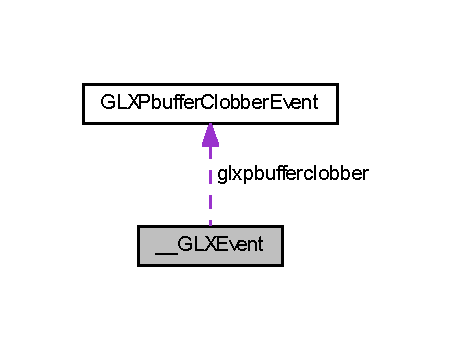
\includegraphics[width=217pt]{union_____g_l_x_event__coll__graph}
\end{center}
\end{figure}
\subsection*{Public Attributes}
\begin{DoxyCompactItemize}
\item 
\hypertarget{union_____g_l_x_event_ada5880e2b424bcb2f60a411aaf713fae}{\hyperlink{struct_g_l_x_pbuffer_clobber_event}{G\-L\-X\-Pbuffer\-Clobber\-Event} {\bfseries glxpbufferclobber}}\label{union_____g_l_x_event_ada5880e2b424bcb2f60a411aaf713fae}

\item 
\hypertarget{union_____g_l_x_event_a1cb8f6e7e77a34d25baf43b3f3bc2d4f}{long {\bfseries pad} \mbox{[}24\mbox{]}}\label{union_____g_l_x_event_a1cb8f6e7e77a34d25baf43b3f3bc2d4f}

\end{DoxyCompactItemize}


The documentation for this union was generated from the following file\-:\begin{DoxyCompactItemize}
\item 
glew-\/1.\-9.\-0/include/\-G\-L/glxew.\-h\end{DoxyCompactItemize}

\hypertarget{struct___g_p_u___d_e_v_i_c_e}{\section{\-\_\-\-G\-P\-U\-\_\-\-D\-E\-V\-I\-C\-E Struct Reference}
\label{struct___g_p_u___d_e_v_i_c_e}\index{\-\_\-\-G\-P\-U\-\_\-\-D\-E\-V\-I\-C\-E@{\-\_\-\-G\-P\-U\-\_\-\-D\-E\-V\-I\-C\-E}}
}
\subsection*{Public Attributes}
\begin{DoxyCompactItemize}
\item 
\hypertarget{struct___g_p_u___d_e_v_i_c_e_afcb22f16ba9e526610489ff56ab78ddb}{D\-W\-O\-R\-D {\bfseries cb}}\label{struct___g_p_u___d_e_v_i_c_e_afcb22f16ba9e526610489ff56ab78ddb}

\item 
\hypertarget{struct___g_p_u___d_e_v_i_c_e_a604bfab61f1a2c5d1e635837d369ba14}{C\-H\-A\-R {\bfseries Device\-Name} \mbox{[}32\mbox{]}}\label{struct___g_p_u___d_e_v_i_c_e_a604bfab61f1a2c5d1e635837d369ba14}

\item 
\hypertarget{struct___g_p_u___d_e_v_i_c_e_aff8b7920ccc85afcd6f325da6cdb0b73}{C\-H\-A\-R {\bfseries Device\-String} \mbox{[}128\mbox{]}}\label{struct___g_p_u___d_e_v_i_c_e_aff8b7920ccc85afcd6f325da6cdb0b73}

\item 
\hypertarget{struct___g_p_u___d_e_v_i_c_e_a008db9d0f5fc13a5160805f40465f14a}{D\-W\-O\-R\-D {\bfseries Flags}}\label{struct___g_p_u___d_e_v_i_c_e_a008db9d0f5fc13a5160805f40465f14a}

\item 
\hypertarget{struct___g_p_u___d_e_v_i_c_e_aeb573bbeb3b6c589246720ef259b9a27}{R\-E\-C\-T {\bfseries rc\-Virtual\-Screen}}\label{struct___g_p_u___d_e_v_i_c_e_aeb573bbeb3b6c589246720ef259b9a27}

\end{DoxyCompactItemize}


The documentation for this struct was generated from the following file\-:\begin{DoxyCompactItemize}
\item 
glew-\/1.\-9.\-0/include/\-G\-L/wglew.\-h\end{DoxyCompactItemize}

\hypertarget{class_base_property}{\section{Base\-Property Class Reference}
\label{class_base_property}\index{Base\-Property@{Base\-Property}}
}


Base property class.  




{\ttfamily \#include $<$baseproperty.\-h$>$}



Inheritance diagram for Base\-Property\-:
\nopagebreak
\begin{figure}[H]
\begin{center}
\leavevmode
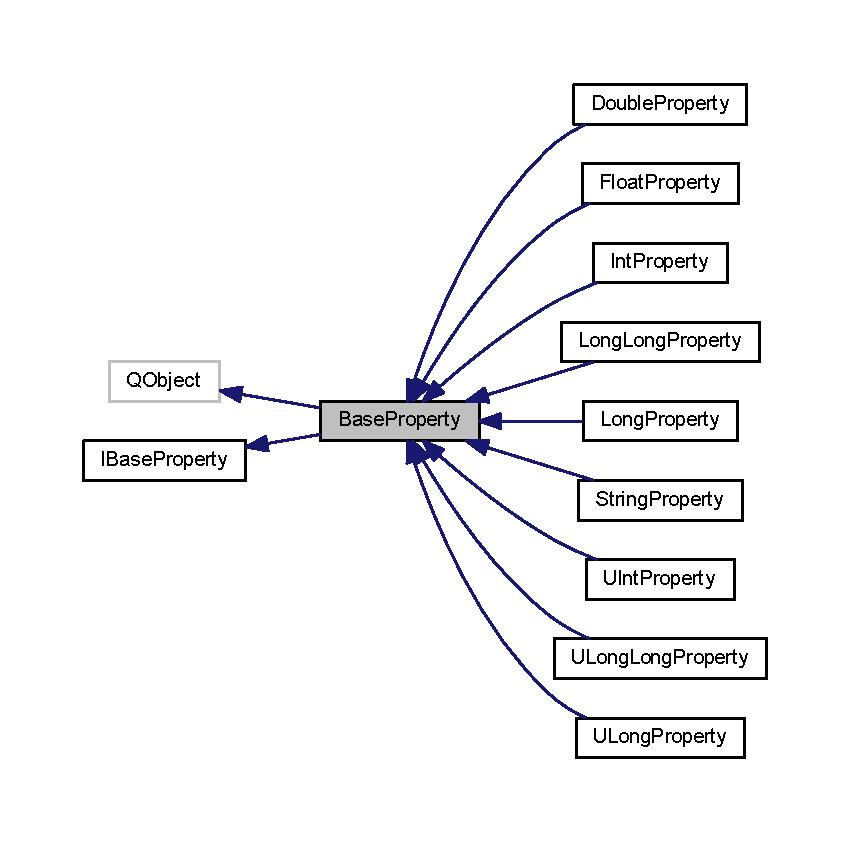
\includegraphics[width=350pt]{class_base_property__inherit__graph}
\end{center}
\end{figure}


Collaboration diagram for Base\-Property\-:
\nopagebreak
\begin{figure}[H]
\begin{center}
\leavevmode
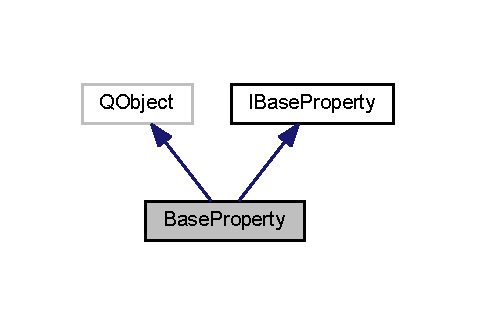
\includegraphics[width=229pt]{class_base_property__coll__graph}
\end{center}
\end{figure}
\subsection*{Public Member Functions}
\begin{DoxyCompactItemize}
\item 
\hyperlink{class_base_property_aca37cc72811875adbb8a5f5f91e521a2}{Base\-Property} (Q\-Object $\ast$parent=0, Q\-String key=\char`\"{}\char`\"{}, Q\-String value=\char`\"{}\char`\"{}, Q\-String comment=\char`\"{}\char`\"{})
\begin{DoxyCompactList}\small\item\em If key, value and comment are unspecified, they default to empty strings. \end{DoxyCompactList}\item 
\hyperlink{class_w_base_property}{W\-Base\-Property} $\ast$ \hyperlink{class_base_property_a032130dea4bd72ee8dd80dcfa7d5f37a}{slots\-Base} () const 
\begin{DoxyCompactList}\small\item\em Returns the interface wrapper to allow binding to slots on this property. \end{DoxyCompactList}\item 
virtual Q\-String \hyperlink{class_base_property_a7b5d5d1009130976d7a53720c6c8dab7}{get\-Key} () const 
\begin{DoxyCompactList}\small\item\em Returns the property key as a string. \end{DoxyCompactList}\item 
virtual Q\-String \hyperlink{class_base_property_a9656d6fa643734ae606fd613349e8f40}{get\-Value\-Raw} () const 
\begin{DoxyCompactList}\small\item\em Returns the property value as a raw string. \end{DoxyCompactList}\item 
virtual Q\-String \hyperlink{class_base_property_a77b2576711cabd4b4f0b39ae79868ebf}{get\-Comment} () const 
\begin{DoxyCompactList}\small\item\em Returns the comment value as a raw string (without \char`\"{}//\char`\"{}). \end{DoxyCompactList}\item 
virtual void \hyperlink{class_base_property_a5ed5f7ca81d54b1506e62ed23db2a8c5}{set\-Key} (Q\-String key)
\begin{DoxyCompactList}\small\item\em Sets the property key as a string. N\-O\-T\-E\-: Should be unique. \end{DoxyCompactList}\item 
virtual void \hyperlink{class_base_property_adf0d7a0e824a9d058387336d91514539}{set\-Value\-Raw} (Q\-String value)
\begin{DoxyCompactList}\small\item\em Sets the property value as a raw string, ignoring the intended property format. \end{DoxyCompactList}\item 
virtual void \hyperlink{class_base_property_ac882e4b94451ae00ab78d79afde84de5}{set\-Comment} (Q\-String value)
\begin{DoxyCompactList}\small\item\em Sets the comment value as a raw string (without \char`\"{}//\char`\"{}). \end{DoxyCompactList}\end{DoxyCompactItemize}
\subsection*{Protected Attributes}
\begin{DoxyCompactItemize}
\item 
Q\-Pair$<$ Q\-String, Q\-String $>$ \hyperlink{class_base_property_a2338fecdc198936259809444e93e93df}{m\-\_\-\-Property}
\item 
Q\-String \hyperlink{class_base_property_a2a08935cf352cb274575be32188e8acd}{m\-\_\-\-Comment}
\end{DoxyCompactItemize}


\subsection{Detailed Description}
Base property class. 

Base property class defining the basic property functions. Although this property deals with Q\-Strings only, a formal \hyperlink{class_string_property}{String\-Property} is available and recommended for use with strings. 

\subsection{Constructor \& Destructor Documentation}
\hypertarget{class_base_property_aca37cc72811875adbb8a5f5f91e521a2}{\index{Base\-Property@{Base\-Property}!Base\-Property@{Base\-Property}}
\index{Base\-Property@{Base\-Property}!BaseProperty@{Base\-Property}}
\subsubsection[{Base\-Property}]{\setlength{\rightskip}{0pt plus 5cm}Base\-Property\-::\-Base\-Property (
\begin{DoxyParamCaption}
\item[{Q\-Object $\ast$}]{parent = {\ttfamily 0}, }
\item[{Q\-String}]{key = {\ttfamily \char`\"{}\char`\"{}}, }
\item[{Q\-String}]{value = {\ttfamily \char`\"{}\char`\"{}}, }
\item[{Q\-String}]{comment = {\ttfamily \char`\"{}\char`\"{}}}
\end{DoxyParamCaption}
)\hspace{0.3cm}{\ttfamily [explicit]}}}\label{class_base_property_aca37cc72811875adbb8a5f5f91e521a2}


If key, value and comment are unspecified, they default to empty strings. 


\begin{DoxyParams}{Parameters}
{\em parent} & Parent object for this property. \\
\hline
{\em key} & Property key (should be unique). \\
\hline
{\em value} & Property value. \\
\hline
{\em comment} & Optional comment for if we are printing this property into a file. \\
\hline
\end{DoxyParams}


\subsection{Member Function Documentation}
\hypertarget{class_base_property_a77b2576711cabd4b4f0b39ae79868ebf}{\index{Base\-Property@{Base\-Property}!get\-Comment@{get\-Comment}}
\index{get\-Comment@{get\-Comment}!BaseProperty@{Base\-Property}}
\subsubsection[{get\-Comment}]{\setlength{\rightskip}{0pt plus 5cm}Q\-String Base\-Property\-::get\-Comment (
\begin{DoxyParamCaption}
{}
\end{DoxyParamCaption}
) const\hspace{0.3cm}{\ttfamily [inline]}, {\ttfamily [virtual]}}}\label{class_base_property_a77b2576711cabd4b4f0b39ae79868ebf}


Returns the comment value as a raw string (without \char`\"{}//\char`\"{}). 

\begin{DoxyReturn}{Returns}
Unformatted comment string. 
\end{DoxyReturn}


Implements \hyperlink{class_i_base_property_a53f9fd81c8247dfce1ac651576dd4119}{I\-Base\-Property}.

\hypertarget{class_base_property_a7b5d5d1009130976d7a53720c6c8dab7}{\index{Base\-Property@{Base\-Property}!get\-Key@{get\-Key}}
\index{get\-Key@{get\-Key}!BaseProperty@{Base\-Property}}
\subsubsection[{get\-Key}]{\setlength{\rightskip}{0pt plus 5cm}Q\-String Base\-Property\-::get\-Key (
\begin{DoxyParamCaption}
{}
\end{DoxyParamCaption}
) const\hspace{0.3cm}{\ttfamily [inline]}, {\ttfamily [virtual]}}}\label{class_base_property_a7b5d5d1009130976d7a53720c6c8dab7}


Returns the property key as a string. 

\begin{DoxyReturn}{Returns}
Q\-String representing the property's key. 
\end{DoxyReturn}


Implements \hyperlink{class_i_base_property_acbec936e956aa7fe59737af25e8b1962}{I\-Base\-Property}.

\hypertarget{class_base_property_a9656d6fa643734ae606fd613349e8f40}{\index{Base\-Property@{Base\-Property}!get\-Value\-Raw@{get\-Value\-Raw}}
\index{get\-Value\-Raw@{get\-Value\-Raw}!BaseProperty@{Base\-Property}}
\subsubsection[{get\-Value\-Raw}]{\setlength{\rightskip}{0pt plus 5cm}Q\-String Base\-Property\-::get\-Value\-Raw (
\begin{DoxyParamCaption}
{}
\end{DoxyParamCaption}
) const\hspace{0.3cm}{\ttfamily [inline]}, {\ttfamily [virtual]}}}\label{class_base_property_a9656d6fa643734ae606fd613349e8f40}


Returns the property value as a raw string. 

\begin{DoxyReturn}{Returns}
Q\-String representation of the value the property holds. 
\end{DoxyReturn}


Implements \hyperlink{class_i_base_property_adf7edb55057975980bac6b6fc5514d15}{I\-Base\-Property}.

\hypertarget{class_base_property_ac882e4b94451ae00ab78d79afde84de5}{\index{Base\-Property@{Base\-Property}!set\-Comment@{set\-Comment}}
\index{set\-Comment@{set\-Comment}!BaseProperty@{Base\-Property}}
\subsubsection[{set\-Comment}]{\setlength{\rightskip}{0pt plus 5cm}void Base\-Property\-::set\-Comment (
\begin{DoxyParamCaption}
\item[{Q\-String}]{value}
\end{DoxyParamCaption}
)\hspace{0.3cm}{\ttfamily [inline]}, {\ttfamily [virtual]}}}\label{class_base_property_ac882e4b94451ae00ab78d79afde84de5}


Sets the comment value as a raw string (without \char`\"{}//\char`\"{}). 


\begin{DoxyParams}{Parameters}
{\em value} & Comment string to set. \\
\hline
\end{DoxyParams}


Implements \hyperlink{class_i_base_property_ac749532ada813980bcb0a2f74ec45460}{I\-Base\-Property}.

\hypertarget{class_base_property_a5ed5f7ca81d54b1506e62ed23db2a8c5}{\index{Base\-Property@{Base\-Property}!set\-Key@{set\-Key}}
\index{set\-Key@{set\-Key}!BaseProperty@{Base\-Property}}
\subsubsection[{set\-Key}]{\setlength{\rightskip}{0pt plus 5cm}void Base\-Property\-::set\-Key (
\begin{DoxyParamCaption}
\item[{Q\-String}]{key}
\end{DoxyParamCaption}
)\hspace{0.3cm}{\ttfamily [inline]}, {\ttfamily [virtual]}}}\label{class_base_property_a5ed5f7ca81d54b1506e62ed23db2a8c5}


Sets the property key as a string. N\-O\-T\-E\-: Should be unique. 


\begin{DoxyParams}{Parameters}
{\em key} & The key to set. \\
\hline
\end{DoxyParams}


Implements \hyperlink{class_i_base_property_ad30bd2bc99dee7717390adccb8156c9b}{I\-Base\-Property}.

\hypertarget{class_base_property_adf0d7a0e824a9d058387336d91514539}{\index{Base\-Property@{Base\-Property}!set\-Value\-Raw@{set\-Value\-Raw}}
\index{set\-Value\-Raw@{set\-Value\-Raw}!BaseProperty@{Base\-Property}}
\subsubsection[{set\-Value\-Raw}]{\setlength{\rightskip}{0pt plus 5cm}void Base\-Property\-::set\-Value\-Raw (
\begin{DoxyParamCaption}
\item[{Q\-String}]{value}
\end{DoxyParamCaption}
)\hspace{0.3cm}{\ttfamily [inline]}, {\ttfamily [virtual]}}}\label{class_base_property_adf0d7a0e824a9d058387336d91514539}


Sets the property value as a raw string, ignoring the intended property format. 


\begin{DoxyParams}{Parameters}
{\em value} & String value to set. \\
\hline
\end{DoxyParams}


Implements \hyperlink{class_i_base_property_a39895fa933cddf290aeab127ba9aaa94}{I\-Base\-Property}.

\hypertarget{class_base_property_a032130dea4bd72ee8dd80dcfa7d5f37a}{\index{Base\-Property@{Base\-Property}!slots\-Base@{slots\-Base}}
\index{slots\-Base@{slots\-Base}!BaseProperty@{Base\-Property}}
\subsubsection[{slots\-Base}]{\setlength{\rightskip}{0pt plus 5cm}{\bf W\-Base\-Property}$\ast$ Base\-Property\-::slots\-Base (
\begin{DoxyParamCaption}
{}
\end{DoxyParamCaption}
) const\hspace{0.3cm}{\ttfamily [inline]}}}\label{class_base_property_a032130dea4bd72ee8dd80dcfa7d5f37a}


Returns the interface wrapper to allow binding to slots on this property. 

\begin{DoxyReturn}{Returns}
\hyperlink{class_w_base_property}{W\-Base\-Property} interface wrapper. 
\end{DoxyReturn}


\subsection{Member Data Documentation}
\hypertarget{class_base_property_a2a08935cf352cb274575be32188e8acd}{\index{Base\-Property@{Base\-Property}!m\-\_\-\-Comment@{m\-\_\-\-Comment}}
\index{m\-\_\-\-Comment@{m\-\_\-\-Comment}!BaseProperty@{Base\-Property}}
\subsubsection[{m\-\_\-\-Comment}]{\setlength{\rightskip}{0pt plus 5cm}Q\-String Base\-Property\-::m\-\_\-\-Comment\hspace{0.3cm}{\ttfamily [protected]}}}\label{class_base_property_a2a08935cf352cb274575be32188e8acd}
Optional property comment. \hypertarget{class_base_property_a2338fecdc198936259809444e93e93df}{\index{Base\-Property@{Base\-Property}!m\-\_\-\-Property@{m\-\_\-\-Property}}
\index{m\-\_\-\-Property@{m\-\_\-\-Property}!BaseProperty@{Base\-Property}}
\subsubsection[{m\-\_\-\-Property}]{\setlength{\rightskip}{0pt plus 5cm}Q\-Pair$<$Q\-String, Q\-String$>$ Base\-Property\-::m\-\_\-\-Property\hspace{0.3cm}{\ttfamily [protected]}}}\label{class_base_property_a2338fecdc198936259809444e93e93df}
Property key and value. 

The documentation for this class was generated from the following files\-:\begin{DoxyCompactItemize}
\item 
app/\hyperlink{baseproperty_8h}{baseproperty.\-h}\item 
app/baseproperty.\-cpp\end{DoxyCompactItemize}

\hypertarget{class_command_line_parser}{\section{Command\-Line\-Parser Class Reference}
\label{class_command_line_parser}\index{Command\-Line\-Parser@{Command\-Line\-Parser}}
}


Deals with arguments passed to the application on the command-\/line.  




{\ttfamily \#include $<$commandlineparser.\-h$>$}



Inheritance diagram for Command\-Line\-Parser\-:
\nopagebreak
\begin{figure}[H]
\begin{center}
\leavevmode
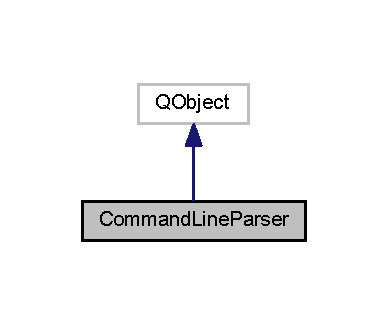
\includegraphics[width=186pt]{class_command_line_parser__inherit__graph}
\end{center}
\end{figure}


Collaboration diagram for Command\-Line\-Parser\-:
\nopagebreak
\begin{figure}[H]
\begin{center}
\leavevmode
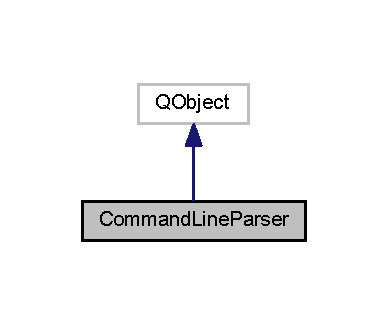
\includegraphics[width=186pt]{class_command_line_parser__coll__graph}
\end{center}
\end{figure}
\subsection*{Public Slots}
\begin{DoxyCompactItemize}
\item 
void \hyperlink{class_command_line_parser_a6a39c14ecf639b02bf8a71ac224b0a61}{Parse\-Arguments} (int argc, char $\ast$$\ast$argv)
\begin{DoxyCompactList}\small\item\em Parses the command-\/line arguments from the ignition function. \end{DoxyCompactList}\end{DoxyCompactItemize}
\subsection*{Public Member Functions}
\begin{DoxyCompactItemize}
\item 
\hyperlink{class_command_line_parser_af9c962bcd44ea242d11b88c9c28bd78d}{Command\-Line\-Parser} (Q\-Object $\ast$parent=0)
\begin{DoxyCompactList}\small\item\em Constructor. \end{DoxyCompactList}\item 
bool \hyperlink{class_command_line_parser_ac50e9de49d6e16174f6d5cf3f89c76d7}{Debugging} ()
\begin{DoxyCompactList}\small\item\em Is the application in debug mode? \end{DoxyCompactList}\item 
bool \hyperlink{class_command_line_parser_aaa2d8544c7841c33c560bb4410144154}{Logging} ()
\begin{DoxyCompactList}\small\item\em Is logging mode enabled? \end{DoxyCompactList}\end{DoxyCompactItemize}


\subsection{Detailed Description}
Deals with arguments passed to the application on the command-\/line. 

The command-\/line parser is created before the main application window is initialised and parses any options sent to the application on the command line. The global instance of the parser is made available through \hyperlink{globals_8h}{globals.\-h} under g\-\_\-p\-Cmd\-Line and several macros exist for facilitating the checking of common global application properties. See \hyperlink{globals_8h}{globals.\-h} for a full description. 

\subsection{Constructor \& Destructor Documentation}
\hypertarget{class_command_line_parser_af9c962bcd44ea242d11b88c9c28bd78d}{\index{Command\-Line\-Parser@{Command\-Line\-Parser}!Command\-Line\-Parser@{Command\-Line\-Parser}}
\index{Command\-Line\-Parser@{Command\-Line\-Parser}!CommandLineParser@{Command\-Line\-Parser}}
\subsubsection[{Command\-Line\-Parser}]{\setlength{\rightskip}{0pt plus 5cm}Command\-Line\-Parser\-::\-Command\-Line\-Parser (
\begin{DoxyParamCaption}
\item[{Q\-Object $\ast$}]{parent = {\ttfamily 0}}
\end{DoxyParamCaption}
)\hspace{0.3cm}{\ttfamily [explicit]}}}\label{class_command_line_parser_af9c962bcd44ea242d11b88c9c28bd78d}


Constructor. 


\begin{DoxyParams}{Parameters}
{\em parent} & Parent object (usually N\-U\-L\-L). \\
\hline
\end{DoxyParams}


\subsection{Member Function Documentation}
\hypertarget{class_command_line_parser_ac50e9de49d6e16174f6d5cf3f89c76d7}{\index{Command\-Line\-Parser@{Command\-Line\-Parser}!Debugging@{Debugging}}
\index{Debugging@{Debugging}!CommandLineParser@{Command\-Line\-Parser}}
\subsubsection[{Debugging}]{\setlength{\rightskip}{0pt plus 5cm}bool Command\-Line\-Parser\-::\-Debugging (
\begin{DoxyParamCaption}
{}
\end{DoxyParamCaption}
)}}\label{class_command_line_parser_ac50e9de49d6e16174f6d5cf3f89c76d7}


Is the application in debug mode? 

\begin{DoxyNote}{Note}
If enabled, the log window is available from the main application Debug menu.

If not specified, debugging mode defaults to false. 
\end{DoxyNote}
\begin{DoxyReturn}{Returns}
True if in debug mode, false otherwise. 
\end{DoxyReturn}
\hypertarget{class_command_line_parser_aaa2d8544c7841c33c560bb4410144154}{\index{Command\-Line\-Parser@{Command\-Line\-Parser}!Logging@{Logging}}
\index{Logging@{Logging}!CommandLineParser@{Command\-Line\-Parser}}
\subsubsection[{Logging}]{\setlength{\rightskip}{0pt plus 5cm}bool Command\-Line\-Parser\-::\-Logging (
\begin{DoxyParamCaption}
{}
\end{DoxyParamCaption}
)}}\label{class_command_line_parser_aaa2d8544c7841c33c560bb4410144154}


Is logging mode enabled? 

\begin{DoxyNote}{Note}
If enabled, logging messsages are written to a log file. If in debug mode, logging mode is also enabled.

If not specified, logging mode defaults to false. 
\end{DoxyNote}
\begin{DoxyReturn}{Returns}
True if enabled, false otherwise. 
\end{DoxyReturn}
\hypertarget{class_command_line_parser_a6a39c14ecf639b02bf8a71ac224b0a61}{\index{Command\-Line\-Parser@{Command\-Line\-Parser}!Parse\-Arguments@{Parse\-Arguments}}
\index{Parse\-Arguments@{Parse\-Arguments}!CommandLineParser@{Command\-Line\-Parser}}
\subsubsection[{Parse\-Arguments}]{\setlength{\rightskip}{0pt plus 5cm}void Command\-Line\-Parser\-::\-Parse\-Arguments (
\begin{DoxyParamCaption}
\item[{int}]{argc, }
\item[{char $\ast$$\ast$}]{argv}
\end{DoxyParamCaption}
)\hspace{0.3cm}{\ttfamily [slot]}}}\label{class_command_line_parser_a6a39c14ecf639b02bf8a71ac224b0a61}


Parses the command-\/line arguments from the ignition function. 


\begin{DoxyParams}{Parameters}
{\em argc} & Number of arguments. \\
\hline
{\em argv} & Char array of arguments. \\
\hline
\end{DoxyParams}


The documentation for this class was generated from the following files\-:\begin{DoxyCompactItemize}
\item 
app/\hyperlink{commandlineparser_8h}{commandlineparser.\-h}\item 
app/commandlineparser.\-cpp\end{DoxyCompactItemize}

\hypertarget{class_double_property}{\section{Double\-Property Class Reference}
\label{class_double_property}\index{Double\-Property@{Double\-Property}}
}


M\-A\-C\-R\-O P\-R\-O\-P\-E\-R\-T\-Y F\-O\-R double .  




{\ttfamily \#include $<$property.\-h$>$}



Inheritance diagram for Double\-Property\-:
\nopagebreak
\begin{figure}[H]
\begin{center}
\leavevmode
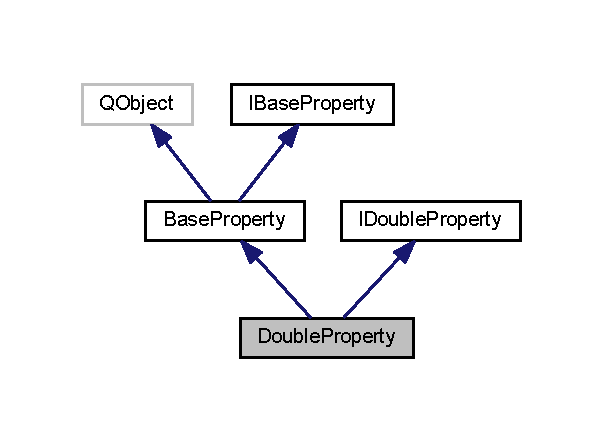
\includegraphics[width=290pt]{class_double_property__inherit__graph}
\end{center}
\end{figure}


Collaboration diagram for Double\-Property\-:
\nopagebreak
\begin{figure}[H]
\begin{center}
\leavevmode
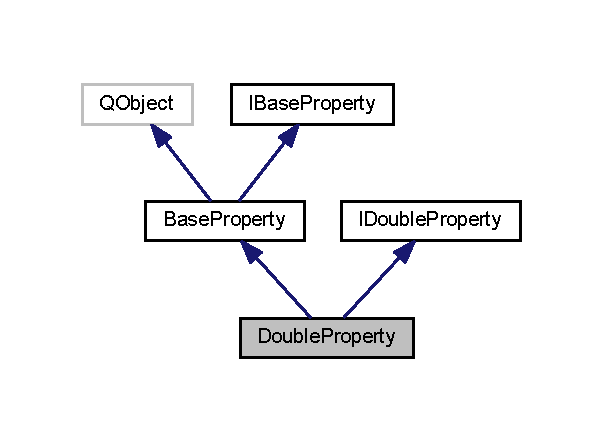
\includegraphics[width=290pt]{class_double_property__coll__graph}
\end{center}
\end{figure}
\subsection*{Public Member Functions}
\begin{DoxyCompactItemize}
\item 
\hyperlink{class_double_property_ad6db31eafe29ec0337a91b297b5648fa}{Double\-Property} (Q\-Object $\ast$parent=0, Q\-String key=\char`\"{}\char`\"{}, double value=0.\-0, Q\-String comment=\char`\"{}\char`\"{})
\begin{DoxyCompactList}\small\item\em Constructor. Parameters not passed are initialised to safe null values. \end{DoxyCompactList}\item 
virtual \hyperlink{group___property_classes_ga38f1ccddda12c7cb50b868c9f789ee37}{Property\-\_\-t} \hyperlink{class_double_property_a161c45cff47e246a6d27133562af064d}{get\-Property\-Type} () const 
\begin{DoxyCompactList}\small\item\em Returns the Property\-\_\-t to classify this property. \end{DoxyCompactList}\item 
virtual bool \hyperlink{class_double_property_a1c82626c933039cb28619e3723f16e6c}{pass\-To} (\hyperlink{class_property_variant}{Property\-Variant} $\ast$variant)
\begin{DoxyCompactList}\small\item\em Passes the property's value to the variant. \end{DoxyCompactList}\item 
virtual double \hyperlink{class_double_property_a9e196465f85c5fba581dc207dfd60eee}{get\-Value} (bool $\ast$success) const 
\begin{DoxyCompactList}\small\item\em Gets this property's value as double . \end{DoxyCompactList}\item 
virtual bool \hyperlink{class_double_property_a9ce3240555af31c5d4fbe9be33624637}{can\-Convert} () const 
\begin{DoxyCompactList}\small\item\em Returns whether or not the property's value can be successfully converted. \end{DoxyCompactList}\item 
virtual void \hyperlink{class_double_property_a1ae2a71c28ab126ac5eeceffdcdf4226}{set\-Value} (double value)
\begin{DoxyCompactList}\small\item\em Sets the property's value as double . \end{DoxyCompactList}\item 
virtual \hyperlink{class_w_double_property}{W\-Double\-Property} $\ast$ \hyperlink{class_double_property_a383b82607989d0a1abfd778ed7b30803}{slots\-For} () const 
\begin{DoxyCompactList}\small\item\em Returns the interface wrapper to allow binding to slots on this property. \end{DoxyCompactList}\end{DoxyCompactItemize}
\subsection*{Additional Inherited Members}


\subsection{Detailed Description}
M\-A\-C\-R\-O P\-R\-O\-P\-E\-R\-T\-Y F\-O\-R double . 

Property that handles data of type double . 

\subsection{Constructor \& Destructor Documentation}
\hypertarget{class_double_property_ad6db31eafe29ec0337a91b297b5648fa}{\index{Double\-Property@{Double\-Property}!Double\-Property@{Double\-Property}}
\index{Double\-Property@{Double\-Property}!DoubleProperty@{Double\-Property}}
\subsubsection[{Double\-Property}]{\setlength{\rightskip}{0pt plus 5cm}Double\-Property\-::\-Double\-Property (
\begin{DoxyParamCaption}
\item[{Q\-Object $\ast$}]{parent = {\ttfamily 0}, }
\item[{Q\-String}]{key = {\ttfamily \char`\"{}\char`\"{}}, }
\item[{double}]{value = {\ttfamily 0.0}, }
\item[{Q\-String}]{comment = {\ttfamily \char`\"{}\char`\"{}}}
\end{DoxyParamCaption}
)\hspace{0.3cm}{\ttfamily [explicit]}}}\label{class_double_property_ad6db31eafe29ec0337a91b297b5648fa}


Constructor. Parameters not passed are initialised to safe null values. 


\begin{DoxyParams}{Parameters}
{\em parent} & Parent object for this property.\\
\hline
{\em key} & Property key (should be unique).\\
\hline
{\em value} & Property value of type double .\\
\hline
{\em comment} & Optional string comment for when this property is written into a config file. \\
\hline
\end{DoxyParams}


\subsection{Member Function Documentation}
\hypertarget{class_double_property_a9ce3240555af31c5d4fbe9be33624637}{\index{Double\-Property@{Double\-Property}!can\-Convert@{can\-Convert}}
\index{can\-Convert@{can\-Convert}!DoubleProperty@{Double\-Property}}
\subsubsection[{can\-Convert}]{\setlength{\rightskip}{0pt plus 5cm}bool Double\-Property\-::can\-Convert (
\begin{DoxyParamCaption}
{}
\end{DoxyParamCaption}
) const\hspace{0.3cm}{\ttfamily [virtual]}}}\label{class_double_property_a9ce3240555af31c5d4fbe9be33624637}


Returns whether or not the property's value can be successfully converted. 

\begin{DoxyReturn}{Returns}
True if conversion is possible, false otherwise. 
\end{DoxyReturn}


Implements \hyperlink{class_i_double_property_afe5368913e955ec08c2797521d43d24a}{I\-Double\-Property}.

\hypertarget{class_double_property_a161c45cff47e246a6d27133562af064d}{\index{Double\-Property@{Double\-Property}!get\-Property\-Type@{get\-Property\-Type}}
\index{get\-Property\-Type@{get\-Property\-Type}!DoubleProperty@{Double\-Property}}
\subsubsection[{get\-Property\-Type}]{\setlength{\rightskip}{0pt plus 5cm}virtual {\bf Property\-\_\-t} Double\-Property\-::get\-Property\-Type (
\begin{DoxyParamCaption}
{}
\end{DoxyParamCaption}
) const\hspace{0.3cm}{\ttfamily [inline]}, {\ttfamily [virtual]}}}\label{class_double_property_a161c45cff47e246a6d27133562af064d}


Returns the Property\-\_\-t to classify this property. 

\begin{DoxyReturn}{Returns}
Property\-\_\-t classifier. 
\end{DoxyReturn}


Reimplemented from \hyperlink{class_base_property_a85239fb7297edb01c3176e4ce1b11132}{Base\-Property}.

\hypertarget{class_double_property_a9e196465f85c5fba581dc207dfd60eee}{\index{Double\-Property@{Double\-Property}!get\-Value@{get\-Value}}
\index{get\-Value@{get\-Value}!DoubleProperty@{Double\-Property}}
\subsubsection[{get\-Value}]{\setlength{\rightskip}{0pt plus 5cm}double Double\-Property\-::get\-Value (
\begin{DoxyParamCaption}
\item[{bool $\ast$}]{success}
\end{DoxyParamCaption}
) const\hspace{0.3cm}{\ttfamily [virtual]}}}\label{class_double_property_a9e196465f85c5fba581dc207dfd60eee}


Gets this property's value as double . 


\begin{DoxyParams}{Parameters}
{\em success} & True if conversion was successful, false otherwise.\\
\hline
\end{DoxyParams}
\begin{DoxyReturn}{Returns}
The property's value. 
\end{DoxyReturn}


Implements \hyperlink{class_i_double_property_af9143d685793a22249eb50b2515260ac}{I\-Double\-Property}.

\hypertarget{class_double_property_a1c82626c933039cb28619e3723f16e6c}{\index{Double\-Property@{Double\-Property}!pass\-To@{pass\-To}}
\index{pass\-To@{pass\-To}!DoubleProperty@{Double\-Property}}
\subsubsection[{pass\-To}]{\setlength{\rightskip}{0pt plus 5cm}bool Double\-Property\-::pass\-To (
\begin{DoxyParamCaption}
\item[{{\bf Property\-Variant} $\ast$}]{variant}
\end{DoxyParamCaption}
)\hspace{0.3cm}{\ttfamily [virtual]}}}\label{class_double_property_a1c82626c933039cb28619e3723f16e6c}


Passes the property's value to the variant. 


\begin{DoxyParams}{Parameters}
{\em variant} & Variant to pass to.\\
\hline
\end{DoxyParams}
\begin{DoxyReturn}{Returns}
True if conversion succeeded, false otherwise.
\end{DoxyReturn}

\begin{DoxyParams}{Parameters}
{\em variant} & Variant to pass to. \\
\hline
\end{DoxyParams}


Implements \hyperlink{class_i_double_property_a84794c76ff8b48f676d9ca3fef8c22c5}{I\-Double\-Property}.

\hypertarget{class_double_property_a1ae2a71c28ab126ac5eeceffdcdf4226}{\index{Double\-Property@{Double\-Property}!set\-Value@{set\-Value}}
\index{set\-Value@{set\-Value}!DoubleProperty@{Double\-Property}}
\subsubsection[{set\-Value}]{\setlength{\rightskip}{0pt plus 5cm}void Double\-Property\-::set\-Value (
\begin{DoxyParamCaption}
\item[{double}]{value}
\end{DoxyParamCaption}
)\hspace{0.3cm}{\ttfamily [virtual]}}}\label{class_double_property_a1ae2a71c28ab126ac5eeceffdcdf4226}


Sets the property's value as double . 


\begin{DoxyParams}{Parameters}
{\em value} & Value to set. \\
\hline
\end{DoxyParams}


Implements \hyperlink{class_i_double_property_a900dcb23ea5981475417e3cdfee001e3}{I\-Double\-Property}.

\hypertarget{class_double_property_a383b82607989d0a1abfd778ed7b30803}{\index{Double\-Property@{Double\-Property}!slots\-For@{slots\-For}}
\index{slots\-For@{slots\-For}!DoubleProperty@{Double\-Property}}
\subsubsection[{slots\-For}]{\setlength{\rightskip}{0pt plus 5cm}virtual {\bf W\-Double\-Property}$\ast$ Double\-Property\-::slots\-For (
\begin{DoxyParamCaption}
{}
\end{DoxyParamCaption}
) const\hspace{0.3cm}{\ttfamily [inline]}, {\ttfamily [virtual]}}}\label{class_double_property_a383b82607989d0a1abfd778ed7b30803}


Returns the interface wrapper to allow binding to slots on this property. 

\begin{DoxyReturn}{Returns}
\hyperlink{class_w_double_property}{W\-Double\-Property} interface wrapper. 
\end{DoxyReturn}


The documentation for this class was generated from the following files\-:\begin{DoxyCompactItemize}
\item 
app/\hyperlink{property_8h}{property.\-h}\item 
app/property.\-cpp\end{DoxyCompactItemize}

\hypertarget{class_float_property}{\section{Float\-Property Class Reference}
\label{class_float_property}\index{Float\-Property@{Float\-Property}}
}


M\-A\-C\-R\-O P\-R\-O\-P\-E\-R\-T\-Y F\-O\-R float .  




{\ttfamily \#include $<$property.\-h$>$}



Inheritance diagram for Float\-Property\-:
\nopagebreak
\begin{figure}[H]
\begin{center}
\leavevmode
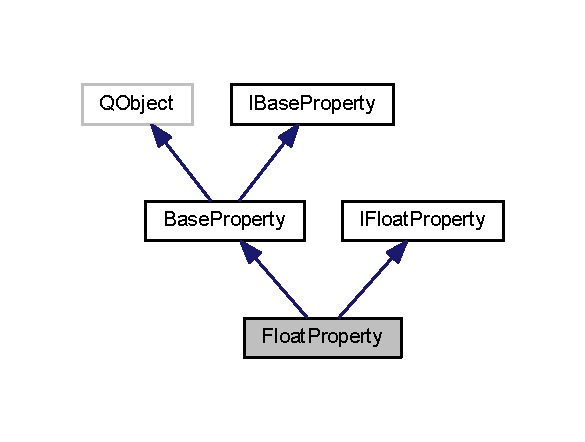
\includegraphics[width=281pt]{class_float_property__inherit__graph}
\end{center}
\end{figure}


Collaboration diagram for Float\-Property\-:
\nopagebreak
\begin{figure}[H]
\begin{center}
\leavevmode
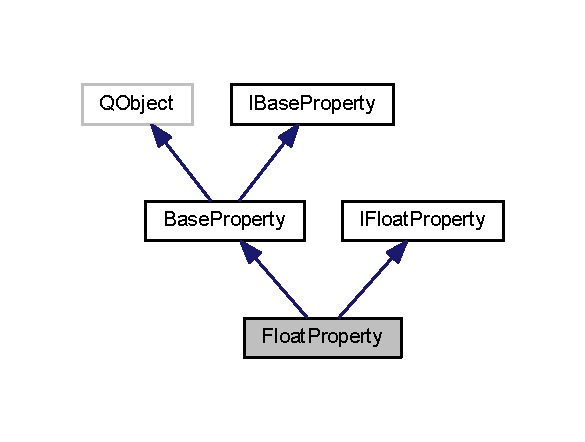
\includegraphics[width=281pt]{class_float_property__coll__graph}
\end{center}
\end{figure}
\subsection*{Public Member Functions}
\begin{DoxyCompactItemize}
\item 
\hyperlink{class_float_property_a94120bb05019e3cfc064b8ef7ab86e00}{Float\-Property} (Q\-Object $\ast$parent=0, Q\-String key=\char`\"{}\char`\"{}, float value=0.\-0, Q\-String comment=\char`\"{}\char`\"{})
\begin{DoxyCompactList}\small\item\em Constructor. Parameters not passed are initialised to safe null values. \end{DoxyCompactList}\item 
virtual \hyperlink{group___property_classes_ga38f1ccddda12c7cb50b868c9f789ee37}{Property\-\_\-t} \hyperlink{class_float_property_ac224ce3448cbe08d9c1b28804233086b}{get\-Property\-Type} () const 
\begin{DoxyCompactList}\small\item\em Returns the Property\-\_\-t to classify this property. \end{DoxyCompactList}\item 
virtual float \hyperlink{class_float_property_a91854af44926b14c2264d16d71c06f11}{get\-Value} (bool $\ast$success) const 
\begin{DoxyCompactList}\small\item\em Gets this property's value as float . \end{DoxyCompactList}\item 
virtual bool \hyperlink{class_float_property_a38c95c8f0a4131f5fd8a4a09352ba984}{can\-Convert} () const 
\begin{DoxyCompactList}\small\item\em Returns whether or not the property's value can be successfully converted. \end{DoxyCompactList}\item 
virtual void \hyperlink{class_float_property_a24ef985394b6273da923cf0165620568}{set\-Value} (float value)
\begin{DoxyCompactList}\small\item\em Sets the property's value as float . \end{DoxyCompactList}\item 
virtual \hyperlink{class_w_float_property}{W\-Float\-Property} $\ast$ \hyperlink{class_float_property_aa8f23ba9718273d96802b051d510b087}{slots\-For} () const 
\begin{DoxyCompactList}\small\item\em Returns the interface wrapper to allow binding to slots on this property. \end{DoxyCompactList}\end{DoxyCompactItemize}
\subsection*{Additional Inherited Members}


\subsection{Detailed Description}
M\-A\-C\-R\-O P\-R\-O\-P\-E\-R\-T\-Y F\-O\-R float . 

Property that handles data of type float . 

\subsection{Constructor \& Destructor Documentation}
\hypertarget{class_float_property_a94120bb05019e3cfc064b8ef7ab86e00}{\index{Float\-Property@{Float\-Property}!Float\-Property@{Float\-Property}}
\index{Float\-Property@{Float\-Property}!FloatProperty@{Float\-Property}}
\subsubsection[{Float\-Property}]{\setlength{\rightskip}{0pt plus 5cm}Float\-Property\-::\-Float\-Property (
\begin{DoxyParamCaption}
\item[{Q\-Object $\ast$}]{parent = {\ttfamily 0}, }
\item[{Q\-String}]{key = {\ttfamily \char`\"{}\char`\"{}}, }
\item[{float}]{value = {\ttfamily 0.0}, }
\item[{Q\-String}]{comment = {\ttfamily \char`\"{}\char`\"{}}}
\end{DoxyParamCaption}
)\hspace{0.3cm}{\ttfamily [explicit]}}}\label{class_float_property_a94120bb05019e3cfc064b8ef7ab86e00}


Constructor. Parameters not passed are initialised to safe null values. 


\begin{DoxyParams}{Parameters}
{\em parent} & Parent object for this property.\\
\hline
{\em key} & Property key (should be unique).\\
\hline
{\em value} & Property value of type float .\\
\hline
{\em comment} & Optional string comment for when this property is written into a config file. \\
\hline
\end{DoxyParams}


\subsection{Member Function Documentation}
\hypertarget{class_float_property_a38c95c8f0a4131f5fd8a4a09352ba984}{\index{Float\-Property@{Float\-Property}!can\-Convert@{can\-Convert}}
\index{can\-Convert@{can\-Convert}!FloatProperty@{Float\-Property}}
\subsubsection[{can\-Convert}]{\setlength{\rightskip}{0pt plus 5cm}bool Float\-Property\-::can\-Convert (
\begin{DoxyParamCaption}
{}
\end{DoxyParamCaption}
) const\hspace{0.3cm}{\ttfamily [virtual]}}}\label{class_float_property_a38c95c8f0a4131f5fd8a4a09352ba984}


Returns whether or not the property's value can be successfully converted. 

\begin{DoxyReturn}{Returns}
True if conversion is possible, false otherwise. 
\end{DoxyReturn}


Implements \hyperlink{class_i_float_property_a1e460fc2f90845794910bc74aabe5236}{I\-Float\-Property}.

\hypertarget{class_float_property_ac224ce3448cbe08d9c1b28804233086b}{\index{Float\-Property@{Float\-Property}!get\-Property\-Type@{get\-Property\-Type}}
\index{get\-Property\-Type@{get\-Property\-Type}!FloatProperty@{Float\-Property}}
\subsubsection[{get\-Property\-Type}]{\setlength{\rightskip}{0pt plus 5cm}virtual {\bf Property\-\_\-t} Float\-Property\-::get\-Property\-Type (
\begin{DoxyParamCaption}
{}
\end{DoxyParamCaption}
) const\hspace{0.3cm}{\ttfamily [inline]}, {\ttfamily [virtual]}}}\label{class_float_property_ac224ce3448cbe08d9c1b28804233086b}


Returns the Property\-\_\-t to classify this property. 

\begin{DoxyReturn}{Returns}
Property\-\_\-t classifier. 
\end{DoxyReturn}


Implements \hyperlink{class_i_float_property_a8d82006574891b63c2de22f9b49755a2}{I\-Float\-Property}.

\hypertarget{class_float_property_a91854af44926b14c2264d16d71c06f11}{\index{Float\-Property@{Float\-Property}!get\-Value@{get\-Value}}
\index{get\-Value@{get\-Value}!FloatProperty@{Float\-Property}}
\subsubsection[{get\-Value}]{\setlength{\rightskip}{0pt plus 5cm}float Float\-Property\-::get\-Value (
\begin{DoxyParamCaption}
\item[{bool $\ast$}]{success}
\end{DoxyParamCaption}
) const\hspace{0.3cm}{\ttfamily [virtual]}}}\label{class_float_property_a91854af44926b14c2264d16d71c06f11}


Gets this property's value as float . 


\begin{DoxyParams}{Parameters}
{\em success} & True if conversion was successful, false otherwise.\\
\hline
\end{DoxyParams}
\begin{DoxyReturn}{Returns}
The property's value. 
\end{DoxyReturn}


Implements \hyperlink{class_i_float_property_a5f3b98066c898de66db9141b01253d60}{I\-Float\-Property}.

\hypertarget{class_float_property_a24ef985394b6273da923cf0165620568}{\index{Float\-Property@{Float\-Property}!set\-Value@{set\-Value}}
\index{set\-Value@{set\-Value}!FloatProperty@{Float\-Property}}
\subsubsection[{set\-Value}]{\setlength{\rightskip}{0pt plus 5cm}void Float\-Property\-::set\-Value (
\begin{DoxyParamCaption}
\item[{float}]{value}
\end{DoxyParamCaption}
)\hspace{0.3cm}{\ttfamily [virtual]}}}\label{class_float_property_a24ef985394b6273da923cf0165620568}


Sets the property's value as float . 


\begin{DoxyParams}{Parameters}
{\em value} & Value to set. \\
\hline
\end{DoxyParams}


Implements \hyperlink{class_i_float_property_a358077ee2ced41069d9990d93ce5ddfa}{I\-Float\-Property}.

\hypertarget{class_float_property_aa8f23ba9718273d96802b051d510b087}{\index{Float\-Property@{Float\-Property}!slots\-For@{slots\-For}}
\index{slots\-For@{slots\-For}!FloatProperty@{Float\-Property}}
\subsubsection[{slots\-For}]{\setlength{\rightskip}{0pt plus 5cm}virtual {\bf W\-Float\-Property}$\ast$ Float\-Property\-::slots\-For (
\begin{DoxyParamCaption}
{}
\end{DoxyParamCaption}
) const\hspace{0.3cm}{\ttfamily [inline]}, {\ttfamily [virtual]}}}\label{class_float_property_aa8f23ba9718273d96802b051d510b087}


Returns the interface wrapper to allow binding to slots on this property. 

\begin{DoxyReturn}{Returns}
\hyperlink{class_w_float_property}{W\-Float\-Property} interface wrapper. 
\end{DoxyReturn}


The documentation for this class was generated from the following files\-:\begin{DoxyCompactItemize}
\item 
app/\hyperlink{property_8h}{property.\-h}\item 
app/property.\-cpp\end{DoxyCompactItemize}

\hypertarget{struct_g_l_x_buffer_clobber_event_s_g_i_x}{\section{G\-L\-X\-Buffer\-Clobber\-Event\-S\-G\-I\-X Struct Reference}
\label{struct_g_l_x_buffer_clobber_event_s_g_i_x}\index{G\-L\-X\-Buffer\-Clobber\-Event\-S\-G\-I\-X@{G\-L\-X\-Buffer\-Clobber\-Event\-S\-G\-I\-X}}
}
\subsection*{Public Attributes}
\begin{DoxyCompactItemize}
\item 
\hypertarget{struct_g_l_x_buffer_clobber_event_s_g_i_x_a36e3e8a5feea664623ea43d0f273b63a}{int {\bfseries type}}\label{struct_g_l_x_buffer_clobber_event_s_g_i_x_a36e3e8a5feea664623ea43d0f273b63a}

\item 
\hypertarget{struct_g_l_x_buffer_clobber_event_s_g_i_x_ac295e3276a7986eeae4d6a2a28c7e0b7}{unsigned long {\bfseries serial}}\label{struct_g_l_x_buffer_clobber_event_s_g_i_x_ac295e3276a7986eeae4d6a2a28c7e0b7}

\item 
\hypertarget{struct_g_l_x_buffer_clobber_event_s_g_i_x_af43bf0edbe40a74ef58dfb546a75118b}{Bool {\bfseries send\-\_\-event}}\label{struct_g_l_x_buffer_clobber_event_s_g_i_x_af43bf0edbe40a74ef58dfb546a75118b}

\item 
\hypertarget{struct_g_l_x_buffer_clobber_event_s_g_i_x_afef060d81026da75c846727f4a3de9d4}{Display $\ast$ {\bfseries display}}\label{struct_g_l_x_buffer_clobber_event_s_g_i_x_afef060d81026da75c846727f4a3de9d4}

\item 
\hypertarget{struct_g_l_x_buffer_clobber_event_s_g_i_x_a9c45674193ed80a79261c3b7518ee04f}{G\-L\-X\-Drawable {\bfseries drawable}}\label{struct_g_l_x_buffer_clobber_event_s_g_i_x_a9c45674193ed80a79261c3b7518ee04f}

\item 
\hypertarget{struct_g_l_x_buffer_clobber_event_s_g_i_x_a0b405123f1d6528f1f4dfa7ff92bde9b}{int {\bfseries event\-\_\-type}}\label{struct_g_l_x_buffer_clobber_event_s_g_i_x_a0b405123f1d6528f1f4dfa7ff92bde9b}

\item 
\hypertarget{struct_g_l_x_buffer_clobber_event_s_g_i_x_a25c31e8cbec0919f74a1e93ae74175b1}{int {\bfseries draw\-\_\-type}}\label{struct_g_l_x_buffer_clobber_event_s_g_i_x_a25c31e8cbec0919f74a1e93ae74175b1}

\item 
\hypertarget{struct_g_l_x_buffer_clobber_event_s_g_i_x_a74b4ad1ad3cac011001151411f621da1}{unsigned int {\bfseries mask}}\label{struct_g_l_x_buffer_clobber_event_s_g_i_x_a74b4ad1ad3cac011001151411f621da1}

\item 
\hypertarget{struct_g_l_x_buffer_clobber_event_s_g_i_x_a5118d48c3c8d5253d39922b5014b52ff}{int {\bfseries x}}\label{struct_g_l_x_buffer_clobber_event_s_g_i_x_a5118d48c3c8d5253d39922b5014b52ff}

\item 
\hypertarget{struct_g_l_x_buffer_clobber_event_s_g_i_x_aef21efa11558a5b67861f96471c56003}{int {\bfseries y}}\label{struct_g_l_x_buffer_clobber_event_s_g_i_x_aef21efa11558a5b67861f96471c56003}

\item 
\hypertarget{struct_g_l_x_buffer_clobber_event_s_g_i_x_adad23535733161528427584a42bfc6eb}{int {\bfseries width}}\label{struct_g_l_x_buffer_clobber_event_s_g_i_x_adad23535733161528427584a42bfc6eb}

\item 
\hypertarget{struct_g_l_x_buffer_clobber_event_s_g_i_x_a7838dbabb76c22aa8241310a3f2363ea}{int {\bfseries height}}\label{struct_g_l_x_buffer_clobber_event_s_g_i_x_a7838dbabb76c22aa8241310a3f2363ea}

\item 
\hypertarget{struct_g_l_x_buffer_clobber_event_s_g_i_x_ad8f4f0aae058e0a1ff542679823e37a9}{int {\bfseries count}}\label{struct_g_l_x_buffer_clobber_event_s_g_i_x_ad8f4f0aae058e0a1ff542679823e37a9}

\end{DoxyCompactItemize}


The documentation for this struct was generated from the following file\-:\begin{DoxyCompactItemize}
\item 
glew-\/1.\-9.\-0/include/\-G\-L/glxew.\-h\end{DoxyCompactItemize}

\hypertarget{struct_g_l_x_hyperpipe_config_s_g_i_x}{\section{G\-L\-X\-Hyperpipe\-Config\-S\-G\-I\-X Struct Reference}
\label{struct_g_l_x_hyperpipe_config_s_g_i_x}\index{G\-L\-X\-Hyperpipe\-Config\-S\-G\-I\-X@{G\-L\-X\-Hyperpipe\-Config\-S\-G\-I\-X}}
}
\subsection*{Public Attributes}
\begin{DoxyCompactItemize}
\item 
\hypertarget{struct_g_l_x_hyperpipe_config_s_g_i_x_a9e3748f92005cac81cb44d4c67acccb8}{char {\bfseries pipe\-Name} \mbox{[}G\-L\-X\-\_\-\-H\-Y\-P\-E\-R\-P\-I\-P\-E\-\_\-\-P\-I\-P\-E\-\_\-\-N\-A\-M\-E\-\_\-\-L\-E\-N\-G\-T\-H\-\_\-\-S\-G\-I\-X\mbox{]}}\label{struct_g_l_x_hyperpipe_config_s_g_i_x_a9e3748f92005cac81cb44d4c67acccb8}

\item 
\hypertarget{struct_g_l_x_hyperpipe_config_s_g_i_x_abc812d8796ba89d5de4e33b3532d8335}{int {\bfseries channel}}\label{struct_g_l_x_hyperpipe_config_s_g_i_x_abc812d8796ba89d5de4e33b3532d8335}

\item 
\hypertarget{struct_g_l_x_hyperpipe_config_s_g_i_x_a093cfaaec305531f66e1120929b5b01b}{unsigned int {\bfseries participation\-Type}}\label{struct_g_l_x_hyperpipe_config_s_g_i_x_a093cfaaec305531f66e1120929b5b01b}

\item 
\hypertarget{struct_g_l_x_hyperpipe_config_s_g_i_x_afe9288e75dc1ae5e0f33eff978d7024d}{int {\bfseries time\-Slice}}\label{struct_g_l_x_hyperpipe_config_s_g_i_x_afe9288e75dc1ae5e0f33eff978d7024d}

\end{DoxyCompactItemize}


The documentation for this struct was generated from the following file\-:\begin{DoxyCompactItemize}
\item 
glew-\/1.\-9.\-0/include/\-G\-L/glxew.\-h\end{DoxyCompactItemize}

\hypertarget{struct_g_l_x_hyperpipe_network_s_g_i_x}{\section{G\-L\-X\-Hyperpipe\-Network\-S\-G\-I\-X Struct Reference}
\label{struct_g_l_x_hyperpipe_network_s_g_i_x}\index{G\-L\-X\-Hyperpipe\-Network\-S\-G\-I\-X@{G\-L\-X\-Hyperpipe\-Network\-S\-G\-I\-X}}
}
\subsection*{Public Attributes}
\begin{DoxyCompactItemize}
\item 
\hypertarget{struct_g_l_x_hyperpipe_network_s_g_i_x_a6338b9717fa895aec16b932f2ef693ed}{char {\bfseries pipe\-Name} \mbox{[}G\-L\-X\-\_\-\-H\-Y\-P\-E\-R\-P\-I\-P\-E\-\_\-\-P\-I\-P\-E\-\_\-\-N\-A\-M\-E\-\_\-\-L\-E\-N\-G\-T\-H\-\_\-\-S\-G\-I\-X\mbox{]}}\label{struct_g_l_x_hyperpipe_network_s_g_i_x_a6338b9717fa895aec16b932f2ef693ed}

\item 
\hypertarget{struct_g_l_x_hyperpipe_network_s_g_i_x_a81393053988b32fadb0b21615024add1}{int {\bfseries network\-Id}}\label{struct_g_l_x_hyperpipe_network_s_g_i_x_a81393053988b32fadb0b21615024add1}

\end{DoxyCompactItemize}


The documentation for this struct was generated from the following file\-:\begin{DoxyCompactItemize}
\item 
glew-\/1.\-9.\-0/include/\-G\-L/glxew.\-h\end{DoxyCompactItemize}

\hypertarget{struct_g_l_x_pbuffer_clobber_event}{\section{G\-L\-X\-Pbuffer\-Clobber\-Event Struct Reference}
\label{struct_g_l_x_pbuffer_clobber_event}\index{G\-L\-X\-Pbuffer\-Clobber\-Event@{G\-L\-X\-Pbuffer\-Clobber\-Event}}
}
\subsection*{Public Attributes}
\begin{DoxyCompactItemize}
\item 
\hypertarget{struct_g_l_x_pbuffer_clobber_event_a30d7162d8d77246b01f5e610cda4da68}{int {\bfseries event\-\_\-type}}\label{struct_g_l_x_pbuffer_clobber_event_a30d7162d8d77246b01f5e610cda4da68}

\item 
\hypertarget{struct_g_l_x_pbuffer_clobber_event_a243f92b79d3cfbde73eab02815be2320}{int {\bfseries draw\-\_\-type}}\label{struct_g_l_x_pbuffer_clobber_event_a243f92b79d3cfbde73eab02815be2320}

\item 
\hypertarget{struct_g_l_x_pbuffer_clobber_event_a6390b2875ae06a4cb827d2b4c321eda3}{unsigned long {\bfseries serial}}\label{struct_g_l_x_pbuffer_clobber_event_a6390b2875ae06a4cb827d2b4c321eda3}

\item 
\hypertarget{struct_g_l_x_pbuffer_clobber_event_aa51969e67e4ad6095bda26ca64fe8ba6}{Bool {\bfseries send\-\_\-event}}\label{struct_g_l_x_pbuffer_clobber_event_aa51969e67e4ad6095bda26ca64fe8ba6}

\item 
\hypertarget{struct_g_l_x_pbuffer_clobber_event_aeb49bb93cc59448e75d66170a39596d1}{Display $\ast$ {\bfseries display}}\label{struct_g_l_x_pbuffer_clobber_event_aeb49bb93cc59448e75d66170a39596d1}

\item 
\hypertarget{struct_g_l_x_pbuffer_clobber_event_a388908b766e35205c1a461ea8b60439f}{G\-L\-X\-Drawable {\bfseries drawable}}\label{struct_g_l_x_pbuffer_clobber_event_a388908b766e35205c1a461ea8b60439f}

\item 
\hypertarget{struct_g_l_x_pbuffer_clobber_event_aff4c23d00f6dad98427f8d32a5f10580}{unsigned int {\bfseries buffer\-\_\-mask}}\label{struct_g_l_x_pbuffer_clobber_event_aff4c23d00f6dad98427f8d32a5f10580}

\item 
\hypertarget{struct_g_l_x_pbuffer_clobber_event_a13193b6e7e3e52b15f754fe91403b7ec}{unsigned int {\bfseries aux\-\_\-buffer}}\label{struct_g_l_x_pbuffer_clobber_event_a13193b6e7e3e52b15f754fe91403b7ec}

\item 
\hypertarget{struct_g_l_x_pbuffer_clobber_event_a8f0a7162a033c89ee94ce535580dbc32}{int {\bfseries x}}\label{struct_g_l_x_pbuffer_clobber_event_a8f0a7162a033c89ee94ce535580dbc32}

\item 
\hypertarget{struct_g_l_x_pbuffer_clobber_event_a69eb7ac60d36ac3ec4550ac206cfc61f}{int {\bfseries y}}\label{struct_g_l_x_pbuffer_clobber_event_a69eb7ac60d36ac3ec4550ac206cfc61f}

\item 
\hypertarget{struct_g_l_x_pbuffer_clobber_event_aaca375fecb872c73c60cd5d0bfc7c7a5}{int {\bfseries width}}\label{struct_g_l_x_pbuffer_clobber_event_aaca375fecb872c73c60cd5d0bfc7c7a5}

\item 
\hypertarget{struct_g_l_x_pbuffer_clobber_event_aed4e539c896bdad15217bf92c28f8520}{int {\bfseries height}}\label{struct_g_l_x_pbuffer_clobber_event_aed4e539c896bdad15217bf92c28f8520}

\item 
\hypertarget{struct_g_l_x_pbuffer_clobber_event_a61e9f6b31738464dca67f909fcacd298}{int {\bfseries count}}\label{struct_g_l_x_pbuffer_clobber_event_a61e9f6b31738464dca67f909fcacd298}

\end{DoxyCompactItemize}


The documentation for this struct was generated from the following file\-:\begin{DoxyCompactItemize}
\item 
glew-\/1.\-9.\-0/include/\-G\-L/glxew.\-h\end{DoxyCompactItemize}

\hypertarget{struct_g_l_x_pipe_rect}{\section{G\-L\-X\-Pipe\-Rect Struct Reference}
\label{struct_g_l_x_pipe_rect}\index{G\-L\-X\-Pipe\-Rect@{G\-L\-X\-Pipe\-Rect}}
}
\subsection*{Public Attributes}
\begin{DoxyCompactItemize}
\item 
\hypertarget{struct_g_l_x_pipe_rect_aa4c4f60e9647705ddefa10f95a37cb79}{char {\bfseries pipe\-Name} \mbox{[}G\-L\-X\-\_\-\-H\-Y\-P\-E\-R\-P\-I\-P\-E\-\_\-\-P\-I\-P\-E\-\_\-\-N\-A\-M\-E\-\_\-\-L\-E\-N\-G\-T\-H\-\_\-\-S\-G\-I\-X\mbox{]}}\label{struct_g_l_x_pipe_rect_aa4c4f60e9647705ddefa10f95a37cb79}

\item 
\hypertarget{struct_g_l_x_pipe_rect_a9df2313c01f75d149e64f2ff467bc266}{int {\bfseries src\-X\-Origin}}\label{struct_g_l_x_pipe_rect_a9df2313c01f75d149e64f2ff467bc266}

\item 
\hypertarget{struct_g_l_x_pipe_rect_a1f7316dff7050ab2ce9d3d37f8c5450e}{int {\bfseries src\-Y\-Origin}}\label{struct_g_l_x_pipe_rect_a1f7316dff7050ab2ce9d3d37f8c5450e}

\item 
\hypertarget{struct_g_l_x_pipe_rect_a2c6c180a4dabb71076366e06a1c7d0ef}{int {\bfseries src\-Width}}\label{struct_g_l_x_pipe_rect_a2c6c180a4dabb71076366e06a1c7d0ef}

\item 
\hypertarget{struct_g_l_x_pipe_rect_a35632524bce6bffa05f284a9b1c1b8ff}{int {\bfseries src\-Height}}\label{struct_g_l_x_pipe_rect_a35632524bce6bffa05f284a9b1c1b8ff}

\item 
\hypertarget{struct_g_l_x_pipe_rect_a8b7b941894ad3420326d7e9fa885bb71}{int {\bfseries dest\-X\-Origin}}\label{struct_g_l_x_pipe_rect_a8b7b941894ad3420326d7e9fa885bb71}

\item 
\hypertarget{struct_g_l_x_pipe_rect_aef7766b02ef07c20a11e89da5878b469}{int {\bfseries dest\-Y\-Origin}}\label{struct_g_l_x_pipe_rect_aef7766b02ef07c20a11e89da5878b469}

\item 
\hypertarget{struct_g_l_x_pipe_rect_a3c07991d2a8fb6e973eae834650b3dad}{int {\bfseries dest\-Width}}\label{struct_g_l_x_pipe_rect_a3c07991d2a8fb6e973eae834650b3dad}

\item 
\hypertarget{struct_g_l_x_pipe_rect_a858b0ea6642e451495aff35cfefbd083}{int {\bfseries dest\-Height}}\label{struct_g_l_x_pipe_rect_a858b0ea6642e451495aff35cfefbd083}

\end{DoxyCompactItemize}


The documentation for this struct was generated from the following file\-:\begin{DoxyCompactItemize}
\item 
glew-\/1.\-9.\-0/include/\-G\-L/glxew.\-h\end{DoxyCompactItemize}

\hypertarget{struct_g_l_x_pipe_rect_limits}{\section{G\-L\-X\-Pipe\-Rect\-Limits Struct Reference}
\label{struct_g_l_x_pipe_rect_limits}\index{G\-L\-X\-Pipe\-Rect\-Limits@{G\-L\-X\-Pipe\-Rect\-Limits}}
}
\subsection*{Public Attributes}
\begin{DoxyCompactItemize}
\item 
\hypertarget{struct_g_l_x_pipe_rect_limits_ae78b4b6656101bc841946733a5b6e5ce}{char {\bfseries pipe\-Name} \mbox{[}G\-L\-X\-\_\-\-H\-Y\-P\-E\-R\-P\-I\-P\-E\-\_\-\-P\-I\-P\-E\-\_\-\-N\-A\-M\-E\-\_\-\-L\-E\-N\-G\-T\-H\-\_\-\-S\-G\-I\-X\mbox{]}}\label{struct_g_l_x_pipe_rect_limits_ae78b4b6656101bc841946733a5b6e5ce}

\item 
\hypertarget{struct_g_l_x_pipe_rect_limits_a3e5a965059d9f5d2ca42acd35af5bb9b}{int {\bfseries X\-Origin}}\label{struct_g_l_x_pipe_rect_limits_a3e5a965059d9f5d2ca42acd35af5bb9b}

\item 
\hypertarget{struct_g_l_x_pipe_rect_limits_a50e06bcf0dae95854be7d93a515199e9}{int {\bfseries Y\-Origin}}\label{struct_g_l_x_pipe_rect_limits_a50e06bcf0dae95854be7d93a515199e9}

\item 
\hypertarget{struct_g_l_x_pipe_rect_limits_a27572e499c0d3280031c2ad8e387c0c1}{int {\bfseries max\-Height}}\label{struct_g_l_x_pipe_rect_limits_a27572e499c0d3280031c2ad8e387c0c1}

\item 
\hypertarget{struct_g_l_x_pipe_rect_limits_a8662c7a712b30620e25fc994adf337a1}{int {\bfseries max\-Width}}\label{struct_g_l_x_pipe_rect_limits_a8662c7a712b30620e25fc994adf337a1}

\end{DoxyCompactItemize}


The documentation for this struct was generated from the following file\-:\begin{DoxyCompactItemize}
\item 
glew-\/1.\-9.\-0/include/\-G\-L/glxew.\-h\end{DoxyCompactItemize}

\hypertarget{class_i_base_property}{\section{I\-Base\-Property Class Reference}
\label{class_i_base_property}\index{I\-Base\-Property@{I\-Base\-Property}}
}


Base property interface.  




{\ttfamily \#include $<$baseproperty.\-h$>$}



Inheritance diagram for I\-Base\-Property\-:
\nopagebreak
\begin{figure}[H]
\begin{center}
\leavevmode
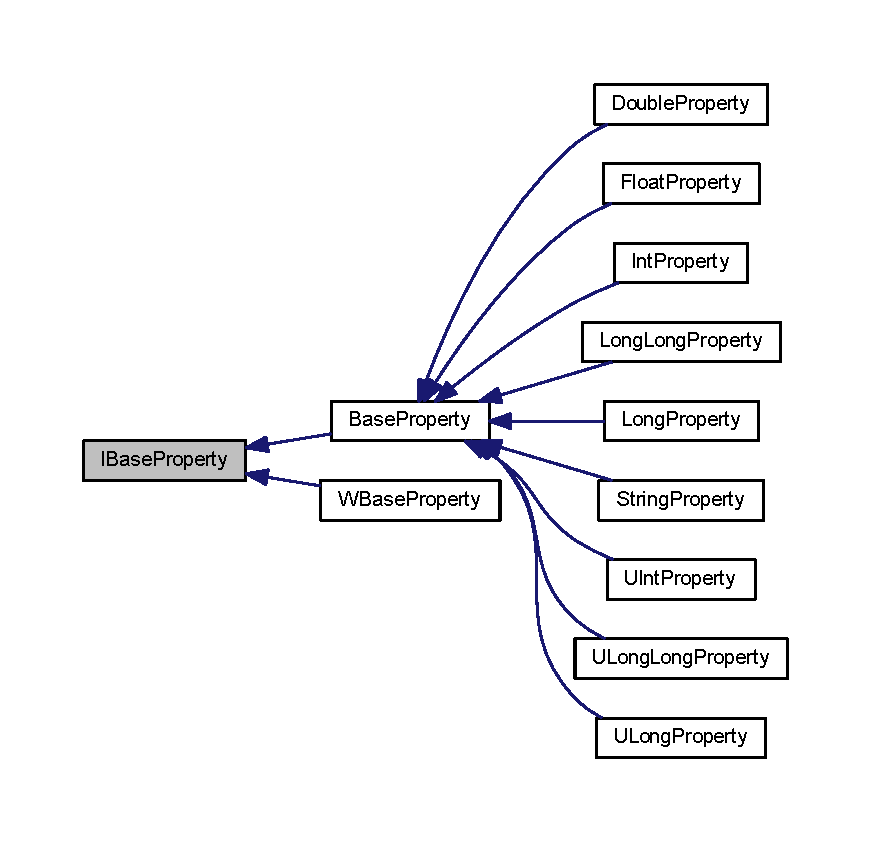
\includegraphics[width=350pt]{class_i_base_property__inherit__graph}
\end{center}
\end{figure}
\subsection*{Public Member Functions}
\begin{DoxyCompactItemize}
\item 
virtual Q\-String \hyperlink{class_i_base_property_acbec936e956aa7fe59737af25e8b1962}{get\-Key} () const =0
\begin{DoxyCompactList}\small\item\em Returns the property key as a string. \end{DoxyCompactList}\item 
virtual Q\-String \hyperlink{class_i_base_property_adf7edb55057975980bac6b6fc5514d15}{get\-Value\-Raw} () const =0
\begin{DoxyCompactList}\small\item\em Returns the property value as a raw string. \end{DoxyCompactList}\item 
virtual Q\-String \hyperlink{class_i_base_property_a53f9fd81c8247dfce1ac651576dd4119}{get\-Comment} () const =0
\begin{DoxyCompactList}\small\item\em Returns the comment value as a raw string (without \char`\"{}//\char`\"{}). \end{DoxyCompactList}\item 
virtual void \hyperlink{class_i_base_property_ad30bd2bc99dee7717390adccb8156c9b}{set\-Key} (Q\-String key)=0
\begin{DoxyCompactList}\small\item\em Sets the property key as a string. N\-O\-T\-E\-: Should be unique. \end{DoxyCompactList}\item 
virtual void \hyperlink{class_i_base_property_a39895fa933cddf290aeab127ba9aaa94}{set\-Value\-Raw} (Q\-String value)=0
\begin{DoxyCompactList}\small\item\em Sets the property value as a raw string, ignoring the intended property format. \end{DoxyCompactList}\item 
virtual void \hyperlink{class_i_base_property_ac749532ada813980bcb0a2f74ec45460}{set\-Comment} (Q\-String value)=0
\begin{DoxyCompactList}\small\item\em Sets the comment value as a raw string (without \char`\"{}//\char`\"{}). \end{DoxyCompactList}\end{DoxyCompactItemize}


\subsection{Detailed Description}
Base property interface. 

Implemented by \hyperlink{class_base_property}{Base\-Property}. To access slots, use \hyperlink{class_base_property_a032130dea4bd72ee8dd80dcfa7d5f37a}{Base\-Property\-::slots\-Base()}. 

\subsection{Member Function Documentation}
\hypertarget{class_i_base_property_a53f9fd81c8247dfce1ac651576dd4119}{\index{I\-Base\-Property@{I\-Base\-Property}!get\-Comment@{get\-Comment}}
\index{get\-Comment@{get\-Comment}!IBaseProperty@{I\-Base\-Property}}
\subsubsection[{get\-Comment}]{\setlength{\rightskip}{0pt plus 5cm}virtual Q\-String I\-Base\-Property\-::get\-Comment (
\begin{DoxyParamCaption}
{}
\end{DoxyParamCaption}
) const\hspace{0.3cm}{\ttfamily [pure virtual]}}}\label{class_i_base_property_a53f9fd81c8247dfce1ac651576dd4119}


Returns the comment value as a raw string (without \char`\"{}//\char`\"{}). 

\begin{DoxyReturn}{Returns}
Unformatted comment string. 
\end{DoxyReturn}


Implemented in \hyperlink{class_base_property_a77b2576711cabd4b4f0b39ae79868ebf}{Base\-Property}, and \hyperlink{class_w_base_property_a60750f9c78b6cbd7ec3fc1bfa9ae53fe}{W\-Base\-Property}.

\hypertarget{class_i_base_property_acbec936e956aa7fe59737af25e8b1962}{\index{I\-Base\-Property@{I\-Base\-Property}!get\-Key@{get\-Key}}
\index{get\-Key@{get\-Key}!IBaseProperty@{I\-Base\-Property}}
\subsubsection[{get\-Key}]{\setlength{\rightskip}{0pt plus 5cm}virtual Q\-String I\-Base\-Property\-::get\-Key (
\begin{DoxyParamCaption}
{}
\end{DoxyParamCaption}
) const\hspace{0.3cm}{\ttfamily [pure virtual]}}}\label{class_i_base_property_acbec936e956aa7fe59737af25e8b1962}


Returns the property key as a string. 

\begin{DoxyReturn}{Returns}
Q\-String representing the property's key. 
\end{DoxyReturn}


Implemented in \hyperlink{class_base_property_a7b5d5d1009130976d7a53720c6c8dab7}{Base\-Property}, and \hyperlink{class_w_base_property_a4c0e55c7b0a19a7685b30a985b72524a}{W\-Base\-Property}.

\hypertarget{class_i_base_property_adf7edb55057975980bac6b6fc5514d15}{\index{I\-Base\-Property@{I\-Base\-Property}!get\-Value\-Raw@{get\-Value\-Raw}}
\index{get\-Value\-Raw@{get\-Value\-Raw}!IBaseProperty@{I\-Base\-Property}}
\subsubsection[{get\-Value\-Raw}]{\setlength{\rightskip}{0pt plus 5cm}virtual Q\-String I\-Base\-Property\-::get\-Value\-Raw (
\begin{DoxyParamCaption}
{}
\end{DoxyParamCaption}
) const\hspace{0.3cm}{\ttfamily [pure virtual]}}}\label{class_i_base_property_adf7edb55057975980bac6b6fc5514d15}


Returns the property value as a raw string. 

\begin{DoxyReturn}{Returns}
Q\-String representation of the value the property holds. 
\end{DoxyReturn}


Implemented in \hyperlink{class_base_property_a9656d6fa643734ae606fd613349e8f40}{Base\-Property}, and \hyperlink{class_w_base_property_a49ba3186114cd7a0bb730a1a703af1eb}{W\-Base\-Property}.

\hypertarget{class_i_base_property_ac749532ada813980bcb0a2f74ec45460}{\index{I\-Base\-Property@{I\-Base\-Property}!set\-Comment@{set\-Comment}}
\index{set\-Comment@{set\-Comment}!IBaseProperty@{I\-Base\-Property}}
\subsubsection[{set\-Comment}]{\setlength{\rightskip}{0pt plus 5cm}virtual void I\-Base\-Property\-::set\-Comment (
\begin{DoxyParamCaption}
\item[{Q\-String}]{value}
\end{DoxyParamCaption}
)\hspace{0.3cm}{\ttfamily [pure virtual]}}}\label{class_i_base_property_ac749532ada813980bcb0a2f74ec45460}


Sets the comment value as a raw string (without \char`\"{}//\char`\"{}). 


\begin{DoxyParams}{Parameters}
{\em value} & Comment string to set. \\
\hline
\end{DoxyParams}


Implemented in \hyperlink{class_base_property_ac882e4b94451ae00ab78d79afde84de5}{Base\-Property}.

\hypertarget{class_i_base_property_ad30bd2bc99dee7717390adccb8156c9b}{\index{I\-Base\-Property@{I\-Base\-Property}!set\-Key@{set\-Key}}
\index{set\-Key@{set\-Key}!IBaseProperty@{I\-Base\-Property}}
\subsubsection[{set\-Key}]{\setlength{\rightskip}{0pt plus 5cm}virtual void I\-Base\-Property\-::set\-Key (
\begin{DoxyParamCaption}
\item[{Q\-String}]{key}
\end{DoxyParamCaption}
)\hspace{0.3cm}{\ttfamily [pure virtual]}}}\label{class_i_base_property_ad30bd2bc99dee7717390adccb8156c9b}


Sets the property key as a string. N\-O\-T\-E\-: Should be unique. 


\begin{DoxyParams}{Parameters}
{\em key} & The key to set. \\
\hline
\end{DoxyParams}


Implemented in \hyperlink{class_base_property_a5ed5f7ca81d54b1506e62ed23db2a8c5}{Base\-Property}.

\hypertarget{class_i_base_property_a39895fa933cddf290aeab127ba9aaa94}{\index{I\-Base\-Property@{I\-Base\-Property}!set\-Value\-Raw@{set\-Value\-Raw}}
\index{set\-Value\-Raw@{set\-Value\-Raw}!IBaseProperty@{I\-Base\-Property}}
\subsubsection[{set\-Value\-Raw}]{\setlength{\rightskip}{0pt plus 5cm}virtual void I\-Base\-Property\-::set\-Value\-Raw (
\begin{DoxyParamCaption}
\item[{Q\-String}]{value}
\end{DoxyParamCaption}
)\hspace{0.3cm}{\ttfamily [pure virtual]}}}\label{class_i_base_property_a39895fa933cddf290aeab127ba9aaa94}


Sets the property value as a raw string, ignoring the intended property format. 


\begin{DoxyParams}{Parameters}
{\em value} & String value to set. \\
\hline
\end{DoxyParams}


Implemented in \hyperlink{class_base_property_adf0d7a0e824a9d058387336d91514539}{Base\-Property}.



The documentation for this class was generated from the following file\-:\begin{DoxyCompactItemize}
\item 
app/\hyperlink{baseproperty_8h}{baseproperty.\-h}\end{DoxyCompactItemize}

\hypertarget{class_i_double_property}{\section{I\-Double\-Property Class Reference}
\label{class_i_double_property}\index{I\-Double\-Property@{I\-Double\-Property}}
}


M\-A\-C\-R\-O P\-R\-O\-P\-E\-R\-T\-Y I\-N\-T\-E\-R\-F\-A\-C\-E F\-O\-R double .  




{\ttfamily \#include $<$property.\-h$>$}



Inheritance diagram for I\-Double\-Property\-:
\nopagebreak
\begin{figure}[H]
\begin{center}
\leavevmode
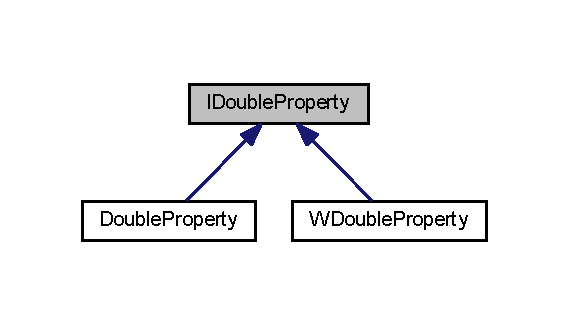
\includegraphics[width=273pt]{class_i_double_property__inherit__graph}
\end{center}
\end{figure}
\subsection*{Public Member Functions}
\begin{DoxyCompactItemize}
\item 
virtual double \hyperlink{class_i_double_property_af9143d685793a22249eb50b2515260ac}{get\-Value} (bool $\ast$success) const =0
\begin{DoxyCompactList}\small\item\em Gets this property's value as double . \end{DoxyCompactList}\item 
virtual void \hyperlink{class_i_double_property_a900dcb23ea5981475417e3cdfee001e3}{set\-Value} (double value)=0
\begin{DoxyCompactList}\small\item\em Sets the property's value as double . \end{DoxyCompactList}\item 
virtual bool \hyperlink{class_i_double_property_afe5368913e955ec08c2797521d43d24a}{can\-Convert} () const =0
\begin{DoxyCompactList}\small\item\em Returns whether or not the property's value can be successfully converted. \end{DoxyCompactList}\item 
virtual bool \hyperlink{class_i_double_property_a84794c76ff8b48f676d9ca3fef8c22c5}{pass\-To} (\hyperlink{class_property_variant}{Property\-Variant} $\ast$variant)=0
\begin{DoxyCompactList}\small\item\em Passes the property's value to the variant. \end{DoxyCompactList}\end{DoxyCompactItemize}


\subsection{Detailed Description}
M\-A\-C\-R\-O P\-R\-O\-P\-E\-R\-T\-Y I\-N\-T\-E\-R\-F\-A\-C\-E F\-O\-R double . 

Interface for property that handles data of type double . 

\subsection{Member Function Documentation}
\hypertarget{class_i_double_property_afe5368913e955ec08c2797521d43d24a}{\index{I\-Double\-Property@{I\-Double\-Property}!can\-Convert@{can\-Convert}}
\index{can\-Convert@{can\-Convert}!IDoubleProperty@{I\-Double\-Property}}
\subsubsection[{can\-Convert}]{\setlength{\rightskip}{0pt plus 5cm}virtual bool I\-Double\-Property\-::can\-Convert (
\begin{DoxyParamCaption}
{}
\end{DoxyParamCaption}
) const\hspace{0.3cm}{\ttfamily [pure virtual]}}}\label{class_i_double_property_afe5368913e955ec08c2797521d43d24a}


Returns whether or not the property's value can be successfully converted. 

\begin{DoxyReturn}{Returns}
True if conversion is possible, false otherwise. 
\end{DoxyReturn}


Implemented in \hyperlink{class_double_property_a9ce3240555af31c5d4fbe9be33624637}{Double\-Property}, and \hyperlink{class_w_double_property_acf72db76ced6c2dc50027bc2714be73b}{W\-Double\-Property}.

\hypertarget{class_i_double_property_af9143d685793a22249eb50b2515260ac}{\index{I\-Double\-Property@{I\-Double\-Property}!get\-Value@{get\-Value}}
\index{get\-Value@{get\-Value}!IDoubleProperty@{I\-Double\-Property}}
\subsubsection[{get\-Value}]{\setlength{\rightskip}{0pt plus 5cm}virtual double I\-Double\-Property\-::get\-Value (
\begin{DoxyParamCaption}
\item[{bool $\ast$}]{success}
\end{DoxyParamCaption}
) const\hspace{0.3cm}{\ttfamily [pure virtual]}}}\label{class_i_double_property_af9143d685793a22249eb50b2515260ac}


Gets this property's value as double . 


\begin{DoxyParams}{Parameters}
{\em success} & True if conversion was successful, false otherwise.\\
\hline
\end{DoxyParams}
\begin{DoxyReturn}{Returns}
The property's value. 
\end{DoxyReturn}


Implemented in \hyperlink{class_double_property_a9e196465f85c5fba581dc207dfd60eee}{Double\-Property}, and \hyperlink{class_w_double_property_ac771c45522b2682056081700effc7930}{W\-Double\-Property}.

\hypertarget{class_i_double_property_a84794c76ff8b48f676d9ca3fef8c22c5}{\index{I\-Double\-Property@{I\-Double\-Property}!pass\-To@{pass\-To}}
\index{pass\-To@{pass\-To}!IDoubleProperty@{I\-Double\-Property}}
\subsubsection[{pass\-To}]{\setlength{\rightskip}{0pt plus 5cm}virtual bool I\-Double\-Property\-::pass\-To (
\begin{DoxyParamCaption}
\item[{{\bf Property\-Variant} $\ast$}]{variant}
\end{DoxyParamCaption}
)\hspace{0.3cm}{\ttfamily [pure virtual]}}}\label{class_i_double_property_a84794c76ff8b48f676d9ca3fef8c22c5}


Passes the property's value to the variant. 


\begin{DoxyParams}{Parameters}
{\em variant} & Variant to pass to.\\
\hline
\end{DoxyParams}
\begin{DoxyReturn}{Returns}
True if conversion succeeded, false otherwise. 
\end{DoxyReturn}


Implemented in \hyperlink{class_double_property_a1c82626c933039cb28619e3723f16e6c}{Double\-Property}.

\hypertarget{class_i_double_property_a900dcb23ea5981475417e3cdfee001e3}{\index{I\-Double\-Property@{I\-Double\-Property}!set\-Value@{set\-Value}}
\index{set\-Value@{set\-Value}!IDoubleProperty@{I\-Double\-Property}}
\subsubsection[{set\-Value}]{\setlength{\rightskip}{0pt plus 5cm}virtual void I\-Double\-Property\-::set\-Value (
\begin{DoxyParamCaption}
\item[{double}]{value}
\end{DoxyParamCaption}
)\hspace{0.3cm}{\ttfamily [pure virtual]}}}\label{class_i_double_property_a900dcb23ea5981475417e3cdfee001e3}


Sets the property's value as double . 


\begin{DoxyParams}{Parameters}
{\em value} & Value to set. \\
\hline
\end{DoxyParams}


Implemented in \hyperlink{class_double_property_a1ae2a71c28ab126ac5eeceffdcdf4226}{Double\-Property}.



The documentation for this class was generated from the following file\-:\begin{DoxyCompactItemize}
\item 
app/\hyperlink{property_8h}{property.\-h}\end{DoxyCompactItemize}

\hypertarget{class_i_float_property}{\section{I\-Float\-Property Class Reference}
\label{class_i_float_property}\index{I\-Float\-Property@{I\-Float\-Property}}
}


M\-A\-C\-R\-O P\-R\-O\-P\-E\-R\-T\-Y I\-N\-T\-E\-R\-F\-A\-C\-E F\-O\-R float .  




{\ttfamily \#include $<$property.\-h$>$}



Inheritance diagram for I\-Float\-Property\-:
\nopagebreak
\begin{figure}[H]
\begin{center}
\leavevmode
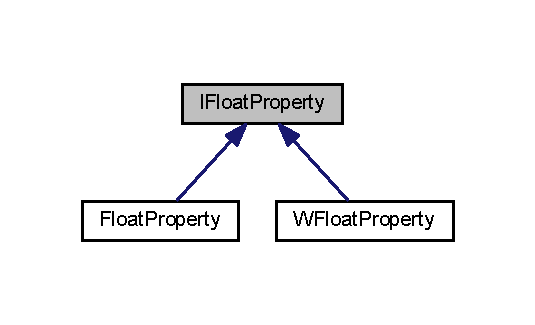
\includegraphics[width=257pt]{class_i_float_property__inherit__graph}
\end{center}
\end{figure}
\subsection*{Public Member Functions}
\begin{DoxyCompactItemize}
\item 
virtual float \hyperlink{class_i_float_property_a5f3b98066c898de66db9141b01253d60}{get\-Value} (bool $\ast$success) const =0
\begin{DoxyCompactList}\small\item\em Gets this property's value as float . \end{DoxyCompactList}\item 
virtual void \hyperlink{class_i_float_property_a358077ee2ced41069d9990d93ce5ddfa}{set\-Value} (float value)=0
\begin{DoxyCompactList}\small\item\em Sets the property's value as float . \end{DoxyCompactList}\item 
virtual bool \hyperlink{class_i_float_property_a1e460fc2f90845794910bc74aabe5236}{can\-Convert} () const =0
\begin{DoxyCompactList}\small\item\em Returns whether or not the property's value can be successfully converted. \end{DoxyCompactList}\item 
virtual bool \hyperlink{class_i_float_property_ab2c6d31035b4a5385545740a337be706}{pass\-To} (\hyperlink{class_property_variant}{Property\-Variant} $\ast$variant)=0
\begin{DoxyCompactList}\small\item\em Passes the property's value to the variant. \end{DoxyCompactList}\end{DoxyCompactItemize}


\subsection{Detailed Description}
M\-A\-C\-R\-O P\-R\-O\-P\-E\-R\-T\-Y I\-N\-T\-E\-R\-F\-A\-C\-E F\-O\-R float . 

Interface for property that handles data of type float . 

\subsection{Member Function Documentation}
\hypertarget{class_i_float_property_a1e460fc2f90845794910bc74aabe5236}{\index{I\-Float\-Property@{I\-Float\-Property}!can\-Convert@{can\-Convert}}
\index{can\-Convert@{can\-Convert}!IFloatProperty@{I\-Float\-Property}}
\subsubsection[{can\-Convert}]{\setlength{\rightskip}{0pt plus 5cm}virtual bool I\-Float\-Property\-::can\-Convert (
\begin{DoxyParamCaption}
{}
\end{DoxyParamCaption}
) const\hspace{0.3cm}{\ttfamily [pure virtual]}}}\label{class_i_float_property_a1e460fc2f90845794910bc74aabe5236}


Returns whether or not the property's value can be successfully converted. 

\begin{DoxyReturn}{Returns}
True if conversion is possible, false otherwise. 
\end{DoxyReturn}


Implemented in \hyperlink{class_float_property_a38c95c8f0a4131f5fd8a4a09352ba984}{Float\-Property}, and \hyperlink{class_w_float_property_a7eee2964a782c7909b11f7621504fc11}{W\-Float\-Property}.

\hypertarget{class_i_float_property_a5f3b98066c898de66db9141b01253d60}{\index{I\-Float\-Property@{I\-Float\-Property}!get\-Value@{get\-Value}}
\index{get\-Value@{get\-Value}!IFloatProperty@{I\-Float\-Property}}
\subsubsection[{get\-Value}]{\setlength{\rightskip}{0pt plus 5cm}virtual float I\-Float\-Property\-::get\-Value (
\begin{DoxyParamCaption}
\item[{bool $\ast$}]{success}
\end{DoxyParamCaption}
) const\hspace{0.3cm}{\ttfamily [pure virtual]}}}\label{class_i_float_property_a5f3b98066c898de66db9141b01253d60}


Gets this property's value as float . 


\begin{DoxyParams}{Parameters}
{\em success} & True if conversion was successful, false otherwise.\\
\hline
\end{DoxyParams}
\begin{DoxyReturn}{Returns}
The property's value. 
\end{DoxyReturn}


Implemented in \hyperlink{class_float_property_a91854af44926b14c2264d16d71c06f11}{Float\-Property}, and \hyperlink{class_w_float_property_acdfaccfb44bff32042d5eecb377f406d}{W\-Float\-Property}.

\hypertarget{class_i_float_property_ab2c6d31035b4a5385545740a337be706}{\index{I\-Float\-Property@{I\-Float\-Property}!pass\-To@{pass\-To}}
\index{pass\-To@{pass\-To}!IFloatProperty@{I\-Float\-Property}}
\subsubsection[{pass\-To}]{\setlength{\rightskip}{0pt plus 5cm}virtual bool I\-Float\-Property\-::pass\-To (
\begin{DoxyParamCaption}
\item[{{\bf Property\-Variant} $\ast$}]{variant}
\end{DoxyParamCaption}
)\hspace{0.3cm}{\ttfamily [pure virtual]}}}\label{class_i_float_property_ab2c6d31035b4a5385545740a337be706}


Passes the property's value to the variant. 


\begin{DoxyParams}{Parameters}
{\em variant} & Variant to pass to.\\
\hline
\end{DoxyParams}
\begin{DoxyReturn}{Returns}
True if conversion succeeded, false otherwise. 
\end{DoxyReturn}


Implemented in \hyperlink{class_float_property_a811c6ebe512a45d4fba73cbfd486c8f6}{Float\-Property}.

\hypertarget{class_i_float_property_a358077ee2ced41069d9990d93ce5ddfa}{\index{I\-Float\-Property@{I\-Float\-Property}!set\-Value@{set\-Value}}
\index{set\-Value@{set\-Value}!IFloatProperty@{I\-Float\-Property}}
\subsubsection[{set\-Value}]{\setlength{\rightskip}{0pt plus 5cm}virtual void I\-Float\-Property\-::set\-Value (
\begin{DoxyParamCaption}
\item[{float}]{value}
\end{DoxyParamCaption}
)\hspace{0.3cm}{\ttfamily [pure virtual]}}}\label{class_i_float_property_a358077ee2ced41069d9990d93ce5ddfa}


Sets the property's value as float . 


\begin{DoxyParams}{Parameters}
{\em value} & Value to set. \\
\hline
\end{DoxyParams}


Implemented in \hyperlink{class_float_property_a24ef985394b6273da923cf0165620568}{Float\-Property}.



The documentation for this class was generated from the following file\-:\begin{DoxyCompactItemize}
\item 
app/\hyperlink{property_8h}{property.\-h}\end{DoxyCompactItemize}

\hypertarget{class_i_int_property}{\section{I\-Int\-Property Class Reference}
\label{class_i_int_property}\index{I\-Int\-Property@{I\-Int\-Property}}
}


M\-A\-C\-R\-O P\-R\-O\-P\-E\-R\-T\-Y I\-N\-T\-E\-R\-F\-A\-C\-E F\-O\-R int .  




{\ttfamily \#include $<$property.\-h$>$}



Inheritance diagram for I\-Int\-Property\-:
\nopagebreak
\begin{figure}[H]
\begin{center}
\leavevmode
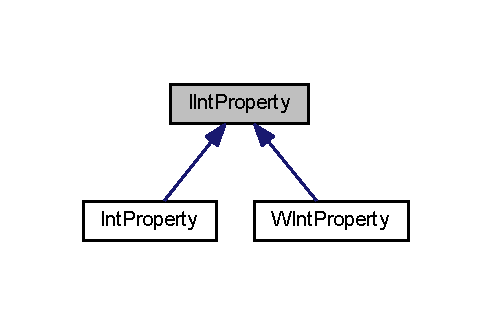
\includegraphics[width=236pt]{class_i_int_property__inherit__graph}
\end{center}
\end{figure}
\subsection*{Public Member Functions}
\begin{DoxyCompactItemize}
\item 
virtual int \hyperlink{class_i_int_property_a32bd5be46bee5c4a53180498767f51d0}{get\-Value} (bool $\ast$success) const =0
\begin{DoxyCompactList}\small\item\em Gets this property's value as int . \end{DoxyCompactList}\item 
virtual void \hyperlink{class_i_int_property_a6ba40997660af79851cbeaff5180e61d}{set\-Value} (int value)=0
\begin{DoxyCompactList}\small\item\em Sets the property's value as int . \end{DoxyCompactList}\item 
virtual bool \hyperlink{class_i_int_property_a25375f7c817ab7a1aeaef72a5bcfafdd}{can\-Convert} () const =0
\begin{DoxyCompactList}\small\item\em Returns whether or not the property's value can be successfully converted. \end{DoxyCompactList}\item 
virtual bool \hyperlink{class_i_int_property_a687991633f9155591842ac627cbc80f9}{pass\-To} (\hyperlink{class_property_variant}{Property\-Variant} $\ast$variant)=0
\begin{DoxyCompactList}\small\item\em Passes the property's value to the variant. \end{DoxyCompactList}\end{DoxyCompactItemize}


\subsection{Detailed Description}
M\-A\-C\-R\-O P\-R\-O\-P\-E\-R\-T\-Y I\-N\-T\-E\-R\-F\-A\-C\-E F\-O\-R int . 

Interface for property that handles data of type int . 

\subsection{Member Function Documentation}
\hypertarget{class_i_int_property_a25375f7c817ab7a1aeaef72a5bcfafdd}{\index{I\-Int\-Property@{I\-Int\-Property}!can\-Convert@{can\-Convert}}
\index{can\-Convert@{can\-Convert}!IIntProperty@{I\-Int\-Property}}
\subsubsection[{can\-Convert}]{\setlength{\rightskip}{0pt plus 5cm}virtual bool I\-Int\-Property\-::can\-Convert (
\begin{DoxyParamCaption}
{}
\end{DoxyParamCaption}
) const\hspace{0.3cm}{\ttfamily [pure virtual]}}}\label{class_i_int_property_a25375f7c817ab7a1aeaef72a5bcfafdd}


Returns whether or not the property's value can be successfully converted. 

\begin{DoxyReturn}{Returns}
True if conversion is possible, false otherwise. 
\end{DoxyReturn}


Implemented in \hyperlink{class_int_property_a3ce0216893c32bae0bb469fe1f82f83c}{Int\-Property}, and \hyperlink{class_w_int_property_a2aadf339189421871abccd98b553ce6b}{W\-Int\-Property}.

\hypertarget{class_i_int_property_a32bd5be46bee5c4a53180498767f51d0}{\index{I\-Int\-Property@{I\-Int\-Property}!get\-Value@{get\-Value}}
\index{get\-Value@{get\-Value}!IIntProperty@{I\-Int\-Property}}
\subsubsection[{get\-Value}]{\setlength{\rightskip}{0pt plus 5cm}virtual int I\-Int\-Property\-::get\-Value (
\begin{DoxyParamCaption}
\item[{bool $\ast$}]{success}
\end{DoxyParamCaption}
) const\hspace{0.3cm}{\ttfamily [pure virtual]}}}\label{class_i_int_property_a32bd5be46bee5c4a53180498767f51d0}


Gets this property's value as int . 


\begin{DoxyParams}{Parameters}
{\em success} & True if conversion was successful, false otherwise.\\
\hline
\end{DoxyParams}
\begin{DoxyReturn}{Returns}
The property's value. 
\end{DoxyReturn}


Implemented in \hyperlink{class_int_property_a721123bb68dd46f0d0247012b663d4ba}{Int\-Property}, and \hyperlink{class_w_int_property_aea678a96a398024ac3cdcdb31e5999de}{W\-Int\-Property}.

\hypertarget{class_i_int_property_a687991633f9155591842ac627cbc80f9}{\index{I\-Int\-Property@{I\-Int\-Property}!pass\-To@{pass\-To}}
\index{pass\-To@{pass\-To}!IIntProperty@{I\-Int\-Property}}
\subsubsection[{pass\-To}]{\setlength{\rightskip}{0pt plus 5cm}virtual bool I\-Int\-Property\-::pass\-To (
\begin{DoxyParamCaption}
\item[{{\bf Property\-Variant} $\ast$}]{variant}
\end{DoxyParamCaption}
)\hspace{0.3cm}{\ttfamily [pure virtual]}}}\label{class_i_int_property_a687991633f9155591842ac627cbc80f9}


Passes the property's value to the variant. 


\begin{DoxyParams}{Parameters}
{\em variant} & Variant to pass to.\\
\hline
\end{DoxyParams}
\begin{DoxyReturn}{Returns}
True if conversion succeeded, false otherwise. 
\end{DoxyReturn}


Implemented in \hyperlink{class_int_property_af7c54a340e388a667f68b6ddbec68f6e}{Int\-Property}.

\hypertarget{class_i_int_property_a6ba40997660af79851cbeaff5180e61d}{\index{I\-Int\-Property@{I\-Int\-Property}!set\-Value@{set\-Value}}
\index{set\-Value@{set\-Value}!IIntProperty@{I\-Int\-Property}}
\subsubsection[{set\-Value}]{\setlength{\rightskip}{0pt plus 5cm}virtual void I\-Int\-Property\-::set\-Value (
\begin{DoxyParamCaption}
\item[{int}]{value}
\end{DoxyParamCaption}
)\hspace{0.3cm}{\ttfamily [pure virtual]}}}\label{class_i_int_property_a6ba40997660af79851cbeaff5180e61d}


Sets the property's value as int . 


\begin{DoxyParams}{Parameters}
{\em value} & Value to set. \\
\hline
\end{DoxyParams}


Implemented in \hyperlink{class_int_property_a9c3b7ced3c8b7d8fbb9f739449e5622e}{Int\-Property}.



The documentation for this class was generated from the following file\-:\begin{DoxyCompactItemize}
\item 
app/\hyperlink{property_8h}{property.\-h}\end{DoxyCompactItemize}

\hypertarget{class_i_long_long_property}{\section{I\-Long\-Long\-Property Class Reference}
\label{class_i_long_long_property}\index{I\-Long\-Long\-Property@{I\-Long\-Long\-Property}}
}


M\-A\-C\-R\-O P\-R\-O\-P\-E\-R\-T\-Y I\-N\-T\-E\-R\-F\-A\-C\-E F\-O\-R qlonglong .  




{\ttfamily \#include $<$property.\-h$>$}



Inheritance diagram for I\-Long\-Long\-Property\-:
\nopagebreak
\begin{figure}[H]
\begin{center}
\leavevmode
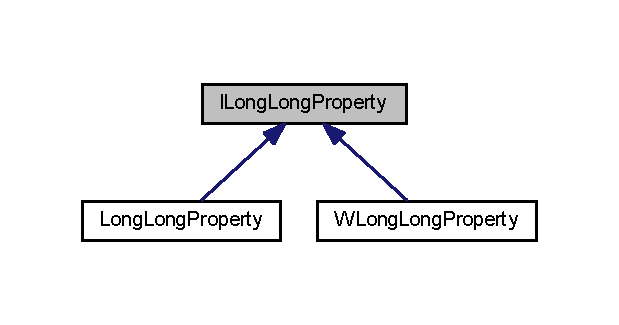
\includegraphics[width=297pt]{class_i_long_long_property__inherit__graph}
\end{center}
\end{figure}
\subsection*{Public Member Functions}
\begin{DoxyCompactItemize}
\item 
virtual qlonglong \hyperlink{class_i_long_long_property_a4364152258a2b085fa660ae34d106fdf}{get\-Value} (bool $\ast$success) const =0
\begin{DoxyCompactList}\small\item\em Gets this property's value as qlonglong . \end{DoxyCompactList}\item 
virtual void \hyperlink{class_i_long_long_property_a3ef096db3b5d53b1566148d9c78fcbbf}{set\-Value} (qlonglong value)=0
\begin{DoxyCompactList}\small\item\em Sets the property's value as qlonglong . \end{DoxyCompactList}\item 
virtual bool \hyperlink{class_i_long_long_property_a878b7753e3c53e966f9be8a3bd1e9b38}{can\-Convert} () const =0
\begin{DoxyCompactList}\small\item\em Returns whether or not the property's value can be successfully converted. \end{DoxyCompactList}\item 
virtual bool \hyperlink{class_i_long_long_property_a9134d0a324de1abf93ccd1bb866f06ad}{pass\-To} (\hyperlink{class_property_variant}{Property\-Variant} $\ast$variant)=0
\begin{DoxyCompactList}\small\item\em Passes the property's value to the variant. \end{DoxyCompactList}\end{DoxyCompactItemize}


\subsection{Detailed Description}
M\-A\-C\-R\-O P\-R\-O\-P\-E\-R\-T\-Y I\-N\-T\-E\-R\-F\-A\-C\-E F\-O\-R qlonglong . 

Interface for property that handles data of type qlonglong . 

\subsection{Member Function Documentation}
\hypertarget{class_i_long_long_property_a878b7753e3c53e966f9be8a3bd1e9b38}{\index{I\-Long\-Long\-Property@{I\-Long\-Long\-Property}!can\-Convert@{can\-Convert}}
\index{can\-Convert@{can\-Convert}!ILongLongProperty@{I\-Long\-Long\-Property}}
\subsubsection[{can\-Convert}]{\setlength{\rightskip}{0pt plus 5cm}virtual bool I\-Long\-Long\-Property\-::can\-Convert (
\begin{DoxyParamCaption}
{}
\end{DoxyParamCaption}
) const\hspace{0.3cm}{\ttfamily [pure virtual]}}}\label{class_i_long_long_property_a878b7753e3c53e966f9be8a3bd1e9b38}


Returns whether or not the property's value can be successfully converted. 

\begin{DoxyReturn}{Returns}
True if conversion is possible, false otherwise. 
\end{DoxyReturn}


Implemented in \hyperlink{class_long_long_property_a2690f56d6b804d37eec1457250da4acb}{Long\-Long\-Property}, and \hyperlink{class_w_long_long_property_a5b553e3d82d48cb661ef6180fa8ed76e}{W\-Long\-Long\-Property}.

\hypertarget{class_i_long_long_property_a4364152258a2b085fa660ae34d106fdf}{\index{I\-Long\-Long\-Property@{I\-Long\-Long\-Property}!get\-Value@{get\-Value}}
\index{get\-Value@{get\-Value}!ILongLongProperty@{I\-Long\-Long\-Property}}
\subsubsection[{get\-Value}]{\setlength{\rightskip}{0pt plus 5cm}virtual qlonglong I\-Long\-Long\-Property\-::get\-Value (
\begin{DoxyParamCaption}
\item[{bool $\ast$}]{success}
\end{DoxyParamCaption}
) const\hspace{0.3cm}{\ttfamily [pure virtual]}}}\label{class_i_long_long_property_a4364152258a2b085fa660ae34d106fdf}


Gets this property's value as qlonglong . 


\begin{DoxyParams}{Parameters}
{\em success} & True if conversion was successful, false otherwise.\\
\hline
\end{DoxyParams}
\begin{DoxyReturn}{Returns}
The property's value. 
\end{DoxyReturn}


Implemented in \hyperlink{class_long_long_property_a55da84c1e1c5db5431a3b5ddae6a72eb}{Long\-Long\-Property}, and \hyperlink{class_w_long_long_property_abae79b01d411ec7f44aa2d93289ad63f}{W\-Long\-Long\-Property}.

\hypertarget{class_i_long_long_property_a9134d0a324de1abf93ccd1bb866f06ad}{\index{I\-Long\-Long\-Property@{I\-Long\-Long\-Property}!pass\-To@{pass\-To}}
\index{pass\-To@{pass\-To}!ILongLongProperty@{I\-Long\-Long\-Property}}
\subsubsection[{pass\-To}]{\setlength{\rightskip}{0pt plus 5cm}virtual bool I\-Long\-Long\-Property\-::pass\-To (
\begin{DoxyParamCaption}
\item[{{\bf Property\-Variant} $\ast$}]{variant}
\end{DoxyParamCaption}
)\hspace{0.3cm}{\ttfamily [pure virtual]}}}\label{class_i_long_long_property_a9134d0a324de1abf93ccd1bb866f06ad}


Passes the property's value to the variant. 


\begin{DoxyParams}{Parameters}
{\em variant} & Variant to pass to.\\
\hline
\end{DoxyParams}
\begin{DoxyReturn}{Returns}
True if conversion succeeded, false otherwise. 
\end{DoxyReturn}


Implemented in \hyperlink{class_long_long_property_a4954cdf7702dcefc7e072934b2b4e80c}{Long\-Long\-Property}.

\hypertarget{class_i_long_long_property_a3ef096db3b5d53b1566148d9c78fcbbf}{\index{I\-Long\-Long\-Property@{I\-Long\-Long\-Property}!set\-Value@{set\-Value}}
\index{set\-Value@{set\-Value}!ILongLongProperty@{I\-Long\-Long\-Property}}
\subsubsection[{set\-Value}]{\setlength{\rightskip}{0pt plus 5cm}virtual void I\-Long\-Long\-Property\-::set\-Value (
\begin{DoxyParamCaption}
\item[{qlonglong}]{value}
\end{DoxyParamCaption}
)\hspace{0.3cm}{\ttfamily [pure virtual]}}}\label{class_i_long_long_property_a3ef096db3b5d53b1566148d9c78fcbbf}


Sets the property's value as qlonglong . 


\begin{DoxyParams}{Parameters}
{\em value} & Value to set. \\
\hline
\end{DoxyParams}


Implemented in \hyperlink{class_long_long_property_abff074961b681f08072260664b0221f6}{Long\-Long\-Property}.



The documentation for this class was generated from the following file\-:\begin{DoxyCompactItemize}
\item 
app/\hyperlink{property_8h}{property.\-h}\end{DoxyCompactItemize}

\hypertarget{class_i_long_property}{\section{I\-Long\-Property Class Reference}
\label{class_i_long_property}\index{I\-Long\-Property@{I\-Long\-Property}}
}


M\-A\-C\-R\-O P\-R\-O\-P\-E\-R\-T\-Y I\-N\-T\-E\-R\-F\-A\-C\-E F\-O\-R long .  




{\ttfamily \#include $<$property.\-h$>$}



Inheritance diagram for I\-Long\-Property\-:
\nopagebreak
\begin{figure}[H]
\begin{center}
\leavevmode
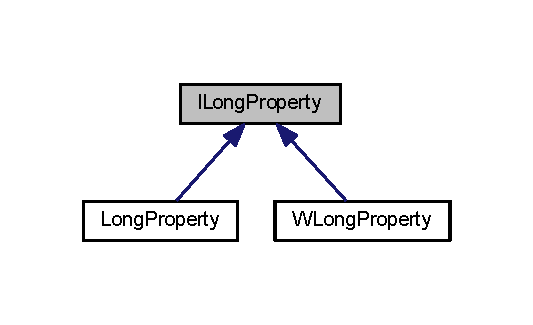
\includegraphics[width=256pt]{class_i_long_property__inherit__graph}
\end{center}
\end{figure}
\subsection*{Public Member Functions}
\begin{DoxyCompactItemize}
\item 
virtual \hyperlink{group___property_classes_ga38f1ccddda12c7cb50b868c9f789ee37}{Property\-\_\-t} \hyperlink{class_i_long_property_aff0812e50e088884a74f646f3fb3c3e7}{get\-Property\-Type} () const =0
\begin{DoxyCompactList}\small\item\em Returns the Property\-\_\-t to classify this property. \end{DoxyCompactList}\item 
virtual long \hyperlink{class_i_long_property_a52a9796a321b4453f1162fe46746bbcd}{get\-Value} (bool $\ast$success) const =0
\begin{DoxyCompactList}\small\item\em Gets this property's value as long . \end{DoxyCompactList}\item 
virtual void \hyperlink{class_i_long_property_af9aeb97712cedf69e3d517a4680ed4c2}{set\-Value} (long value)=0
\begin{DoxyCompactList}\small\item\em Sets the property's value as long . \end{DoxyCompactList}\item 
virtual bool \hyperlink{class_i_long_property_ad6eb15873636142deab4423de11e1ef8}{can\-Convert} () const =0
\begin{DoxyCompactList}\small\item\em Returns whether or not the property's value can be successfully converted. \end{DoxyCompactList}\end{DoxyCompactItemize}


\subsection{Detailed Description}
M\-A\-C\-R\-O P\-R\-O\-P\-E\-R\-T\-Y I\-N\-T\-E\-R\-F\-A\-C\-E F\-O\-R long . 

Interface for property that handles data of type long . 

\subsection{Member Function Documentation}
\hypertarget{class_i_long_property_ad6eb15873636142deab4423de11e1ef8}{\index{I\-Long\-Property@{I\-Long\-Property}!can\-Convert@{can\-Convert}}
\index{can\-Convert@{can\-Convert}!ILongProperty@{I\-Long\-Property}}
\subsubsection[{can\-Convert}]{\setlength{\rightskip}{0pt plus 5cm}virtual bool I\-Long\-Property\-::can\-Convert (
\begin{DoxyParamCaption}
{}
\end{DoxyParamCaption}
) const\hspace{0.3cm}{\ttfamily [pure virtual]}}}\label{class_i_long_property_ad6eb15873636142deab4423de11e1ef8}


Returns whether or not the property's value can be successfully converted. 

\begin{DoxyReturn}{Returns}
True if conversion is possible, false otherwise. 
\end{DoxyReturn}


Implemented in \hyperlink{class_long_property_a0ae32c7376a8a19ac6ac3010c7143f75}{Long\-Property}, and \hyperlink{class_w_long_property_af0761e534c58bf6b41776dc1298daf8a}{W\-Long\-Property}.

\hypertarget{class_i_long_property_aff0812e50e088884a74f646f3fb3c3e7}{\index{I\-Long\-Property@{I\-Long\-Property}!get\-Property\-Type@{get\-Property\-Type}}
\index{get\-Property\-Type@{get\-Property\-Type}!ILongProperty@{I\-Long\-Property}}
\subsubsection[{get\-Property\-Type}]{\setlength{\rightskip}{0pt plus 5cm}virtual {\bf Property\-\_\-t} I\-Long\-Property\-::get\-Property\-Type (
\begin{DoxyParamCaption}
{}
\end{DoxyParamCaption}
) const\hspace{0.3cm}{\ttfamily [pure virtual]}}}\label{class_i_long_property_aff0812e50e088884a74f646f3fb3c3e7}


Returns the Property\-\_\-t to classify this property. 

\begin{DoxyReturn}{Returns}
Property\-\_\-t classifier. 
\end{DoxyReturn}


Implemented in \hyperlink{class_long_property_a896acbfd359960cf26185c278b6ed85a}{Long\-Property}, and \hyperlink{class_w_long_property_a0511fc3ecd73ac409337251d7f54b1d2}{W\-Long\-Property}.

\hypertarget{class_i_long_property_a52a9796a321b4453f1162fe46746bbcd}{\index{I\-Long\-Property@{I\-Long\-Property}!get\-Value@{get\-Value}}
\index{get\-Value@{get\-Value}!ILongProperty@{I\-Long\-Property}}
\subsubsection[{get\-Value}]{\setlength{\rightskip}{0pt plus 5cm}virtual long I\-Long\-Property\-::get\-Value (
\begin{DoxyParamCaption}
\item[{bool $\ast$}]{success}
\end{DoxyParamCaption}
) const\hspace{0.3cm}{\ttfamily [pure virtual]}}}\label{class_i_long_property_a52a9796a321b4453f1162fe46746bbcd}


Gets this property's value as long . 


\begin{DoxyParams}{Parameters}
{\em success} & True if conversion was successful, false otherwise.\\
\hline
\end{DoxyParams}
\begin{DoxyReturn}{Returns}
The property's value. 
\end{DoxyReturn}


Implemented in \hyperlink{class_long_property_a6340f40f5db6887ecef15842faddbc58}{Long\-Property}, and \hyperlink{class_w_long_property_a2832bb647a51aa6688d4323e44254314}{W\-Long\-Property}.

\hypertarget{class_i_long_property_af9aeb97712cedf69e3d517a4680ed4c2}{\index{I\-Long\-Property@{I\-Long\-Property}!set\-Value@{set\-Value}}
\index{set\-Value@{set\-Value}!ILongProperty@{I\-Long\-Property}}
\subsubsection[{set\-Value}]{\setlength{\rightskip}{0pt plus 5cm}virtual void I\-Long\-Property\-::set\-Value (
\begin{DoxyParamCaption}
\item[{long}]{value}
\end{DoxyParamCaption}
)\hspace{0.3cm}{\ttfamily [pure virtual]}}}\label{class_i_long_property_af9aeb97712cedf69e3d517a4680ed4c2}


Sets the property's value as long . 


\begin{DoxyParams}{Parameters}
{\em value} & Value to set. \\
\hline
\end{DoxyParams}


Implemented in \hyperlink{class_long_property_ad39da450d5291d57af3216dfc5008c28}{Long\-Property}.



The documentation for this class was generated from the following file\-:\begin{DoxyCompactItemize}
\item 
app/\hyperlink{property_8h}{property.\-h}\end{DoxyCompactItemize}

\hypertarget{class_int_property}{\section{Int\-Property Class Reference}
\label{class_int_property}\index{Int\-Property@{Int\-Property}}
}


M\-A\-C\-R\-O P\-R\-O\-P\-E\-R\-T\-Y F\-O\-R int .  




{\ttfamily \#include $<$property.\-h$>$}



Inheritance diagram for Int\-Property\-:
\nopagebreak
\begin{figure}[H]
\begin{center}
\leavevmode
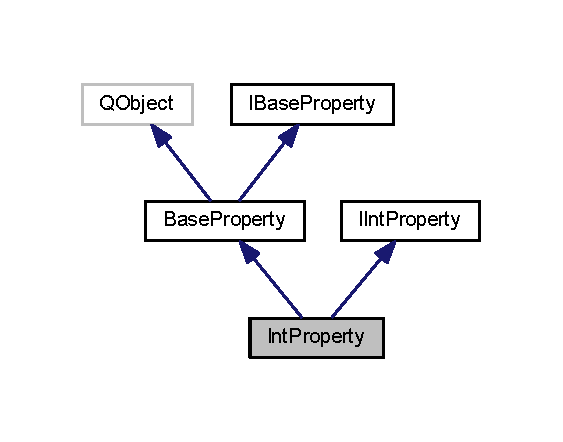
\includegraphics[width=270pt]{class_int_property__inherit__graph}
\end{center}
\end{figure}


Collaboration diagram for Int\-Property\-:
\nopagebreak
\begin{figure}[H]
\begin{center}
\leavevmode
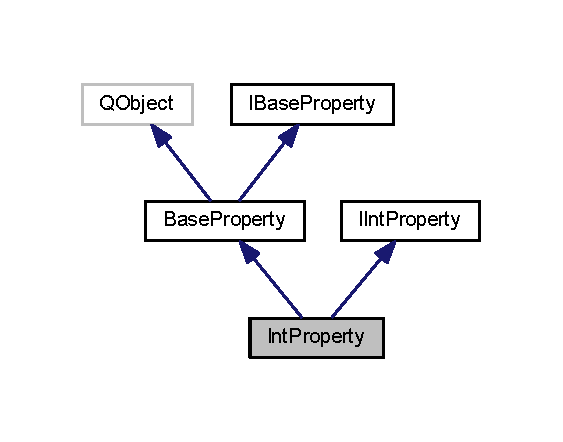
\includegraphics[width=270pt]{class_int_property__coll__graph}
\end{center}
\end{figure}
\subsection*{Public Member Functions}
\begin{DoxyCompactItemize}
\item 
\hyperlink{class_int_property_a0ac475dedc13dbe672277438328fa278}{Int\-Property} (Q\-Object $\ast$parent=0, Q\-String key=\char`\"{}\char`\"{}, int value=0, Q\-String comment=\char`\"{}\char`\"{})
\begin{DoxyCompactList}\small\item\em Constructor. Parameters not passed are initialised to safe null values. \end{DoxyCompactList}\item 
virtual \hyperlink{group___property_classes_ga38f1ccddda12c7cb50b868c9f789ee37}{Property\-\_\-t} \hyperlink{class_int_property_a3747830573f747807d40a6cb201b2137}{get\-Property\-Type} () const 
\begin{DoxyCompactList}\small\item\em Returns the Property\-\_\-t to classify this property. \end{DoxyCompactList}\item 
virtual int \hyperlink{class_int_property_a721123bb68dd46f0d0247012b663d4ba}{get\-Value} (bool $\ast$success) const 
\begin{DoxyCompactList}\small\item\em Gets this property's value as int . \end{DoxyCompactList}\item 
virtual bool \hyperlink{class_int_property_a3ce0216893c32bae0bb469fe1f82f83c}{can\-Convert} () const 
\begin{DoxyCompactList}\small\item\em Returns whether or not the property's value can be successfully converted. \end{DoxyCompactList}\item 
virtual void \hyperlink{class_int_property_a9c3b7ced3c8b7d8fbb9f739449e5622e}{set\-Value} (int value)
\begin{DoxyCompactList}\small\item\em Sets the property's value as int . \end{DoxyCompactList}\item 
virtual \hyperlink{class_w_int_property}{W\-Int\-Property} $\ast$ \hyperlink{class_int_property_a2064a016e6cb84275819e4390c7e9a84}{slots\-For} () const 
\begin{DoxyCompactList}\small\item\em Returns the interface wrapper to allow binding to slots on this property. \end{DoxyCompactList}\end{DoxyCompactItemize}
\subsection*{Additional Inherited Members}


\subsection{Detailed Description}
M\-A\-C\-R\-O P\-R\-O\-P\-E\-R\-T\-Y F\-O\-R int . 

Property that handles data of type int . 

\subsection{Constructor \& Destructor Documentation}
\hypertarget{class_int_property_a0ac475dedc13dbe672277438328fa278}{\index{Int\-Property@{Int\-Property}!Int\-Property@{Int\-Property}}
\index{Int\-Property@{Int\-Property}!IntProperty@{Int\-Property}}
\subsubsection[{Int\-Property}]{\setlength{\rightskip}{0pt plus 5cm}Int\-Property\-::\-Int\-Property (
\begin{DoxyParamCaption}
\item[{Q\-Object $\ast$}]{parent = {\ttfamily 0}, }
\item[{Q\-String}]{key = {\ttfamily \char`\"{}\char`\"{}}, }
\item[{int}]{value = {\ttfamily 0}, }
\item[{Q\-String}]{comment = {\ttfamily \char`\"{}\char`\"{}}}
\end{DoxyParamCaption}
)\hspace{0.3cm}{\ttfamily [explicit]}}}\label{class_int_property_a0ac475dedc13dbe672277438328fa278}


Constructor. Parameters not passed are initialised to safe null values. 


\begin{DoxyParams}{Parameters}
{\em parent} & Parent object for this property.\\
\hline
{\em key} & Property key (should be unique).\\
\hline
{\em value} & Property value of type int .\\
\hline
{\em comment} & Optional string comment for when this property is written into a config file. \\
\hline
\end{DoxyParams}


\subsection{Member Function Documentation}
\hypertarget{class_int_property_a3ce0216893c32bae0bb469fe1f82f83c}{\index{Int\-Property@{Int\-Property}!can\-Convert@{can\-Convert}}
\index{can\-Convert@{can\-Convert}!IntProperty@{Int\-Property}}
\subsubsection[{can\-Convert}]{\setlength{\rightskip}{0pt plus 5cm}bool Int\-Property\-::can\-Convert (
\begin{DoxyParamCaption}
{}
\end{DoxyParamCaption}
) const\hspace{0.3cm}{\ttfamily [virtual]}}}\label{class_int_property_a3ce0216893c32bae0bb469fe1f82f83c}


Returns whether or not the property's value can be successfully converted. 

\begin{DoxyReturn}{Returns}
True if conversion is possible, false otherwise. 
\end{DoxyReturn}


Implements \hyperlink{class_i_int_property_a25375f7c817ab7a1aeaef72a5bcfafdd}{I\-Int\-Property}.

\hypertarget{class_int_property_a3747830573f747807d40a6cb201b2137}{\index{Int\-Property@{Int\-Property}!get\-Property\-Type@{get\-Property\-Type}}
\index{get\-Property\-Type@{get\-Property\-Type}!IntProperty@{Int\-Property}}
\subsubsection[{get\-Property\-Type}]{\setlength{\rightskip}{0pt plus 5cm}virtual {\bf Property\-\_\-t} Int\-Property\-::get\-Property\-Type (
\begin{DoxyParamCaption}
{}
\end{DoxyParamCaption}
) const\hspace{0.3cm}{\ttfamily [inline]}, {\ttfamily [virtual]}}}\label{class_int_property_a3747830573f747807d40a6cb201b2137}


Returns the Property\-\_\-t to classify this property. 

\begin{DoxyReturn}{Returns}
Property\-\_\-t classifier. 
\end{DoxyReturn}


Implements \hyperlink{class_i_int_property_a09151bc49652e07a8b616d192d2f0401}{I\-Int\-Property}.

\hypertarget{class_int_property_a721123bb68dd46f0d0247012b663d4ba}{\index{Int\-Property@{Int\-Property}!get\-Value@{get\-Value}}
\index{get\-Value@{get\-Value}!IntProperty@{Int\-Property}}
\subsubsection[{get\-Value}]{\setlength{\rightskip}{0pt plus 5cm}int Int\-Property\-::get\-Value (
\begin{DoxyParamCaption}
\item[{bool $\ast$}]{success}
\end{DoxyParamCaption}
) const\hspace{0.3cm}{\ttfamily [virtual]}}}\label{class_int_property_a721123bb68dd46f0d0247012b663d4ba}


Gets this property's value as int . 


\begin{DoxyParams}{Parameters}
{\em success} & True if conversion was successful, false otherwise.\\
\hline
\end{DoxyParams}
\begin{DoxyReturn}{Returns}
The property's value. 
\end{DoxyReturn}


Implements \hyperlink{class_i_int_property_a32bd5be46bee5c4a53180498767f51d0}{I\-Int\-Property}.

\hypertarget{class_int_property_a9c3b7ced3c8b7d8fbb9f739449e5622e}{\index{Int\-Property@{Int\-Property}!set\-Value@{set\-Value}}
\index{set\-Value@{set\-Value}!IntProperty@{Int\-Property}}
\subsubsection[{set\-Value}]{\setlength{\rightskip}{0pt plus 5cm}void Int\-Property\-::set\-Value (
\begin{DoxyParamCaption}
\item[{int}]{value}
\end{DoxyParamCaption}
)\hspace{0.3cm}{\ttfamily [virtual]}}}\label{class_int_property_a9c3b7ced3c8b7d8fbb9f739449e5622e}


Sets the property's value as int . 


\begin{DoxyParams}{Parameters}
{\em value} & Value to set. \\
\hline
\end{DoxyParams}


Implements \hyperlink{class_i_int_property_a6ba40997660af79851cbeaff5180e61d}{I\-Int\-Property}.

\hypertarget{class_int_property_a2064a016e6cb84275819e4390c7e9a84}{\index{Int\-Property@{Int\-Property}!slots\-For@{slots\-For}}
\index{slots\-For@{slots\-For}!IntProperty@{Int\-Property}}
\subsubsection[{slots\-For}]{\setlength{\rightskip}{0pt plus 5cm}virtual {\bf W\-Int\-Property}$\ast$ Int\-Property\-::slots\-For (
\begin{DoxyParamCaption}
{}
\end{DoxyParamCaption}
) const\hspace{0.3cm}{\ttfamily [inline]}, {\ttfamily [virtual]}}}\label{class_int_property_a2064a016e6cb84275819e4390c7e9a84}


Returns the interface wrapper to allow binding to slots on this property. 

\begin{DoxyReturn}{Returns}
\hyperlink{class_w_int_property}{W\-Int\-Property} interface wrapper. 
\end{DoxyReturn}


The documentation for this class was generated from the following files\-:\begin{DoxyCompactItemize}
\item 
app/\hyperlink{property_8h}{property.\-h}\item 
app/property.\-cpp\end{DoxyCompactItemize}

\hypertarget{class_i_plugin}{\section{I\-Plugin Class Reference}
\label{class_i_plugin}\index{I\-Plugin@{I\-Plugin}}
}


Required core interface for a Crowbar plugin.  




{\ttfamily \#include $<$plugin.\-h$>$}

\subsection*{Public Member Functions}
\begin{DoxyCompactItemize}
\item 
virtual Q\-String \hyperlink{class_i_plugin_a8c0c4c970a8b59c8c7f66e1fec3045a3}{Get\-Unique\-Id} ()=0
\begin{DoxyCompactList}\small\item\em Returns the plugin's unique I\-D string. \end{DoxyCompactList}\item 
virtual Q\-String \hyperlink{class_i_plugin_a5f07a9a06d9abb95156ea70818c63386}{Get\-Author} ()=0
\begin{DoxyCompactList}\small\item\em Returns the plugin's author. \end{DoxyCompactList}\item 
virtual void \hyperlink{class_i_plugin_ae274cc3ddc9ccd4c7ee22a4da1cc2d94}{Get\-Version} (\hyperlink{plugin_8h_a725de6c68b62463ee6792bb48710febe}{Plugin\-Version} $\ast$version)=0
\begin{DoxyCompactList}\small\item\em Modifies the passed Plugin\-Version array to return this plugin's version. \end{DoxyCompactList}\end{DoxyCompactItemize}


\subsection{Detailed Description}
Required core interface for a Crowbar plugin. 

\subsection{Member Function Documentation}
\hypertarget{class_i_plugin_a5f07a9a06d9abb95156ea70818c63386}{\index{I\-Plugin@{I\-Plugin}!Get\-Author@{Get\-Author}}
\index{Get\-Author@{Get\-Author}!IPlugin@{I\-Plugin}}
\subsubsection[{Get\-Author}]{\setlength{\rightskip}{0pt plus 5cm}virtual Q\-String I\-Plugin\-::\-Get\-Author (
\begin{DoxyParamCaption}
{}
\end{DoxyParamCaption}
)\hspace{0.3cm}{\ttfamily [pure virtual]}}}\label{class_i_plugin_a5f07a9a06d9abb95156ea70818c63386}


Returns the plugin's author. 

\begin{DoxyReturn}{Returns}
Plugin's author. 
\end{DoxyReturn}
\hypertarget{class_i_plugin_a8c0c4c970a8b59c8c7f66e1fec3045a3}{\index{I\-Plugin@{I\-Plugin}!Get\-Unique\-Id@{Get\-Unique\-Id}}
\index{Get\-Unique\-Id@{Get\-Unique\-Id}!IPlugin@{I\-Plugin}}
\subsubsection[{Get\-Unique\-Id}]{\setlength{\rightskip}{0pt plus 5cm}virtual Q\-String I\-Plugin\-::\-Get\-Unique\-Id (
\begin{DoxyParamCaption}
{}
\end{DoxyParamCaption}
)\hspace{0.3cm}{\ttfamily [pure virtual]}}}\label{class_i_plugin_a8c0c4c970a8b59c8c7f66e1fec3045a3}


Returns the plugin's unique I\-D string. 

\begin{DoxyNote}{Note}
If a loaded plugin with an I\-D string already exists, subsequent plugins with this I\-D will fail to load. 
\end{DoxyNote}
\begin{DoxyReturn}{Returns}
I\-D string. 
\end{DoxyReturn}
\hypertarget{class_i_plugin_ae274cc3ddc9ccd4c7ee22a4da1cc2d94}{\index{I\-Plugin@{I\-Plugin}!Get\-Version@{Get\-Version}}
\index{Get\-Version@{Get\-Version}!IPlugin@{I\-Plugin}}
\subsubsection[{Get\-Version}]{\setlength{\rightskip}{0pt plus 5cm}virtual void I\-Plugin\-::\-Get\-Version (
\begin{DoxyParamCaption}
\item[{{\bf Plugin\-Version} $\ast$}]{version}
\end{DoxyParamCaption}
)\hspace{0.3cm}{\ttfamily [pure virtual]}}}\label{class_i_plugin_ae274cc3ddc9ccd4c7ee22a4da1cc2d94}


Modifies the passed Plugin\-Version array to return this plugin's version. 


\begin{DoxyParams}{Parameters}
{\em version} & Array to hold the plugin's version. \\
\hline
\end{DoxyParams}


The documentation for this class was generated from the following file\-:\begin{DoxyCompactItemize}
\item 
app/\hyperlink{plugin_8h}{plugin.\-h}\end{DoxyCompactItemize}

\hypertarget{class_i_string_property}{\section{I\-String\-Property Class Reference}
\label{class_i_string_property}\index{I\-String\-Property@{I\-String\-Property}}
}


M\-A\-C\-R\-O P\-R\-O\-P\-E\-R\-T\-Y I\-N\-T\-E\-R\-F\-A\-C\-E F\-O\-R Q\-String .  




{\ttfamily \#include $<$property.\-h$>$}



Inheritance diagram for I\-String\-Property\-:
\nopagebreak
\begin{figure}[H]
\begin{center}
\leavevmode
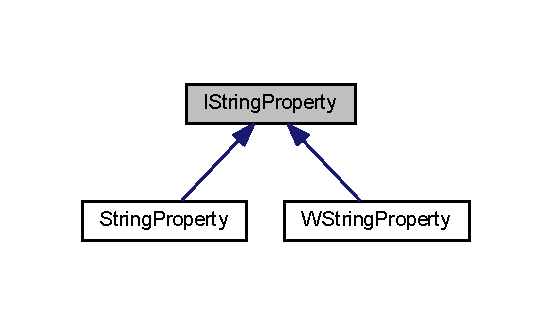
\includegraphics[width=265pt]{class_i_string_property__inherit__graph}
\end{center}
\end{figure}
\subsection*{Public Member Functions}
\begin{DoxyCompactItemize}
\item 
virtual Q\-String \hyperlink{class_i_string_property_a0dbe79993973e018510325120762504f}{get\-Value} (bool $\ast$success) const =0
\begin{DoxyCompactList}\small\item\em Gets this property's value as Q\-String . \end{DoxyCompactList}\item 
virtual void \hyperlink{class_i_string_property_a300b7403e9ce2929dabb5bb62d11142d}{set\-Value} (Q\-String value)=0
\begin{DoxyCompactList}\small\item\em Sets the property's value as Q\-String . \end{DoxyCompactList}\item 
virtual bool \hyperlink{class_i_string_property_a2fcab392710db1ae140e394c1db6739e}{can\-Convert} () const =0
\begin{DoxyCompactList}\small\item\em Returns whether or not the property's value can be successfully converted. \end{DoxyCompactList}\item 
virtual bool \hyperlink{class_i_string_property_a52c49ca31b5250fcc7914a453443b4e7}{pass\-To} (\hyperlink{class_property_variant}{Property\-Variant} $\ast$variant)=0
\begin{DoxyCompactList}\small\item\em Passes the property's value to the variant. \end{DoxyCompactList}\end{DoxyCompactItemize}


\subsection{Detailed Description}
M\-A\-C\-R\-O P\-R\-O\-P\-E\-R\-T\-Y I\-N\-T\-E\-R\-F\-A\-C\-E F\-O\-R Q\-String . 

Interface for property that handles data of type Q\-String . 

\subsection{Member Function Documentation}
\hypertarget{class_i_string_property_a2fcab392710db1ae140e394c1db6739e}{\index{I\-String\-Property@{I\-String\-Property}!can\-Convert@{can\-Convert}}
\index{can\-Convert@{can\-Convert}!IStringProperty@{I\-String\-Property}}
\subsubsection[{can\-Convert}]{\setlength{\rightskip}{0pt plus 5cm}virtual bool I\-String\-Property\-::can\-Convert (
\begin{DoxyParamCaption}
{}
\end{DoxyParamCaption}
) const\hspace{0.3cm}{\ttfamily [pure virtual]}}}\label{class_i_string_property_a2fcab392710db1ae140e394c1db6739e}


Returns whether or not the property's value can be successfully converted. 

\begin{DoxyReturn}{Returns}
True if conversion is possible, false otherwise. 
\end{DoxyReturn}


Implemented in \hyperlink{class_string_property_aa080538ba6c8ed9cfde97781dfc416cc}{String\-Property}, and \hyperlink{class_w_string_property_a6b52241cfefcea196a347bc90f57dc25}{W\-String\-Property}.

\hypertarget{class_i_string_property_a0dbe79993973e018510325120762504f}{\index{I\-String\-Property@{I\-String\-Property}!get\-Value@{get\-Value}}
\index{get\-Value@{get\-Value}!IStringProperty@{I\-String\-Property}}
\subsubsection[{get\-Value}]{\setlength{\rightskip}{0pt plus 5cm}virtual Q\-String I\-String\-Property\-::get\-Value (
\begin{DoxyParamCaption}
\item[{bool $\ast$}]{success}
\end{DoxyParamCaption}
) const\hspace{0.3cm}{\ttfamily [pure virtual]}}}\label{class_i_string_property_a0dbe79993973e018510325120762504f}


Gets this property's value as Q\-String . 


\begin{DoxyParams}{Parameters}
{\em success} & True if conversion was successful, false otherwise.\\
\hline
\end{DoxyParams}
\begin{DoxyReturn}{Returns}
The property's value. 
\end{DoxyReturn}


Implemented in \hyperlink{class_string_property_a7130232ef2d861bf098e25f47deb12cb}{String\-Property}, and \hyperlink{class_w_string_property_a4f31475a4b8cd8f7958bbfdaba6cca42}{W\-String\-Property}.

\hypertarget{class_i_string_property_a52c49ca31b5250fcc7914a453443b4e7}{\index{I\-String\-Property@{I\-String\-Property}!pass\-To@{pass\-To}}
\index{pass\-To@{pass\-To}!IStringProperty@{I\-String\-Property}}
\subsubsection[{pass\-To}]{\setlength{\rightskip}{0pt plus 5cm}virtual bool I\-String\-Property\-::pass\-To (
\begin{DoxyParamCaption}
\item[{{\bf Property\-Variant} $\ast$}]{variant}
\end{DoxyParamCaption}
)\hspace{0.3cm}{\ttfamily [pure virtual]}}}\label{class_i_string_property_a52c49ca31b5250fcc7914a453443b4e7}


Passes the property's value to the variant. 


\begin{DoxyParams}{Parameters}
{\em variant} & Variant to pass to.\\
\hline
\end{DoxyParams}
\begin{DoxyReturn}{Returns}
True if conversion succeeded, false otherwise. 
\end{DoxyReturn}
\hypertarget{class_i_string_property_a300b7403e9ce2929dabb5bb62d11142d}{\index{I\-String\-Property@{I\-String\-Property}!set\-Value@{set\-Value}}
\index{set\-Value@{set\-Value}!IStringProperty@{I\-String\-Property}}
\subsubsection[{set\-Value}]{\setlength{\rightskip}{0pt plus 5cm}virtual void I\-String\-Property\-::set\-Value (
\begin{DoxyParamCaption}
\item[{Q\-String}]{value}
\end{DoxyParamCaption}
)\hspace{0.3cm}{\ttfamily [pure virtual]}}}\label{class_i_string_property_a300b7403e9ce2929dabb5bb62d11142d}


Sets the property's value as Q\-String . 


\begin{DoxyParams}{Parameters}
{\em value} & Value to set. \\
\hline
\end{DoxyParams}


Implemented in \hyperlink{class_string_property_afebd41088d80724b87b2a1dcf41423ca}{String\-Property}.



The documentation for this class was generated from the following file\-:\begin{DoxyCompactItemize}
\item 
app/\hyperlink{property_8h}{property.\-h}\end{DoxyCompactItemize}

\hypertarget{class_i_u_int_property}{\section{I\-U\-Int\-Property Class Reference}
\label{class_i_u_int_property}\index{I\-U\-Int\-Property@{I\-U\-Int\-Property}}
}


M\-A\-C\-R\-O P\-R\-O\-P\-E\-R\-T\-Y I\-N\-T\-E\-R\-F\-A\-C\-E F\-O\-R uint .  




{\ttfamily \#include $<$property.\-h$>$}



Inheritance diagram for I\-U\-Int\-Property\-:
\nopagebreak
\begin{figure}[H]
\begin{center}
\leavevmode
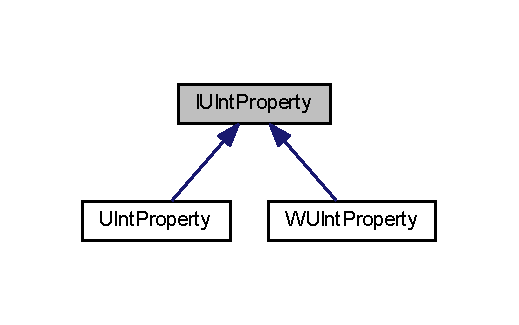
\includegraphics[width=249pt]{class_i_u_int_property__inherit__graph}
\end{center}
\end{figure}
\subsection*{Public Member Functions}
\begin{DoxyCompactItemize}
\item 
virtual uint \hyperlink{class_i_u_int_property_af3c17d292a74241f1d80b10be434edde}{get\-Value} (bool $\ast$success) const =0
\begin{DoxyCompactList}\small\item\em Gets this property's value as uint . \end{DoxyCompactList}\item 
virtual void \hyperlink{class_i_u_int_property_a2344d640892a4c3529bcca63c4c2531c}{set\-Value} (uint value)=0
\begin{DoxyCompactList}\small\item\em Sets the property's value as uint . \end{DoxyCompactList}\item 
virtual bool \hyperlink{class_i_u_int_property_a4fa6fa9ef5663109772bf51123323c87}{can\-Convert} () const =0
\begin{DoxyCompactList}\small\item\em Returns whether or not the property's value can be successfully converted. \end{DoxyCompactList}\item 
virtual bool \hyperlink{class_i_u_int_property_a1f1d04eae6cfa51bdd17157aa5dc348c}{pass\-To} (\hyperlink{class_property_variant}{Property\-Variant} $\ast$variant)=0
\begin{DoxyCompactList}\small\item\em Passes the property's value to the variant. \end{DoxyCompactList}\end{DoxyCompactItemize}


\subsection{Detailed Description}
M\-A\-C\-R\-O P\-R\-O\-P\-E\-R\-T\-Y I\-N\-T\-E\-R\-F\-A\-C\-E F\-O\-R uint . 

Interface for property that handles data of type uint . 

\subsection{Member Function Documentation}
\hypertarget{class_i_u_int_property_a4fa6fa9ef5663109772bf51123323c87}{\index{I\-U\-Int\-Property@{I\-U\-Int\-Property}!can\-Convert@{can\-Convert}}
\index{can\-Convert@{can\-Convert}!IUIntProperty@{I\-U\-Int\-Property}}
\subsubsection[{can\-Convert}]{\setlength{\rightskip}{0pt plus 5cm}virtual bool I\-U\-Int\-Property\-::can\-Convert (
\begin{DoxyParamCaption}
{}
\end{DoxyParamCaption}
) const\hspace{0.3cm}{\ttfamily [pure virtual]}}}\label{class_i_u_int_property_a4fa6fa9ef5663109772bf51123323c87}


Returns whether or not the property's value can be successfully converted. 

\begin{DoxyReturn}{Returns}
True if conversion is possible, false otherwise. 
\end{DoxyReturn}


Implemented in \hyperlink{class_u_int_property_a3f9986864fcd8cbfefd69245dc7aadfe}{U\-Int\-Property}, and \hyperlink{class_w_u_int_property_a27a4e53bf0702e796c6eecfbe9803221}{W\-U\-Int\-Property}.

\hypertarget{class_i_u_int_property_af3c17d292a74241f1d80b10be434edde}{\index{I\-U\-Int\-Property@{I\-U\-Int\-Property}!get\-Value@{get\-Value}}
\index{get\-Value@{get\-Value}!IUIntProperty@{I\-U\-Int\-Property}}
\subsubsection[{get\-Value}]{\setlength{\rightskip}{0pt plus 5cm}virtual uint I\-U\-Int\-Property\-::get\-Value (
\begin{DoxyParamCaption}
\item[{bool $\ast$}]{success}
\end{DoxyParamCaption}
) const\hspace{0.3cm}{\ttfamily [pure virtual]}}}\label{class_i_u_int_property_af3c17d292a74241f1d80b10be434edde}


Gets this property's value as uint . 


\begin{DoxyParams}{Parameters}
{\em success} & True if conversion was successful, false otherwise.\\
\hline
\end{DoxyParams}
\begin{DoxyReturn}{Returns}
The property's value. 
\end{DoxyReturn}


Implemented in \hyperlink{class_u_int_property_a9f1ce8733358de31a642990168f3f61d}{U\-Int\-Property}, and \hyperlink{class_w_u_int_property_af79534aa085135c8c642a1e929119147}{W\-U\-Int\-Property}.

\hypertarget{class_i_u_int_property_a1f1d04eae6cfa51bdd17157aa5dc348c}{\index{I\-U\-Int\-Property@{I\-U\-Int\-Property}!pass\-To@{pass\-To}}
\index{pass\-To@{pass\-To}!IUIntProperty@{I\-U\-Int\-Property}}
\subsubsection[{pass\-To}]{\setlength{\rightskip}{0pt plus 5cm}virtual bool I\-U\-Int\-Property\-::pass\-To (
\begin{DoxyParamCaption}
\item[{{\bf Property\-Variant} $\ast$}]{variant}
\end{DoxyParamCaption}
)\hspace{0.3cm}{\ttfamily [pure virtual]}}}\label{class_i_u_int_property_a1f1d04eae6cfa51bdd17157aa5dc348c}


Passes the property's value to the variant. 


\begin{DoxyParams}{Parameters}
{\em variant} & Variant to pass to.\\
\hline
\end{DoxyParams}
\begin{DoxyReturn}{Returns}
True if conversion succeeded, false otherwise. 
\end{DoxyReturn}


Implemented in \hyperlink{class_u_int_property_a05bc135083b0c2aa2ced87c2bff1ec19}{U\-Int\-Property}.

\hypertarget{class_i_u_int_property_a2344d640892a4c3529bcca63c4c2531c}{\index{I\-U\-Int\-Property@{I\-U\-Int\-Property}!set\-Value@{set\-Value}}
\index{set\-Value@{set\-Value}!IUIntProperty@{I\-U\-Int\-Property}}
\subsubsection[{set\-Value}]{\setlength{\rightskip}{0pt plus 5cm}virtual void I\-U\-Int\-Property\-::set\-Value (
\begin{DoxyParamCaption}
\item[{uint}]{value}
\end{DoxyParamCaption}
)\hspace{0.3cm}{\ttfamily [pure virtual]}}}\label{class_i_u_int_property_a2344d640892a4c3529bcca63c4c2531c}


Sets the property's value as uint . 


\begin{DoxyParams}{Parameters}
{\em value} & Value to set. \\
\hline
\end{DoxyParams}


Implemented in \hyperlink{class_u_int_property_a074ce84b6839d2451a3abee9da289198}{U\-Int\-Property}.



The documentation for this class was generated from the following file\-:\begin{DoxyCompactItemize}
\item 
app/\hyperlink{property_8h}{property.\-h}\end{DoxyCompactItemize}

\hypertarget{class_i_u_long_long_property}{\section{I\-U\-Long\-Long\-Property Class Reference}
\label{class_i_u_long_long_property}\index{I\-U\-Long\-Long\-Property@{I\-U\-Long\-Long\-Property}}
}


M\-A\-C\-R\-O P\-R\-O\-P\-E\-R\-T\-Y I\-N\-T\-E\-R\-F\-A\-C\-E F\-O\-R qulonglong .  




{\ttfamily \#include $<$property.\-h$>$}



Inheritance diagram for I\-U\-Long\-Long\-Property\-:
\nopagebreak
\begin{figure}[H]
\begin{center}
\leavevmode
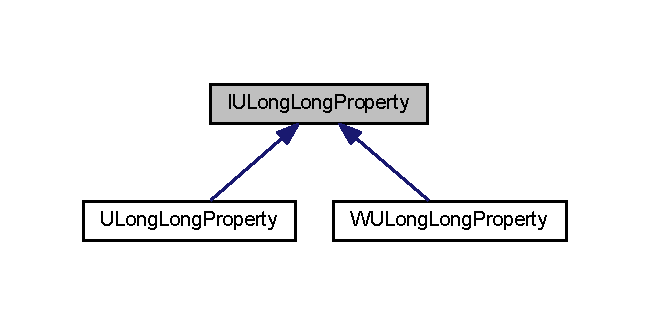
\includegraphics[width=312pt]{class_i_u_long_long_property__inherit__graph}
\end{center}
\end{figure}
\subsection*{Public Member Functions}
\begin{DoxyCompactItemize}
\item 
virtual qulonglong \hyperlink{class_i_u_long_long_property_acddc945a90cac8fa5921a9be25aaed13}{get\-Value} (bool $\ast$success) const =0
\begin{DoxyCompactList}\small\item\em Gets this property's value as qulonglong . \end{DoxyCompactList}\item 
virtual void \hyperlink{class_i_u_long_long_property_a59001a53d5cfdc3933038398fbeca269}{set\-Value} (qulonglong value)=0
\begin{DoxyCompactList}\small\item\em Sets the property's value as qulonglong . \end{DoxyCompactList}\item 
virtual bool \hyperlink{class_i_u_long_long_property_a905e766d258ebf63ed683a32aa2427a0}{can\-Convert} () const =0
\begin{DoxyCompactList}\small\item\em Returns whether or not the property's value can be successfully converted. \end{DoxyCompactList}\item 
virtual bool \hyperlink{class_i_u_long_long_property_afa78a1d7b4839a6af9c8e84fe61fb969}{pass\-To} (\hyperlink{class_property_variant}{Property\-Variant} $\ast$variant)=0
\begin{DoxyCompactList}\small\item\em Passes the property's value to the variant. \end{DoxyCompactList}\end{DoxyCompactItemize}


\subsection{Detailed Description}
M\-A\-C\-R\-O P\-R\-O\-P\-E\-R\-T\-Y I\-N\-T\-E\-R\-F\-A\-C\-E F\-O\-R qulonglong . 

Interface for property that handles data of type qulonglong . 

\subsection{Member Function Documentation}
\hypertarget{class_i_u_long_long_property_a905e766d258ebf63ed683a32aa2427a0}{\index{I\-U\-Long\-Long\-Property@{I\-U\-Long\-Long\-Property}!can\-Convert@{can\-Convert}}
\index{can\-Convert@{can\-Convert}!IULongLongProperty@{I\-U\-Long\-Long\-Property}}
\subsubsection[{can\-Convert}]{\setlength{\rightskip}{0pt plus 5cm}virtual bool I\-U\-Long\-Long\-Property\-::can\-Convert (
\begin{DoxyParamCaption}
{}
\end{DoxyParamCaption}
) const\hspace{0.3cm}{\ttfamily [pure virtual]}}}\label{class_i_u_long_long_property_a905e766d258ebf63ed683a32aa2427a0}


Returns whether or not the property's value can be successfully converted. 

\begin{DoxyReturn}{Returns}
True if conversion is possible, false otherwise. 
\end{DoxyReturn}


Implemented in \hyperlink{class_u_long_long_property_a9b670e3778650e496146c24ac133c136}{U\-Long\-Long\-Property}, and \hyperlink{class_w_u_long_long_property_a35c48d980e5e28944a9521e80e89e592}{W\-U\-Long\-Long\-Property}.

\hypertarget{class_i_u_long_long_property_acddc945a90cac8fa5921a9be25aaed13}{\index{I\-U\-Long\-Long\-Property@{I\-U\-Long\-Long\-Property}!get\-Value@{get\-Value}}
\index{get\-Value@{get\-Value}!IULongLongProperty@{I\-U\-Long\-Long\-Property}}
\subsubsection[{get\-Value}]{\setlength{\rightskip}{0pt plus 5cm}virtual qulonglong I\-U\-Long\-Long\-Property\-::get\-Value (
\begin{DoxyParamCaption}
\item[{bool $\ast$}]{success}
\end{DoxyParamCaption}
) const\hspace{0.3cm}{\ttfamily [pure virtual]}}}\label{class_i_u_long_long_property_acddc945a90cac8fa5921a9be25aaed13}


Gets this property's value as qulonglong . 


\begin{DoxyParams}{Parameters}
{\em success} & True if conversion was successful, false otherwise.\\
\hline
\end{DoxyParams}
\begin{DoxyReturn}{Returns}
The property's value. 
\end{DoxyReturn}


Implemented in \hyperlink{class_u_long_long_property_ac2dadcd92de6e92c58620ebfd1e50b66}{U\-Long\-Long\-Property}, and \hyperlink{class_w_u_long_long_property_aca6d125f5a4cd021ba353c2afd5ca31d}{W\-U\-Long\-Long\-Property}.

\hypertarget{class_i_u_long_long_property_afa78a1d7b4839a6af9c8e84fe61fb969}{\index{I\-U\-Long\-Long\-Property@{I\-U\-Long\-Long\-Property}!pass\-To@{pass\-To}}
\index{pass\-To@{pass\-To}!IULongLongProperty@{I\-U\-Long\-Long\-Property}}
\subsubsection[{pass\-To}]{\setlength{\rightskip}{0pt plus 5cm}virtual bool I\-U\-Long\-Long\-Property\-::pass\-To (
\begin{DoxyParamCaption}
\item[{{\bf Property\-Variant} $\ast$}]{variant}
\end{DoxyParamCaption}
)\hspace{0.3cm}{\ttfamily [pure virtual]}}}\label{class_i_u_long_long_property_afa78a1d7b4839a6af9c8e84fe61fb969}


Passes the property's value to the variant. 


\begin{DoxyParams}{Parameters}
{\em variant} & Variant to pass to.\\
\hline
\end{DoxyParams}
\begin{DoxyReturn}{Returns}
True if conversion succeeded, false otherwise. 
\end{DoxyReturn}


Implemented in \hyperlink{class_u_long_long_property_a501c2e699537199ef93ba3c765d3c310}{U\-Long\-Long\-Property}.

\hypertarget{class_i_u_long_long_property_a59001a53d5cfdc3933038398fbeca269}{\index{I\-U\-Long\-Long\-Property@{I\-U\-Long\-Long\-Property}!set\-Value@{set\-Value}}
\index{set\-Value@{set\-Value}!IULongLongProperty@{I\-U\-Long\-Long\-Property}}
\subsubsection[{set\-Value}]{\setlength{\rightskip}{0pt plus 5cm}virtual void I\-U\-Long\-Long\-Property\-::set\-Value (
\begin{DoxyParamCaption}
\item[{qulonglong}]{value}
\end{DoxyParamCaption}
)\hspace{0.3cm}{\ttfamily [pure virtual]}}}\label{class_i_u_long_long_property_a59001a53d5cfdc3933038398fbeca269}


Sets the property's value as qulonglong . 


\begin{DoxyParams}{Parameters}
{\em value} & Value to set. \\
\hline
\end{DoxyParams}


Implemented in \hyperlink{class_u_long_long_property_abb1dcbdd5327e7cd261df653dadcc2c9}{U\-Long\-Long\-Property}.



The documentation for this class was generated from the following file\-:\begin{DoxyCompactItemize}
\item 
app/\hyperlink{property_8h}{property.\-h}\end{DoxyCompactItemize}

\hypertarget{class_i_u_long_property}{\section{I\-U\-Long\-Property Class Reference}
\label{class_i_u_long_property}\index{I\-U\-Long\-Property@{I\-U\-Long\-Property}}
}


M\-A\-C\-R\-O P\-R\-O\-P\-E\-R\-T\-Y I\-N\-T\-E\-R\-F\-A\-C\-E F\-O\-R ulong .  




{\ttfamily \#include $<$property.\-h$>$}



Inheritance diagram for I\-U\-Long\-Property\-:
\nopagebreak
\begin{figure}[H]
\begin{center}
\leavevmode
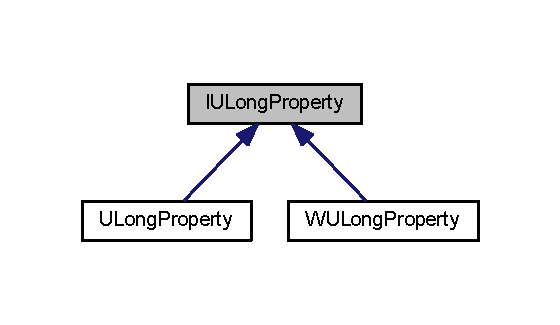
\includegraphics[width=269pt]{class_i_u_long_property__inherit__graph}
\end{center}
\end{figure}
\subsection*{Public Member Functions}
\begin{DoxyCompactItemize}
\item 
virtual \hyperlink{group___property_classes_ga38f1ccddda12c7cb50b868c9f789ee37}{Property\-\_\-t} \hyperlink{class_i_u_long_property_afcabc7c115954f9619eb2d519de1c83e}{get\-Property\-Type} () const =0
\begin{DoxyCompactList}\small\item\em Returns the Property\-\_\-t to classify this property. \end{DoxyCompactList}\item 
virtual ulong \hyperlink{class_i_u_long_property_a620e0d9b7260d93ee9e5a55c5c648f92}{get\-Value} (bool $\ast$success) const =0
\begin{DoxyCompactList}\small\item\em Gets this property's value as ulong . \end{DoxyCompactList}\item 
virtual void \hyperlink{class_i_u_long_property_a1a2b16105cd6cebdd7284ad6a631bfc4}{set\-Value} (ulong value)=0
\begin{DoxyCompactList}\small\item\em Sets the property's value as ulong . \end{DoxyCompactList}\item 
virtual bool \hyperlink{class_i_u_long_property_ad63c658df7494298fd8a0ab41623a184}{can\-Convert} () const =0
\begin{DoxyCompactList}\small\item\em Returns whether or not the property's value can be successfully converted. \end{DoxyCompactList}\end{DoxyCompactItemize}


\subsection{Detailed Description}
M\-A\-C\-R\-O P\-R\-O\-P\-E\-R\-T\-Y I\-N\-T\-E\-R\-F\-A\-C\-E F\-O\-R ulong . 

Interface for property that handles data of type ulong . 

\subsection{Member Function Documentation}
\hypertarget{class_i_u_long_property_ad63c658df7494298fd8a0ab41623a184}{\index{I\-U\-Long\-Property@{I\-U\-Long\-Property}!can\-Convert@{can\-Convert}}
\index{can\-Convert@{can\-Convert}!IULongProperty@{I\-U\-Long\-Property}}
\subsubsection[{can\-Convert}]{\setlength{\rightskip}{0pt plus 5cm}virtual bool I\-U\-Long\-Property\-::can\-Convert (
\begin{DoxyParamCaption}
{}
\end{DoxyParamCaption}
) const\hspace{0.3cm}{\ttfamily [pure virtual]}}}\label{class_i_u_long_property_ad63c658df7494298fd8a0ab41623a184}


Returns whether or not the property's value can be successfully converted. 

\begin{DoxyReturn}{Returns}
True if conversion is possible, false otherwise. 
\end{DoxyReturn}


Implemented in \hyperlink{class_u_long_property_a1ceb817d2b4fad531e3a893ad1b33273}{U\-Long\-Property}, and \hyperlink{class_w_u_long_property_add1989192edb81ac284a6680cf9f32dd}{W\-U\-Long\-Property}.

\hypertarget{class_i_u_long_property_afcabc7c115954f9619eb2d519de1c83e}{\index{I\-U\-Long\-Property@{I\-U\-Long\-Property}!get\-Property\-Type@{get\-Property\-Type}}
\index{get\-Property\-Type@{get\-Property\-Type}!IULongProperty@{I\-U\-Long\-Property}}
\subsubsection[{get\-Property\-Type}]{\setlength{\rightskip}{0pt plus 5cm}virtual {\bf Property\-\_\-t} I\-U\-Long\-Property\-::get\-Property\-Type (
\begin{DoxyParamCaption}
{}
\end{DoxyParamCaption}
) const\hspace{0.3cm}{\ttfamily [pure virtual]}}}\label{class_i_u_long_property_afcabc7c115954f9619eb2d519de1c83e}


Returns the Property\-\_\-t to classify this property. 

\begin{DoxyReturn}{Returns}
Property\-\_\-t classifier. 
\end{DoxyReturn}


Implemented in \hyperlink{class_u_long_property_aab8927e988f483d6334ba1ccffeeda99}{U\-Long\-Property}, and \hyperlink{class_w_u_long_property_a1540e17406836973ff4ffedc7ea7d294}{W\-U\-Long\-Property}.

\hypertarget{class_i_u_long_property_a620e0d9b7260d93ee9e5a55c5c648f92}{\index{I\-U\-Long\-Property@{I\-U\-Long\-Property}!get\-Value@{get\-Value}}
\index{get\-Value@{get\-Value}!IULongProperty@{I\-U\-Long\-Property}}
\subsubsection[{get\-Value}]{\setlength{\rightskip}{0pt plus 5cm}virtual ulong I\-U\-Long\-Property\-::get\-Value (
\begin{DoxyParamCaption}
\item[{bool $\ast$}]{success}
\end{DoxyParamCaption}
) const\hspace{0.3cm}{\ttfamily [pure virtual]}}}\label{class_i_u_long_property_a620e0d9b7260d93ee9e5a55c5c648f92}


Gets this property's value as ulong . 


\begin{DoxyParams}{Parameters}
{\em success} & True if conversion was successful, false otherwise.\\
\hline
\end{DoxyParams}
\begin{DoxyReturn}{Returns}
The property's value. 
\end{DoxyReturn}


Implemented in \hyperlink{class_u_long_property_a2d0ab1518fe88b2201b98dd5adf7f0a2}{U\-Long\-Property}, and \hyperlink{class_w_u_long_property_a58823102ac77872b7700b0e4347cac28}{W\-U\-Long\-Property}.

\hypertarget{class_i_u_long_property_a1a2b16105cd6cebdd7284ad6a631bfc4}{\index{I\-U\-Long\-Property@{I\-U\-Long\-Property}!set\-Value@{set\-Value}}
\index{set\-Value@{set\-Value}!IULongProperty@{I\-U\-Long\-Property}}
\subsubsection[{set\-Value}]{\setlength{\rightskip}{0pt plus 5cm}virtual void I\-U\-Long\-Property\-::set\-Value (
\begin{DoxyParamCaption}
\item[{ulong}]{value}
\end{DoxyParamCaption}
)\hspace{0.3cm}{\ttfamily [pure virtual]}}}\label{class_i_u_long_property_a1a2b16105cd6cebdd7284ad6a631bfc4}


Sets the property's value as ulong . 


\begin{DoxyParams}{Parameters}
{\em value} & Value to set. \\
\hline
\end{DoxyParams}


Implemented in \hyperlink{class_u_long_property_ac52a81a11a65723ab008ba066be522f3}{U\-Long\-Property}.



The documentation for this class was generated from the following file\-:\begin{DoxyCompactItemize}
\item 
app/\hyperlink{property_8h}{property.\-h}\end{DoxyCompactItemize}

\hypertarget{class_log_window}{\section{Log\-Window Class Reference}
\label{class_log_window}\index{Log\-Window@{Log\-Window}}
}


Logging window.  




{\ttfamily \#include $<$logwindow.\-h$>$}



Inheritance diagram for Log\-Window\-:
\nopagebreak
\begin{figure}[H]
\begin{center}
\leavevmode
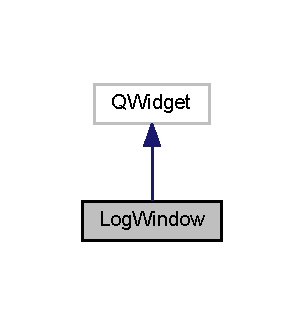
\includegraphics[width=146pt]{class_log_window__inherit__graph}
\end{center}
\end{figure}


Collaboration diagram for Log\-Window\-:
\nopagebreak
\begin{figure}[H]
\begin{center}
\leavevmode
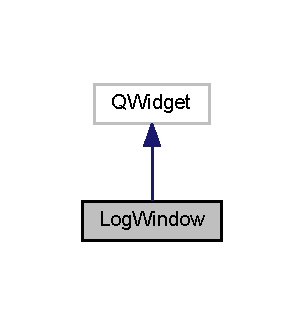
\includegraphics[width=146pt]{class_log_window__coll__graph}
\end{center}
\end{figure}
\subsection*{Public Slots}
\begin{DoxyCompactItemize}
\item 
\hypertarget{class_log_window_adcc6e0cdf92339342b6d564969c9c08a}{void \hyperlink{class_log_window_adcc6e0cdf92339342b6d564969c9c08a}{show} ()}\label{class_log_window_adcc6e0cdf92339342b6d564969c9c08a}

\begin{DoxyCompactList}\small\item\em Shows the logging window. \end{DoxyCompactList}\item 
\hypertarget{class_log_window_a0e2b0c1b3532f71fbff15d038417f108}{void \hyperlink{class_log_window_a0e2b0c1b3532f71fbff15d038417f108}{show\-And\-Raise} ()}\label{class_log_window_a0e2b0c1b3532f71fbff15d038417f108}

\begin{DoxyCompactList}\small\item\em Shows the logging window and raises it to be on top of any other windows. \end{DoxyCompactList}\item 
void \hyperlink{class_log_window_ac001882d402237088e250734cd98838c}{print\-Message} (Q\-String message)
\begin{DoxyCompactList}\small\item\em Prints a message to the log window (but not to a log file). \end{DoxyCompactList}\item 
void \hyperlink{class_log_window_ad22aacde45b6bbb323a7f2a4d8aba94b}{log\-Message} (Q\-String message)
\begin{DoxyCompactList}\small\item\em Writes a message to a log file (but does not print to the log window). \end{DoxyCompactList}\item 
void \hyperlink{class_log_window_a6e465543f32c1b9447ccbb481eee9407}{print\-Warning} (Q\-String message)
\begin{DoxyCompactList}\small\item\em Prints a warning to the log window (but not to a log file). \end{DoxyCompactList}\item 
void \hyperlink{class_log_window_adde69360b38aad4e23ee16100adba710}{log\-Warning} (Q\-String message)
\begin{DoxyCompactList}\small\item\em Writes a warning to a log file (but does not print to the log window). \end{DoxyCompactList}\item 
\hypertarget{class_log_window_af2db9c420af21e1c07b416a6a3a7e5a2}{void \hyperlink{class_log_window_af2db9c420af21e1c07b416a6a3a7e5a2}{zoom\-In} ()}\label{class_log_window_af2db9c420af21e1c07b416a6a3a7e5a2}

\begin{DoxyCompactList}\small\item\em Makes the log window text larger. \end{DoxyCompactList}\item 
\hypertarget{class_log_window_ae534c7a6486b7223427dc2ad65316b09}{void \hyperlink{class_log_window_ae534c7a6486b7223427dc2ad65316b09}{zoom\-Out} ()}\label{class_log_window_ae534c7a6486b7223427dc2ad65316b09}

\begin{DoxyCompactList}\small\item\em Makes the log window text smaller. \end{DoxyCompactList}\item 
\hypertarget{class_log_window_a18658a91b3a65b744a684994ab247dde}{void \hyperlink{class_log_window_a18658a91b3a65b744a684994ab247dde}{new\-Log\-File} ()}\label{class_log_window_a18658a91b3a65b744a684994ab247dde}

\begin{DoxyCompactList}\small\item\em Creates a new log file whose name is based on the current date and time. \end{DoxyCompactList}\item 
void \hyperlink{class_log_window_a903fc2156c1aa3f72c28fff20ecee6e3}{new\-Log\-File} (Q\-String filename)
\begin{DoxyCompactList}\small\item\em Creates a new log file. \end{DoxyCompactList}\end{DoxyCompactItemize}
\subsection*{Public Member Functions}
\begin{DoxyCompactItemize}
\item 
\hyperlink{class_log_window_a3c1a4587d8e7ee120db18abf0184ca22}{Log\-Window} (Q\-Widget $\ast$parent=0)
\begin{DoxyCompactList}\small\item\em Constructor. \end{DoxyCompactList}\item 
\hypertarget{class_log_window_a8c96adb435e3e88f42396876f6213527}{\hyperlink{class_log_window_a8c96adb435e3e88f42396876f6213527}{$\sim$\-Log\-Window} ()}\label{class_log_window_a8c96adb435e3e88f42396876f6213527}

\begin{DoxyCompactList}\small\item\em Destructor. \end{DoxyCompactList}\item 
Q\-String \hyperlink{class_log_window_a7c9598991e02625f315613690b65d33b}{Get\-Log\-File\-Name} () const 
\begin{DoxyCompactList}\small\item\em Returns the name of the current log file. \end{DoxyCompactList}\end{DoxyCompactItemize}


\subsection{Detailed Description}
Logging window. 

If the application is started in debug mode, the logging window will be shown as well as any application windows. Part of the application can send log messages which will be printed to this window and logged into a file. The log window can be re-\/opened from the Debug menu in an application window if it is closed. If logging is enabled without debug mode, any messages will be sent to a log file but the log window and the Debug menu will not be shown. 

\subsection{Constructor \& Destructor Documentation}
\hypertarget{class_log_window_a3c1a4587d8e7ee120db18abf0184ca22}{\index{Log\-Window@{Log\-Window}!Log\-Window@{Log\-Window}}
\index{Log\-Window@{Log\-Window}!LogWindow@{Log\-Window}}
\subsubsection[{Log\-Window}]{\setlength{\rightskip}{0pt plus 5cm}Log\-Window\-::\-Log\-Window (
\begin{DoxyParamCaption}
\item[{Q\-Widget $\ast$}]{parent = {\ttfamily 0}}
\end{DoxyParamCaption}
)\hspace{0.3cm}{\ttfamily [explicit]}}}\label{class_log_window_a3c1a4587d8e7ee120db18abf0184ca22}


Constructor. 


\begin{DoxyParams}{Parameters}
{\em parent} & Parent object (usually N\-U\-L\-L). \\
\hline
\end{DoxyParams}


\subsection{Member Function Documentation}
\hypertarget{class_log_window_a7c9598991e02625f315613690b65d33b}{\index{Log\-Window@{Log\-Window}!Get\-Log\-File\-Name@{Get\-Log\-File\-Name}}
\index{Get\-Log\-File\-Name@{Get\-Log\-File\-Name}!LogWindow@{Log\-Window}}
\subsubsection[{Get\-Log\-File\-Name}]{\setlength{\rightskip}{0pt plus 5cm}Q\-String Log\-Window\-::\-Get\-Log\-File\-Name (
\begin{DoxyParamCaption}
{}
\end{DoxyParamCaption}
) const}}\label{class_log_window_a7c9598991e02625f315613690b65d33b}


Returns the name of the current log file. 

\begin{DoxyReturn}{Returns}
Name of the log file, or \char`\"{}\char`\"{} if no file is currently open. 
\end{DoxyReturn}
\hypertarget{class_log_window_ad22aacde45b6bbb323a7f2a4d8aba94b}{\index{Log\-Window@{Log\-Window}!log\-Message@{log\-Message}}
\index{log\-Message@{log\-Message}!LogWindow@{Log\-Window}}
\subsubsection[{log\-Message}]{\setlength{\rightskip}{0pt plus 5cm}void Log\-Window\-::log\-Message (
\begin{DoxyParamCaption}
\item[{Q\-String}]{message}
\end{DoxyParamCaption}
)\hspace{0.3cm}{\ttfamily [slot]}}}\label{class_log_window_ad22aacde45b6bbb323a7f2a4d8aba94b}


Writes a message to a log file (but does not print to the log window). 


\begin{DoxyParams}{Parameters}
{\em message} & Message to print. \\
\hline
\end{DoxyParams}
\hypertarget{class_log_window_adde69360b38aad4e23ee16100adba710}{\index{Log\-Window@{Log\-Window}!log\-Warning@{log\-Warning}}
\index{log\-Warning@{log\-Warning}!LogWindow@{Log\-Window}}
\subsubsection[{log\-Warning}]{\setlength{\rightskip}{0pt plus 5cm}void Log\-Window\-::log\-Warning (
\begin{DoxyParamCaption}
\item[{Q\-String}]{message}
\end{DoxyParamCaption}
)\hspace{0.3cm}{\ttfamily [slot]}}}\label{class_log_window_adde69360b38aad4e23ee16100adba710}


Writes a warning to a log file (but does not print to the log window). 


\begin{DoxyParams}{Parameters}
{\em message} & Message to print. \\
\hline
\end{DoxyParams}
\hypertarget{class_log_window_a903fc2156c1aa3f72c28fff20ecee6e3}{\index{Log\-Window@{Log\-Window}!new\-Log\-File@{new\-Log\-File}}
\index{new\-Log\-File@{new\-Log\-File}!LogWindow@{Log\-Window}}
\subsubsection[{new\-Log\-File}]{\setlength{\rightskip}{0pt plus 5cm}void Log\-Window\-::new\-Log\-File (
\begin{DoxyParamCaption}
\item[{Q\-String}]{filename}
\end{DoxyParamCaption}
)\hspace{0.3cm}{\ttfamily [slot]}}}\label{class_log_window_a903fc2156c1aa3f72c28fff20ecee6e3}


Creates a new log file. 


\begin{DoxyParams}{Parameters}
{\em filename} & Name of file to create. \\
\hline
\end{DoxyParams}
\hypertarget{class_log_window_ac001882d402237088e250734cd98838c}{\index{Log\-Window@{Log\-Window}!print\-Message@{print\-Message}}
\index{print\-Message@{print\-Message}!LogWindow@{Log\-Window}}
\subsubsection[{print\-Message}]{\setlength{\rightskip}{0pt plus 5cm}void Log\-Window\-::print\-Message (
\begin{DoxyParamCaption}
\item[{Q\-String}]{message}
\end{DoxyParamCaption}
)\hspace{0.3cm}{\ttfamily [slot]}}}\label{class_log_window_ac001882d402237088e250734cd98838c}


Prints a message to the log window (but not to a log file). 


\begin{DoxyParams}{Parameters}
{\em message} & Message to print. \\
\hline
\end{DoxyParams}
\hypertarget{class_log_window_a6e465543f32c1b9447ccbb481eee9407}{\index{Log\-Window@{Log\-Window}!print\-Warning@{print\-Warning}}
\index{print\-Warning@{print\-Warning}!LogWindow@{Log\-Window}}
\subsubsection[{print\-Warning}]{\setlength{\rightskip}{0pt plus 5cm}void Log\-Window\-::print\-Warning (
\begin{DoxyParamCaption}
\item[{Q\-String}]{message}
\end{DoxyParamCaption}
)\hspace{0.3cm}{\ttfamily [slot]}}}\label{class_log_window_a6e465543f32c1b9447ccbb481eee9407}


Prints a warning to the log window (but not to a log file). 


\begin{DoxyParams}{Parameters}
{\em message} & Message to print. \\
\hline
\end{DoxyParams}


The documentation for this class was generated from the following files\-:\begin{DoxyCompactItemize}
\item 
app/\hyperlink{logwindow_8h}{logwindow.\-h}\item 
app/logwindow.\-cpp\end{DoxyCompactItemize}

\hypertarget{class_long_long_property}{\section{Long\-Long\-Property Class Reference}
\label{class_long_long_property}\index{Long\-Long\-Property@{Long\-Long\-Property}}
}


M\-A\-C\-R\-O P\-R\-O\-P\-E\-R\-T\-Y F\-O\-R qlonglong .  




{\ttfamily \#include $<$property.\-h$>$}



Inheritance diagram for Long\-Long\-Property\-:
\nopagebreak
\begin{figure}[H]
\begin{center}
\leavevmode
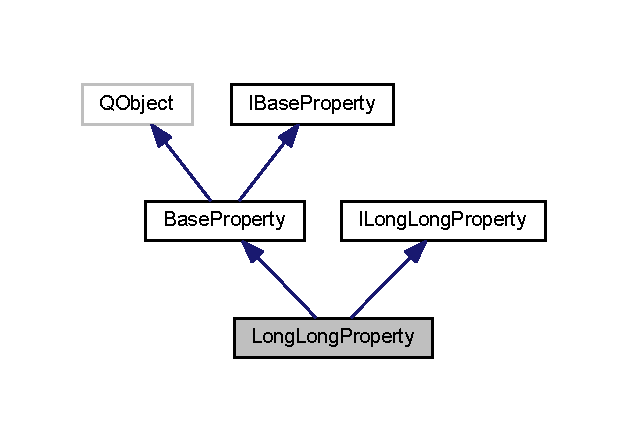
\includegraphics[width=302pt]{class_long_long_property__inherit__graph}
\end{center}
\end{figure}


Collaboration diagram for Long\-Long\-Property\-:
\nopagebreak
\begin{figure}[H]
\begin{center}
\leavevmode
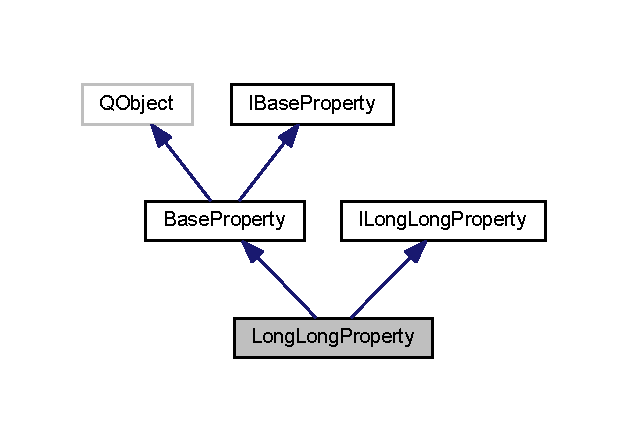
\includegraphics[width=302pt]{class_long_long_property__coll__graph}
\end{center}
\end{figure}
\subsection*{Public Member Functions}
\begin{DoxyCompactItemize}
\item 
\hyperlink{class_long_long_property_af3527fb08c50e565e669966774ad1254}{Long\-Long\-Property} (Q\-Object $\ast$parent=0, Q\-String key=\char`\"{}\char`\"{}, qlonglong value=0, Q\-String comment=\char`\"{}\char`\"{})
\begin{DoxyCompactList}\small\item\em Constructor. Parameters not passed are initialised to safe null values. \end{DoxyCompactList}\item 
virtual \hyperlink{group___property_classes_ga38f1ccddda12c7cb50b868c9f789ee37}{Property\-\_\-t} \hyperlink{class_long_long_property_aef541867fa0047705e5ceb968da5073d}{get\-Property\-Type} () const 
\begin{DoxyCompactList}\small\item\em Returns the Property\-\_\-t to classify this property. \end{DoxyCompactList}\item 
virtual qlonglong \hyperlink{class_long_long_property_a55da84c1e1c5db5431a3b5ddae6a72eb}{get\-Value} (bool $\ast$success) const 
\begin{DoxyCompactList}\small\item\em Gets this property's value as qlonglong . \end{DoxyCompactList}\item 
virtual bool \hyperlink{class_long_long_property_a2690f56d6b804d37eec1457250da4acb}{can\-Convert} () const 
\begin{DoxyCompactList}\small\item\em Returns whether or not the property's value can be successfully converted. \end{DoxyCompactList}\item 
virtual void \hyperlink{class_long_long_property_abff074961b681f08072260664b0221f6}{set\-Value} (qlonglong value)
\begin{DoxyCompactList}\small\item\em Sets the property's value as qlonglong . \end{DoxyCompactList}\item 
virtual \hyperlink{class_w_long_long_property}{W\-Long\-Long\-Property} $\ast$ \hyperlink{class_long_long_property_a1a835b6e035572c098c27b21931c3d7f}{slots\-For} () const 
\begin{DoxyCompactList}\small\item\em Returns the interface wrapper to allow binding to slots on this property. \end{DoxyCompactList}\end{DoxyCompactItemize}
\subsection*{Additional Inherited Members}


\subsection{Detailed Description}
M\-A\-C\-R\-O P\-R\-O\-P\-E\-R\-T\-Y F\-O\-R qlonglong . 

Property that handles data of type qlonglong . 

\subsection{Constructor \& Destructor Documentation}
\hypertarget{class_long_long_property_af3527fb08c50e565e669966774ad1254}{\index{Long\-Long\-Property@{Long\-Long\-Property}!Long\-Long\-Property@{Long\-Long\-Property}}
\index{Long\-Long\-Property@{Long\-Long\-Property}!LongLongProperty@{Long\-Long\-Property}}
\subsubsection[{Long\-Long\-Property}]{\setlength{\rightskip}{0pt plus 5cm}Long\-Long\-Property\-::\-Long\-Long\-Property (
\begin{DoxyParamCaption}
\item[{Q\-Object $\ast$}]{parent = {\ttfamily 0}, }
\item[{Q\-String}]{key = {\ttfamily \char`\"{}\char`\"{}}, }
\item[{qlonglong}]{value = {\ttfamily 0}, }
\item[{Q\-String}]{comment = {\ttfamily \char`\"{}\char`\"{}}}
\end{DoxyParamCaption}
)\hspace{0.3cm}{\ttfamily [explicit]}}}\label{class_long_long_property_af3527fb08c50e565e669966774ad1254}


Constructor. Parameters not passed are initialised to safe null values. 


\begin{DoxyParams}{Parameters}
{\em parent} & Parent object for this property.\\
\hline
{\em key} & Property key (should be unique).\\
\hline
{\em value} & Property value of type qlonglong .\\
\hline
{\em comment} & Optional string comment for when this property is written into a config file. \\
\hline
\end{DoxyParams}


\subsection{Member Function Documentation}
\hypertarget{class_long_long_property_a2690f56d6b804d37eec1457250da4acb}{\index{Long\-Long\-Property@{Long\-Long\-Property}!can\-Convert@{can\-Convert}}
\index{can\-Convert@{can\-Convert}!LongLongProperty@{Long\-Long\-Property}}
\subsubsection[{can\-Convert}]{\setlength{\rightskip}{0pt plus 5cm}bool Long\-Long\-Property\-::can\-Convert (
\begin{DoxyParamCaption}
{}
\end{DoxyParamCaption}
) const\hspace{0.3cm}{\ttfamily [virtual]}}}\label{class_long_long_property_a2690f56d6b804d37eec1457250da4acb}


Returns whether or not the property's value can be successfully converted. 

\begin{DoxyReturn}{Returns}
True if conversion is possible, false otherwise. 
\end{DoxyReturn}


Implements \hyperlink{class_i_long_long_property_a878b7753e3c53e966f9be8a3bd1e9b38}{I\-Long\-Long\-Property}.

\hypertarget{class_long_long_property_aef541867fa0047705e5ceb968da5073d}{\index{Long\-Long\-Property@{Long\-Long\-Property}!get\-Property\-Type@{get\-Property\-Type}}
\index{get\-Property\-Type@{get\-Property\-Type}!LongLongProperty@{Long\-Long\-Property}}
\subsubsection[{get\-Property\-Type}]{\setlength{\rightskip}{0pt plus 5cm}virtual {\bf Property\-\_\-t} Long\-Long\-Property\-::get\-Property\-Type (
\begin{DoxyParamCaption}
{}
\end{DoxyParamCaption}
) const\hspace{0.3cm}{\ttfamily [inline]}, {\ttfamily [virtual]}}}\label{class_long_long_property_aef541867fa0047705e5ceb968da5073d}


Returns the Property\-\_\-t to classify this property. 

\begin{DoxyReturn}{Returns}
Property\-\_\-t classifier. 
\end{DoxyReturn}


Implements \hyperlink{class_i_long_long_property_a799afb367a1ec4c8cf651d61abf782d6}{I\-Long\-Long\-Property}.

\hypertarget{class_long_long_property_a55da84c1e1c5db5431a3b5ddae6a72eb}{\index{Long\-Long\-Property@{Long\-Long\-Property}!get\-Value@{get\-Value}}
\index{get\-Value@{get\-Value}!LongLongProperty@{Long\-Long\-Property}}
\subsubsection[{get\-Value}]{\setlength{\rightskip}{0pt plus 5cm}qlonglong Long\-Long\-Property\-::get\-Value (
\begin{DoxyParamCaption}
\item[{bool $\ast$}]{success}
\end{DoxyParamCaption}
) const\hspace{0.3cm}{\ttfamily [virtual]}}}\label{class_long_long_property_a55da84c1e1c5db5431a3b5ddae6a72eb}


Gets this property's value as qlonglong . 


\begin{DoxyParams}{Parameters}
{\em success} & True if conversion was successful, false otherwise.\\
\hline
\end{DoxyParams}
\begin{DoxyReturn}{Returns}
The property's value. 
\end{DoxyReturn}


Implements \hyperlink{class_i_long_long_property_a4364152258a2b085fa660ae34d106fdf}{I\-Long\-Long\-Property}.

\hypertarget{class_long_long_property_abff074961b681f08072260664b0221f6}{\index{Long\-Long\-Property@{Long\-Long\-Property}!set\-Value@{set\-Value}}
\index{set\-Value@{set\-Value}!LongLongProperty@{Long\-Long\-Property}}
\subsubsection[{set\-Value}]{\setlength{\rightskip}{0pt plus 5cm}void Long\-Long\-Property\-::set\-Value (
\begin{DoxyParamCaption}
\item[{qlonglong}]{value}
\end{DoxyParamCaption}
)\hspace{0.3cm}{\ttfamily [virtual]}}}\label{class_long_long_property_abff074961b681f08072260664b0221f6}


Sets the property's value as qlonglong . 


\begin{DoxyParams}{Parameters}
{\em value} & Value to set. \\
\hline
\end{DoxyParams}


Implements \hyperlink{class_i_long_long_property_a3ef096db3b5d53b1566148d9c78fcbbf}{I\-Long\-Long\-Property}.

\hypertarget{class_long_long_property_a1a835b6e035572c098c27b21931c3d7f}{\index{Long\-Long\-Property@{Long\-Long\-Property}!slots\-For@{slots\-For}}
\index{slots\-For@{slots\-For}!LongLongProperty@{Long\-Long\-Property}}
\subsubsection[{slots\-For}]{\setlength{\rightskip}{0pt plus 5cm}virtual {\bf W\-Long\-Long\-Property}$\ast$ Long\-Long\-Property\-::slots\-For (
\begin{DoxyParamCaption}
{}
\end{DoxyParamCaption}
) const\hspace{0.3cm}{\ttfamily [inline]}, {\ttfamily [virtual]}}}\label{class_long_long_property_a1a835b6e035572c098c27b21931c3d7f}


Returns the interface wrapper to allow binding to slots on this property. 

\begin{DoxyReturn}{Returns}
\hyperlink{class_w_long_long_property}{W\-Long\-Long\-Property} interface wrapper. 
\end{DoxyReturn}


The documentation for this class was generated from the following files\-:\begin{DoxyCompactItemize}
\item 
app/\hyperlink{property_8h}{property.\-h}\item 
app/property.\-cpp\end{DoxyCompactItemize}

\hypertarget{class_long_property}{\section{Long\-Property Class Reference}
\label{class_long_property}\index{Long\-Property@{Long\-Property}}
}


M\-A\-C\-R\-O P\-R\-O\-P\-E\-R\-T\-Y F\-O\-R long .  




{\ttfamily \#include $<$property.\-h$>$}



Inheritance diagram for Long\-Property\-:
\nopagebreak
\begin{figure}[H]
\begin{center}
\leavevmode
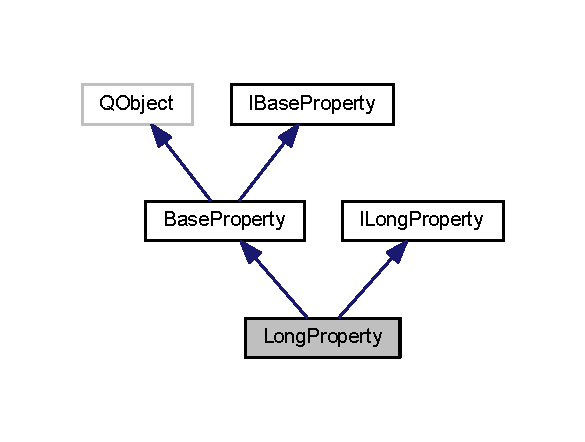
\includegraphics[width=281pt]{class_long_property__inherit__graph}
\end{center}
\end{figure}


Collaboration diagram for Long\-Property\-:
\nopagebreak
\begin{figure}[H]
\begin{center}
\leavevmode
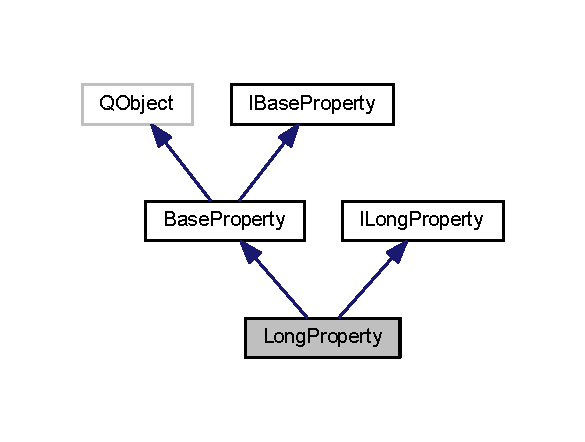
\includegraphics[width=281pt]{class_long_property__coll__graph}
\end{center}
\end{figure}
\subsection*{Public Member Functions}
\begin{DoxyCompactItemize}
\item 
\hyperlink{class_long_property_a9c4b842a60dce4d158af82e74d877492}{Long\-Property} (Q\-Object $\ast$parent=0, Q\-String key=\char`\"{}\char`\"{}, long value=0, Q\-String comment=\char`\"{}\char`\"{})
\begin{DoxyCompactList}\small\item\em Constructor. Parameters not passed are initialised to safe null values. \end{DoxyCompactList}\item 
virtual \hyperlink{group___property_classes_ga38f1ccddda12c7cb50b868c9f789ee37}{Property\-\_\-t} \hyperlink{class_long_property_a896acbfd359960cf26185c278b6ed85a}{get\-Property\-Type} () const 
\begin{DoxyCompactList}\small\item\em Returns the Property\-\_\-t to classify this property. \end{DoxyCompactList}\item 
virtual long \hyperlink{class_long_property_a6340f40f5db6887ecef15842faddbc58}{get\-Value} (bool $\ast$success) const 
\begin{DoxyCompactList}\small\item\em Gets this property's value as long . \end{DoxyCompactList}\item 
virtual bool \hyperlink{class_long_property_a0ae32c7376a8a19ac6ac3010c7143f75}{can\-Convert} () const 
\begin{DoxyCompactList}\small\item\em Returns whether or not the property's value can be successfully converted. \end{DoxyCompactList}\item 
virtual void \hyperlink{class_long_property_ad39da450d5291d57af3216dfc5008c28}{set\-Value} (long value)
\begin{DoxyCompactList}\small\item\em Sets the property's value as long . \end{DoxyCompactList}\item 
virtual \hyperlink{class_w_long_property}{W\-Long\-Property} $\ast$ \hyperlink{class_long_property_a0819c723cc3341f44390bb8e4a88d509}{slots\-For} () const 
\begin{DoxyCompactList}\small\item\em Returns the interface wrapper to allow binding to slots on this property. \end{DoxyCompactList}\end{DoxyCompactItemize}
\subsection*{Additional Inherited Members}


\subsection{Detailed Description}
M\-A\-C\-R\-O P\-R\-O\-P\-E\-R\-T\-Y F\-O\-R long . 

Property that handles data of type long . 

\subsection{Constructor \& Destructor Documentation}
\hypertarget{class_long_property_a9c4b842a60dce4d158af82e74d877492}{\index{Long\-Property@{Long\-Property}!Long\-Property@{Long\-Property}}
\index{Long\-Property@{Long\-Property}!LongProperty@{Long\-Property}}
\subsubsection[{Long\-Property}]{\setlength{\rightskip}{0pt plus 5cm}Long\-Property\-::\-Long\-Property (
\begin{DoxyParamCaption}
\item[{Q\-Object $\ast$}]{parent = {\ttfamily 0}, }
\item[{Q\-String}]{key = {\ttfamily \char`\"{}\char`\"{}}, }
\item[{long}]{value = {\ttfamily 0}, }
\item[{Q\-String}]{comment = {\ttfamily \char`\"{}\char`\"{}}}
\end{DoxyParamCaption}
)\hspace{0.3cm}{\ttfamily [explicit]}}}\label{class_long_property_a9c4b842a60dce4d158af82e74d877492}


Constructor. Parameters not passed are initialised to safe null values. 


\begin{DoxyParams}{Parameters}
{\em parent} & Parent object for this property.\\
\hline
{\em key} & Property key (should be unique).\\
\hline
{\em value} & Property value of type long .\\
\hline
{\em comment} & Optional string comment for when this property is written into a config file. \\
\hline
\end{DoxyParams}


\subsection{Member Function Documentation}
\hypertarget{class_long_property_a0ae32c7376a8a19ac6ac3010c7143f75}{\index{Long\-Property@{Long\-Property}!can\-Convert@{can\-Convert}}
\index{can\-Convert@{can\-Convert}!LongProperty@{Long\-Property}}
\subsubsection[{can\-Convert}]{\setlength{\rightskip}{0pt plus 5cm}bool Long\-Property\-::can\-Convert (
\begin{DoxyParamCaption}
{}
\end{DoxyParamCaption}
) const\hspace{0.3cm}{\ttfamily [virtual]}}}\label{class_long_property_a0ae32c7376a8a19ac6ac3010c7143f75}


Returns whether or not the property's value can be successfully converted. 

\begin{DoxyReturn}{Returns}
True if conversion is possible, false otherwise. 
\end{DoxyReturn}


Implements \hyperlink{class_i_long_property_ad6eb15873636142deab4423de11e1ef8}{I\-Long\-Property}.

\hypertarget{class_long_property_a896acbfd359960cf26185c278b6ed85a}{\index{Long\-Property@{Long\-Property}!get\-Property\-Type@{get\-Property\-Type}}
\index{get\-Property\-Type@{get\-Property\-Type}!LongProperty@{Long\-Property}}
\subsubsection[{get\-Property\-Type}]{\setlength{\rightskip}{0pt plus 5cm}virtual {\bf Property\-\_\-t} Long\-Property\-::get\-Property\-Type (
\begin{DoxyParamCaption}
{}
\end{DoxyParamCaption}
) const\hspace{0.3cm}{\ttfamily [inline]}, {\ttfamily [virtual]}}}\label{class_long_property_a896acbfd359960cf26185c278b6ed85a}


Returns the Property\-\_\-t to classify this property. 

\begin{DoxyReturn}{Returns}
Property\-\_\-t classifier. 
\end{DoxyReturn}


Implements \hyperlink{class_i_long_property_aff0812e50e088884a74f646f3fb3c3e7}{I\-Long\-Property}.

\hypertarget{class_long_property_a6340f40f5db6887ecef15842faddbc58}{\index{Long\-Property@{Long\-Property}!get\-Value@{get\-Value}}
\index{get\-Value@{get\-Value}!LongProperty@{Long\-Property}}
\subsubsection[{get\-Value}]{\setlength{\rightskip}{0pt plus 5cm}long Long\-Property\-::get\-Value (
\begin{DoxyParamCaption}
\item[{bool $\ast$}]{success}
\end{DoxyParamCaption}
) const\hspace{0.3cm}{\ttfamily [virtual]}}}\label{class_long_property_a6340f40f5db6887ecef15842faddbc58}


Gets this property's value as long . 


\begin{DoxyParams}{Parameters}
{\em success} & True if conversion was successful, false otherwise.\\
\hline
\end{DoxyParams}
\begin{DoxyReturn}{Returns}
The property's value. 
\end{DoxyReturn}


Implements \hyperlink{class_i_long_property_a52a9796a321b4453f1162fe46746bbcd}{I\-Long\-Property}.

\hypertarget{class_long_property_ad39da450d5291d57af3216dfc5008c28}{\index{Long\-Property@{Long\-Property}!set\-Value@{set\-Value}}
\index{set\-Value@{set\-Value}!LongProperty@{Long\-Property}}
\subsubsection[{set\-Value}]{\setlength{\rightskip}{0pt plus 5cm}void Long\-Property\-::set\-Value (
\begin{DoxyParamCaption}
\item[{long}]{value}
\end{DoxyParamCaption}
)\hspace{0.3cm}{\ttfamily [virtual]}}}\label{class_long_property_ad39da450d5291d57af3216dfc5008c28}


Sets the property's value as long . 


\begin{DoxyParams}{Parameters}
{\em value} & Value to set. \\
\hline
\end{DoxyParams}


Implements \hyperlink{class_i_long_property_af9aeb97712cedf69e3d517a4680ed4c2}{I\-Long\-Property}.

\hypertarget{class_long_property_a0819c723cc3341f44390bb8e4a88d509}{\index{Long\-Property@{Long\-Property}!slots\-For@{slots\-For}}
\index{slots\-For@{slots\-For}!LongProperty@{Long\-Property}}
\subsubsection[{slots\-For}]{\setlength{\rightskip}{0pt plus 5cm}virtual {\bf W\-Long\-Property}$\ast$ Long\-Property\-::slots\-For (
\begin{DoxyParamCaption}
{}
\end{DoxyParamCaption}
) const\hspace{0.3cm}{\ttfamily [inline]}, {\ttfamily [virtual]}}}\label{class_long_property_a0819c723cc3341f44390bb8e4a88d509}


Returns the interface wrapper to allow binding to slots on this property. 

\begin{DoxyReturn}{Returns}
\hyperlink{class_w_long_property}{W\-Long\-Property} interface wrapper. 
\end{DoxyReturn}


The documentation for this class was generated from the following files\-:\begin{DoxyCompactItemize}
\item 
app/\hyperlink{property_8h}{property.\-h}\item 
app/property.\-cpp\end{DoxyCompactItemize}

\hypertarget{class_main_win}{\section{Main\-Win Class Reference}
\label{class_main_win}\index{Main\-Win@{Main\-Win}}
}


Application window class.  




{\ttfamily \#include $<$mainwin.\-h$>$}



Inheritance diagram for Main\-Win\-:\nopagebreak
\begin{figure}[H]
\begin{center}
\leavevmode
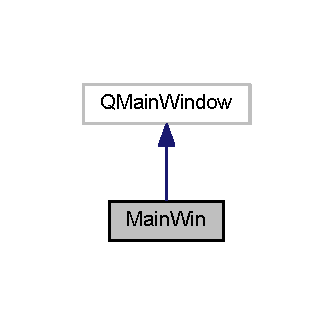
\includegraphics[width=160pt]{class_main_win__inherit__graph}
\end{center}
\end{figure}


Collaboration diagram for Main\-Win\-:\nopagebreak
\begin{figure}[H]
\begin{center}
\leavevmode
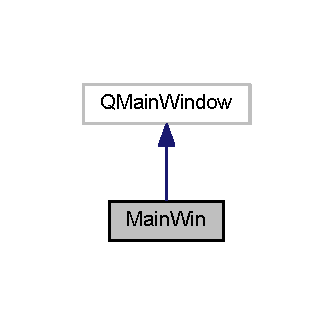
\includegraphics[width=160pt]{class_main_win__coll__graph}
\end{center}
\end{figure}
\subsection*{Public Member Functions}
\begin{DoxyCompactItemize}
\item 
\hypertarget{class_main_win_af05332e6fac4f7ab5c19b1a72aa7439d}{\hyperlink{class_main_win_af05332e6fac4f7ab5c19b1a72aa7439d}{Main\-Win} ()}\label{class_main_win_af05332e6fac4f7ab5c19b1a72aa7439d}

\begin{DoxyCompactList}\small\item\em Constructor. \end{DoxyCompactList}\item 
\hypertarget{class_main_win_a7068bb5ab02b75d4bbc78692388b9fb1}{\hyperlink{class_main_win_a7068bb5ab02b75d4bbc78692388b9fb1}{$\sim$\-Main\-Win} ()}\label{class_main_win_a7068bb5ab02b75d4bbc78692388b9fb1}

\begin{DoxyCompactList}\small\item\em Destructor. \end{DoxyCompactList}\item 
Q\-Size \hyperlink{class_main_win_af8f1854089c63efd6895ff536ad6ffc3}{size\-Hint} () const 
\begin{DoxyCompactList}\small\item\em Returns the desired size for when the window is created. \end{DoxyCompactList}\end{DoxyCompactItemize}
\subsection*{Protected Member Functions}
\begin{DoxyCompactItemize}
\item 
void \hyperlink{class_main_win_a06beabefe32c4e6514f76a07f1b63232}{close\-Event} (Q\-Close\-Event $\ast$event)
\begin{DoxyCompactList}\small\item\em Called when this window is closed\-: handles checking of log window. \end{DoxyCompactList}\end{DoxyCompactItemize}


\subsection{Detailed Description}
Application window class. 

Each \hyperlink{class_main_win}{Main\-Win} correcponds to exactly one currently open map document. If a new map document is created, it requires a new \hyperlink{class_main_win}{Main\-Win}. When the last \hyperlink{class_main_win}{Main\-Win} is closed, it will handle the closing of the log window if it is still open. 

\subsection{Member Function Documentation}
\hypertarget{class_main_win_a06beabefe32c4e6514f76a07f1b63232}{\index{Main\-Win@{Main\-Win}!close\-Event@{close\-Event}}
\index{close\-Event@{close\-Event}!MainWin@{Main\-Win}}
\subsubsection[{close\-Event}]{\setlength{\rightskip}{0pt plus 5cm}void Main\-Win\-::close\-Event (
\begin{DoxyParamCaption}
\item[{Q\-Close\-Event $\ast$}]{event}
\end{DoxyParamCaption}
)\hspace{0.3cm}{\ttfamily [protected]}}}\label{class_main_win_a06beabefe32c4e6514f76a07f1b63232}


Called when this window is closed\-: handles checking of log window. 


\begin{DoxyParams}{Parameters}
{\em event} & Close event. \\
\hline
\end{DoxyParams}
\hypertarget{class_main_win_af8f1854089c63efd6895ff536ad6ffc3}{\index{Main\-Win@{Main\-Win}!size\-Hint@{size\-Hint}}
\index{size\-Hint@{size\-Hint}!MainWin@{Main\-Win}}
\subsubsection[{size\-Hint}]{\setlength{\rightskip}{0pt plus 5cm}Q\-Size Main\-Win\-::size\-Hint (
\begin{DoxyParamCaption}
{}
\end{DoxyParamCaption}
) const\hspace{0.3cm}{\ttfamily [inline]}}}\label{class_main_win_af8f1854089c63efd6895ff536ad6ffc3}


Returns the desired size for when the window is created. 

\begin{DoxyReturn}{Returns}
Desired size. 
\end{DoxyReturn}


The documentation for this class was generated from the following files\-:\begin{DoxyCompactItemize}
\item 
app/\hyperlink{mainwin_8h}{mainwin.\-h}\item 
app/mainwin.\-cpp\end{DoxyCompactItemize}

\hypertarget{class_plugin_manager}{\section{Plugin\-Manager Class Reference}
\label{class_plugin_manager}\index{Plugin\-Manager@{Plugin\-Manager}}
}


Manages loading of plugins.  




{\ttfamily \#include $<$pluginmanager.\-h$>$}



Inheritance diagram for Plugin\-Manager\-:
\nopagebreak
\begin{figure}[H]
\begin{center}
\leavevmode
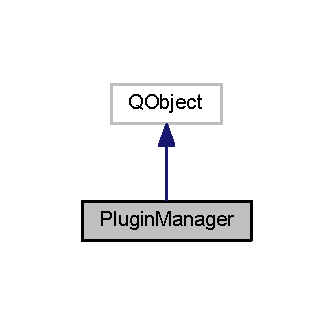
\includegraphics[width=160pt]{class_plugin_manager__inherit__graph}
\end{center}
\end{figure}


Collaboration diagram for Plugin\-Manager\-:
\nopagebreak
\begin{figure}[H]
\begin{center}
\leavevmode
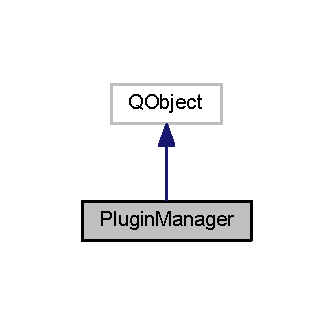
\includegraphics[width=160pt]{class_plugin_manager__coll__graph}
\end{center}
\end{figure}
\subsection*{Public Slots}
\begin{DoxyCompactItemize}
\item 
void \hyperlink{class_plugin_manager_a2e8795656b18a1ff483f2d7a4a6b7988}{Set\-Load\-Dir} (Q\-String dir)
\begin{DoxyCompactList}\small\item\em Sets the directory from which to load plugins. \end{DoxyCompactList}\end{DoxyCompactItemize}
\subsection*{Public Member Functions}
\begin{DoxyCompactItemize}
\item 
\hyperlink{class_plugin_manager_aac3752227a8bdae34eada08e6b80c3ce}{Plugin\-Manager} (Q\-Object $\ast$parent=0, Q\-String load\-Dir=\char`\"{}\char`\"{})
\begin{DoxyCompactList}\small\item\em Constructor. \end{DoxyCompactList}\item 
\hypertarget{class_plugin_manager_ab657302ef5af357907ae11ad817f5dfc}{\hyperlink{class_plugin_manager_ab657302ef5af357907ae11ad817f5dfc}{$\sim$\-Plugin\-Manager} ()}\label{class_plugin_manager_ab657302ef5af357907ae11ad817f5dfc}

\begin{DoxyCompactList}\small\item\em Destructor. \end{DoxyCompactList}\item 
Q\-List$<$ Q\-String $>$ \hyperlink{class_plugin_manager_a31f3817b1f01dac04059827dc0fe37f7}{Load\-Plugins} ()
\begin{DoxyCompactList}\small\item\em Loads plugins and returns a list of I\-Ds for those successfully loaded. \end{DoxyCompactList}\end{DoxyCompactItemize}
\subsection*{Protected Member Functions}
\begin{DoxyCompactItemize}
\item 
\hypertarget{class_plugin_manager_a7299c68a352c5fde51e803b32828b3da}{void \hyperlink{class_plugin_manager_a7299c68a352c5fde51e803b32828b3da}{Delete\-Plugin\-List} ()}\label{class_plugin_manager_a7299c68a352c5fde51e803b32828b3da}

\begin{DoxyCompactList}\small\item\em Destroys all plugins in the hash table. \end{DoxyCompactList}\item 
Q\-Dir \hyperlink{class_plugin_manager_a08a9b22dabdc191e7ce173c8fca93821}{Full\-Plugin\-Path} ()
\begin{DoxyCompactList}\small\item\em Generates full path from given plugin load directory. \end{DoxyCompactList}\end{DoxyCompactItemize}
\subsection*{Protected Attributes}
\begin{DoxyCompactItemize}
\item 
Q\-String \hyperlink{class_plugin_manager_ad76c45e41d41eac52be4ba19e4ae11fb}{m\-\_\-sz\-Load\-Dir}
\item 
Q\-Hash$<$ Q\-String, Q\-Object $\ast$ $>$ $\ast$ \hyperlink{class_plugin_manager_af65cae6069dfdb469aee42c4d2ec94d2}{m\-\_\-\-Plugin\-List}
\end{DoxyCompactItemize}


\subsection{Detailed Description}
Manages loading of plugins. 

\subsection{Constructor \& Destructor Documentation}
\hypertarget{class_plugin_manager_aac3752227a8bdae34eada08e6b80c3ce}{\index{Plugin\-Manager@{Plugin\-Manager}!Plugin\-Manager@{Plugin\-Manager}}
\index{Plugin\-Manager@{Plugin\-Manager}!PluginManager@{Plugin\-Manager}}
\subsubsection[{Plugin\-Manager}]{\setlength{\rightskip}{0pt plus 5cm}Plugin\-Manager\-::\-Plugin\-Manager (
\begin{DoxyParamCaption}
\item[{Q\-Object $\ast$}]{parent = {\ttfamily 0}, }
\item[{Q\-String}]{load\-Dir = {\ttfamily \char`\"{}\char`\"{}}}
\end{DoxyParamCaption}
)\hspace{0.3cm}{\ttfamily [explicit]}}}\label{class_plugin_manager_aac3752227a8bdae34eada08e6b80c3ce}


Constructor. 


\begin{DoxyParams}{Parameters}
{\em parent} & Parent object (usually N\-U\-L\-L). \\
\hline
{\em load\-Dir} & Directory from which to load plugins, relative to the application directory. \\
\hline
\end{DoxyParams}


\subsection{Member Function Documentation}
\hypertarget{class_plugin_manager_a08a9b22dabdc191e7ce173c8fca93821}{\index{Plugin\-Manager@{Plugin\-Manager}!Full\-Plugin\-Path@{Full\-Plugin\-Path}}
\index{Full\-Plugin\-Path@{Full\-Plugin\-Path}!PluginManager@{Plugin\-Manager}}
\subsubsection[{Full\-Plugin\-Path}]{\setlength{\rightskip}{0pt plus 5cm}Q\-Dir Plugin\-Manager\-::\-Full\-Plugin\-Path (
\begin{DoxyParamCaption}
{}
\end{DoxyParamCaption}
)\hspace{0.3cm}{\ttfamily [protected]}}}\label{class_plugin_manager_a08a9b22dabdc191e7ce173c8fca93821}


Generates full path from given plugin load directory. 

\begin{DoxyNote}{Note}
If the path does not exist, the returned path will be the application directory. 
\end{DoxyNote}
\begin{DoxyReturn}{Returns}
Full path of application and load directory. 
\end{DoxyReturn}
\hypertarget{class_plugin_manager_a31f3817b1f01dac04059827dc0fe37f7}{\index{Plugin\-Manager@{Plugin\-Manager}!Load\-Plugins@{Load\-Plugins}}
\index{Load\-Plugins@{Load\-Plugins}!PluginManager@{Plugin\-Manager}}
\subsubsection[{Load\-Plugins}]{\setlength{\rightskip}{0pt plus 5cm}Q\-List$<$ Q\-String $>$ Plugin\-Manager\-::\-Load\-Plugins (
\begin{DoxyParamCaption}
{}
\end{DoxyParamCaption}
)}}\label{class_plugin_manager_a31f3817b1f01dac04059827dc0fe37f7}


Loads plugins and returns a list of I\-Ds for those successfully loaded. 

\begin{DoxyReturn}{Returns}
List of successfully loaded plugins. 
\end{DoxyReturn}
\hypertarget{class_plugin_manager_a2e8795656b18a1ff483f2d7a4a6b7988}{\index{Plugin\-Manager@{Plugin\-Manager}!Set\-Load\-Dir@{Set\-Load\-Dir}}
\index{Set\-Load\-Dir@{Set\-Load\-Dir}!PluginManager@{Plugin\-Manager}}
\subsubsection[{Set\-Load\-Dir}]{\setlength{\rightskip}{0pt plus 5cm}void Plugin\-Manager\-::\-Set\-Load\-Dir (
\begin{DoxyParamCaption}
\item[{Q\-String}]{dir}
\end{DoxyParamCaption}
)\hspace{0.3cm}{\ttfamily [inline]}, {\ttfamily [slot]}}}\label{class_plugin_manager_a2e8795656b18a1ff483f2d7a4a6b7988}


Sets the directory from which to load plugins. 


\begin{DoxyParams}{Parameters}
{\em dir} & Directory path relative to the application directory. \\
\hline
\end{DoxyParams}


\subsection{Member Data Documentation}
\hypertarget{class_plugin_manager_af65cae6069dfdb469aee42c4d2ec94d2}{\index{Plugin\-Manager@{Plugin\-Manager}!m\-\_\-\-Plugin\-List@{m\-\_\-\-Plugin\-List}}
\index{m\-\_\-\-Plugin\-List@{m\-\_\-\-Plugin\-List}!PluginManager@{Plugin\-Manager}}
\subsubsection[{m\-\_\-\-Plugin\-List}]{\setlength{\rightskip}{0pt plus 5cm}Q\-Hash$<$Q\-String, Q\-Object$\ast$$>$$\ast$ Plugin\-Manager\-::m\-\_\-\-Plugin\-List\hspace{0.3cm}{\ttfamily [protected]}}}\label{class_plugin_manager_af65cae6069dfdb469aee42c4d2ec94d2}
List of all loaded plugins. \hypertarget{class_plugin_manager_ad76c45e41d41eac52be4ba19e4ae11fb}{\index{Plugin\-Manager@{Plugin\-Manager}!m\-\_\-sz\-Load\-Dir@{m\-\_\-sz\-Load\-Dir}}
\index{m\-\_\-sz\-Load\-Dir@{m\-\_\-sz\-Load\-Dir}!PluginManager@{Plugin\-Manager}}
\subsubsection[{m\-\_\-sz\-Load\-Dir}]{\setlength{\rightskip}{0pt plus 5cm}Q\-String Plugin\-Manager\-::m\-\_\-sz\-Load\-Dir\hspace{0.3cm}{\ttfamily [protected]}}}\label{class_plugin_manager_ad76c45e41d41eac52be4ba19e4ae11fb}
Path to load plugins from. 

The documentation for this class was generated from the following files\-:\begin{DoxyCompactItemize}
\item 
app/\hyperlink{pluginmanager_8h}{pluginmanager.\-h}\item 
app/pluginmanager.\-cpp\end{DoxyCompactItemize}

\hypertarget{class_string_property}{\section{String\-Property Class Reference}
\label{class_string_property}\index{String\-Property@{String\-Property}}
}


The \hyperlink{class_string_property}{String\-Property} class Class that handles string properties.  




{\ttfamily \#include $<$property.\-h$>$}



Inheritance diagram for String\-Property\-:
\nopagebreak
\begin{figure}[H]
\begin{center}
\leavevmode
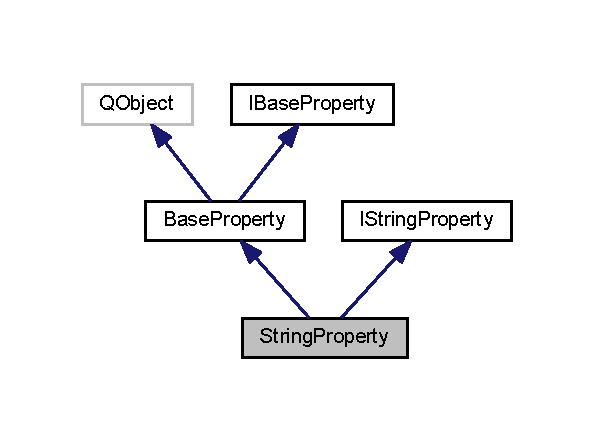
\includegraphics[width=285pt]{class_string_property__inherit__graph}
\end{center}
\end{figure}


Collaboration diagram for String\-Property\-:
\nopagebreak
\begin{figure}[H]
\begin{center}
\leavevmode
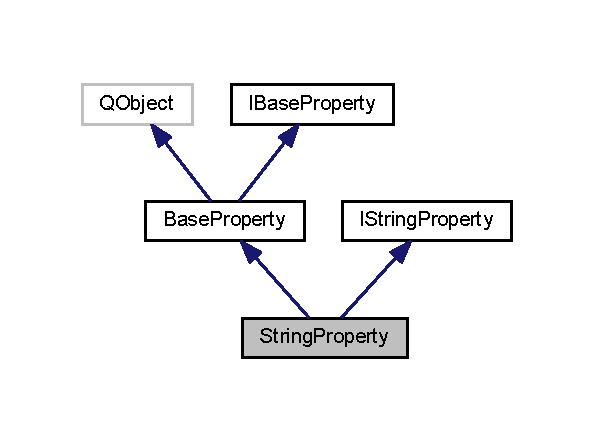
\includegraphics[width=285pt]{class_string_property__coll__graph}
\end{center}
\end{figure}
\subsection*{Public Member Functions}
\begin{DoxyCompactItemize}
\item 
\hyperlink{class_string_property_a587299d1879f0d70741a53afb895dce0}{String\-Property} (Q\-Object $\ast$parent=0, Q\-String key=\char`\"{}\char`\"{}, Q\-String value=\char`\"{}\char`\"{}, Q\-String comment=\char`\"{}\char`\"{})
\begin{DoxyCompactList}\small\item\em Constructor. Parameters not passed are initialised to safe null values. \end{DoxyCompactList}\item 
\hyperlink{class_w_string_property}{W\-String\-Property} $\ast$ \hyperlink{class_string_property_a3a9342b9b32b2ababdaec43cf3849b87}{slots\-For} () const 
\begin{DoxyCompactList}\small\item\em Returns the interface wrapper to allow binding to slots on this property. \end{DoxyCompactList}\item 
virtual \hyperlink{group___property_classes_ga38f1ccddda12c7cb50b868c9f789ee37}{Property\-\_\-t} \hyperlink{class_string_property_aa9a92e89f0076598d9651bc3269dbace}{get\-Property\-Type} () const 
\begin{DoxyCompactList}\small\item\em Returns the Property\-\_\-t to classify this property. \end{DoxyCompactList}\item 
virtual Q\-String \hyperlink{class_string_property_a7130232ef2d861bf098e25f47deb12cb}{get\-Value} (bool $\ast$success) const 
\begin{DoxyCompactList}\small\item\em Gets this property's value as \-\_\-type. \end{DoxyCompactList}\item 
virtual bool \hyperlink{class_string_property_aa080538ba6c8ed9cfde97781dfc416cc}{can\-Convert} () const 
\begin{DoxyCompactList}\small\item\em Returns whether or not the property's value can be successfully converted. \end{DoxyCompactList}\item 
virtual void \hyperlink{class_string_property_afebd41088d80724b87b2a1dcf41423ca}{set\-Value} (Q\-String value)
\begin{DoxyCompactList}\small\item\em Sets the property's value as \-\_\-type. \end{DoxyCompactList}\end{DoxyCompactItemize}
\subsection*{Additional Inherited Members}


\subsection{Detailed Description}
The \hyperlink{class_string_property}{String\-Property} class Class that handles string properties. 

\subsection{Constructor \& Destructor Documentation}
\hypertarget{class_string_property_a587299d1879f0d70741a53afb895dce0}{\index{String\-Property@{String\-Property}!String\-Property@{String\-Property}}
\index{String\-Property@{String\-Property}!StringProperty@{String\-Property}}
\subsubsection[{String\-Property}]{\setlength{\rightskip}{0pt plus 5cm}String\-Property\-::\-String\-Property (
\begin{DoxyParamCaption}
\item[{Q\-Object $\ast$}]{parent = {\ttfamily 0}, }
\item[{Q\-String}]{key = {\ttfamily \char`\"{}\char`\"{}}, }
\item[{Q\-String}]{value = {\ttfamily \char`\"{}\char`\"{}}, }
\item[{Q\-String}]{comment = {\ttfamily \char`\"{}\char`\"{}}}
\end{DoxyParamCaption}
)\hspace{0.3cm}{\ttfamily [explicit]}}}\label{class_string_property_a587299d1879f0d70741a53afb895dce0}


Constructor. Parameters not passed are initialised to safe null values. 


\begin{DoxyParams}{Parameters}
{\em parent} & Parent object for this property. \\
\hline
{\em key} & Property key (should be unique). \\
\hline
{\em value} & Property value. \\
\hline
{\em comment} & Optional string comment for when this property is written into a config file. \\
\hline
\end{DoxyParams}


\subsection{Member Function Documentation}
\hypertarget{class_string_property_aa080538ba6c8ed9cfde97781dfc416cc}{\index{String\-Property@{String\-Property}!can\-Convert@{can\-Convert}}
\index{can\-Convert@{can\-Convert}!StringProperty@{String\-Property}}
\subsubsection[{can\-Convert}]{\setlength{\rightskip}{0pt plus 5cm}bool String\-Property\-::can\-Convert (
\begin{DoxyParamCaption}
{}
\end{DoxyParamCaption}
) const\hspace{0.3cm}{\ttfamily [inline]}, {\ttfamily [virtual]}}}\label{class_string_property_aa080538ba6c8ed9cfde97781dfc416cc}


Returns whether or not the property's value can be successfully converted. 

\begin{DoxyReturn}{Returns}
True if conversion is possible, false otherwise. 
\end{DoxyReturn}


Implements \hyperlink{class_i_string_property_a2fcab392710db1ae140e394c1db6739e}{I\-String\-Property}.

\hypertarget{class_string_property_aa9a92e89f0076598d9651bc3269dbace}{\index{String\-Property@{String\-Property}!get\-Property\-Type@{get\-Property\-Type}}
\index{get\-Property\-Type@{get\-Property\-Type}!StringProperty@{String\-Property}}
\subsubsection[{get\-Property\-Type}]{\setlength{\rightskip}{0pt plus 5cm}virtual {\bf Property\-\_\-t} String\-Property\-::get\-Property\-Type (
\begin{DoxyParamCaption}
{}
\end{DoxyParamCaption}
) const\hspace{0.3cm}{\ttfamily [inline]}, {\ttfamily [virtual]}}}\label{class_string_property_aa9a92e89f0076598d9651bc3269dbace}


Returns the Property\-\_\-t to classify this property. 

\begin{DoxyReturn}{Returns}
Property\-\_\-t classifier. 
\end{DoxyReturn}


Reimplemented from \hyperlink{class_base_property_a85239fb7297edb01c3176e4ce1b11132}{Base\-Property}.

\hypertarget{class_string_property_a7130232ef2d861bf098e25f47deb12cb}{\index{String\-Property@{String\-Property}!get\-Value@{get\-Value}}
\index{get\-Value@{get\-Value}!StringProperty@{String\-Property}}
\subsubsection[{get\-Value}]{\setlength{\rightskip}{0pt plus 5cm}Q\-String String\-Property\-::get\-Value (
\begin{DoxyParamCaption}
\item[{bool $\ast$}]{success}
\end{DoxyParamCaption}
) const\hspace{0.3cm}{\ttfamily [inline]}, {\ttfamily [virtual]}}}\label{class_string_property_a7130232ef2d861bf098e25f47deb12cb}


Gets this property's value as \-\_\-type. 


\begin{DoxyParams}{Parameters}
{\em success} & True if conversion was successful, false otherwise. \\
\hline
\end{DoxyParams}
\begin{DoxyReturn}{Returns}
The property's value. 
\end{DoxyReturn}


Implements \hyperlink{class_i_string_property_a0dbe79993973e018510325120762504f}{I\-String\-Property}.

\hypertarget{class_string_property_afebd41088d80724b87b2a1dcf41423ca}{\index{String\-Property@{String\-Property}!set\-Value@{set\-Value}}
\index{set\-Value@{set\-Value}!StringProperty@{String\-Property}}
\subsubsection[{set\-Value}]{\setlength{\rightskip}{0pt plus 5cm}void String\-Property\-::set\-Value (
\begin{DoxyParamCaption}
\item[{Q\-String}]{value}
\end{DoxyParamCaption}
)\hspace{0.3cm}{\ttfamily [inline]}, {\ttfamily [virtual]}}}\label{class_string_property_afebd41088d80724b87b2a1dcf41423ca}


Sets the property's value as \-\_\-type. 


\begin{DoxyParams}{Parameters}
{\em value} & Value to set. \\
\hline
\end{DoxyParams}


Implements \hyperlink{class_i_string_property_a300b7403e9ce2929dabb5bb62d11142d}{I\-String\-Property}.

\hypertarget{class_string_property_a3a9342b9b32b2ababdaec43cf3849b87}{\index{String\-Property@{String\-Property}!slots\-For@{slots\-For}}
\index{slots\-For@{slots\-For}!StringProperty@{String\-Property}}
\subsubsection[{slots\-For}]{\setlength{\rightskip}{0pt plus 5cm}{\bf W\-String\-Property}$\ast$ String\-Property\-::slots\-For (
\begin{DoxyParamCaption}
{}
\end{DoxyParamCaption}
) const\hspace{0.3cm}{\ttfamily [inline]}}}\label{class_string_property_a3a9342b9b32b2ababdaec43cf3849b87}


Returns the interface wrapper to allow binding to slots on this property. 

\begin{DoxyReturn}{Returns}
\hyperlink{class_w_string_property}{W\-String\-Property} interface wrapper. 
\end{DoxyReturn}


The documentation for this class was generated from the following files\-:\begin{DoxyCompactItemize}
\item 
app/\hyperlink{property_8h}{property.\-h}\item 
app/property.\-cpp\end{DoxyCompactItemize}

\hypertarget{class_u_int_property}{\section{U\-Int\-Property Class Reference}
\label{class_u_int_property}\index{U\-Int\-Property@{U\-Int\-Property}}
}


M\-A\-C\-R\-O P\-R\-O\-P\-E\-R\-T\-Y F\-O\-R uint .  




{\ttfamily \#include $<$property.\-h$>$}



Inheritance diagram for U\-Int\-Property\-:
\nopagebreak
\begin{figure}[H]
\begin{center}
\leavevmode
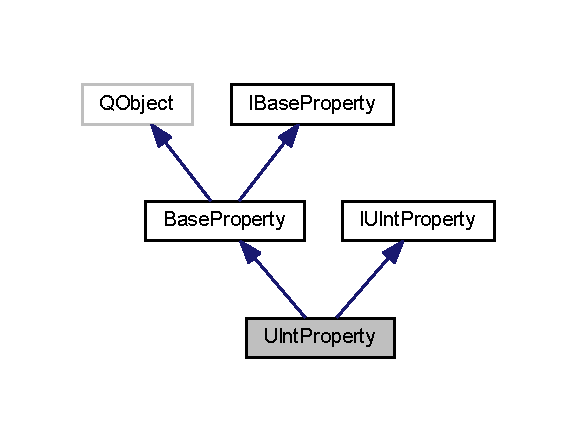
\includegraphics[width=277pt]{class_u_int_property__inherit__graph}
\end{center}
\end{figure}


Collaboration diagram for U\-Int\-Property\-:
\nopagebreak
\begin{figure}[H]
\begin{center}
\leavevmode
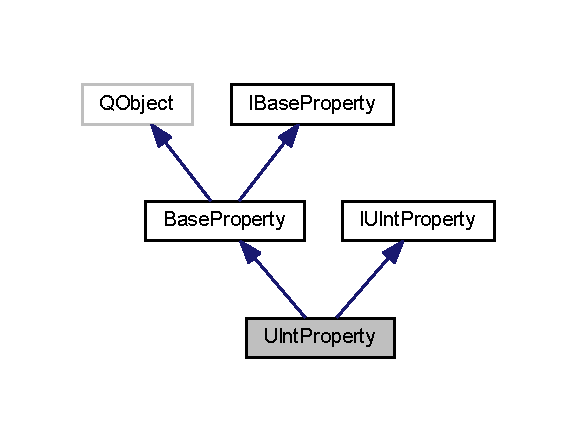
\includegraphics[width=277pt]{class_u_int_property__coll__graph}
\end{center}
\end{figure}
\subsection*{Public Member Functions}
\begin{DoxyCompactItemize}
\item 
\hyperlink{class_u_int_property_a6f8d978c3fe5ba65656323690a2c580b}{U\-Int\-Property} (Q\-Object $\ast$parent=0, Q\-String key=\char`\"{}\char`\"{}, uint value=0, Q\-String comment=\char`\"{}\char`\"{})
\begin{DoxyCompactList}\small\item\em Constructor. Parameters not passed are initialised to safe null values. \end{DoxyCompactList}\item 
virtual \hyperlink{group___property_classes_ga38f1ccddda12c7cb50b868c9f789ee37}{Property\-\_\-t} \hyperlink{class_u_int_property_a3c42cb68115d9ac7fec4887de32d867e}{get\-Property\-Type} () const 
\begin{DoxyCompactList}\small\item\em Returns the Property\-\_\-t to classify this property. \end{DoxyCompactList}\item 
virtual uint \hyperlink{class_u_int_property_a9f1ce8733358de31a642990168f3f61d}{get\-Value} (bool $\ast$success) const 
\begin{DoxyCompactList}\small\item\em Gets this property's value as uint . \end{DoxyCompactList}\item 
virtual bool \hyperlink{class_u_int_property_a3f9986864fcd8cbfefd69245dc7aadfe}{can\-Convert} () const 
\begin{DoxyCompactList}\small\item\em Returns whether or not the property's value can be successfully converted. \end{DoxyCompactList}\item 
virtual void \hyperlink{class_u_int_property_a074ce84b6839d2451a3abee9da289198}{set\-Value} (uint value)
\begin{DoxyCompactList}\small\item\em Sets the property's value as uint . \end{DoxyCompactList}\item 
virtual \hyperlink{class_w_u_int_property}{W\-U\-Int\-Property} $\ast$ \hyperlink{class_u_int_property_a8625bb395e98f5db5b4963a40d7ced32}{slots\-For} () const 
\begin{DoxyCompactList}\small\item\em Returns the interface wrapper to allow binding to slots on this property. \end{DoxyCompactList}\end{DoxyCompactItemize}
\subsection*{Additional Inherited Members}


\subsection{Detailed Description}
M\-A\-C\-R\-O P\-R\-O\-P\-E\-R\-T\-Y F\-O\-R uint . 

Property that handles data of type uint . 

\subsection{Constructor \& Destructor Documentation}
\hypertarget{class_u_int_property_a6f8d978c3fe5ba65656323690a2c580b}{\index{U\-Int\-Property@{U\-Int\-Property}!U\-Int\-Property@{U\-Int\-Property}}
\index{U\-Int\-Property@{U\-Int\-Property}!UIntProperty@{U\-Int\-Property}}
\subsubsection[{U\-Int\-Property}]{\setlength{\rightskip}{0pt plus 5cm}U\-Int\-Property\-::\-U\-Int\-Property (
\begin{DoxyParamCaption}
\item[{Q\-Object $\ast$}]{parent = {\ttfamily 0}, }
\item[{Q\-String}]{key = {\ttfamily \char`\"{}\char`\"{}}, }
\item[{uint}]{value = {\ttfamily 0}, }
\item[{Q\-String}]{comment = {\ttfamily \char`\"{}\char`\"{}}}
\end{DoxyParamCaption}
)\hspace{0.3cm}{\ttfamily [explicit]}}}\label{class_u_int_property_a6f8d978c3fe5ba65656323690a2c580b}


Constructor. Parameters not passed are initialised to safe null values. 


\begin{DoxyParams}{Parameters}
{\em parent} & Parent object for this property.\\
\hline
{\em key} & Property key (should be unique).\\
\hline
{\em value} & Property value of type uint .\\
\hline
{\em comment} & Optional string comment for when this property is written into a config file. \\
\hline
\end{DoxyParams}


\subsection{Member Function Documentation}
\hypertarget{class_u_int_property_a3f9986864fcd8cbfefd69245dc7aadfe}{\index{U\-Int\-Property@{U\-Int\-Property}!can\-Convert@{can\-Convert}}
\index{can\-Convert@{can\-Convert}!UIntProperty@{U\-Int\-Property}}
\subsubsection[{can\-Convert}]{\setlength{\rightskip}{0pt plus 5cm}bool U\-Int\-Property\-::can\-Convert (
\begin{DoxyParamCaption}
{}
\end{DoxyParamCaption}
) const\hspace{0.3cm}{\ttfamily [virtual]}}}\label{class_u_int_property_a3f9986864fcd8cbfefd69245dc7aadfe}


Returns whether or not the property's value can be successfully converted. 

\begin{DoxyReturn}{Returns}
True if conversion is possible, false otherwise. 
\end{DoxyReturn}


Implements \hyperlink{class_i_u_int_property_a4fa6fa9ef5663109772bf51123323c87}{I\-U\-Int\-Property}.

\hypertarget{class_u_int_property_a3c42cb68115d9ac7fec4887de32d867e}{\index{U\-Int\-Property@{U\-Int\-Property}!get\-Property\-Type@{get\-Property\-Type}}
\index{get\-Property\-Type@{get\-Property\-Type}!UIntProperty@{U\-Int\-Property}}
\subsubsection[{get\-Property\-Type}]{\setlength{\rightskip}{0pt plus 5cm}virtual {\bf Property\-\_\-t} U\-Int\-Property\-::get\-Property\-Type (
\begin{DoxyParamCaption}
{}
\end{DoxyParamCaption}
) const\hspace{0.3cm}{\ttfamily [inline]}, {\ttfamily [virtual]}}}\label{class_u_int_property_a3c42cb68115d9ac7fec4887de32d867e}


Returns the Property\-\_\-t to classify this property. 

\begin{DoxyReturn}{Returns}
Property\-\_\-t classifier. 
\end{DoxyReturn}


Implements \hyperlink{class_i_u_int_property_a64bce0a1e93666424d3252e78216fa33}{I\-U\-Int\-Property}.

\hypertarget{class_u_int_property_a9f1ce8733358de31a642990168f3f61d}{\index{U\-Int\-Property@{U\-Int\-Property}!get\-Value@{get\-Value}}
\index{get\-Value@{get\-Value}!UIntProperty@{U\-Int\-Property}}
\subsubsection[{get\-Value}]{\setlength{\rightskip}{0pt plus 5cm}uint U\-Int\-Property\-::get\-Value (
\begin{DoxyParamCaption}
\item[{bool $\ast$}]{success}
\end{DoxyParamCaption}
) const\hspace{0.3cm}{\ttfamily [virtual]}}}\label{class_u_int_property_a9f1ce8733358de31a642990168f3f61d}


Gets this property's value as uint . 


\begin{DoxyParams}{Parameters}
{\em success} & True if conversion was successful, false otherwise.\\
\hline
\end{DoxyParams}
\begin{DoxyReturn}{Returns}
The property's value. 
\end{DoxyReturn}


Implements \hyperlink{class_i_u_int_property_af3c17d292a74241f1d80b10be434edde}{I\-U\-Int\-Property}.

\hypertarget{class_u_int_property_a074ce84b6839d2451a3abee9da289198}{\index{U\-Int\-Property@{U\-Int\-Property}!set\-Value@{set\-Value}}
\index{set\-Value@{set\-Value}!UIntProperty@{U\-Int\-Property}}
\subsubsection[{set\-Value}]{\setlength{\rightskip}{0pt plus 5cm}void U\-Int\-Property\-::set\-Value (
\begin{DoxyParamCaption}
\item[{uint}]{value}
\end{DoxyParamCaption}
)\hspace{0.3cm}{\ttfamily [virtual]}}}\label{class_u_int_property_a074ce84b6839d2451a3abee9da289198}


Sets the property's value as uint . 


\begin{DoxyParams}{Parameters}
{\em value} & Value to set. \\
\hline
\end{DoxyParams}


Implements \hyperlink{class_i_u_int_property_a2344d640892a4c3529bcca63c4c2531c}{I\-U\-Int\-Property}.

\hypertarget{class_u_int_property_a8625bb395e98f5db5b4963a40d7ced32}{\index{U\-Int\-Property@{U\-Int\-Property}!slots\-For@{slots\-For}}
\index{slots\-For@{slots\-For}!UIntProperty@{U\-Int\-Property}}
\subsubsection[{slots\-For}]{\setlength{\rightskip}{0pt plus 5cm}virtual {\bf W\-U\-Int\-Property}$\ast$ U\-Int\-Property\-::slots\-For (
\begin{DoxyParamCaption}
{}
\end{DoxyParamCaption}
) const\hspace{0.3cm}{\ttfamily [inline]}, {\ttfamily [virtual]}}}\label{class_u_int_property_a8625bb395e98f5db5b4963a40d7ced32}


Returns the interface wrapper to allow binding to slots on this property. 

\begin{DoxyReturn}{Returns}
\hyperlink{class_w_u_int_property}{W\-U\-Int\-Property} interface wrapper. 
\end{DoxyReturn}


The documentation for this class was generated from the following files\-:\begin{DoxyCompactItemize}
\item 
app/\hyperlink{property_8h}{property.\-h}\item 
app/property.\-cpp\end{DoxyCompactItemize}

\hypertarget{class_u_long_long_property}{\section{U\-Long\-Long\-Property Class Reference}
\label{class_u_long_long_property}\index{U\-Long\-Long\-Property@{U\-Long\-Long\-Property}}
}


M\-A\-C\-R\-O P\-R\-O\-P\-E\-R\-T\-Y F\-O\-R qulonglong .  




{\ttfamily \#include $<$property.\-h$>$}



Inheritance diagram for U\-Long\-Long\-Property\-:
\nopagebreak
\begin{figure}[H]
\begin{center}
\leavevmode
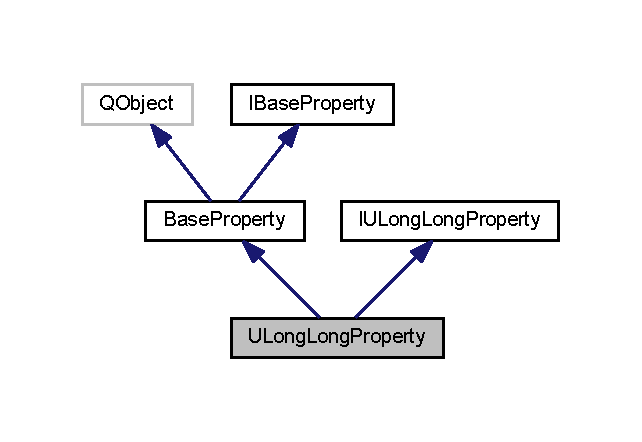
\includegraphics[width=308pt]{class_u_long_long_property__inherit__graph}
\end{center}
\end{figure}


Collaboration diagram for U\-Long\-Long\-Property\-:
\nopagebreak
\begin{figure}[H]
\begin{center}
\leavevmode
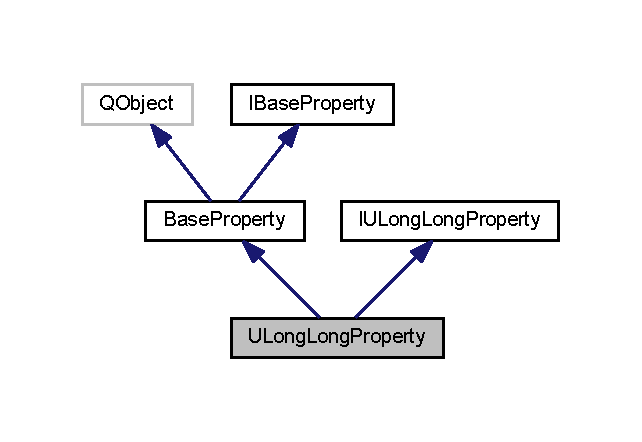
\includegraphics[width=308pt]{class_u_long_long_property__coll__graph}
\end{center}
\end{figure}
\subsection*{Public Member Functions}
\begin{DoxyCompactItemize}
\item 
\hyperlink{class_u_long_long_property_a2e62bdd765cd03324aa8abd4c84fb97a}{U\-Long\-Long\-Property} (Q\-Object $\ast$parent=0, Q\-String key=\char`\"{}\char`\"{}, qulonglong value=0, Q\-String comment=\char`\"{}\char`\"{})
\begin{DoxyCompactList}\small\item\em Constructor. Parameters not passed are initialised to safe null values. \end{DoxyCompactList}\item 
virtual \hyperlink{group___property_classes_ga38f1ccddda12c7cb50b868c9f789ee37}{Property\-\_\-t} \hyperlink{class_u_long_long_property_aaad8c3be9d1037f10e7bcd0713a404a9}{get\-Property\-Type} () const 
\begin{DoxyCompactList}\small\item\em Returns the Property\-\_\-t to classify this property. \end{DoxyCompactList}\item 
virtual bool \hyperlink{class_u_long_long_property_a501c2e699537199ef93ba3c765d3c310}{pass\-To} (\hyperlink{class_property_variant}{Property\-Variant} $\ast$variant)
\begin{DoxyCompactList}\small\item\em Passes the property's value to the variant. \end{DoxyCompactList}\item 
virtual qulonglong \hyperlink{class_u_long_long_property_ac2dadcd92de6e92c58620ebfd1e50b66}{get\-Value} (bool $\ast$success) const 
\begin{DoxyCompactList}\small\item\em Gets this property's value as qulonglong . \end{DoxyCompactList}\item 
virtual bool \hyperlink{class_u_long_long_property_a9b670e3778650e496146c24ac133c136}{can\-Convert} () const 
\begin{DoxyCompactList}\small\item\em Returns whether or not the property's value can be successfully converted. \end{DoxyCompactList}\item 
virtual void \hyperlink{class_u_long_long_property_abb1dcbdd5327e7cd261df653dadcc2c9}{set\-Value} (qulonglong value)
\begin{DoxyCompactList}\small\item\em Sets the property's value as qulonglong . \end{DoxyCompactList}\item 
virtual \hyperlink{class_w_u_long_long_property}{W\-U\-Long\-Long\-Property} $\ast$ \hyperlink{class_u_long_long_property_a17ca304df37d8fa3b78e9e685e627999}{slots\-For} () const 
\begin{DoxyCompactList}\small\item\em Returns the interface wrapper to allow binding to slots on this property. \end{DoxyCompactList}\end{DoxyCompactItemize}
\subsection*{Additional Inherited Members}


\subsection{Detailed Description}
M\-A\-C\-R\-O P\-R\-O\-P\-E\-R\-T\-Y F\-O\-R qulonglong . 

Property that handles data of type qulonglong . 

\subsection{Constructor \& Destructor Documentation}
\hypertarget{class_u_long_long_property_a2e62bdd765cd03324aa8abd4c84fb97a}{\index{U\-Long\-Long\-Property@{U\-Long\-Long\-Property}!U\-Long\-Long\-Property@{U\-Long\-Long\-Property}}
\index{U\-Long\-Long\-Property@{U\-Long\-Long\-Property}!ULongLongProperty@{U\-Long\-Long\-Property}}
\subsubsection[{U\-Long\-Long\-Property}]{\setlength{\rightskip}{0pt plus 5cm}U\-Long\-Long\-Property\-::\-U\-Long\-Long\-Property (
\begin{DoxyParamCaption}
\item[{Q\-Object $\ast$}]{parent = {\ttfamily 0}, }
\item[{Q\-String}]{key = {\ttfamily \char`\"{}\char`\"{}}, }
\item[{qulonglong}]{value = {\ttfamily 0}, }
\item[{Q\-String}]{comment = {\ttfamily \char`\"{}\char`\"{}}}
\end{DoxyParamCaption}
)\hspace{0.3cm}{\ttfamily [explicit]}}}\label{class_u_long_long_property_a2e62bdd765cd03324aa8abd4c84fb97a}


Constructor. Parameters not passed are initialised to safe null values. 


\begin{DoxyParams}{Parameters}
{\em parent} & Parent object for this property.\\
\hline
{\em key} & Property key (should be unique).\\
\hline
{\em value} & Property value of type qulonglong .\\
\hline
{\em comment} & Optional string comment for when this property is written into a config file. \\
\hline
\end{DoxyParams}


\subsection{Member Function Documentation}
\hypertarget{class_u_long_long_property_a9b670e3778650e496146c24ac133c136}{\index{U\-Long\-Long\-Property@{U\-Long\-Long\-Property}!can\-Convert@{can\-Convert}}
\index{can\-Convert@{can\-Convert}!ULongLongProperty@{U\-Long\-Long\-Property}}
\subsubsection[{can\-Convert}]{\setlength{\rightskip}{0pt plus 5cm}bool U\-Long\-Long\-Property\-::can\-Convert (
\begin{DoxyParamCaption}
{}
\end{DoxyParamCaption}
) const\hspace{0.3cm}{\ttfamily [virtual]}}}\label{class_u_long_long_property_a9b670e3778650e496146c24ac133c136}


Returns whether or not the property's value can be successfully converted. 

\begin{DoxyReturn}{Returns}
True if conversion is possible, false otherwise. 
\end{DoxyReturn}


Implements \hyperlink{class_i_u_long_long_property_a905e766d258ebf63ed683a32aa2427a0}{I\-U\-Long\-Long\-Property}.

\hypertarget{class_u_long_long_property_aaad8c3be9d1037f10e7bcd0713a404a9}{\index{U\-Long\-Long\-Property@{U\-Long\-Long\-Property}!get\-Property\-Type@{get\-Property\-Type}}
\index{get\-Property\-Type@{get\-Property\-Type}!ULongLongProperty@{U\-Long\-Long\-Property}}
\subsubsection[{get\-Property\-Type}]{\setlength{\rightskip}{0pt plus 5cm}virtual {\bf Property\-\_\-t} U\-Long\-Long\-Property\-::get\-Property\-Type (
\begin{DoxyParamCaption}
{}
\end{DoxyParamCaption}
) const\hspace{0.3cm}{\ttfamily [inline]}, {\ttfamily [virtual]}}}\label{class_u_long_long_property_aaad8c3be9d1037f10e7bcd0713a404a9}


Returns the Property\-\_\-t to classify this property. 

\begin{DoxyReturn}{Returns}
Property\-\_\-t classifier. 
\end{DoxyReturn}


Reimplemented from \hyperlink{class_base_property_a85239fb7297edb01c3176e4ce1b11132}{Base\-Property}.

\hypertarget{class_u_long_long_property_ac2dadcd92de6e92c58620ebfd1e50b66}{\index{U\-Long\-Long\-Property@{U\-Long\-Long\-Property}!get\-Value@{get\-Value}}
\index{get\-Value@{get\-Value}!ULongLongProperty@{U\-Long\-Long\-Property}}
\subsubsection[{get\-Value}]{\setlength{\rightskip}{0pt plus 5cm}qulonglong U\-Long\-Long\-Property\-::get\-Value (
\begin{DoxyParamCaption}
\item[{bool $\ast$}]{success}
\end{DoxyParamCaption}
) const\hspace{0.3cm}{\ttfamily [virtual]}}}\label{class_u_long_long_property_ac2dadcd92de6e92c58620ebfd1e50b66}


Gets this property's value as qulonglong . 


\begin{DoxyParams}{Parameters}
{\em success} & True if conversion was successful, false otherwise.\\
\hline
\end{DoxyParams}
\begin{DoxyReturn}{Returns}
The property's value. 
\end{DoxyReturn}


Implements \hyperlink{class_i_u_long_long_property_acddc945a90cac8fa5921a9be25aaed13}{I\-U\-Long\-Long\-Property}.

\hypertarget{class_u_long_long_property_a501c2e699537199ef93ba3c765d3c310}{\index{U\-Long\-Long\-Property@{U\-Long\-Long\-Property}!pass\-To@{pass\-To}}
\index{pass\-To@{pass\-To}!ULongLongProperty@{U\-Long\-Long\-Property}}
\subsubsection[{pass\-To}]{\setlength{\rightskip}{0pt plus 5cm}bool U\-Long\-Long\-Property\-::pass\-To (
\begin{DoxyParamCaption}
\item[{{\bf Property\-Variant} $\ast$}]{variant}
\end{DoxyParamCaption}
)\hspace{0.3cm}{\ttfamily [virtual]}}}\label{class_u_long_long_property_a501c2e699537199ef93ba3c765d3c310}


Passes the property's value to the variant. 


\begin{DoxyParams}{Parameters}
{\em variant} & Variant to pass to.\\
\hline
\end{DoxyParams}
\begin{DoxyReturn}{Returns}
True if conversion succeeded, false otherwise.
\end{DoxyReturn}

\begin{DoxyParams}{Parameters}
{\em variant} & Variant to pass to. \\
\hline
\end{DoxyParams}


Implements \hyperlink{class_i_u_long_long_property_afa78a1d7b4839a6af9c8e84fe61fb969}{I\-U\-Long\-Long\-Property}.

\hypertarget{class_u_long_long_property_abb1dcbdd5327e7cd261df653dadcc2c9}{\index{U\-Long\-Long\-Property@{U\-Long\-Long\-Property}!set\-Value@{set\-Value}}
\index{set\-Value@{set\-Value}!ULongLongProperty@{U\-Long\-Long\-Property}}
\subsubsection[{set\-Value}]{\setlength{\rightskip}{0pt plus 5cm}void U\-Long\-Long\-Property\-::set\-Value (
\begin{DoxyParamCaption}
\item[{qulonglong}]{value}
\end{DoxyParamCaption}
)\hspace{0.3cm}{\ttfamily [virtual]}}}\label{class_u_long_long_property_abb1dcbdd5327e7cd261df653dadcc2c9}


Sets the property's value as qulonglong . 


\begin{DoxyParams}{Parameters}
{\em value} & Value to set. \\
\hline
\end{DoxyParams}


Implements \hyperlink{class_i_u_long_long_property_a59001a53d5cfdc3933038398fbeca269}{I\-U\-Long\-Long\-Property}.

\hypertarget{class_u_long_long_property_a17ca304df37d8fa3b78e9e685e627999}{\index{U\-Long\-Long\-Property@{U\-Long\-Long\-Property}!slots\-For@{slots\-For}}
\index{slots\-For@{slots\-For}!ULongLongProperty@{U\-Long\-Long\-Property}}
\subsubsection[{slots\-For}]{\setlength{\rightskip}{0pt plus 5cm}virtual {\bf W\-U\-Long\-Long\-Property}$\ast$ U\-Long\-Long\-Property\-::slots\-For (
\begin{DoxyParamCaption}
{}
\end{DoxyParamCaption}
) const\hspace{0.3cm}{\ttfamily [inline]}, {\ttfamily [virtual]}}}\label{class_u_long_long_property_a17ca304df37d8fa3b78e9e685e627999}


Returns the interface wrapper to allow binding to slots on this property. 

\begin{DoxyReturn}{Returns}
\hyperlink{class_w_u_long_long_property}{W\-U\-Long\-Long\-Property} interface wrapper. 
\end{DoxyReturn}


The documentation for this class was generated from the following files\-:\begin{DoxyCompactItemize}
\item 
app/\hyperlink{property_8h}{property.\-h}\item 
app/property.\-cpp\end{DoxyCompactItemize}

\hypertarget{class_u_long_property}{\section{U\-Long\-Property Class Reference}
\label{class_u_long_property}\index{U\-Long\-Property@{U\-Long\-Property}}
}


M\-A\-C\-R\-O P\-R\-O\-P\-E\-R\-T\-Y F\-O\-R ulong .  




{\ttfamily \#include $<$property.\-h$>$}



Inheritance diagram for U\-Long\-Property\-:
\nopagebreak
\begin{figure}[H]
\begin{center}
\leavevmode
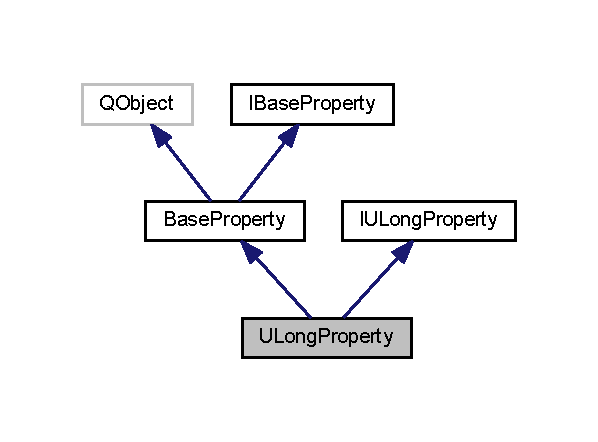
\includegraphics[width=287pt]{class_u_long_property__inherit__graph}
\end{center}
\end{figure}


Collaboration diagram for U\-Long\-Property\-:
\nopagebreak
\begin{figure}[H]
\begin{center}
\leavevmode
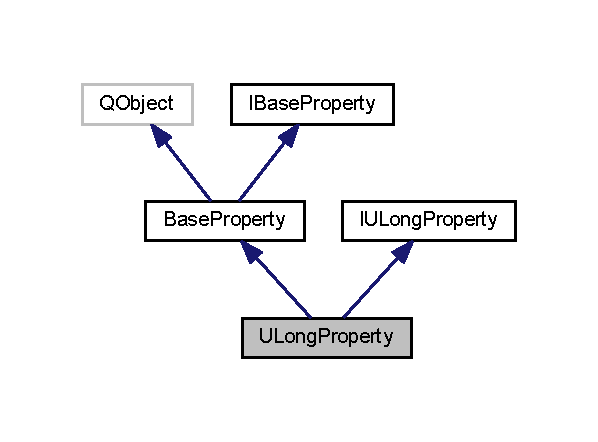
\includegraphics[width=287pt]{class_u_long_property__coll__graph}
\end{center}
\end{figure}
\subsection*{Public Member Functions}
\begin{DoxyCompactItemize}
\item 
\hyperlink{class_u_long_property_ac844158e013ca84c63b7bb434aa4ed4b}{U\-Long\-Property} (Q\-Object $\ast$parent=0, Q\-String key=\char`\"{}\char`\"{}, ulong value=0, Q\-String comment=\char`\"{}\char`\"{})
\begin{DoxyCompactList}\small\item\em Constructor. Parameters not passed are initialised to safe null values. \end{DoxyCompactList}\item 
virtual \hyperlink{group___property_classes_ga38f1ccddda12c7cb50b868c9f789ee37}{Property\-\_\-t} \hyperlink{class_u_long_property_aab8927e988f483d6334ba1ccffeeda99}{get\-Property\-Type} () const 
\begin{DoxyCompactList}\small\item\em Returns the Property\-\_\-t to classify this property. \end{DoxyCompactList}\item 
virtual bool \hyperlink{class_u_long_property_a08f952e4db14c65d472d4961dab9ac0c}{pass\-To} (\hyperlink{class_property_variant}{Property\-Variant} $\ast$variant)
\begin{DoxyCompactList}\small\item\em Passes the property's value to the variant. \end{DoxyCompactList}\item 
virtual ulong \hyperlink{class_u_long_property_a2d0ab1518fe88b2201b98dd5adf7f0a2}{get\-Value} (bool $\ast$success) const 
\begin{DoxyCompactList}\small\item\em Gets this property's value as ulong . \end{DoxyCompactList}\item 
virtual bool \hyperlink{class_u_long_property_a1ceb817d2b4fad531e3a893ad1b33273}{can\-Convert} () const 
\begin{DoxyCompactList}\small\item\em Returns whether or not the property's value can be successfully converted. \end{DoxyCompactList}\item 
virtual void \hyperlink{class_u_long_property_ac52a81a11a65723ab008ba066be522f3}{set\-Value} (ulong value)
\begin{DoxyCompactList}\small\item\em Sets the property's value as ulong . \end{DoxyCompactList}\item 
virtual \hyperlink{class_w_u_long_property}{W\-U\-Long\-Property} $\ast$ \hyperlink{class_u_long_property_a9c7a625deeba3f906ae2cb415a9eddfb}{slots\-For} () const 
\begin{DoxyCompactList}\small\item\em Returns the interface wrapper to allow binding to slots on this property. \end{DoxyCompactList}\end{DoxyCompactItemize}
\subsection*{Additional Inherited Members}


\subsection{Detailed Description}
M\-A\-C\-R\-O P\-R\-O\-P\-E\-R\-T\-Y F\-O\-R ulong . 

Property that handles data of type ulong . 

\subsection{Constructor \& Destructor Documentation}
\hypertarget{class_u_long_property_ac844158e013ca84c63b7bb434aa4ed4b}{\index{U\-Long\-Property@{U\-Long\-Property}!U\-Long\-Property@{U\-Long\-Property}}
\index{U\-Long\-Property@{U\-Long\-Property}!ULongProperty@{U\-Long\-Property}}
\subsubsection[{U\-Long\-Property}]{\setlength{\rightskip}{0pt plus 5cm}U\-Long\-Property\-::\-U\-Long\-Property (
\begin{DoxyParamCaption}
\item[{Q\-Object $\ast$}]{parent = {\ttfamily 0}, }
\item[{Q\-String}]{key = {\ttfamily \char`\"{}\char`\"{}}, }
\item[{ulong}]{value = {\ttfamily 0}, }
\item[{Q\-String}]{comment = {\ttfamily \char`\"{}\char`\"{}}}
\end{DoxyParamCaption}
)\hspace{0.3cm}{\ttfamily [explicit]}}}\label{class_u_long_property_ac844158e013ca84c63b7bb434aa4ed4b}


Constructor. Parameters not passed are initialised to safe null values. 


\begin{DoxyParams}{Parameters}
{\em parent} & Parent object for this property.\\
\hline
{\em key} & Property key (should be unique).\\
\hline
{\em value} & Property value of type ulong .\\
\hline
{\em comment} & Optional string comment for when this property is written into a config file. \\
\hline
\end{DoxyParams}


\subsection{Member Function Documentation}
\hypertarget{class_u_long_property_a1ceb817d2b4fad531e3a893ad1b33273}{\index{U\-Long\-Property@{U\-Long\-Property}!can\-Convert@{can\-Convert}}
\index{can\-Convert@{can\-Convert}!ULongProperty@{U\-Long\-Property}}
\subsubsection[{can\-Convert}]{\setlength{\rightskip}{0pt plus 5cm}bool U\-Long\-Property\-::can\-Convert (
\begin{DoxyParamCaption}
{}
\end{DoxyParamCaption}
) const\hspace{0.3cm}{\ttfamily [virtual]}}}\label{class_u_long_property_a1ceb817d2b4fad531e3a893ad1b33273}


Returns whether or not the property's value can be successfully converted. 

\begin{DoxyReturn}{Returns}
True if conversion is possible, false otherwise. 
\end{DoxyReturn}


Implements \hyperlink{class_i_u_long_property_ad63c658df7494298fd8a0ab41623a184}{I\-U\-Long\-Property}.

\hypertarget{class_u_long_property_aab8927e988f483d6334ba1ccffeeda99}{\index{U\-Long\-Property@{U\-Long\-Property}!get\-Property\-Type@{get\-Property\-Type}}
\index{get\-Property\-Type@{get\-Property\-Type}!ULongProperty@{U\-Long\-Property}}
\subsubsection[{get\-Property\-Type}]{\setlength{\rightskip}{0pt plus 5cm}virtual {\bf Property\-\_\-t} U\-Long\-Property\-::get\-Property\-Type (
\begin{DoxyParamCaption}
{}
\end{DoxyParamCaption}
) const\hspace{0.3cm}{\ttfamily [inline]}, {\ttfamily [virtual]}}}\label{class_u_long_property_aab8927e988f483d6334ba1ccffeeda99}


Returns the Property\-\_\-t to classify this property. 

\begin{DoxyReturn}{Returns}
Property\-\_\-t classifier. 
\end{DoxyReturn}


Reimplemented from \hyperlink{class_base_property_a85239fb7297edb01c3176e4ce1b11132}{Base\-Property}.

\hypertarget{class_u_long_property_a2d0ab1518fe88b2201b98dd5adf7f0a2}{\index{U\-Long\-Property@{U\-Long\-Property}!get\-Value@{get\-Value}}
\index{get\-Value@{get\-Value}!ULongProperty@{U\-Long\-Property}}
\subsubsection[{get\-Value}]{\setlength{\rightskip}{0pt plus 5cm}ulong U\-Long\-Property\-::get\-Value (
\begin{DoxyParamCaption}
\item[{bool $\ast$}]{success}
\end{DoxyParamCaption}
) const\hspace{0.3cm}{\ttfamily [virtual]}}}\label{class_u_long_property_a2d0ab1518fe88b2201b98dd5adf7f0a2}


Gets this property's value as ulong . 


\begin{DoxyParams}{Parameters}
{\em success} & True if conversion was successful, false otherwise.\\
\hline
\end{DoxyParams}
\begin{DoxyReturn}{Returns}
The property's value. 
\end{DoxyReturn}


Implements \hyperlink{class_i_u_long_property_a620e0d9b7260d93ee9e5a55c5c648f92}{I\-U\-Long\-Property}.

\hypertarget{class_u_long_property_a08f952e4db14c65d472d4961dab9ac0c}{\index{U\-Long\-Property@{U\-Long\-Property}!pass\-To@{pass\-To}}
\index{pass\-To@{pass\-To}!ULongProperty@{U\-Long\-Property}}
\subsubsection[{pass\-To}]{\setlength{\rightskip}{0pt plus 5cm}bool U\-Long\-Property\-::pass\-To (
\begin{DoxyParamCaption}
\item[{{\bf Property\-Variant} $\ast$}]{variant}
\end{DoxyParamCaption}
)\hspace{0.3cm}{\ttfamily [virtual]}}}\label{class_u_long_property_a08f952e4db14c65d472d4961dab9ac0c}


Passes the property's value to the variant. 


\begin{DoxyParams}{Parameters}
{\em variant} & Variant to pass to.\\
\hline
\end{DoxyParams}
\begin{DoxyReturn}{Returns}
True if conversion succeeded, false otherwise.
\end{DoxyReturn}

\begin{DoxyParams}{Parameters}
{\em variant} & Variant to pass to. \\
\hline
\end{DoxyParams}


Implements \hyperlink{class_i_u_long_property_afa71d48192b5a4ef4ad94ed70be7029a}{I\-U\-Long\-Property}.

\hypertarget{class_u_long_property_ac52a81a11a65723ab008ba066be522f3}{\index{U\-Long\-Property@{U\-Long\-Property}!set\-Value@{set\-Value}}
\index{set\-Value@{set\-Value}!ULongProperty@{U\-Long\-Property}}
\subsubsection[{set\-Value}]{\setlength{\rightskip}{0pt plus 5cm}void U\-Long\-Property\-::set\-Value (
\begin{DoxyParamCaption}
\item[{ulong}]{value}
\end{DoxyParamCaption}
)\hspace{0.3cm}{\ttfamily [virtual]}}}\label{class_u_long_property_ac52a81a11a65723ab008ba066be522f3}


Sets the property's value as ulong . 


\begin{DoxyParams}{Parameters}
{\em value} & Value to set. \\
\hline
\end{DoxyParams}


Implements \hyperlink{class_i_u_long_property_a1a2b16105cd6cebdd7284ad6a631bfc4}{I\-U\-Long\-Property}.

\hypertarget{class_u_long_property_a9c7a625deeba3f906ae2cb415a9eddfb}{\index{U\-Long\-Property@{U\-Long\-Property}!slots\-For@{slots\-For}}
\index{slots\-For@{slots\-For}!ULongProperty@{U\-Long\-Property}}
\subsubsection[{slots\-For}]{\setlength{\rightskip}{0pt plus 5cm}virtual {\bf W\-U\-Long\-Property}$\ast$ U\-Long\-Property\-::slots\-For (
\begin{DoxyParamCaption}
{}
\end{DoxyParamCaption}
) const\hspace{0.3cm}{\ttfamily [inline]}, {\ttfamily [virtual]}}}\label{class_u_long_property_a9c7a625deeba3f906ae2cb415a9eddfb}


Returns the interface wrapper to allow binding to slots on this property. 

\begin{DoxyReturn}{Returns}
\hyperlink{class_w_u_long_property}{W\-U\-Long\-Property} interface wrapper. 
\end{DoxyReturn}


The documentation for this class was generated from the following files\-:\begin{DoxyCompactItemize}
\item 
app/\hyperlink{property_8h}{property.\-h}\item 
app/property.\-cpp\end{DoxyCompactItemize}

\hypertarget{class_w_base_property}{\section{W\-Base\-Property Class Reference}
\label{class_w_base_property}\index{W\-Base\-Property@{W\-Base\-Property}}
}


Base property interface wrapper.  




{\ttfamily \#include $<$baseproperty.\-h$>$}



Inheritance diagram for W\-Base\-Property\-:
\nopagebreak
\begin{figure}[H]
\begin{center}
\leavevmode
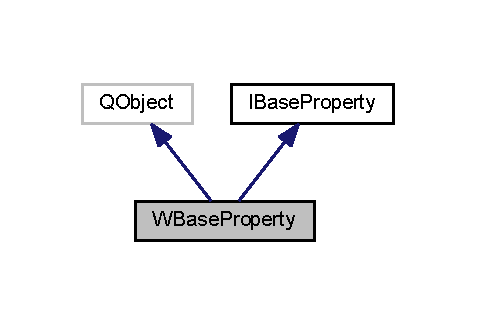
\includegraphics[width=229pt]{class_w_base_property__inherit__graph}
\end{center}
\end{figure}


Collaboration diagram for W\-Base\-Property\-:
\nopagebreak
\begin{figure}[H]
\begin{center}
\leavevmode
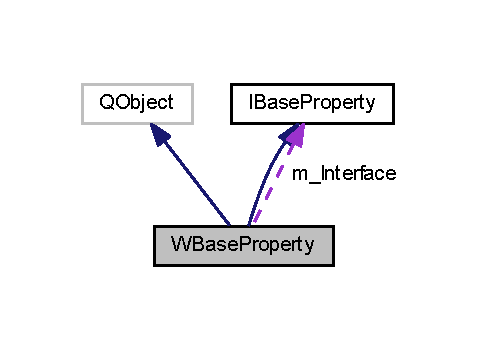
\includegraphics[width=231pt]{class_w_base_property__coll__graph}
\end{center}
\end{figure}
\subsection*{Public Slots}
\begin{DoxyCompactItemize}
\item 
void \hyperlink{class_w_base_property_a8f799b2109e340ce459c34d3fba5ad7a}{set\-Key} (Q\-String key)
\begin{DoxyCompactList}\small\item\em Sets the property key as a string. N\-O\-T\-E\-: Should be unique. \end{DoxyCompactList}\item 
void \hyperlink{class_w_base_property_a43fcf4605167b151729d051d37f3fd1d}{set\-Value\-Raw} (Q\-String value)
\begin{DoxyCompactList}\small\item\em Sets the property value as a raw string, ignoring the intended property format. \end{DoxyCompactList}\item 
void \hyperlink{class_w_base_property_ac3512628c101c5ba985eeae43d13521e}{set\-Comment} (Q\-String value)
\begin{DoxyCompactList}\small\item\em Sets the comment value as a raw string (without \char`\"{}//\char`\"{}). \end{DoxyCompactList}\end{DoxyCompactItemize}
\subsection*{Public Member Functions}
\begin{DoxyCompactItemize}
\item 
\hyperlink{class_w_base_property_a5f0a0f4e3f342d82ac9c9c45cb374c29}{W\-Base\-Property} (Q\-Object $\ast$parent=0)
\begin{DoxyCompactList}\small\item\em Constructor. Pass the \hyperlink{class_base_property}{Base\-Property} we are becoming a wrapper for. \end{DoxyCompactList}\item 
Q\-String \hyperlink{class_w_base_property_a4c0e55c7b0a19a7685b30a985b72524a}{get\-Key} () const 
\begin{DoxyCompactList}\small\item\em Returns the property key as a string. \end{DoxyCompactList}\item 
Q\-String \hyperlink{class_w_base_property_a49ba3186114cd7a0bb730a1a703af1eb}{get\-Value\-Raw} () const 
\begin{DoxyCompactList}\small\item\em Returns the property value as a raw string. \end{DoxyCompactList}\item 
Q\-String \hyperlink{class_w_base_property_a60750f9c78b6cbd7ec3fc1bfa9ae53fe}{get\-Comment} () const 
\begin{DoxyCompactList}\small\item\em Returns the comment value as a raw string (without \char`\"{}//\char`\"{}). \end{DoxyCompactList}\end{DoxyCompactItemize}
\subsection*{Protected Attributes}
\begin{DoxyCompactItemize}
\item 
\hyperlink{class_i_base_property}{I\-Base\-Property} $\ast$ \hyperlink{class_w_base_property_a8c25b5b13019cf65037147da7b03c643}{m\-\_\-\-Interface}
\end{DoxyCompactItemize}


\subsection{Detailed Description}
Base property interface wrapper. 

To avoid multiple Q\-Object inheritance errors, defining slots in interfaces requires the use of a wrapper object. To connect a signal to a slot on a \hyperlink{class_base_property}{Base\-Property} object, call \hyperlink{class_base_property_a032130dea4bd72ee8dd80dcfa7d5f37a}{Base\-Property\-::slots\-Base()} to return a pointer to this wrapper, then choose the desired slot. 

\subsection{Constructor \& Destructor Documentation}
\hypertarget{class_w_base_property_a5f0a0f4e3f342d82ac9c9c45cb374c29}{\index{W\-Base\-Property@{W\-Base\-Property}!W\-Base\-Property@{W\-Base\-Property}}
\index{W\-Base\-Property@{W\-Base\-Property}!WBaseProperty@{W\-Base\-Property}}
\subsubsection[{W\-Base\-Property}]{\setlength{\rightskip}{0pt plus 5cm}W\-Base\-Property\-::\-W\-Base\-Property (
\begin{DoxyParamCaption}
\item[{Q\-Object $\ast$}]{parent = {\ttfamily 0}}
\end{DoxyParamCaption}
)\hspace{0.3cm}{\ttfamily [inline]}}}\label{class_w_base_property_a5f0a0f4e3f342d82ac9c9c45cb374c29}


Constructor. Pass the \hyperlink{class_base_property}{Base\-Property} we are becoming a wrapper for. 


\begin{DoxyParams}{Parameters}
{\em parent} & \hyperlink{class_base_property}{Base\-Property} to wrap (object, not the interface). \\
\hline
\end{DoxyParams}


\subsection{Member Function Documentation}
\hypertarget{class_w_base_property_a60750f9c78b6cbd7ec3fc1bfa9ae53fe}{\index{W\-Base\-Property@{W\-Base\-Property}!get\-Comment@{get\-Comment}}
\index{get\-Comment@{get\-Comment}!WBaseProperty@{W\-Base\-Property}}
\subsubsection[{get\-Comment}]{\setlength{\rightskip}{0pt plus 5cm}Q\-String W\-Base\-Property\-::get\-Comment (
\begin{DoxyParamCaption}
{}
\end{DoxyParamCaption}
) const\hspace{0.3cm}{\ttfamily [inline]}, {\ttfamily [virtual]}}}\label{class_w_base_property_a60750f9c78b6cbd7ec3fc1bfa9ae53fe}


Returns the comment value as a raw string (without \char`\"{}//\char`\"{}). 

\begin{DoxyReturn}{Returns}
Unformatted comment string. 
\end{DoxyReturn}


Implements \hyperlink{class_i_base_property_a53f9fd81c8247dfce1ac651576dd4119}{I\-Base\-Property}.

\hypertarget{class_w_base_property_a4c0e55c7b0a19a7685b30a985b72524a}{\index{W\-Base\-Property@{W\-Base\-Property}!get\-Key@{get\-Key}}
\index{get\-Key@{get\-Key}!WBaseProperty@{W\-Base\-Property}}
\subsubsection[{get\-Key}]{\setlength{\rightskip}{0pt plus 5cm}Q\-String W\-Base\-Property\-::get\-Key (
\begin{DoxyParamCaption}
{}
\end{DoxyParamCaption}
) const\hspace{0.3cm}{\ttfamily [inline]}, {\ttfamily [virtual]}}}\label{class_w_base_property_a4c0e55c7b0a19a7685b30a985b72524a}


Returns the property key as a string. 

\begin{DoxyReturn}{Returns}
Q\-String representing the property's key. 
\end{DoxyReturn}


Implements \hyperlink{class_i_base_property_acbec936e956aa7fe59737af25e8b1962}{I\-Base\-Property}.

\hypertarget{class_w_base_property_a49ba3186114cd7a0bb730a1a703af1eb}{\index{W\-Base\-Property@{W\-Base\-Property}!get\-Value\-Raw@{get\-Value\-Raw}}
\index{get\-Value\-Raw@{get\-Value\-Raw}!WBaseProperty@{W\-Base\-Property}}
\subsubsection[{get\-Value\-Raw}]{\setlength{\rightskip}{0pt plus 5cm}Q\-String W\-Base\-Property\-::get\-Value\-Raw (
\begin{DoxyParamCaption}
{}
\end{DoxyParamCaption}
) const\hspace{0.3cm}{\ttfamily [inline]}, {\ttfamily [virtual]}}}\label{class_w_base_property_a49ba3186114cd7a0bb730a1a703af1eb}


Returns the property value as a raw string. 

\begin{DoxyReturn}{Returns}
Q\-String representation of the value the property holds. 
\end{DoxyReturn}


Implements \hyperlink{class_i_base_property_adf7edb55057975980bac6b6fc5514d15}{I\-Base\-Property}.

\hypertarget{class_w_base_property_ac3512628c101c5ba985eeae43d13521e}{\index{W\-Base\-Property@{W\-Base\-Property}!set\-Comment@{set\-Comment}}
\index{set\-Comment@{set\-Comment}!WBaseProperty@{W\-Base\-Property}}
\subsubsection[{set\-Comment}]{\setlength{\rightskip}{0pt plus 5cm}void W\-Base\-Property\-::set\-Comment (
\begin{DoxyParamCaption}
\item[{Q\-String}]{value}
\end{DoxyParamCaption}
)\hspace{0.3cm}{\ttfamily [inline]}, {\ttfamily [slot]}}}\label{class_w_base_property_ac3512628c101c5ba985eeae43d13521e}


Sets the comment value as a raw string (without \char`\"{}//\char`\"{}). 


\begin{DoxyParams}{Parameters}
{\em value} & Comment string to set. \\
\hline
\end{DoxyParams}
\hypertarget{class_w_base_property_a8f799b2109e340ce459c34d3fba5ad7a}{\index{W\-Base\-Property@{W\-Base\-Property}!set\-Key@{set\-Key}}
\index{set\-Key@{set\-Key}!WBaseProperty@{W\-Base\-Property}}
\subsubsection[{set\-Key}]{\setlength{\rightskip}{0pt plus 5cm}void W\-Base\-Property\-::set\-Key (
\begin{DoxyParamCaption}
\item[{Q\-String}]{key}
\end{DoxyParamCaption}
)\hspace{0.3cm}{\ttfamily [inline]}, {\ttfamily [slot]}}}\label{class_w_base_property_a8f799b2109e340ce459c34d3fba5ad7a}


Sets the property key as a string. N\-O\-T\-E\-: Should be unique. 


\begin{DoxyParams}{Parameters}
{\em key} & The key to set. \\
\hline
\end{DoxyParams}
\hypertarget{class_w_base_property_a43fcf4605167b151729d051d37f3fd1d}{\index{W\-Base\-Property@{W\-Base\-Property}!set\-Value\-Raw@{set\-Value\-Raw}}
\index{set\-Value\-Raw@{set\-Value\-Raw}!WBaseProperty@{W\-Base\-Property}}
\subsubsection[{set\-Value\-Raw}]{\setlength{\rightskip}{0pt plus 5cm}void W\-Base\-Property\-::set\-Value\-Raw (
\begin{DoxyParamCaption}
\item[{Q\-String}]{value}
\end{DoxyParamCaption}
)\hspace{0.3cm}{\ttfamily [inline]}, {\ttfamily [slot]}}}\label{class_w_base_property_a43fcf4605167b151729d051d37f3fd1d}


Sets the property value as a raw string, ignoring the intended property format. 


\begin{DoxyParams}{Parameters}
{\em value} & String value to set. \\
\hline
\end{DoxyParams}


\subsection{Member Data Documentation}
\hypertarget{class_w_base_property_a8c25b5b13019cf65037147da7b03c643}{\index{W\-Base\-Property@{W\-Base\-Property}!m\-\_\-\-Interface@{m\-\_\-\-Interface}}
\index{m\-\_\-\-Interface@{m\-\_\-\-Interface}!WBaseProperty@{W\-Base\-Property}}
\subsubsection[{m\-\_\-\-Interface}]{\setlength{\rightskip}{0pt plus 5cm}{\bf I\-Base\-Property}$\ast$ W\-Base\-Property\-::m\-\_\-\-Interface\hspace{0.3cm}{\ttfamily [protected]}}}\label{class_w_base_property_a8c25b5b13019cf65037147da7b03c643}
The interface whose functions we bind to. 

The documentation for this class was generated from the following file\-:\begin{DoxyCompactItemize}
\item 
app/\hyperlink{baseproperty_8h}{baseproperty.\-h}\end{DoxyCompactItemize}

\hypertarget{class_w_double_property}{\section{W\-Double\-Property Class Reference}
\label{class_w_double_property}\index{W\-Double\-Property@{W\-Double\-Property}}
}


M\-A\-C\-R\-O P\-R\-O\-P\-E\-R\-T\-Y I\-N\-T\-E\-R\-F\-A\-C\-E W\-R\-A\-P\-P\-E\-R F\-O\-R \hyperlink{class_i_double_property}{I\-Double\-Property} .  




{\ttfamily \#include $<$property.\-h$>$}



Inheritance diagram for W\-Double\-Property\-:
\nopagebreak
\begin{figure}[H]
\begin{center}
\leavevmode
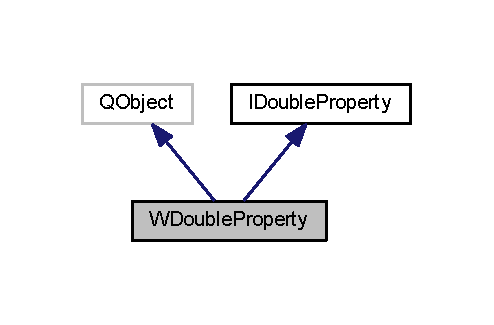
\includegraphics[width=237pt]{class_w_double_property__inherit__graph}
\end{center}
\end{figure}


Collaboration diagram for W\-Double\-Property\-:
\nopagebreak
\begin{figure}[H]
\begin{center}
\leavevmode
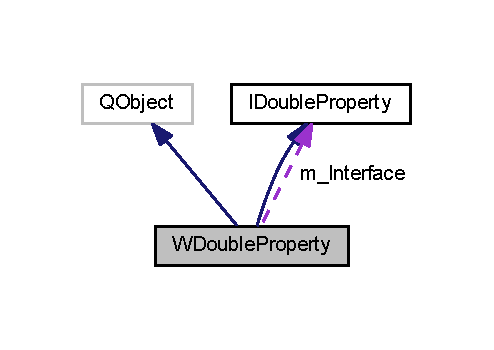
\includegraphics[width=237pt]{class_w_double_property__coll__graph}
\end{center}
\end{figure}
\subsection*{Public Slots}
\begin{DoxyCompactItemize}
\item 
void \hyperlink{class_w_double_property_a710f9b1c3c4a12682e9fa257b832ae89}{set\-Value} (double value)
\begin{DoxyCompactList}\small\item\em Sets the property's value as double . \end{DoxyCompactList}\item 
bool \hyperlink{class_w_double_property_a11a0a8b257e291fe896848a772e0505b}{pass\-To} (\hyperlink{class_property_variant}{Property\-Variant} $\ast$variant)
\begin{DoxyCompactList}\small\item\em Passes the property's value to the variant. \end{DoxyCompactList}\end{DoxyCompactItemize}
\subsection*{Public Member Functions}
\begin{DoxyCompactItemize}
\item 
\hyperlink{class_w_double_property_a7af52228cc8bbd608ef0df519f079533}{W\-Double\-Property} (Q\-Object $\ast$parent=0)
\begin{DoxyCompactList}\small\item\em Constructor. Pass the object which implements the interface as parent. \end{DoxyCompactList}\item 
double \hyperlink{class_w_double_property_ac771c45522b2682056081700effc7930}{get\-Value} (bool $\ast$success) const 
\begin{DoxyCompactList}\small\item\em Gets this property's value as double . \end{DoxyCompactList}\item 
bool \hyperlink{class_w_double_property_acf72db76ced6c2dc50027bc2714be73b}{can\-Convert} () const 
\begin{DoxyCompactList}\small\item\em Returns whether or not the property's value can be successfully converted. \end{DoxyCompactList}\end{DoxyCompactItemize}
\subsection*{Protected Attributes}
\begin{DoxyCompactItemize}
\item 
\hyperlink{class_i_double_property}{I\-Double\-Property} $\ast$ \hyperlink{class_w_double_property_aa40ee58413b2eb1431bcc98962e59c64}{m\-\_\-\-Interface}
\end{DoxyCompactItemize}


\subsection{Detailed Description}
M\-A\-C\-R\-O P\-R\-O\-P\-E\-R\-T\-Y I\-N\-T\-E\-R\-F\-A\-C\-E W\-R\-A\-P\-P\-E\-R F\-O\-R \hyperlink{class_i_double_property}{I\-Double\-Property} . 

Wrapper for the \hyperlink{class_i_double_property}{I\-Double\-Property} interface that facilitates binding of slots to the main class. 

\subsection{Constructor \& Destructor Documentation}
\hypertarget{class_w_double_property_a7af52228cc8bbd608ef0df519f079533}{\index{W\-Double\-Property@{W\-Double\-Property}!W\-Double\-Property@{W\-Double\-Property}}
\index{W\-Double\-Property@{W\-Double\-Property}!WDoubleProperty@{W\-Double\-Property}}
\subsubsection[{W\-Double\-Property}]{\setlength{\rightskip}{0pt plus 5cm}W\-Double\-Property\-::\-W\-Double\-Property (
\begin{DoxyParamCaption}
\item[{Q\-Object $\ast$}]{parent = {\ttfamily 0}}
\end{DoxyParamCaption}
)\hspace{0.3cm}{\ttfamily [inline]}}}\label{class_w_double_property_a7af52228cc8bbd608ef0df519f079533}


Constructor. Pass the object which implements the interface as parent. 


\begin{DoxyParams}{Parameters}
{\em parent} & Object who implements \hyperlink{class_i_double_property}{I\-Double\-Property} and whose functions this wrapper should bind slots to. \\
\hline
\end{DoxyParams}


\subsection{Member Function Documentation}
\hypertarget{class_w_double_property_acf72db76ced6c2dc50027bc2714be73b}{\index{W\-Double\-Property@{W\-Double\-Property}!can\-Convert@{can\-Convert}}
\index{can\-Convert@{can\-Convert}!WDoubleProperty@{W\-Double\-Property}}
\subsubsection[{can\-Convert}]{\setlength{\rightskip}{0pt plus 5cm}bool W\-Double\-Property\-::can\-Convert (
\begin{DoxyParamCaption}
{}
\end{DoxyParamCaption}
) const\hspace{0.3cm}{\ttfamily [inline]}, {\ttfamily [virtual]}}}\label{class_w_double_property_acf72db76ced6c2dc50027bc2714be73b}


Returns whether or not the property's value can be successfully converted. 

\begin{DoxyReturn}{Returns}
True if conversion is possible, false otherwise. 
\end{DoxyReturn}


Implements \hyperlink{class_i_double_property_afe5368913e955ec08c2797521d43d24a}{I\-Double\-Property}.

\hypertarget{class_w_double_property_ac771c45522b2682056081700effc7930}{\index{W\-Double\-Property@{W\-Double\-Property}!get\-Value@{get\-Value}}
\index{get\-Value@{get\-Value}!WDoubleProperty@{W\-Double\-Property}}
\subsubsection[{get\-Value}]{\setlength{\rightskip}{0pt plus 5cm}double W\-Double\-Property\-::get\-Value (
\begin{DoxyParamCaption}
\item[{bool $\ast$}]{success}
\end{DoxyParamCaption}
) const\hspace{0.3cm}{\ttfamily [inline]}, {\ttfamily [virtual]}}}\label{class_w_double_property_ac771c45522b2682056081700effc7930}


Gets this property's value as double . 


\begin{DoxyParams}{Parameters}
{\em success} & True if conversion was successful, false otherwise.\\
\hline
\end{DoxyParams}
\begin{DoxyReturn}{Returns}
The property's value. 
\end{DoxyReturn}


Implements \hyperlink{class_i_double_property_af9143d685793a22249eb50b2515260ac}{I\-Double\-Property}.

\hypertarget{class_w_double_property_a11a0a8b257e291fe896848a772e0505b}{\index{W\-Double\-Property@{W\-Double\-Property}!pass\-To@{pass\-To}}
\index{pass\-To@{pass\-To}!WDoubleProperty@{W\-Double\-Property}}
\subsubsection[{pass\-To}]{\setlength{\rightskip}{0pt plus 5cm}bool W\-Double\-Property\-::pass\-To (
\begin{DoxyParamCaption}
\item[{{\bf Property\-Variant} $\ast$}]{variant}
\end{DoxyParamCaption}
)\hspace{0.3cm}{\ttfamily [inline]}, {\ttfamily [slot]}}}\label{class_w_double_property_a11a0a8b257e291fe896848a772e0505b}


Passes the property's value to the variant. 


\begin{DoxyParams}{Parameters}
{\em variant} & Variant to pass to.\\
\hline
\end{DoxyParams}
\begin{DoxyReturn}{Returns}
True if conversion succeeded, false otherwise. 
\end{DoxyReturn}
\hypertarget{class_w_double_property_a710f9b1c3c4a12682e9fa257b832ae89}{\index{W\-Double\-Property@{W\-Double\-Property}!set\-Value@{set\-Value}}
\index{set\-Value@{set\-Value}!WDoubleProperty@{W\-Double\-Property}}
\subsubsection[{set\-Value}]{\setlength{\rightskip}{0pt plus 5cm}void W\-Double\-Property\-::set\-Value (
\begin{DoxyParamCaption}
\item[{double}]{value}
\end{DoxyParamCaption}
)\hspace{0.3cm}{\ttfamily [inline]}, {\ttfamily [slot]}}}\label{class_w_double_property_a710f9b1c3c4a12682e9fa257b832ae89}


Sets the property's value as double . 


\begin{DoxyParams}{Parameters}
{\em value} & Value to set. \\
\hline
\end{DoxyParams}


\subsection{Member Data Documentation}
\hypertarget{class_w_double_property_aa40ee58413b2eb1431bcc98962e59c64}{\index{W\-Double\-Property@{W\-Double\-Property}!m\-\_\-\-Interface@{m\-\_\-\-Interface}}
\index{m\-\_\-\-Interface@{m\-\_\-\-Interface}!WDoubleProperty@{W\-Double\-Property}}
\subsubsection[{m\-\_\-\-Interface}]{\setlength{\rightskip}{0pt plus 5cm}{\bf I\-Double\-Property}$\ast$ W\-Double\-Property\-::m\-\_\-\-Interface\hspace{0.3cm}{\ttfamily [protected]}}}\label{class_w_double_property_aa40ee58413b2eb1431bcc98962e59c64}
The interface that represents the bound functions on the parent object. 

The documentation for this class was generated from the following file\-:\begin{DoxyCompactItemize}
\item 
app/\hyperlink{property_8h}{property.\-h}\end{DoxyCompactItemize}

\hypertarget{class_w_float_property}{\section{W\-Float\-Property Class Reference}
\label{class_w_float_property}\index{W\-Float\-Property@{W\-Float\-Property}}
}


M\-A\-C\-R\-O P\-R\-O\-P\-E\-R\-T\-Y I\-N\-T\-E\-R\-F\-A\-C\-E W\-R\-A\-P\-P\-E\-R F\-O\-R \hyperlink{class_i_float_property}{I\-Float\-Property} .  




{\ttfamily \#include $<$property.\-h$>$}



Inheritance diagram for W\-Float\-Property\-:
\nopagebreak
\begin{figure}[H]
\begin{center}
\leavevmode
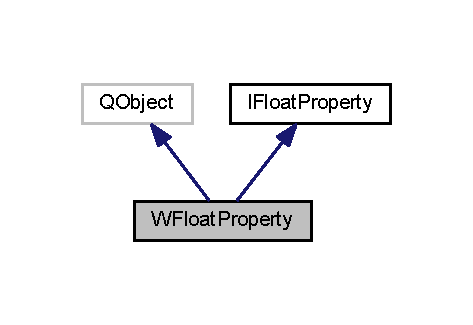
\includegraphics[width=227pt]{class_w_float_property__inherit__graph}
\end{center}
\end{figure}


Collaboration diagram for W\-Float\-Property\-:
\nopagebreak
\begin{figure}[H]
\begin{center}
\leavevmode
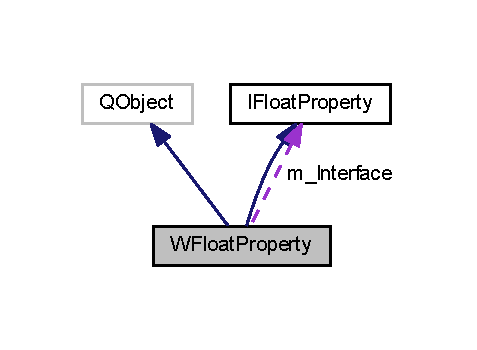
\includegraphics[width=229pt]{class_w_float_property__coll__graph}
\end{center}
\end{figure}
\subsection*{Public Slots}
\begin{DoxyCompactItemize}
\item 
void \hyperlink{class_w_float_property_addd5ab4fe5a6b75f12e604c994c4d096}{set\-Value} (float value)
\begin{DoxyCompactList}\small\item\em Sets the property's value as float . \end{DoxyCompactList}\item 
bool \hyperlink{class_w_float_property_a6da253f88b37ee72187107956200a2ba}{pass\-To} (\hyperlink{class_property_variant}{Property\-Variant} $\ast$variant)
\begin{DoxyCompactList}\small\item\em Passes the property's value to the variant. \end{DoxyCompactList}\end{DoxyCompactItemize}
\subsection*{Public Member Functions}
\begin{DoxyCompactItemize}
\item 
\hyperlink{class_w_float_property_a0feb213835bd18827d230c8de6c8b788}{W\-Float\-Property} (Q\-Object $\ast$parent=0)
\begin{DoxyCompactList}\small\item\em Constructor. Pass the object which implements the interface as parent. \end{DoxyCompactList}\item 
float \hyperlink{class_w_float_property_acdfaccfb44bff32042d5eecb377f406d}{get\-Value} (bool $\ast$success) const 
\begin{DoxyCompactList}\small\item\em Gets this property's value as float . \end{DoxyCompactList}\item 
bool \hyperlink{class_w_float_property_a7eee2964a782c7909b11f7621504fc11}{can\-Convert} () const 
\begin{DoxyCompactList}\small\item\em Returns whether or not the property's value can be successfully converted. \end{DoxyCompactList}\end{DoxyCompactItemize}
\subsection*{Protected Attributes}
\begin{DoxyCompactItemize}
\item 
\hyperlink{class_i_float_property}{I\-Float\-Property} $\ast$ \hyperlink{class_w_float_property_aee5767ac1ab391a1da6f396ed334e98b}{m\-\_\-\-Interface}
\end{DoxyCompactItemize}


\subsection{Detailed Description}
M\-A\-C\-R\-O P\-R\-O\-P\-E\-R\-T\-Y I\-N\-T\-E\-R\-F\-A\-C\-E W\-R\-A\-P\-P\-E\-R F\-O\-R \hyperlink{class_i_float_property}{I\-Float\-Property} . 

Wrapper for the \hyperlink{class_i_float_property}{I\-Float\-Property} interface that facilitates binding of slots to the main class. 

\subsection{Constructor \& Destructor Documentation}
\hypertarget{class_w_float_property_a0feb213835bd18827d230c8de6c8b788}{\index{W\-Float\-Property@{W\-Float\-Property}!W\-Float\-Property@{W\-Float\-Property}}
\index{W\-Float\-Property@{W\-Float\-Property}!WFloatProperty@{W\-Float\-Property}}
\subsubsection[{W\-Float\-Property}]{\setlength{\rightskip}{0pt plus 5cm}W\-Float\-Property\-::\-W\-Float\-Property (
\begin{DoxyParamCaption}
\item[{Q\-Object $\ast$}]{parent = {\ttfamily 0}}
\end{DoxyParamCaption}
)\hspace{0.3cm}{\ttfamily [inline]}}}\label{class_w_float_property_a0feb213835bd18827d230c8de6c8b788}


Constructor. Pass the object which implements the interface as parent. 


\begin{DoxyParams}{Parameters}
{\em parent} & Object who implements \hyperlink{class_i_float_property}{I\-Float\-Property} and whose functions this wrapper should bind slots to. \\
\hline
\end{DoxyParams}


\subsection{Member Function Documentation}
\hypertarget{class_w_float_property_a7eee2964a782c7909b11f7621504fc11}{\index{W\-Float\-Property@{W\-Float\-Property}!can\-Convert@{can\-Convert}}
\index{can\-Convert@{can\-Convert}!WFloatProperty@{W\-Float\-Property}}
\subsubsection[{can\-Convert}]{\setlength{\rightskip}{0pt plus 5cm}bool W\-Float\-Property\-::can\-Convert (
\begin{DoxyParamCaption}
{}
\end{DoxyParamCaption}
) const\hspace{0.3cm}{\ttfamily [inline]}, {\ttfamily [virtual]}}}\label{class_w_float_property_a7eee2964a782c7909b11f7621504fc11}


Returns whether or not the property's value can be successfully converted. 

\begin{DoxyReturn}{Returns}
True if conversion is possible, false otherwise. 
\end{DoxyReturn}


Implements \hyperlink{class_i_float_property_a1e460fc2f90845794910bc74aabe5236}{I\-Float\-Property}.

\hypertarget{class_w_float_property_acdfaccfb44bff32042d5eecb377f406d}{\index{W\-Float\-Property@{W\-Float\-Property}!get\-Value@{get\-Value}}
\index{get\-Value@{get\-Value}!WFloatProperty@{W\-Float\-Property}}
\subsubsection[{get\-Value}]{\setlength{\rightskip}{0pt plus 5cm}float W\-Float\-Property\-::get\-Value (
\begin{DoxyParamCaption}
\item[{bool $\ast$}]{success}
\end{DoxyParamCaption}
) const\hspace{0.3cm}{\ttfamily [inline]}, {\ttfamily [virtual]}}}\label{class_w_float_property_acdfaccfb44bff32042d5eecb377f406d}


Gets this property's value as float . 


\begin{DoxyParams}{Parameters}
{\em success} & True if conversion was successful, false otherwise.\\
\hline
\end{DoxyParams}
\begin{DoxyReturn}{Returns}
The property's value. 
\end{DoxyReturn}


Implements \hyperlink{class_i_float_property_a5f3b98066c898de66db9141b01253d60}{I\-Float\-Property}.

\hypertarget{class_w_float_property_a6da253f88b37ee72187107956200a2ba}{\index{W\-Float\-Property@{W\-Float\-Property}!pass\-To@{pass\-To}}
\index{pass\-To@{pass\-To}!WFloatProperty@{W\-Float\-Property}}
\subsubsection[{pass\-To}]{\setlength{\rightskip}{0pt plus 5cm}bool W\-Float\-Property\-::pass\-To (
\begin{DoxyParamCaption}
\item[{{\bf Property\-Variant} $\ast$}]{variant}
\end{DoxyParamCaption}
)\hspace{0.3cm}{\ttfamily [inline]}, {\ttfamily [slot]}}}\label{class_w_float_property_a6da253f88b37ee72187107956200a2ba}


Passes the property's value to the variant. 


\begin{DoxyParams}{Parameters}
{\em variant} & Variant to pass to.\\
\hline
\end{DoxyParams}
\begin{DoxyReturn}{Returns}
True if conversion succeeded, false otherwise. 
\end{DoxyReturn}
\hypertarget{class_w_float_property_addd5ab4fe5a6b75f12e604c994c4d096}{\index{W\-Float\-Property@{W\-Float\-Property}!set\-Value@{set\-Value}}
\index{set\-Value@{set\-Value}!WFloatProperty@{W\-Float\-Property}}
\subsubsection[{set\-Value}]{\setlength{\rightskip}{0pt plus 5cm}void W\-Float\-Property\-::set\-Value (
\begin{DoxyParamCaption}
\item[{float}]{value}
\end{DoxyParamCaption}
)\hspace{0.3cm}{\ttfamily [inline]}, {\ttfamily [slot]}}}\label{class_w_float_property_addd5ab4fe5a6b75f12e604c994c4d096}


Sets the property's value as float . 


\begin{DoxyParams}{Parameters}
{\em value} & Value to set. \\
\hline
\end{DoxyParams}


\subsection{Member Data Documentation}
\hypertarget{class_w_float_property_aee5767ac1ab391a1da6f396ed334e98b}{\index{W\-Float\-Property@{W\-Float\-Property}!m\-\_\-\-Interface@{m\-\_\-\-Interface}}
\index{m\-\_\-\-Interface@{m\-\_\-\-Interface}!WFloatProperty@{W\-Float\-Property}}
\subsubsection[{m\-\_\-\-Interface}]{\setlength{\rightskip}{0pt plus 5cm}{\bf I\-Float\-Property}$\ast$ W\-Float\-Property\-::m\-\_\-\-Interface\hspace{0.3cm}{\ttfamily [protected]}}}\label{class_w_float_property_aee5767ac1ab391a1da6f396ed334e98b}
The interface that represents the bound functions on the parent object. 

The documentation for this class was generated from the following file\-:\begin{DoxyCompactItemize}
\item 
app/\hyperlink{property_8h}{property.\-h}\end{DoxyCompactItemize}

\hypertarget{class_w_int_property}{\section{W\-Int\-Property Class Reference}
\label{class_w_int_property}\index{W\-Int\-Property@{W\-Int\-Property}}
}


M\-A\-C\-R\-O P\-R\-O\-P\-E\-R\-T\-Y I\-N\-T\-E\-R\-F\-A\-C\-E W\-R\-A\-P\-P\-E\-R F\-O\-R \hyperlink{class_i_int_property}{I\-Int\-Property} .  




{\ttfamily \#include $<$property.\-h$>$}



Inheritance diagram for W\-Int\-Property\-:
\nopagebreak
\begin{figure}[H]
\begin{center}
\leavevmode
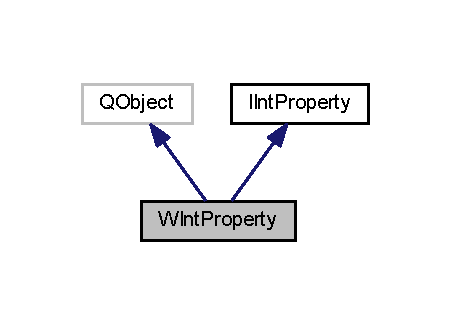
\includegraphics[width=217pt]{class_w_int_property__inherit__graph}
\end{center}
\end{figure}


Collaboration diagram for W\-Int\-Property\-:
\nopagebreak
\begin{figure}[H]
\begin{center}
\leavevmode
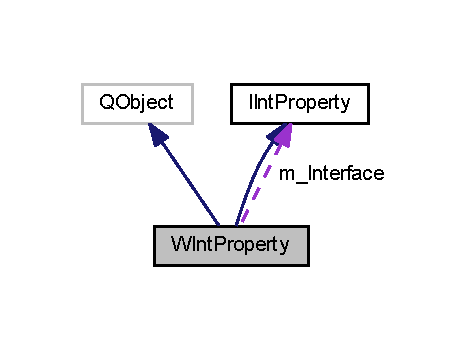
\includegraphics[width=225pt]{class_w_int_property__coll__graph}
\end{center}
\end{figure}
\subsection*{Public Slots}
\begin{DoxyCompactItemize}
\item 
void \hyperlink{class_w_int_property_a799b26a1c6622fd70068deed73547f6a}{set\-Value} (int value)
\begin{DoxyCompactList}\small\item\em Sets the property's value as int . \end{DoxyCompactList}\item 
bool \hyperlink{class_w_int_property_a92a1f77aac38b9660537122ed55c5e0b}{pass\-To} (\hyperlink{class_property_variant}{Property\-Variant} $\ast$variant)
\begin{DoxyCompactList}\small\item\em Passes the property's value to the variant. \end{DoxyCompactList}\end{DoxyCompactItemize}
\subsection*{Public Member Functions}
\begin{DoxyCompactItemize}
\item 
\hyperlink{class_w_int_property_a5d3ce207add6e3a5f3868010cf9f37e1}{W\-Int\-Property} (Q\-Object $\ast$parent=0)
\begin{DoxyCompactList}\small\item\em Constructor. Pass the object which implements the interface as parent. \end{DoxyCompactList}\item 
int \hyperlink{class_w_int_property_aea678a96a398024ac3cdcdb31e5999de}{get\-Value} (bool $\ast$success) const 
\begin{DoxyCompactList}\small\item\em Gets this property's value as int . \end{DoxyCompactList}\item 
bool \hyperlink{class_w_int_property_a2aadf339189421871abccd98b553ce6b}{can\-Convert} () const 
\begin{DoxyCompactList}\small\item\em Returns whether or not the property's value can be successfully converted. \end{DoxyCompactList}\end{DoxyCompactItemize}
\subsection*{Protected Attributes}
\begin{DoxyCompactItemize}
\item 
\hyperlink{class_i_int_property}{I\-Int\-Property} $\ast$ \hyperlink{class_w_int_property_a7c4faa1f37d022fe9bc1bd2da01c2213}{m\-\_\-\-Interface}
\end{DoxyCompactItemize}


\subsection{Detailed Description}
M\-A\-C\-R\-O P\-R\-O\-P\-E\-R\-T\-Y I\-N\-T\-E\-R\-F\-A\-C\-E W\-R\-A\-P\-P\-E\-R F\-O\-R \hyperlink{class_i_int_property}{I\-Int\-Property} . 

Wrapper for the \hyperlink{class_i_int_property}{I\-Int\-Property} interface that facilitates binding of slots to the main class. 

\subsection{Constructor \& Destructor Documentation}
\hypertarget{class_w_int_property_a5d3ce207add6e3a5f3868010cf9f37e1}{\index{W\-Int\-Property@{W\-Int\-Property}!W\-Int\-Property@{W\-Int\-Property}}
\index{W\-Int\-Property@{W\-Int\-Property}!WIntProperty@{W\-Int\-Property}}
\subsubsection[{W\-Int\-Property}]{\setlength{\rightskip}{0pt plus 5cm}W\-Int\-Property\-::\-W\-Int\-Property (
\begin{DoxyParamCaption}
\item[{Q\-Object $\ast$}]{parent = {\ttfamily 0}}
\end{DoxyParamCaption}
)\hspace{0.3cm}{\ttfamily [inline]}}}\label{class_w_int_property_a5d3ce207add6e3a5f3868010cf9f37e1}


Constructor. Pass the object which implements the interface as parent. 


\begin{DoxyParams}{Parameters}
{\em parent} & Object who implements \hyperlink{class_i_int_property}{I\-Int\-Property} and whose functions this wrapper should bind slots to. \\
\hline
\end{DoxyParams}


\subsection{Member Function Documentation}
\hypertarget{class_w_int_property_a2aadf339189421871abccd98b553ce6b}{\index{W\-Int\-Property@{W\-Int\-Property}!can\-Convert@{can\-Convert}}
\index{can\-Convert@{can\-Convert}!WIntProperty@{W\-Int\-Property}}
\subsubsection[{can\-Convert}]{\setlength{\rightskip}{0pt plus 5cm}bool W\-Int\-Property\-::can\-Convert (
\begin{DoxyParamCaption}
{}
\end{DoxyParamCaption}
) const\hspace{0.3cm}{\ttfamily [inline]}, {\ttfamily [virtual]}}}\label{class_w_int_property_a2aadf339189421871abccd98b553ce6b}


Returns whether or not the property's value can be successfully converted. 

\begin{DoxyReturn}{Returns}
True if conversion is possible, false otherwise. 
\end{DoxyReturn}


Implements \hyperlink{class_i_int_property_a25375f7c817ab7a1aeaef72a5bcfafdd}{I\-Int\-Property}.

\hypertarget{class_w_int_property_aea678a96a398024ac3cdcdb31e5999de}{\index{W\-Int\-Property@{W\-Int\-Property}!get\-Value@{get\-Value}}
\index{get\-Value@{get\-Value}!WIntProperty@{W\-Int\-Property}}
\subsubsection[{get\-Value}]{\setlength{\rightskip}{0pt plus 5cm}int W\-Int\-Property\-::get\-Value (
\begin{DoxyParamCaption}
\item[{bool $\ast$}]{success}
\end{DoxyParamCaption}
) const\hspace{0.3cm}{\ttfamily [inline]}, {\ttfamily [virtual]}}}\label{class_w_int_property_aea678a96a398024ac3cdcdb31e5999de}


Gets this property's value as int . 


\begin{DoxyParams}{Parameters}
{\em success} & True if conversion was successful, false otherwise.\\
\hline
\end{DoxyParams}
\begin{DoxyReturn}{Returns}
The property's value. 
\end{DoxyReturn}


Implements \hyperlink{class_i_int_property_a32bd5be46bee5c4a53180498767f51d0}{I\-Int\-Property}.

\hypertarget{class_w_int_property_a92a1f77aac38b9660537122ed55c5e0b}{\index{W\-Int\-Property@{W\-Int\-Property}!pass\-To@{pass\-To}}
\index{pass\-To@{pass\-To}!WIntProperty@{W\-Int\-Property}}
\subsubsection[{pass\-To}]{\setlength{\rightskip}{0pt plus 5cm}bool W\-Int\-Property\-::pass\-To (
\begin{DoxyParamCaption}
\item[{{\bf Property\-Variant} $\ast$}]{variant}
\end{DoxyParamCaption}
)\hspace{0.3cm}{\ttfamily [inline]}, {\ttfamily [slot]}}}\label{class_w_int_property_a92a1f77aac38b9660537122ed55c5e0b}


Passes the property's value to the variant. 


\begin{DoxyParams}{Parameters}
{\em variant} & Variant to pass to.\\
\hline
\end{DoxyParams}
\begin{DoxyReturn}{Returns}
True if conversion succeeded, false otherwise. 
\end{DoxyReturn}
\hypertarget{class_w_int_property_a799b26a1c6622fd70068deed73547f6a}{\index{W\-Int\-Property@{W\-Int\-Property}!set\-Value@{set\-Value}}
\index{set\-Value@{set\-Value}!WIntProperty@{W\-Int\-Property}}
\subsubsection[{set\-Value}]{\setlength{\rightskip}{0pt plus 5cm}void W\-Int\-Property\-::set\-Value (
\begin{DoxyParamCaption}
\item[{int}]{value}
\end{DoxyParamCaption}
)\hspace{0.3cm}{\ttfamily [inline]}, {\ttfamily [slot]}}}\label{class_w_int_property_a799b26a1c6622fd70068deed73547f6a}


Sets the property's value as int . 


\begin{DoxyParams}{Parameters}
{\em value} & Value to set. \\
\hline
\end{DoxyParams}


\subsection{Member Data Documentation}
\hypertarget{class_w_int_property_a7c4faa1f37d022fe9bc1bd2da01c2213}{\index{W\-Int\-Property@{W\-Int\-Property}!m\-\_\-\-Interface@{m\-\_\-\-Interface}}
\index{m\-\_\-\-Interface@{m\-\_\-\-Interface}!WIntProperty@{W\-Int\-Property}}
\subsubsection[{m\-\_\-\-Interface}]{\setlength{\rightskip}{0pt plus 5cm}{\bf I\-Int\-Property}$\ast$ W\-Int\-Property\-::m\-\_\-\-Interface\hspace{0.3cm}{\ttfamily [protected]}}}\label{class_w_int_property_a7c4faa1f37d022fe9bc1bd2da01c2213}
The interface that represents the bound functions on the parent object. 

The documentation for this class was generated from the following file\-:\begin{DoxyCompactItemize}
\item 
app/\hyperlink{property_8h}{property.\-h}\end{DoxyCompactItemize}

\hypertarget{class_w_long_long_property}{\section{W\-Long\-Long\-Property Class Reference}
\label{class_w_long_long_property}\index{W\-Long\-Long\-Property@{W\-Long\-Long\-Property}}
}


M\-A\-C\-R\-O P\-R\-O\-P\-E\-R\-T\-Y I\-N\-T\-E\-R\-F\-A\-C\-E W\-R\-A\-P\-P\-E\-R F\-O\-R \hyperlink{class_i_long_long_property}{I\-Long\-Long\-Property} .  




{\ttfamily \#include $<$property.\-h$>$}



Inheritance diagram for W\-Long\-Long\-Property\-:
\nopagebreak
\begin{figure}[H]
\begin{center}
\leavevmode
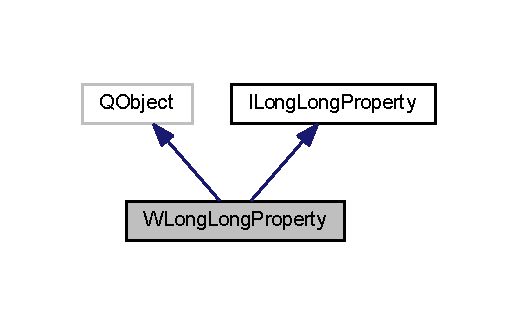
\includegraphics[width=249pt]{class_w_long_long_property__inherit__graph}
\end{center}
\end{figure}


Collaboration diagram for W\-Long\-Long\-Property\-:
\nopagebreak
\begin{figure}[H]
\begin{center}
\leavevmode
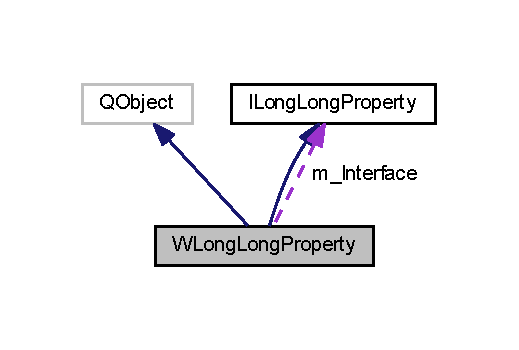
\includegraphics[width=249pt]{class_w_long_long_property__coll__graph}
\end{center}
\end{figure}
\subsection*{Public Slots}
\begin{DoxyCompactItemize}
\item 
void \hyperlink{class_w_long_long_property_aef758f4156c156c6a4750f81fd673f65}{set\-Value} (qlonglong value)
\begin{DoxyCompactList}\small\item\em Sets the property's value as qlonglong . \end{DoxyCompactList}\item 
bool \hyperlink{class_w_long_long_property_aae25a17ef3af73f647799dbc08be3dcd}{pass\-To} (\hyperlink{class_property_variant}{Property\-Variant} $\ast$variant)
\begin{DoxyCompactList}\small\item\em Passes the property's value to the variant. \end{DoxyCompactList}\end{DoxyCompactItemize}
\subsection*{Public Member Functions}
\begin{DoxyCompactItemize}
\item 
\hyperlink{class_w_long_long_property_a9005bf9802f0368cacd6d81e77abb514}{W\-Long\-Long\-Property} (Q\-Object $\ast$parent=0)
\begin{DoxyCompactList}\small\item\em Constructor. Pass the object which implements the interface as parent. \end{DoxyCompactList}\item 
qlonglong \hyperlink{class_w_long_long_property_abae79b01d411ec7f44aa2d93289ad63f}{get\-Value} (bool $\ast$success) const 
\begin{DoxyCompactList}\small\item\em Gets this property's value as qlonglong . \end{DoxyCompactList}\item 
bool \hyperlink{class_w_long_long_property_a5b553e3d82d48cb661ef6180fa8ed76e}{can\-Convert} () const 
\begin{DoxyCompactList}\small\item\em Returns whether or not the property's value can be successfully converted. \end{DoxyCompactList}\end{DoxyCompactItemize}
\subsection*{Protected Attributes}
\begin{DoxyCompactItemize}
\item 
\hyperlink{class_i_long_long_property}{I\-Long\-Long\-Property} $\ast$ \hyperlink{class_w_long_long_property_ae6b2b015e81593744f2ef962aa7c04b6}{m\-\_\-\-Interface}
\end{DoxyCompactItemize}


\subsection{Detailed Description}
M\-A\-C\-R\-O P\-R\-O\-P\-E\-R\-T\-Y I\-N\-T\-E\-R\-F\-A\-C\-E W\-R\-A\-P\-P\-E\-R F\-O\-R \hyperlink{class_i_long_long_property}{I\-Long\-Long\-Property} . 

Wrapper for the \hyperlink{class_i_long_long_property}{I\-Long\-Long\-Property} interface that facilitates binding of slots to the main class. 

\subsection{Constructor \& Destructor Documentation}
\hypertarget{class_w_long_long_property_a9005bf9802f0368cacd6d81e77abb514}{\index{W\-Long\-Long\-Property@{W\-Long\-Long\-Property}!W\-Long\-Long\-Property@{W\-Long\-Long\-Property}}
\index{W\-Long\-Long\-Property@{W\-Long\-Long\-Property}!WLongLongProperty@{W\-Long\-Long\-Property}}
\subsubsection[{W\-Long\-Long\-Property}]{\setlength{\rightskip}{0pt plus 5cm}W\-Long\-Long\-Property\-::\-W\-Long\-Long\-Property (
\begin{DoxyParamCaption}
\item[{Q\-Object $\ast$}]{parent = {\ttfamily 0}}
\end{DoxyParamCaption}
)\hspace{0.3cm}{\ttfamily [inline]}}}\label{class_w_long_long_property_a9005bf9802f0368cacd6d81e77abb514}


Constructor. Pass the object which implements the interface as parent. 


\begin{DoxyParams}{Parameters}
{\em parent} & Object who implements \hyperlink{class_i_long_long_property}{I\-Long\-Long\-Property} and whose functions this wrapper should bind slots to. \\
\hline
\end{DoxyParams}


\subsection{Member Function Documentation}
\hypertarget{class_w_long_long_property_a5b553e3d82d48cb661ef6180fa8ed76e}{\index{W\-Long\-Long\-Property@{W\-Long\-Long\-Property}!can\-Convert@{can\-Convert}}
\index{can\-Convert@{can\-Convert}!WLongLongProperty@{W\-Long\-Long\-Property}}
\subsubsection[{can\-Convert}]{\setlength{\rightskip}{0pt plus 5cm}bool W\-Long\-Long\-Property\-::can\-Convert (
\begin{DoxyParamCaption}
{}
\end{DoxyParamCaption}
) const\hspace{0.3cm}{\ttfamily [inline]}, {\ttfamily [virtual]}}}\label{class_w_long_long_property_a5b553e3d82d48cb661ef6180fa8ed76e}


Returns whether or not the property's value can be successfully converted. 

\begin{DoxyReturn}{Returns}
True if conversion is possible, false otherwise. 
\end{DoxyReturn}


Implements \hyperlink{class_i_long_long_property_a878b7753e3c53e966f9be8a3bd1e9b38}{I\-Long\-Long\-Property}.

\hypertarget{class_w_long_long_property_abae79b01d411ec7f44aa2d93289ad63f}{\index{W\-Long\-Long\-Property@{W\-Long\-Long\-Property}!get\-Value@{get\-Value}}
\index{get\-Value@{get\-Value}!WLongLongProperty@{W\-Long\-Long\-Property}}
\subsubsection[{get\-Value}]{\setlength{\rightskip}{0pt plus 5cm}qlonglong W\-Long\-Long\-Property\-::get\-Value (
\begin{DoxyParamCaption}
\item[{bool $\ast$}]{success}
\end{DoxyParamCaption}
) const\hspace{0.3cm}{\ttfamily [inline]}, {\ttfamily [virtual]}}}\label{class_w_long_long_property_abae79b01d411ec7f44aa2d93289ad63f}


Gets this property's value as qlonglong . 


\begin{DoxyParams}{Parameters}
{\em success} & True if conversion was successful, false otherwise.\\
\hline
\end{DoxyParams}
\begin{DoxyReturn}{Returns}
The property's value. 
\end{DoxyReturn}


Implements \hyperlink{class_i_long_long_property_a4364152258a2b085fa660ae34d106fdf}{I\-Long\-Long\-Property}.

\hypertarget{class_w_long_long_property_aae25a17ef3af73f647799dbc08be3dcd}{\index{W\-Long\-Long\-Property@{W\-Long\-Long\-Property}!pass\-To@{pass\-To}}
\index{pass\-To@{pass\-To}!WLongLongProperty@{W\-Long\-Long\-Property}}
\subsubsection[{pass\-To}]{\setlength{\rightskip}{0pt plus 5cm}bool W\-Long\-Long\-Property\-::pass\-To (
\begin{DoxyParamCaption}
\item[{{\bf Property\-Variant} $\ast$}]{variant}
\end{DoxyParamCaption}
)\hspace{0.3cm}{\ttfamily [inline]}, {\ttfamily [slot]}}}\label{class_w_long_long_property_aae25a17ef3af73f647799dbc08be3dcd}


Passes the property's value to the variant. 


\begin{DoxyParams}{Parameters}
{\em variant} & Variant to pass to.\\
\hline
\end{DoxyParams}
\begin{DoxyReturn}{Returns}
True if conversion succeeded, false otherwise. 
\end{DoxyReturn}
\hypertarget{class_w_long_long_property_aef758f4156c156c6a4750f81fd673f65}{\index{W\-Long\-Long\-Property@{W\-Long\-Long\-Property}!set\-Value@{set\-Value}}
\index{set\-Value@{set\-Value}!WLongLongProperty@{W\-Long\-Long\-Property}}
\subsubsection[{set\-Value}]{\setlength{\rightskip}{0pt plus 5cm}void W\-Long\-Long\-Property\-::set\-Value (
\begin{DoxyParamCaption}
\item[{qlonglong}]{value}
\end{DoxyParamCaption}
)\hspace{0.3cm}{\ttfamily [inline]}, {\ttfamily [slot]}}}\label{class_w_long_long_property_aef758f4156c156c6a4750f81fd673f65}


Sets the property's value as qlonglong . 


\begin{DoxyParams}{Parameters}
{\em value} & Value to set. \\
\hline
\end{DoxyParams}


\subsection{Member Data Documentation}
\hypertarget{class_w_long_long_property_ae6b2b015e81593744f2ef962aa7c04b6}{\index{W\-Long\-Long\-Property@{W\-Long\-Long\-Property}!m\-\_\-\-Interface@{m\-\_\-\-Interface}}
\index{m\-\_\-\-Interface@{m\-\_\-\-Interface}!WLongLongProperty@{W\-Long\-Long\-Property}}
\subsubsection[{m\-\_\-\-Interface}]{\setlength{\rightskip}{0pt plus 5cm}{\bf I\-Long\-Long\-Property}$\ast$ W\-Long\-Long\-Property\-::m\-\_\-\-Interface\hspace{0.3cm}{\ttfamily [protected]}}}\label{class_w_long_long_property_ae6b2b015e81593744f2ef962aa7c04b6}
The interface that represents the bound functions on the parent object. 

The documentation for this class was generated from the following file\-:\begin{DoxyCompactItemize}
\item 
app/\hyperlink{property_8h}{property.\-h}\end{DoxyCompactItemize}

\hypertarget{class_w_long_property}{\section{W\-Long\-Property Class Reference}
\label{class_w_long_property}\index{W\-Long\-Property@{W\-Long\-Property}}
}


M\-A\-C\-R\-O P\-R\-O\-P\-E\-R\-T\-Y I\-N\-T\-E\-R\-F\-A\-C\-E W\-R\-A\-P\-P\-E\-R F\-O\-R \hyperlink{class_i_long_property}{I\-Long\-Property} .  




{\ttfamily \#include $<$property.\-h$>$}



Inheritance diagram for W\-Long\-Property\-:
\nopagebreak
\begin{figure}[H]
\begin{center}
\leavevmode
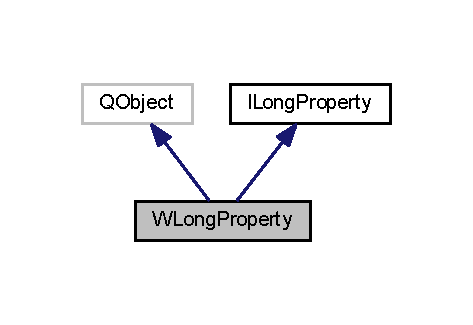
\includegraphics[width=227pt]{class_w_long_property__inherit__graph}
\end{center}
\end{figure}


Collaboration diagram for W\-Long\-Property\-:
\nopagebreak
\begin{figure}[H]
\begin{center}
\leavevmode
\includegraphics[width=229pt]{class_w_long_property__coll__graph}
\end{center}
\end{figure}
\subsection*{Public Slots}
\begin{DoxyCompactItemize}
\item 
void \hyperlink{class_w_long_property_a872aed166209715a26dd676b8b4e7fb4}{set\-Value} (long value)
\begin{DoxyCompactList}\small\item\em Sets the property's value as long . \end{DoxyCompactList}\item 
bool \hyperlink{class_w_long_property_aae809092632e6b8c82cade134d20f89e}{pass\-To} (\hyperlink{class_property_variant}{Property\-Variant} $\ast$variant)
\begin{DoxyCompactList}\small\item\em Passes the property's value to the variant. \end{DoxyCompactList}\end{DoxyCompactItemize}
\subsection*{Public Member Functions}
\begin{DoxyCompactItemize}
\item 
\hyperlink{class_w_long_property_af8f2e6601d3bfd7a70a9f061bdb19fb3}{W\-Long\-Property} (Q\-Object $\ast$parent=0)
\begin{DoxyCompactList}\small\item\em Constructor. Pass the object which implements the interface as parent. \end{DoxyCompactList}\item 
long \hyperlink{class_w_long_property_a2832bb647a51aa6688d4323e44254314}{get\-Value} (bool $\ast$success) const 
\begin{DoxyCompactList}\small\item\em Gets this property's value as long . \end{DoxyCompactList}\item 
bool \hyperlink{class_w_long_property_af0761e534c58bf6b41776dc1298daf8a}{can\-Convert} () const 
\begin{DoxyCompactList}\small\item\em Returns whether or not the property's value can be successfully converted. \end{DoxyCompactList}\end{DoxyCompactItemize}
\subsection*{Protected Attributes}
\begin{DoxyCompactItemize}
\item 
\hyperlink{class_i_long_property}{I\-Long\-Property} $\ast$ \hyperlink{class_w_long_property_aa2f15d5d8e88e1410664fec29b18dea6}{m\-\_\-\-Interface}
\end{DoxyCompactItemize}


\subsection{Detailed Description}
M\-A\-C\-R\-O P\-R\-O\-P\-E\-R\-T\-Y I\-N\-T\-E\-R\-F\-A\-C\-E W\-R\-A\-P\-P\-E\-R F\-O\-R \hyperlink{class_i_long_property}{I\-Long\-Property} . 

Wrapper for the \hyperlink{class_i_long_property}{I\-Long\-Property} interface that facilitates binding of slots to the main class. 

\subsection{Constructor \& Destructor Documentation}
\hypertarget{class_w_long_property_af8f2e6601d3bfd7a70a9f061bdb19fb3}{\index{W\-Long\-Property@{W\-Long\-Property}!W\-Long\-Property@{W\-Long\-Property}}
\index{W\-Long\-Property@{W\-Long\-Property}!WLongProperty@{W\-Long\-Property}}
\subsubsection[{W\-Long\-Property}]{\setlength{\rightskip}{0pt plus 5cm}W\-Long\-Property\-::\-W\-Long\-Property (
\begin{DoxyParamCaption}
\item[{Q\-Object $\ast$}]{parent = {\ttfamily 0}}
\end{DoxyParamCaption}
)\hspace{0.3cm}{\ttfamily [inline]}}}\label{class_w_long_property_af8f2e6601d3bfd7a70a9f061bdb19fb3}


Constructor. Pass the object which implements the interface as parent. 


\begin{DoxyParams}{Parameters}
{\em parent} & Object who implements \hyperlink{class_i_long_property}{I\-Long\-Property} and whose functions this wrapper should bind slots to. \\
\hline
\end{DoxyParams}


\subsection{Member Function Documentation}
\hypertarget{class_w_long_property_af0761e534c58bf6b41776dc1298daf8a}{\index{W\-Long\-Property@{W\-Long\-Property}!can\-Convert@{can\-Convert}}
\index{can\-Convert@{can\-Convert}!WLongProperty@{W\-Long\-Property}}
\subsubsection[{can\-Convert}]{\setlength{\rightskip}{0pt plus 5cm}bool W\-Long\-Property\-::can\-Convert (
\begin{DoxyParamCaption}
{}
\end{DoxyParamCaption}
) const\hspace{0.3cm}{\ttfamily [inline]}, {\ttfamily [virtual]}}}\label{class_w_long_property_af0761e534c58bf6b41776dc1298daf8a}


Returns whether or not the property's value can be successfully converted. 

\begin{DoxyReturn}{Returns}
True if conversion is possible, false otherwise. 
\end{DoxyReturn}


Implements \hyperlink{class_i_long_property_ad6eb15873636142deab4423de11e1ef8}{I\-Long\-Property}.

\hypertarget{class_w_long_property_a2832bb647a51aa6688d4323e44254314}{\index{W\-Long\-Property@{W\-Long\-Property}!get\-Value@{get\-Value}}
\index{get\-Value@{get\-Value}!WLongProperty@{W\-Long\-Property}}
\subsubsection[{get\-Value}]{\setlength{\rightskip}{0pt plus 5cm}long W\-Long\-Property\-::get\-Value (
\begin{DoxyParamCaption}
\item[{bool $\ast$}]{success}
\end{DoxyParamCaption}
) const\hspace{0.3cm}{\ttfamily [inline]}, {\ttfamily [virtual]}}}\label{class_w_long_property_a2832bb647a51aa6688d4323e44254314}


Gets this property's value as long . 


\begin{DoxyParams}{Parameters}
{\em success} & True if conversion was successful, false otherwise.\\
\hline
\end{DoxyParams}
\begin{DoxyReturn}{Returns}
The property's value. 
\end{DoxyReturn}


Implements \hyperlink{class_i_long_property_a52a9796a321b4453f1162fe46746bbcd}{I\-Long\-Property}.

\hypertarget{class_w_long_property_aae809092632e6b8c82cade134d20f89e}{\index{W\-Long\-Property@{W\-Long\-Property}!pass\-To@{pass\-To}}
\index{pass\-To@{pass\-To}!WLongProperty@{W\-Long\-Property}}
\subsubsection[{pass\-To}]{\setlength{\rightskip}{0pt plus 5cm}bool W\-Long\-Property\-::pass\-To (
\begin{DoxyParamCaption}
\item[{{\bf Property\-Variant} $\ast$}]{variant}
\end{DoxyParamCaption}
)\hspace{0.3cm}{\ttfamily [inline]}, {\ttfamily [slot]}}}\label{class_w_long_property_aae809092632e6b8c82cade134d20f89e}


Passes the property's value to the variant. 


\begin{DoxyParams}{Parameters}
{\em variant} & Variant to pass to.\\
\hline
\end{DoxyParams}
\begin{DoxyReturn}{Returns}
True if conversion succeeded, false otherwise. 
\end{DoxyReturn}
\hypertarget{class_w_long_property_a872aed166209715a26dd676b8b4e7fb4}{\index{W\-Long\-Property@{W\-Long\-Property}!set\-Value@{set\-Value}}
\index{set\-Value@{set\-Value}!WLongProperty@{W\-Long\-Property}}
\subsubsection[{set\-Value}]{\setlength{\rightskip}{0pt plus 5cm}void W\-Long\-Property\-::set\-Value (
\begin{DoxyParamCaption}
\item[{long}]{value}
\end{DoxyParamCaption}
)\hspace{0.3cm}{\ttfamily [inline]}, {\ttfamily [slot]}}}\label{class_w_long_property_a872aed166209715a26dd676b8b4e7fb4}


Sets the property's value as long . 


\begin{DoxyParams}{Parameters}
{\em value} & Value to set. \\
\hline
\end{DoxyParams}


\subsection{Member Data Documentation}
\hypertarget{class_w_long_property_aa2f15d5d8e88e1410664fec29b18dea6}{\index{W\-Long\-Property@{W\-Long\-Property}!m\-\_\-\-Interface@{m\-\_\-\-Interface}}
\index{m\-\_\-\-Interface@{m\-\_\-\-Interface}!WLongProperty@{W\-Long\-Property}}
\subsubsection[{m\-\_\-\-Interface}]{\setlength{\rightskip}{0pt plus 5cm}{\bf I\-Long\-Property}$\ast$ W\-Long\-Property\-::m\-\_\-\-Interface\hspace{0.3cm}{\ttfamily [protected]}}}\label{class_w_long_property_aa2f15d5d8e88e1410664fec29b18dea6}
The interface that represents the bound functions on the parent object. 

The documentation for this class was generated from the following file\-:\begin{DoxyCompactItemize}
\item 
app/\hyperlink{property_8h}{property.\-h}\end{DoxyCompactItemize}

\hypertarget{class_w_string_property}{\section{W\-String\-Property Class Reference}
\label{class_w_string_property}\index{W\-String\-Property@{W\-String\-Property}}
}


M\-A\-C\-R\-O P\-R\-O\-P\-E\-R\-T\-Y I\-N\-T\-E\-R\-F\-A\-C\-E W\-R\-A\-P\-P\-E\-R F\-O\-R \hyperlink{class_i_string_property}{I\-String\-Property} .  




{\ttfamily \#include $<$property.\-h$>$}



Inheritance diagram for W\-String\-Property\-:
\nopagebreak
\begin{figure}[H]
\begin{center}
\leavevmode
\includegraphics[width=231pt]{class_w_string_property__inherit__graph}
\end{center}
\end{figure}


Collaboration diagram for W\-String\-Property\-:
\nopagebreak
\begin{figure}[H]
\begin{center}
\leavevmode
\includegraphics[width=231pt]{class_w_string_property__coll__graph}
\end{center}
\end{figure}
\subsection*{Public Slots}
\begin{DoxyCompactItemize}
\item 
void \hyperlink{class_w_string_property_a009c775b69f7365fac0e301ce7d88d2b}{set\-Value} (Q\-String value)
\begin{DoxyCompactList}\small\item\em Sets the property's value as Q\-String . \end{DoxyCompactList}\item 
bool \hyperlink{class_w_string_property_abb5585ce99204a46fb14a5b8cd41ef42}{pass\-To} (\hyperlink{class_property_variant}{Property\-Variant} $\ast$variant)
\begin{DoxyCompactList}\small\item\em Passes the property's value to the variant. \end{DoxyCompactList}\end{DoxyCompactItemize}
\subsection*{Public Member Functions}
\begin{DoxyCompactItemize}
\item 
\hyperlink{class_w_string_property_a228ffc3c7c49e3964e0ed7d59d4e30dd}{W\-String\-Property} (Q\-Object $\ast$parent=0)
\begin{DoxyCompactList}\small\item\em Constructor. Pass the object which implements the interface as parent. \end{DoxyCompactList}\item 
Q\-String \hyperlink{class_w_string_property_a4f31475a4b8cd8f7958bbfdaba6cca42}{get\-Value} (bool $\ast$success) const 
\begin{DoxyCompactList}\small\item\em Gets this property's value as Q\-String . \end{DoxyCompactList}\item 
bool \hyperlink{class_w_string_property_a6b52241cfefcea196a347bc90f57dc25}{can\-Convert} () const 
\begin{DoxyCompactList}\small\item\em Returns whether or not the property's value can be successfully converted. \end{DoxyCompactList}\end{DoxyCompactItemize}
\subsection*{Protected Attributes}
\begin{DoxyCompactItemize}
\item 
\hyperlink{class_i_string_property}{I\-String\-Property} $\ast$ \hyperlink{class_w_string_property_a2a678d70f25fed457ee88e4b1ff85b68}{m\-\_\-\-Interface}
\end{DoxyCompactItemize}


\subsection{Detailed Description}
M\-A\-C\-R\-O P\-R\-O\-P\-E\-R\-T\-Y I\-N\-T\-E\-R\-F\-A\-C\-E W\-R\-A\-P\-P\-E\-R F\-O\-R \hyperlink{class_i_string_property}{I\-String\-Property} . 

Wrapper for the \hyperlink{class_i_string_property}{I\-String\-Property} interface that facilitates binding of slots to the main class. 

\subsection{Constructor \& Destructor Documentation}
\hypertarget{class_w_string_property_a228ffc3c7c49e3964e0ed7d59d4e30dd}{\index{W\-String\-Property@{W\-String\-Property}!W\-String\-Property@{W\-String\-Property}}
\index{W\-String\-Property@{W\-String\-Property}!WStringProperty@{W\-String\-Property}}
\subsubsection[{W\-String\-Property}]{\setlength{\rightskip}{0pt plus 5cm}W\-String\-Property\-::\-W\-String\-Property (
\begin{DoxyParamCaption}
\item[{Q\-Object $\ast$}]{parent = {\ttfamily 0}}
\end{DoxyParamCaption}
)\hspace{0.3cm}{\ttfamily [inline]}}}\label{class_w_string_property_a228ffc3c7c49e3964e0ed7d59d4e30dd}


Constructor. Pass the object which implements the interface as parent. 


\begin{DoxyParams}{Parameters}
{\em parent} & Object who implements \hyperlink{class_i_string_property}{I\-String\-Property} and whose functions this wrapper should bind slots to. \\
\hline
\end{DoxyParams}


\subsection{Member Function Documentation}
\hypertarget{class_w_string_property_a6b52241cfefcea196a347bc90f57dc25}{\index{W\-String\-Property@{W\-String\-Property}!can\-Convert@{can\-Convert}}
\index{can\-Convert@{can\-Convert}!WStringProperty@{W\-String\-Property}}
\subsubsection[{can\-Convert}]{\setlength{\rightskip}{0pt plus 5cm}bool W\-String\-Property\-::can\-Convert (
\begin{DoxyParamCaption}
{}
\end{DoxyParamCaption}
) const\hspace{0.3cm}{\ttfamily [inline]}, {\ttfamily [virtual]}}}\label{class_w_string_property_a6b52241cfefcea196a347bc90f57dc25}


Returns whether or not the property's value can be successfully converted. 

\begin{DoxyReturn}{Returns}
True if conversion is possible, false otherwise. 
\end{DoxyReturn}


Implements \hyperlink{class_i_string_property_a2fcab392710db1ae140e394c1db6739e}{I\-String\-Property}.

\hypertarget{class_w_string_property_a4f31475a4b8cd8f7958bbfdaba6cca42}{\index{W\-String\-Property@{W\-String\-Property}!get\-Value@{get\-Value}}
\index{get\-Value@{get\-Value}!WStringProperty@{W\-String\-Property}}
\subsubsection[{get\-Value}]{\setlength{\rightskip}{0pt plus 5cm}Q\-String W\-String\-Property\-::get\-Value (
\begin{DoxyParamCaption}
\item[{bool $\ast$}]{success}
\end{DoxyParamCaption}
) const\hspace{0.3cm}{\ttfamily [inline]}, {\ttfamily [virtual]}}}\label{class_w_string_property_a4f31475a4b8cd8f7958bbfdaba6cca42}


Gets this property's value as Q\-String . 


\begin{DoxyParams}{Parameters}
{\em success} & True if conversion was successful, false otherwise.\\
\hline
\end{DoxyParams}
\begin{DoxyReturn}{Returns}
The property's value. 
\end{DoxyReturn}


Implements \hyperlink{class_i_string_property_a0dbe79993973e018510325120762504f}{I\-String\-Property}.

\hypertarget{class_w_string_property_abb5585ce99204a46fb14a5b8cd41ef42}{\index{W\-String\-Property@{W\-String\-Property}!pass\-To@{pass\-To}}
\index{pass\-To@{pass\-To}!WStringProperty@{W\-String\-Property}}
\subsubsection[{pass\-To}]{\setlength{\rightskip}{0pt plus 5cm}bool W\-String\-Property\-::pass\-To (
\begin{DoxyParamCaption}
\item[{{\bf Property\-Variant} $\ast$}]{variant}
\end{DoxyParamCaption}
)\hspace{0.3cm}{\ttfamily [inline]}, {\ttfamily [slot]}}}\label{class_w_string_property_abb5585ce99204a46fb14a5b8cd41ef42}


Passes the property's value to the variant. 


\begin{DoxyParams}{Parameters}
{\em variant} & Variant to pass to.\\
\hline
\end{DoxyParams}
\begin{DoxyReturn}{Returns}
True if conversion succeeded, false otherwise. 
\end{DoxyReturn}
\hypertarget{class_w_string_property_a009c775b69f7365fac0e301ce7d88d2b}{\index{W\-String\-Property@{W\-String\-Property}!set\-Value@{set\-Value}}
\index{set\-Value@{set\-Value}!WStringProperty@{W\-String\-Property}}
\subsubsection[{set\-Value}]{\setlength{\rightskip}{0pt plus 5cm}void W\-String\-Property\-::set\-Value (
\begin{DoxyParamCaption}
\item[{Q\-String}]{value}
\end{DoxyParamCaption}
)\hspace{0.3cm}{\ttfamily [inline]}, {\ttfamily [slot]}}}\label{class_w_string_property_a009c775b69f7365fac0e301ce7d88d2b}


Sets the property's value as Q\-String . 


\begin{DoxyParams}{Parameters}
{\em value} & Value to set. \\
\hline
\end{DoxyParams}


\subsection{Member Data Documentation}
\hypertarget{class_w_string_property_a2a678d70f25fed457ee88e4b1ff85b68}{\index{W\-String\-Property@{W\-String\-Property}!m\-\_\-\-Interface@{m\-\_\-\-Interface}}
\index{m\-\_\-\-Interface@{m\-\_\-\-Interface}!WStringProperty@{W\-String\-Property}}
\subsubsection[{m\-\_\-\-Interface}]{\setlength{\rightskip}{0pt plus 5cm}{\bf I\-String\-Property}$\ast$ W\-String\-Property\-::m\-\_\-\-Interface\hspace{0.3cm}{\ttfamily [protected]}}}\label{class_w_string_property_a2a678d70f25fed457ee88e4b1ff85b68}
The interface that represents the bound functions on the parent object. 

The documentation for this class was generated from the following file\-:\begin{DoxyCompactItemize}
\item 
app/\hyperlink{property_8h}{property.\-h}\end{DoxyCompactItemize}

\hypertarget{class_w_u_int_property}{\section{W\-U\-Int\-Property Class Reference}
\label{class_w_u_int_property}\index{W\-U\-Int\-Property@{W\-U\-Int\-Property}}
}


M\-A\-C\-R\-O P\-R\-O\-P\-E\-R\-T\-Y I\-N\-T\-E\-R\-F\-A\-C\-E W\-R\-A\-P\-P\-E\-R F\-O\-R \hyperlink{class_i_u_int_property}{I\-U\-Int\-Property} .  




{\ttfamily \#include $<$property.\-h$>$}



Inheritance diagram for W\-U\-Int\-Property\-:
\nopagebreak
\begin{figure}[H]
\begin{center}
\leavevmode
\includegraphics[width=223pt]{class_w_u_int_property__inherit__graph}
\end{center}
\end{figure}


Collaboration diagram for W\-U\-Int\-Property\-:
\nopagebreak
\begin{figure}[H]
\begin{center}
\leavevmode
\includegraphics[width=227pt]{class_w_u_int_property__coll__graph}
\end{center}
\end{figure}
\subsection*{Public Slots}
\begin{DoxyCompactItemize}
\item 
void \hyperlink{class_w_u_int_property_a05e1e1e89a9295007ffea09ea46a0ac4}{set\-Value} (uint value)
\begin{DoxyCompactList}\small\item\em Sets the property's value as uint . \end{DoxyCompactList}\item 
bool \hyperlink{class_w_u_int_property_adad4788a892a0c990d068f10863090d8}{pass\-To} (\hyperlink{class_property_variant}{Property\-Variant} $\ast$variant)
\begin{DoxyCompactList}\small\item\em Passes the property's value to the variant. \end{DoxyCompactList}\end{DoxyCompactItemize}
\subsection*{Public Member Functions}
\begin{DoxyCompactItemize}
\item 
\hyperlink{class_w_u_int_property_a7bd95ff163ad1bf9fcd995aff49919f5}{W\-U\-Int\-Property} (Q\-Object $\ast$parent=0)
\begin{DoxyCompactList}\small\item\em Constructor. Pass the object which implements the interface as parent. \end{DoxyCompactList}\item 
uint \hyperlink{class_w_u_int_property_af79534aa085135c8c642a1e929119147}{get\-Value} (bool $\ast$success) const 
\begin{DoxyCompactList}\small\item\em Gets this property's value as uint . \end{DoxyCompactList}\item 
bool \hyperlink{class_w_u_int_property_a27a4e53bf0702e796c6eecfbe9803221}{can\-Convert} () const 
\begin{DoxyCompactList}\small\item\em Returns whether or not the property's value can be successfully converted. \end{DoxyCompactList}\end{DoxyCompactItemize}
\subsection*{Protected Attributes}
\begin{DoxyCompactItemize}
\item 
\hyperlink{class_i_u_int_property}{I\-U\-Int\-Property} $\ast$ \hyperlink{class_w_u_int_property_aef61d929eea5c2e11c3ccf7e5921f564}{m\-\_\-\-Interface}
\end{DoxyCompactItemize}


\subsection{Detailed Description}
M\-A\-C\-R\-O P\-R\-O\-P\-E\-R\-T\-Y I\-N\-T\-E\-R\-F\-A\-C\-E W\-R\-A\-P\-P\-E\-R F\-O\-R \hyperlink{class_i_u_int_property}{I\-U\-Int\-Property} . 

Wrapper for the \hyperlink{class_i_u_int_property}{I\-U\-Int\-Property} interface that facilitates binding of slots to the main class. 

\subsection{Constructor \& Destructor Documentation}
\hypertarget{class_w_u_int_property_a7bd95ff163ad1bf9fcd995aff49919f5}{\index{W\-U\-Int\-Property@{W\-U\-Int\-Property}!W\-U\-Int\-Property@{W\-U\-Int\-Property}}
\index{W\-U\-Int\-Property@{W\-U\-Int\-Property}!WUIntProperty@{W\-U\-Int\-Property}}
\subsubsection[{W\-U\-Int\-Property}]{\setlength{\rightskip}{0pt plus 5cm}W\-U\-Int\-Property\-::\-W\-U\-Int\-Property (
\begin{DoxyParamCaption}
\item[{Q\-Object $\ast$}]{parent = {\ttfamily 0}}
\end{DoxyParamCaption}
)\hspace{0.3cm}{\ttfamily [inline]}}}\label{class_w_u_int_property_a7bd95ff163ad1bf9fcd995aff49919f5}


Constructor. Pass the object which implements the interface as parent. 


\begin{DoxyParams}{Parameters}
{\em parent} & Object who implements \hyperlink{class_i_u_int_property}{I\-U\-Int\-Property} and whose functions this wrapper should bind slots to. \\
\hline
\end{DoxyParams}


\subsection{Member Function Documentation}
\hypertarget{class_w_u_int_property_a27a4e53bf0702e796c6eecfbe9803221}{\index{W\-U\-Int\-Property@{W\-U\-Int\-Property}!can\-Convert@{can\-Convert}}
\index{can\-Convert@{can\-Convert}!WUIntProperty@{W\-U\-Int\-Property}}
\subsubsection[{can\-Convert}]{\setlength{\rightskip}{0pt plus 5cm}bool W\-U\-Int\-Property\-::can\-Convert (
\begin{DoxyParamCaption}
{}
\end{DoxyParamCaption}
) const\hspace{0.3cm}{\ttfamily [inline]}, {\ttfamily [virtual]}}}\label{class_w_u_int_property_a27a4e53bf0702e796c6eecfbe9803221}


Returns whether or not the property's value can be successfully converted. 

\begin{DoxyReturn}{Returns}
True if conversion is possible, false otherwise. 
\end{DoxyReturn}


Implements \hyperlink{class_i_u_int_property_a4fa6fa9ef5663109772bf51123323c87}{I\-U\-Int\-Property}.

\hypertarget{class_w_u_int_property_af79534aa085135c8c642a1e929119147}{\index{W\-U\-Int\-Property@{W\-U\-Int\-Property}!get\-Value@{get\-Value}}
\index{get\-Value@{get\-Value}!WUIntProperty@{W\-U\-Int\-Property}}
\subsubsection[{get\-Value}]{\setlength{\rightskip}{0pt plus 5cm}uint W\-U\-Int\-Property\-::get\-Value (
\begin{DoxyParamCaption}
\item[{bool $\ast$}]{success}
\end{DoxyParamCaption}
) const\hspace{0.3cm}{\ttfamily [inline]}, {\ttfamily [virtual]}}}\label{class_w_u_int_property_af79534aa085135c8c642a1e929119147}


Gets this property's value as uint . 


\begin{DoxyParams}{Parameters}
{\em success} & True if conversion was successful, false otherwise.\\
\hline
\end{DoxyParams}
\begin{DoxyReturn}{Returns}
The property's value. 
\end{DoxyReturn}


Implements \hyperlink{class_i_u_int_property_af3c17d292a74241f1d80b10be434edde}{I\-U\-Int\-Property}.

\hypertarget{class_w_u_int_property_adad4788a892a0c990d068f10863090d8}{\index{W\-U\-Int\-Property@{W\-U\-Int\-Property}!pass\-To@{pass\-To}}
\index{pass\-To@{pass\-To}!WUIntProperty@{W\-U\-Int\-Property}}
\subsubsection[{pass\-To}]{\setlength{\rightskip}{0pt plus 5cm}bool W\-U\-Int\-Property\-::pass\-To (
\begin{DoxyParamCaption}
\item[{{\bf Property\-Variant} $\ast$}]{variant}
\end{DoxyParamCaption}
)\hspace{0.3cm}{\ttfamily [inline]}, {\ttfamily [slot]}}}\label{class_w_u_int_property_adad4788a892a0c990d068f10863090d8}


Passes the property's value to the variant. 


\begin{DoxyParams}{Parameters}
{\em variant} & Variant to pass to.\\
\hline
\end{DoxyParams}
\begin{DoxyReturn}{Returns}
True if conversion succeeded, false otherwise. 
\end{DoxyReturn}
\hypertarget{class_w_u_int_property_a05e1e1e89a9295007ffea09ea46a0ac4}{\index{W\-U\-Int\-Property@{W\-U\-Int\-Property}!set\-Value@{set\-Value}}
\index{set\-Value@{set\-Value}!WUIntProperty@{W\-U\-Int\-Property}}
\subsubsection[{set\-Value}]{\setlength{\rightskip}{0pt plus 5cm}void W\-U\-Int\-Property\-::set\-Value (
\begin{DoxyParamCaption}
\item[{uint}]{value}
\end{DoxyParamCaption}
)\hspace{0.3cm}{\ttfamily [inline]}, {\ttfamily [slot]}}}\label{class_w_u_int_property_a05e1e1e89a9295007ffea09ea46a0ac4}


Sets the property's value as uint . 


\begin{DoxyParams}{Parameters}
{\em value} & Value to set. \\
\hline
\end{DoxyParams}


\subsection{Member Data Documentation}
\hypertarget{class_w_u_int_property_aef61d929eea5c2e11c3ccf7e5921f564}{\index{W\-U\-Int\-Property@{W\-U\-Int\-Property}!m\-\_\-\-Interface@{m\-\_\-\-Interface}}
\index{m\-\_\-\-Interface@{m\-\_\-\-Interface}!WUIntProperty@{W\-U\-Int\-Property}}
\subsubsection[{m\-\_\-\-Interface}]{\setlength{\rightskip}{0pt plus 5cm}{\bf I\-U\-Int\-Property}$\ast$ W\-U\-Int\-Property\-::m\-\_\-\-Interface\hspace{0.3cm}{\ttfamily [protected]}}}\label{class_w_u_int_property_aef61d929eea5c2e11c3ccf7e5921f564}
The interface that represents the bound functions on the parent object. 

The documentation for this class was generated from the following file\-:\begin{DoxyCompactItemize}
\item 
app/\hyperlink{property_8h}{property.\-h}\end{DoxyCompactItemize}

\hypertarget{class_w_u_long_long_property}{\section{W\-U\-Long\-Long\-Property Class Reference}
\label{class_w_u_long_long_property}\index{W\-U\-Long\-Long\-Property@{W\-U\-Long\-Long\-Property}}
}


M\-A\-C\-R\-O P\-R\-O\-P\-E\-R\-T\-Y I\-N\-T\-E\-R\-F\-A\-C\-E W\-R\-A\-P\-P\-E\-R F\-O\-R \hyperlink{class_i_u_long_long_property}{I\-U\-Long\-Long\-Property} .  




{\ttfamily \#include $<$property.\-h$>$}



Inheritance diagram for W\-U\-Long\-Long\-Property\-:
\nopagebreak
\begin{figure}[H]
\begin{center}
\leavevmode
\includegraphics[width=255pt]{class_w_u_long_long_property__inherit__graph}
\end{center}
\end{figure}


Collaboration diagram for W\-U\-Long\-Long\-Property\-:
\nopagebreak
\begin{figure}[H]
\begin{center}
\leavevmode
\includegraphics[width=255pt]{class_w_u_long_long_property__coll__graph}
\end{center}
\end{figure}
\subsection*{Public Slots}
\begin{DoxyCompactItemize}
\item 
void \hyperlink{class_w_u_long_long_property_a88fb26420c3f7472f4499a7701ff9fc2}{set\-Value} (qulonglong value)
\begin{DoxyCompactList}\small\item\em Sets the property's value as qulonglong . \end{DoxyCompactList}\item 
bool \hyperlink{class_w_u_long_long_property_a080691c54190a03952b451b346541a86}{pass\-To} (\hyperlink{class_property_variant}{Property\-Variant} $\ast$variant)
\begin{DoxyCompactList}\small\item\em Passes the property's value to the variant. \end{DoxyCompactList}\end{DoxyCompactItemize}
\subsection*{Public Member Functions}
\begin{DoxyCompactItemize}
\item 
\hyperlink{class_w_u_long_long_property_a6f66a9a2fb1b6157a7dab9e721511235}{W\-U\-Long\-Long\-Property} (Q\-Object $\ast$parent=0)
\begin{DoxyCompactList}\small\item\em Constructor. Pass the object which implements the interface as parent. \end{DoxyCompactList}\item 
qulonglong \hyperlink{class_w_u_long_long_property_aca6d125f5a4cd021ba353c2afd5ca31d}{get\-Value} (bool $\ast$success) const 
\begin{DoxyCompactList}\small\item\em Gets this property's value as qulonglong . \end{DoxyCompactList}\item 
bool \hyperlink{class_w_u_long_long_property_a35c48d980e5e28944a9521e80e89e592}{can\-Convert} () const 
\begin{DoxyCompactList}\small\item\em Returns whether or not the property's value can be successfully converted. \end{DoxyCompactList}\end{DoxyCompactItemize}
\subsection*{Protected Attributes}
\begin{DoxyCompactItemize}
\item 
\hyperlink{class_i_u_long_long_property}{I\-U\-Long\-Long\-Property} $\ast$ \hyperlink{class_w_u_long_long_property_af84b2abd75425a2173ed9450c2a65ce6}{m\-\_\-\-Interface}
\end{DoxyCompactItemize}


\subsection{Detailed Description}
M\-A\-C\-R\-O P\-R\-O\-P\-E\-R\-T\-Y I\-N\-T\-E\-R\-F\-A\-C\-E W\-R\-A\-P\-P\-E\-R F\-O\-R \hyperlink{class_i_u_long_long_property}{I\-U\-Long\-Long\-Property} . 

Wrapper for the \hyperlink{class_i_u_long_long_property}{I\-U\-Long\-Long\-Property} interface that facilitates binding of slots to the main class. 

\subsection{Constructor \& Destructor Documentation}
\hypertarget{class_w_u_long_long_property_a6f66a9a2fb1b6157a7dab9e721511235}{\index{W\-U\-Long\-Long\-Property@{W\-U\-Long\-Long\-Property}!W\-U\-Long\-Long\-Property@{W\-U\-Long\-Long\-Property}}
\index{W\-U\-Long\-Long\-Property@{W\-U\-Long\-Long\-Property}!WULongLongProperty@{W\-U\-Long\-Long\-Property}}
\subsubsection[{W\-U\-Long\-Long\-Property}]{\setlength{\rightskip}{0pt plus 5cm}W\-U\-Long\-Long\-Property\-::\-W\-U\-Long\-Long\-Property (
\begin{DoxyParamCaption}
\item[{Q\-Object $\ast$}]{parent = {\ttfamily 0}}
\end{DoxyParamCaption}
)\hspace{0.3cm}{\ttfamily [inline]}}}\label{class_w_u_long_long_property_a6f66a9a2fb1b6157a7dab9e721511235}


Constructor. Pass the object which implements the interface as parent. 


\begin{DoxyParams}{Parameters}
{\em parent} & Object who implements \hyperlink{class_i_u_long_long_property}{I\-U\-Long\-Long\-Property} and whose functions this wrapper should bind slots to. \\
\hline
\end{DoxyParams}


\subsection{Member Function Documentation}
\hypertarget{class_w_u_long_long_property_a35c48d980e5e28944a9521e80e89e592}{\index{W\-U\-Long\-Long\-Property@{W\-U\-Long\-Long\-Property}!can\-Convert@{can\-Convert}}
\index{can\-Convert@{can\-Convert}!WULongLongProperty@{W\-U\-Long\-Long\-Property}}
\subsubsection[{can\-Convert}]{\setlength{\rightskip}{0pt plus 5cm}bool W\-U\-Long\-Long\-Property\-::can\-Convert (
\begin{DoxyParamCaption}
{}
\end{DoxyParamCaption}
) const\hspace{0.3cm}{\ttfamily [inline]}, {\ttfamily [virtual]}}}\label{class_w_u_long_long_property_a35c48d980e5e28944a9521e80e89e592}


Returns whether or not the property's value can be successfully converted. 

\begin{DoxyReturn}{Returns}
True if conversion is possible, false otherwise. 
\end{DoxyReturn}


Implements \hyperlink{class_i_u_long_long_property_a905e766d258ebf63ed683a32aa2427a0}{I\-U\-Long\-Long\-Property}.

\hypertarget{class_w_u_long_long_property_aca6d125f5a4cd021ba353c2afd5ca31d}{\index{W\-U\-Long\-Long\-Property@{W\-U\-Long\-Long\-Property}!get\-Value@{get\-Value}}
\index{get\-Value@{get\-Value}!WULongLongProperty@{W\-U\-Long\-Long\-Property}}
\subsubsection[{get\-Value}]{\setlength{\rightskip}{0pt plus 5cm}qulonglong W\-U\-Long\-Long\-Property\-::get\-Value (
\begin{DoxyParamCaption}
\item[{bool $\ast$}]{success}
\end{DoxyParamCaption}
) const\hspace{0.3cm}{\ttfamily [inline]}, {\ttfamily [virtual]}}}\label{class_w_u_long_long_property_aca6d125f5a4cd021ba353c2afd5ca31d}


Gets this property's value as qulonglong . 


\begin{DoxyParams}{Parameters}
{\em success} & True if conversion was successful, false otherwise.\\
\hline
\end{DoxyParams}
\begin{DoxyReturn}{Returns}
The property's value. 
\end{DoxyReturn}


Implements \hyperlink{class_i_u_long_long_property_acddc945a90cac8fa5921a9be25aaed13}{I\-U\-Long\-Long\-Property}.

\hypertarget{class_w_u_long_long_property_a080691c54190a03952b451b346541a86}{\index{W\-U\-Long\-Long\-Property@{W\-U\-Long\-Long\-Property}!pass\-To@{pass\-To}}
\index{pass\-To@{pass\-To}!WULongLongProperty@{W\-U\-Long\-Long\-Property}}
\subsubsection[{pass\-To}]{\setlength{\rightskip}{0pt plus 5cm}bool W\-U\-Long\-Long\-Property\-::pass\-To (
\begin{DoxyParamCaption}
\item[{{\bf Property\-Variant} $\ast$}]{variant}
\end{DoxyParamCaption}
)\hspace{0.3cm}{\ttfamily [inline]}, {\ttfamily [slot]}}}\label{class_w_u_long_long_property_a080691c54190a03952b451b346541a86}


Passes the property's value to the variant. 


\begin{DoxyParams}{Parameters}
{\em variant} & Variant to pass to.\\
\hline
\end{DoxyParams}
\begin{DoxyReturn}{Returns}
True if conversion succeeded, false otherwise. 
\end{DoxyReturn}
\hypertarget{class_w_u_long_long_property_a88fb26420c3f7472f4499a7701ff9fc2}{\index{W\-U\-Long\-Long\-Property@{W\-U\-Long\-Long\-Property}!set\-Value@{set\-Value}}
\index{set\-Value@{set\-Value}!WULongLongProperty@{W\-U\-Long\-Long\-Property}}
\subsubsection[{set\-Value}]{\setlength{\rightskip}{0pt plus 5cm}void W\-U\-Long\-Long\-Property\-::set\-Value (
\begin{DoxyParamCaption}
\item[{qulonglong}]{value}
\end{DoxyParamCaption}
)\hspace{0.3cm}{\ttfamily [inline]}, {\ttfamily [slot]}}}\label{class_w_u_long_long_property_a88fb26420c3f7472f4499a7701ff9fc2}


Sets the property's value as qulonglong . 


\begin{DoxyParams}{Parameters}
{\em value} & Value to set. \\
\hline
\end{DoxyParams}


\subsection{Member Data Documentation}
\hypertarget{class_w_u_long_long_property_af84b2abd75425a2173ed9450c2a65ce6}{\index{W\-U\-Long\-Long\-Property@{W\-U\-Long\-Long\-Property}!m\-\_\-\-Interface@{m\-\_\-\-Interface}}
\index{m\-\_\-\-Interface@{m\-\_\-\-Interface}!WULongLongProperty@{W\-U\-Long\-Long\-Property}}
\subsubsection[{m\-\_\-\-Interface}]{\setlength{\rightskip}{0pt plus 5cm}{\bf I\-U\-Long\-Long\-Property}$\ast$ W\-U\-Long\-Long\-Property\-::m\-\_\-\-Interface\hspace{0.3cm}{\ttfamily [protected]}}}\label{class_w_u_long_long_property_af84b2abd75425a2173ed9450c2a65ce6}
The interface that represents the bound functions on the parent object. 

The documentation for this class was generated from the following file\-:\begin{DoxyCompactItemize}
\item 
app/\hyperlink{property_8h}{property.\-h}\end{DoxyCompactItemize}

\hypertarget{class_w_u_long_property}{\section{W\-U\-Long\-Property Class Reference}
\label{class_w_u_long_property}\index{W\-U\-Long\-Property@{W\-U\-Long\-Property}}
}


M\-A\-C\-R\-O P\-R\-O\-P\-E\-R\-T\-Y I\-N\-T\-E\-R\-F\-A\-C\-E W\-R\-A\-P\-P\-E\-R F\-O\-R \hyperlink{class_i_u_long_property}{I\-U\-Long\-Property} .  




{\ttfamily \#include $<$property.\-h$>$}



Inheritance diagram for W\-U\-Long\-Property\-:
\nopagebreak
\begin{figure}[H]
\begin{center}
\leavevmode
\includegraphics[width=233pt]{class_w_u_long_property__inherit__graph}
\end{center}
\end{figure}


Collaboration diagram for W\-U\-Long\-Property\-:
\nopagebreak
\begin{figure}[H]
\begin{center}
\leavevmode
\includegraphics[width=233pt]{class_w_u_long_property__coll__graph}
\end{center}
\end{figure}
\subsection*{Public Slots}
\begin{DoxyCompactItemize}
\item 
void \hyperlink{class_w_u_long_property_a9536e4c79e6a9aa6536b6c3e26638bea}{set\-Value} (ulong value)
\begin{DoxyCompactList}\small\item\em Sets the property's value as ulong . \end{DoxyCompactList}\end{DoxyCompactItemize}
\subsection*{Public Member Functions}
\begin{DoxyCompactItemize}
\item 
\hyperlink{class_w_u_long_property_ab2e17ffa240a20e21098ad95ba202260}{W\-U\-Long\-Property} (Q\-Object $\ast$parent=0)
\begin{DoxyCompactList}\small\item\em Constructor. Pass the object which implements the interface as parent. \end{DoxyCompactList}\item 
\hyperlink{group___property_classes_ga38f1ccddda12c7cb50b868c9f789ee37}{Property\-\_\-t} \hyperlink{class_w_u_long_property_a1540e17406836973ff4ffedc7ea7d294}{get\-Property\-Type} () const 
\begin{DoxyCompactList}\small\item\em Returns the Property\-\_\-t to classify this property. \end{DoxyCompactList}\item 
ulong \hyperlink{class_w_u_long_property_a58823102ac77872b7700b0e4347cac28}{get\-Value} (bool $\ast$success) const 
\begin{DoxyCompactList}\small\item\em Gets this property's value as ulong . \end{DoxyCompactList}\item 
bool \hyperlink{class_w_u_long_property_add1989192edb81ac284a6680cf9f32dd}{can\-Convert} () const 
\begin{DoxyCompactList}\small\item\em Returns whether or not the property's value can be successfully converted. \end{DoxyCompactList}\end{DoxyCompactItemize}
\subsection*{Protected Attributes}
\begin{DoxyCompactItemize}
\item 
\hyperlink{class_i_u_long_property}{I\-U\-Long\-Property} $\ast$ \hyperlink{class_w_u_long_property_ae67a466defe432cdd559c753dc02a5a0}{m\-\_\-\-Interface}
\end{DoxyCompactItemize}


\subsection{Detailed Description}
M\-A\-C\-R\-O P\-R\-O\-P\-E\-R\-T\-Y I\-N\-T\-E\-R\-F\-A\-C\-E W\-R\-A\-P\-P\-E\-R F\-O\-R \hyperlink{class_i_u_long_property}{I\-U\-Long\-Property} . 

Wrapper for the \hyperlink{class_i_u_long_property}{I\-U\-Long\-Property} interface that facilitates binding of slots to the main class. 

\subsection{Constructor \& Destructor Documentation}
\hypertarget{class_w_u_long_property_ab2e17ffa240a20e21098ad95ba202260}{\index{W\-U\-Long\-Property@{W\-U\-Long\-Property}!W\-U\-Long\-Property@{W\-U\-Long\-Property}}
\index{W\-U\-Long\-Property@{W\-U\-Long\-Property}!WULongProperty@{W\-U\-Long\-Property}}
\subsubsection[{W\-U\-Long\-Property}]{\setlength{\rightskip}{0pt plus 5cm}W\-U\-Long\-Property\-::\-W\-U\-Long\-Property (
\begin{DoxyParamCaption}
\item[{Q\-Object $\ast$}]{parent = {\ttfamily 0}}
\end{DoxyParamCaption}
)\hspace{0.3cm}{\ttfamily [inline]}}}\label{class_w_u_long_property_ab2e17ffa240a20e21098ad95ba202260}


Constructor. Pass the object which implements the interface as parent. 


\begin{DoxyParams}{Parameters}
{\em parent} & Object who implements \hyperlink{class_i_u_long_property}{I\-U\-Long\-Property} and whose functions this wrapper should bind slots to. \\
\hline
\end{DoxyParams}


\subsection{Member Function Documentation}
\hypertarget{class_w_u_long_property_add1989192edb81ac284a6680cf9f32dd}{\index{W\-U\-Long\-Property@{W\-U\-Long\-Property}!can\-Convert@{can\-Convert}}
\index{can\-Convert@{can\-Convert}!WULongProperty@{W\-U\-Long\-Property}}
\subsubsection[{can\-Convert}]{\setlength{\rightskip}{0pt plus 5cm}bool W\-U\-Long\-Property\-::can\-Convert (
\begin{DoxyParamCaption}
{}
\end{DoxyParamCaption}
) const\hspace{0.3cm}{\ttfamily [inline]}, {\ttfamily [virtual]}}}\label{class_w_u_long_property_add1989192edb81ac284a6680cf9f32dd}


Returns whether or not the property's value can be successfully converted. 

\begin{DoxyReturn}{Returns}
True if conversion is possible, false otherwise. 
\end{DoxyReturn}


Implements \hyperlink{class_i_u_long_property_ad63c658df7494298fd8a0ab41623a184}{I\-U\-Long\-Property}.

\hypertarget{class_w_u_long_property_a1540e17406836973ff4ffedc7ea7d294}{\index{W\-U\-Long\-Property@{W\-U\-Long\-Property}!get\-Property\-Type@{get\-Property\-Type}}
\index{get\-Property\-Type@{get\-Property\-Type}!WULongProperty@{W\-U\-Long\-Property}}
\subsubsection[{get\-Property\-Type}]{\setlength{\rightskip}{0pt plus 5cm}{\bf Property\-\_\-t} W\-U\-Long\-Property\-::get\-Property\-Type (
\begin{DoxyParamCaption}
{}
\end{DoxyParamCaption}
) const\hspace{0.3cm}{\ttfamily [inline]}, {\ttfamily [virtual]}}}\label{class_w_u_long_property_a1540e17406836973ff4ffedc7ea7d294}


Returns the Property\-\_\-t to classify this property. 

\begin{DoxyReturn}{Returns}
Property\-\_\-t classifier. 
\end{DoxyReturn}


Implements \hyperlink{class_i_u_long_property_afcabc7c115954f9619eb2d519de1c83e}{I\-U\-Long\-Property}.

\hypertarget{class_w_u_long_property_a58823102ac77872b7700b0e4347cac28}{\index{W\-U\-Long\-Property@{W\-U\-Long\-Property}!get\-Value@{get\-Value}}
\index{get\-Value@{get\-Value}!WULongProperty@{W\-U\-Long\-Property}}
\subsubsection[{get\-Value}]{\setlength{\rightskip}{0pt plus 5cm}ulong W\-U\-Long\-Property\-::get\-Value (
\begin{DoxyParamCaption}
\item[{bool $\ast$}]{success}
\end{DoxyParamCaption}
) const\hspace{0.3cm}{\ttfamily [inline]}, {\ttfamily [virtual]}}}\label{class_w_u_long_property_a58823102ac77872b7700b0e4347cac28}


Gets this property's value as ulong . 


\begin{DoxyParams}{Parameters}
{\em success} & True if conversion was successful, false otherwise.\\
\hline
\end{DoxyParams}
\begin{DoxyReturn}{Returns}
The property's value. 
\end{DoxyReturn}


Implements \hyperlink{class_i_u_long_property_a620e0d9b7260d93ee9e5a55c5c648f92}{I\-U\-Long\-Property}.

\hypertarget{class_w_u_long_property_a9536e4c79e6a9aa6536b6c3e26638bea}{\index{W\-U\-Long\-Property@{W\-U\-Long\-Property}!set\-Value@{set\-Value}}
\index{set\-Value@{set\-Value}!WULongProperty@{W\-U\-Long\-Property}}
\subsubsection[{set\-Value}]{\setlength{\rightskip}{0pt plus 5cm}void W\-U\-Long\-Property\-::set\-Value (
\begin{DoxyParamCaption}
\item[{ulong}]{value}
\end{DoxyParamCaption}
)\hspace{0.3cm}{\ttfamily [inline]}, {\ttfamily [slot]}}}\label{class_w_u_long_property_a9536e4c79e6a9aa6536b6c3e26638bea}


Sets the property's value as ulong . 


\begin{DoxyParams}{Parameters}
{\em value} & Value to set. \\
\hline
\end{DoxyParams}


\subsection{Member Data Documentation}
\hypertarget{class_w_u_long_property_ae67a466defe432cdd559c753dc02a5a0}{\index{W\-U\-Long\-Property@{W\-U\-Long\-Property}!m\-\_\-\-Interface@{m\-\_\-\-Interface}}
\index{m\-\_\-\-Interface@{m\-\_\-\-Interface}!WULongProperty@{W\-U\-Long\-Property}}
\subsubsection[{m\-\_\-\-Interface}]{\setlength{\rightskip}{0pt plus 5cm}{\bf I\-U\-Long\-Property}$\ast$ W\-U\-Long\-Property\-::m\-\_\-\-Interface\hspace{0.3cm}{\ttfamily [protected]}}}\label{class_w_u_long_property_ae67a466defe432cdd559c753dc02a5a0}
The interface that represents the bound functions on the parent object. 

The documentation for this class was generated from the following file\-:\begin{DoxyCompactItemize}
\item 
app/\hyperlink{property_8h}{property.\-h}\end{DoxyCompactItemize}

\chapter{File Documentation}
\hypertarget{baseproperty_8h}{\section{app/baseproperty.h File Reference}
\label{baseproperty_8h}\index{app/baseproperty.\-h@{app/baseproperty.\-h}}
}


Defines the property base class and interfaces.  


{\ttfamily \#include $<$Q\-Object$>$}\\*
{\ttfamily \#include $<$Q\-Pair$>$}\\*
Include dependency graph for baseproperty.\-h\-:
\nopagebreak
\begin{figure}[H]
\begin{center}
\leavevmode
\includegraphics[width=191pt]{baseproperty_8h__incl}
\end{center}
\end{figure}
This graph shows which files directly or indirectly include this file\-:
\nopagebreak
\begin{figure}[H]
\begin{center}
\leavevmode
\includegraphics[width=180pt]{baseproperty_8h__dep__incl}
\end{center}
\end{figure}
\subsection*{Classes}
\begin{DoxyCompactItemize}
\item 
class \hyperlink{class_i_base_property}{I\-Base\-Property}
\begin{DoxyCompactList}\small\item\em Base property interface. \end{DoxyCompactList}\item 
class \hyperlink{class_w_base_property}{W\-Base\-Property}
\begin{DoxyCompactList}\small\item\em Base property interface wrapper. \end{DoxyCompactList}\item 
class \hyperlink{class_base_property}{Base\-Property}
\begin{DoxyCompactList}\small\item\em Base property class. \end{DoxyCompactList}\item 
class \hyperlink{class_i_property_variant}{I\-Property\-Variant}
\begin{DoxyCompactList}\small\item\em Interface implemented by \hyperlink{class_property_variant}{Property\-Variant}. \end{DoxyCompactList}\item 
class \hyperlink{class_w_property_variant}{W\-Property\-Variant}
\begin{DoxyCompactList}\small\item\em \hyperlink{class_property_variant}{Property\-Variant} interface wrapper. \end{DoxyCompactList}\item 
class \hyperlink{class_property_variant}{Property\-Variant}
\begin{DoxyCompactList}\small\item\em Allows fetching of subclassed properties from a list of \hyperlink{class_base_property}{Base\-Property} pointers. \end{DoxyCompactList}\end{DoxyCompactItemize}
\subsection*{Macros}
\begin{DoxyCompactItemize}
\item 
\hypertarget{group___property_classes_gade3d7799947a250392e929b65d46f1d8}{\#define \hyperlink{group___property_classes_gade3d7799947a250392e929b65d46f1d8}{I\-Base\-Property\-\_\-iid}~\char`\"{}Crowbar.\-Interfaces.\-I\-Base\-Property\char`\"{}}\label{group___property_classes_gade3d7799947a250392e929b65d46f1d8}

\begin{DoxyCompactList}\small\item\em Unique I\-D for \hyperlink{class_i_base_property}{I\-Base\-Property} interface. \end{DoxyCompactList}\item 
\hypertarget{group___property_classes_ga2f1443d00c2aa858e3321a7cdc6f5e4a}{\#define \hyperlink{group___property_classes_ga2f1443d00c2aa858e3321a7cdc6f5e4a}{I\-Property\-Variant\-\_\-iid}~\char`\"{}Crowbar.\-Interfaces.\-I\-Property\-Variant\char`\"{}}\label{group___property_classes_ga2f1443d00c2aa858e3321a7cdc6f5e4a}

\begin{DoxyCompactList}\small\item\em Unique I\-D for \hyperlink{class_i_property_variant}{I\-Property\-Variant} interface. \end{DoxyCompactList}\item 
\#define \hyperlink{group___property_classes_ga8621ccbce057779b93b54f2f06440126}{D\-E\-C\-L\-A\-R\-E\-\_\-\-V\-A\-R\-I\-A\-N\-T\-\_\-\-G\-E\-T\-M\-E\-T\-H\-O\-D}(\-\_\-methodname, \-\_\-type)~\-\_\-type \-\_\-methodname() const \{ return m\-\_\-\#\#\-\_\-type; \}
\begin{DoxyCompactList}\small\item\em M\-A\-C\-R\-O M\-E\-T\-H\-O\-D\-: Gets variant \-\_\-type value. \end{DoxyCompactList}\item 
\#define \hyperlink{group___property_classes_gab10c17d63104a3b2b6e8c26baeb1548b}{D\-E\-C\-L\-A\-R\-E\-\_\-\-V\-A\-R\-I\-A\-N\-T\-\_\-\-S\-E\-T\-M\-E\-T\-H\-O\-D}(\-\_\-methodname, \-\_\-type)~void \-\_\-methodname(\-\_\-type value) \{ m\-\_\-\#\#\-\_\-type = value; \}
\begin{DoxyCompactList}\small\item\em M\-A\-C\-R\-O M\-E\-T\-H\-O\-D\-: Sets variant \-\_\-type value. \end{DoxyCompactList}\item 
\#define \hyperlink{group___property_classes_ga6ceaa3b2a99aaa90a1ea66489d2bcc86}{D\-E\-C\-L\-A\-R\-E\-\_\-\-V\-A\-R\-I\-A\-N\-T\-\_\-\-T\-Y\-P\-E}(\-\_\-type)~\-\_\-type m\-\_\-\#\#\-\_\-type;
\begin{DoxyCompactList}\small\item\em M\-A\-C\-R\-O M\-E\-T\-H\-O\-D\-: Declares a member variable of the specified type, to be used with get and set methods. \end{DoxyCompactList}\item 
\#define \hyperlink{group___property_classes_ga336b645c5f84965e75abdf9213c0957e}{C\-L\-E\-A\-N\-\_\-\-V\-A\-R\-I\-A\-N\-T\-\_\-\-T\-Y\-P\-E}(\-\_\-type, \-\_\-value)~m\-\_\-\#\#\-\_\-type = \-\_\-value;
\begin{DoxyCompactList}\small\item\em M\-A\-C\-R\-O M\-E\-T\-H\-O\-D\-: Specifies the safe default value to set a data member to when the variant is cleaned. The type should have been declared with D\-E\-C\-L\-A\-R\-E\-\_\-\-V\-A\-R\-I\-A\-N\-T\-\_\-\-T\-Y\-P\-E. \end{DoxyCompactList}\end{DoxyCompactItemize}
\subsection*{Enumerations}
\begin{DoxyCompactItemize}
\item 
enum \hyperlink{group___property_classes_ga38f1ccddda12c7cb50b868c9f789ee37}{Property\-\_\-t} \{ \\*
\hyperlink{group___property_classes_gga38f1ccddda12c7cb50b868c9f789ee37a14429bef1f04b883474e765ca0c3ae29}{Prop\-\_\-\-None} = -\/1, 
\hyperlink{group___property_classes_gga38f1ccddda12c7cb50b868c9f789ee37a54096075ee9bf1c6f2e44ad7cea76260}{Prop\-\_\-\-String}, 
\hyperlink{group___property_classes_gga38f1ccddda12c7cb50b868c9f789ee37aebb523c385feb37fcde4c6d7073224b7}{Prop\-\_\-\-Int}, 
\hyperlink{group___property_classes_gga38f1ccddda12c7cb50b868c9f789ee37ac42814aa5ea34e3b019db068494eed4d}{Prop\-\_\-\-U\-Int}, 
\\*
\hyperlink{group___property_classes_gga38f1ccddda12c7cb50b868c9f789ee37a48c7c9a2c7bf7b44ae8d4493b5122925}{Prop\-\_\-\-Long}, 
\hyperlink{group___property_classes_gga38f1ccddda12c7cb50b868c9f789ee37a19c6a4ad42555fcc0e2fac1d50fd2035}{Prop\-\_\-\-U\-Long}, 
\hyperlink{group___property_classes_gga38f1ccddda12c7cb50b868c9f789ee37a002f0049641d4e6f52901f023ef44f0c}{Prop\-\_\-\-Float}, 
\hyperlink{group___property_classes_gga38f1ccddda12c7cb50b868c9f789ee37a63a9d61b306c5306a47c5126ebd7200e}{Prop\-\_\-\-Double}, 
\\*
\hyperlink{group___property_classes_gga38f1ccddda12c7cb50b868c9f789ee37a1a1448256ec42f662e39fe120b92073a}{Prop\-\_\-\-Long\-Long}, 
\hyperlink{group___property_classes_gga38f1ccddda12c7cb50b868c9f789ee37aeb9cf79aeea684f28a149fdcd0f593aa}{Prop\-\_\-\-U\-Long\-Long}
 \}
\begin{DoxyCompactList}\small\item\em Property type identifiers. \end{DoxyCompactList}\end{DoxyCompactItemize}


\subsection{Detailed Description}
Defines the property base class and interfaces. The property classes hold a key and a value -\/ these are underlyingly represented as strings and \hyperlink{class_base_property}{Base\-Property} subclasses (defined in \hyperlink{property_8h}{property.\-h}) deal with binding these solidly to interfaces for a specific type. A property's key should endeavour to be unique (it is not defined which property will be selected if two properties have the same key). \par
 \par
 A technical note\-: due to the Qt limitation that only one inheritance of the Q\-Object class is allowed for any derived class (slots requiring an interface inherit from Q\-Object), slots on \hyperlink{class_base_property}{Base\-Property} classes are exposed through a wrapper returned by \hyperlink{class_base_property_a032130dea4bd72ee8dd80dcfa7d5f37a}{Base\-Property\-::slots\-Base()}. Connecting a signal to a slot on this wrapper will call the relevant non-\/slot function on the \hyperlink{class_base_property}{Base\-Property} class. 
\hypertarget{commandlineparser_8h}{\section{app/commandlineparser.h File Reference}
\label{commandlineparser_8h}\index{app/commandlineparser.\-h@{app/commandlineparser.\-h}}
}


Defines the class responsible for parsing command-\/line arguments and setting the relevant settings in response.  


{\ttfamily \#include $<$Q\-Object$>$}\\*
Include dependency graph for commandlineparser.\-h\-:
\nopagebreak
\begin{figure}[H]
\begin{center}
\leavevmode
\includegraphics[width=208pt]{commandlineparser_8h__incl}
\end{center}
\end{figure}
\subsection*{Classes}
\begin{DoxyCompactItemize}
\item 
class \hyperlink{class_command_line_parser}{Command\-Line\-Parser}
\begin{DoxyCompactList}\small\item\em Deals with arguments passed to the application on the command-\/line. \end{DoxyCompactList}\end{DoxyCompactItemize}
\subsection*{Macros}
\begin{DoxyCompactItemize}
\item 
\hypertarget{commandlineparser_8h_a28d598b46f4ac21d6aef06c46089f3cb}{\#define \hyperlink{commandlineparser_8h_a28d598b46f4ac21d6aef06c46089f3cb}{C\-L\-A\-\_\-\-D\-E\-B\-U\-G\-G\-I\-N\-G}~\char`\"{}-\/debug\char`\"{}}\label{commandlineparser_8h_a28d598b46f4ac21d6aef06c46089f3cb}

\begin{DoxyCompactList}\small\item\em Command-\/line option string to enable debugging. \end{DoxyCompactList}\item 
\hypertarget{commandlineparser_8h_a886e3ba324ee7244ccb5c79dd2d1cddb}{\#define \hyperlink{commandlineparser_8h_a886e3ba324ee7244ccb5c79dd2d1cddb}{C\-L\-A\-\_\-\-L\-O\-G\-G\-I\-N\-G}~\char`\"{}-\/log\char`\"{}}\label{commandlineparser_8h_a886e3ba324ee7244ccb5c79dd2d1cddb}

\begin{DoxyCompactList}\small\item\em Command-\/line option string to enable logging. \end{DoxyCompactList}\end{DoxyCompactItemize}


\subsection{Detailed Description}
Defines the class responsible for parsing command-\/line arguments and setting the relevant settings in response. 
\hypertarget{globals_8h}{\section{app/globals.h File Reference}
\label{globals_8h}\index{app/globals.\-h@{app/globals.\-h}}
}


Defines global variables and classes.  


{\ttfamily \#include $<$Q\-List$>$}\\*
{\ttfamily \#include \char`\"{}commandsenderinfo.\-h\char`\"{}}\\*
Include dependency graph for globals.\-h\-:\nopagebreak
\begin{figure}[H]
\begin{center}
\leavevmode
\includegraphics[width=265pt]{globals_8h__incl}
\end{center}
\end{figure}
\subsection*{Macros}
\begin{DoxyCompactItemize}
\item 
\#define \hyperlink{group___global_variables_gaf9c6d8de2e7b3d11f070bb500d62edce}{D\-E\-F\-I\-N\-E\-\_\-\-C\-O\-N\-V\-A\-R}(sz\-Name\-\_\-\-No\-Quote, sz\-Def\-Val, p\-Callback, sz\-Desc, i\-Flags, b\-Min, fl\-Min, b\-Max, fl\-Max)~\hyperlink{class_con_var}{Con\-Var} sz\-Name\-\_\-\-No\-Quote(\#sz\-Name\-\_\-\-No\-Quote, sz\-Def\-Val, \hyperlink{group___global_variables_ga4d39defaa5d22f29bde4c75d590bd0fe}{g\-\_\-p\-Command\-Manager}, \&\hyperlink{group___global_variables_ga8389c826239a1bc627ae3b7f97a79fe4}{g\-\_\-p\-Command\-List}, p\-Callback, sz\-Desc, i\-Flags, b\-Min, fl\-Min, b\-Max, fl\-Max);
\begin{DoxyCompactList}\small\item\em Macro for defining a \hyperlink{class_con_var}{Con\-Var} with the default command manager and list. \end{DoxyCompactList}\item 
\#define \hyperlink{group___global_variables_ga5c65583f94cc62a481b1846c0e6e3344}{D\-E\-F\-I\-N\-E\-\_\-\-C\-O\-N\-C\-O\-M\-M\-A\-N\-D}(sz\-Name\-\_\-\-No\-Quote, p\-Callback, sz\-Desc, i\-Flags)~\hyperlink{class_con_command}{Con\-Command} sz\-Name\-\_\-\-No\-Quote(\#sz\-Name\-\_\-\-No\-Quote, p\-Callback, \hyperlink{group___global_variables_ga4d39defaa5d22f29bde4c75d590bd0fe}{g\-\_\-p\-Command\-Manager}, \&\hyperlink{group___global_variables_ga8389c826239a1bc627ae3b7f97a79fe4}{g\-\_\-p\-Command\-List}, sz\-Desc, i\-Flags);
\begin{DoxyCompactList}\small\item\em Macro for defining a \hyperlink{class_con_command}{Con\-Command} with the default command manager and list. \end{DoxyCompactList}\end{DoxyCompactItemize}
\subsection*{Functions}
\begin{DoxyCompactItemize}
\item 
void \hyperlink{group___global_variables_ga9551f73a6927861d0b6f5d7901c90888}{Show\-Message\-Box} (Q\-String message)
\begin{DoxyCompactList}\small\item\em Creates a basic one-\/time modal message box with simple message and an \char`\"{}\-O\-K\char`\"{} button. \end{DoxyCompactList}\item 
void \hyperlink{group___global_variables_gadf8a13f3d23660f424828d7f559addd3}{Show\-Error\-Box} (Q\-String message)
\begin{DoxyCompactList}\small\item\em Creates a basic one-\/time modal error box with simple message and an \char`\"{}\-O\-K\char`\"{} button. \end{DoxyCompactList}\item 
void \hyperlink{group___global_variables_ga1788dc69b89b298a038015cbb83f8183}{Log\-Message} (const Q\-String \&message, bool newline=true)
\begin{DoxyCompactList}\small\item\em Logs a message to the log window. \end{DoxyCompactList}\item 
void \hyperlink{group___global_variables_gacb9fa8876388ad9319c61d9ae4d21510}{Log\-Tagged\-Message} (const Q\-String \&tag, const Q\-String \&message, bool newline=true)
\begin{DoxyCompactList}\small\item\em Logs a tagged message. \end{DoxyCompactList}\item 
void \hyperlink{group___global_variables_ga4b2863ab23932e06f2b5f292c66e7ef6}{Log\-Warning} (const Q\-String \&message, bool newline=true)
\begin{DoxyCompactList}\small\item\em Logs a warning to the log window. Log text is printed red and in bold. \end{DoxyCompactList}\item 
void \hyperlink{group___global_variables_ga49e471be032d9340fe6b4c251d1aef21}{Log\-Tagged\-Warning} (const Q\-String \&tag, const Q\-String \&message, bool newline=true)
\begin{DoxyCompactList}\small\item\em Logs a tagged warning to the log window. Log text is printed red and in bold. \end{DoxyCompactList}\item 
void \hyperlink{group___global_variables_gab9e5c16962c3cdcd7220de6dfa5a70b5}{Log\-Output} (\hyperlink{class_command_sender_info_a3a5e6a2ef1772f6557f351652c2e3b60}{Command\-Sender\-Info\-::\-Output\-Type} type, const Q\-String \&message, bool newline=true)
\begin{DoxyCompactList}\small\item\em Logs output of the specified type to the log window. \end{DoxyCompactList}\item 
void \hyperlink{group___global_variables_ga63348a368c397865f05d9a17c94752c6}{Log\-Tagged\-Output} (\hyperlink{class_command_sender_info_a3a5e6a2ef1772f6557f351652c2e3b60}{Command\-Sender\-Info\-::\-Output\-Type} type, const Q\-String \&tag, const Q\-String \&message, bool newline=true)
\begin{DoxyCompactList}\small\item\em Logs tagged output of the specified type to the log window. \end{DoxyCompactList}\end{DoxyCompactItemize}
\subsection*{Variables}
\begin{DoxyCompactItemize}
\item 
\hyperlink{class_command_line_parser}{Command\-Line\-Parser} $\ast$ \hyperlink{group___global_variables_ga270fc6d9322b018e011978d6376f43ba}{g\-\_\-p\-Cmd\-Line}
\begin{DoxyCompactList}\small\item\em Global command-\/line parser object. \end{DoxyCompactList}\item 
\hyperlink{class_console_window}{Console\-Window} $\ast$ \hyperlink{group___global_variables_gae2d76408535137add345d6e4258c5a07}{g\-\_\-p\-Log}
\begin{DoxyCompactList}\small\item\em Global console window object. \end{DoxyCompactList}\item 
Q\-List$<$ \hyperlink{class_main_win}{Main\-Win} $\ast$ $>$ $\ast$ \hyperlink{group___global_variables_gab5d481b5087f9956e533067ad8001d78}{g\-\_\-p\-Window\-Tracker}
\begin{DoxyCompactList}\small\item\em Global window tracker object. \end{DoxyCompactList}\item 
\hyperlink{class_listed_command_manager}{Listed\-Command\-Manager} $\ast$ \hyperlink{group___global_variables_ga4d39defaa5d22f29bde4c75d590bd0fe}{g\-\_\-p\-Command\-Manager}
\begin{DoxyCompactList}\small\item\em Global console command manager, created in main.\-cpp. \end{DoxyCompactList}\item 
\hypertarget{group___global_variables_ga347a4723fad5c3711958f787dfc93fa4}{\hyperlink{class_command_interpreter}{Command\-Interpreter} $\ast$ \hyperlink{group___global_variables_ga347a4723fad5c3711958f787dfc93fa4}{g\-\_\-p\-Command\-Interpreter}}\label{group___global_variables_ga347a4723fad5c3711958f787dfc93fa4}

\begin{DoxyCompactList}\small\item\em Global console command interpreter, created in main.\-cpp. \end{DoxyCompactList}\item 
\hyperlink{class_listed_console_command}{Listed\-Console\-Command} $\ast$ \hyperlink{group___global_variables_ga8389c826239a1bc627ae3b7f97a79fe4}{g\-\_\-p\-Command\-List}
\begin{DoxyCompactList}\small\item\em Global console command list pointer. \end{DoxyCompactList}\end{DoxyCompactItemize}


\subsection{Detailed Description}
Defines global variables and classes. This file defines certain classes and variables which should be visible from anywhere in the application. Examples include the command-\/line parser, the log window and the window tracker. Some classes or properties have convenience macros defined. 
\hypertarget{logwindow_8h}{\section{app/logwindow.h File Reference}
\label{logwindow_8h}\index{app/logwindow.\-h@{app/logwindow.\-h}}
}


Defines the logging window used when the application is in debug mode.  


{\ttfamily \#include $<$Q\-Widget$>$}\\*
Include dependency graph for logwindow.\-h\-:
\nopagebreak
\begin{figure}[H]
\begin{center}
\leavevmode
\includegraphics[width=168pt]{logwindow_8h__incl}
\end{center}
\end{figure}
\subsection*{Classes}
\begin{DoxyCompactItemize}
\item 
class \hyperlink{class_log_window}{Log\-Window}
\begin{DoxyCompactList}\small\item\em Logging window. \end{DoxyCompactList}\end{DoxyCompactItemize}
\subsection*{Macros}
\begin{DoxyCompactItemize}
\item 
\hypertarget{logwindow_8h_a25966c8a7f786f100610fc01ac4b434b}{\#define \hyperlink{logwindow_8h_a25966c8a7f786f100610fc01ac4b434b}{L\-O\-G\-\_\-\-Z\-O\-O\-M\-\_\-\-I\-N\-C\-R\-E\-M\-E\-N\-T}~2}\label{logwindow_8h_a25966c8a7f786f100610fc01ac4b434b}

\begin{DoxyCompactList}\small\item\em Increment with which to zoom in or out on \hyperlink{class_log_window_af2db9c420af21e1c07b416a6a3a7e5a2}{Log\-Window\-::zoom\-In()} or \hyperlink{class_log_window_ae534c7a6486b7223427dc2ad65316b09}{Log\-Window\-::zoom\-Out()}. \end{DoxyCompactList}\item 
\hypertarget{logwindow_8h_aa59f3c05c5e9a804278af23116d430b6}{\#define \hyperlink{logwindow_8h_aa59f3c05c5e9a804278af23116d430b6}{L\-O\-G\-\_\-\-W\-A\-R\-N\-I\-N\-G\-\_\-\-W\-E\-I\-G\-H\-T}~75}\label{logwindow_8h_aa59f3c05c5e9a804278af23116d430b6}

\begin{DoxyCompactList}\small\item\em Text weight of warning messages printed to the log window. \end{DoxyCompactList}\end{DoxyCompactItemize}


\subsection{Detailed Description}
Defines the logging window used when the application is in debug mode. 
\hypertarget{mainwin_8h}{\section{app/mainwin.h File Reference}
\label{mainwin_8h}\index{app/mainwin.\-h@{app/mainwin.\-h}}
}


Defines a main application window corresponding to one currently open map document.  


{\ttfamily \#include $<$Q\-Main\-Window$>$}\\*
{\ttfamily \#include $<$Q\-Application$>$}\\*
{\ttfamily \#include $<$Q\-Close\-Event$>$}\\*
Include dependency graph for mainwin.\-h\-:\nopagebreak
\begin{figure}[H]
\begin{center}
\leavevmode
\includegraphics[width=341pt]{mainwin_8h__incl}
\end{center}
\end{figure}
\subsection*{Classes}
\begin{DoxyCompactItemize}
\item 
class \hyperlink{class_main_win}{Main\-Win}
\begin{DoxyCompactList}\small\item\em Application window class. \end{DoxyCompactList}\end{DoxyCompactItemize}


\subsection{Detailed Description}
Defines a main application window corresponding to one currently open map document. 
\hypertarget{plugin_8h}{\section{app/plugin.h File Reference}
\label{plugin_8h}\index{app/plugin.\-h@{app/plugin.\-h}}
}


Defines interfaces for Crowbar extension plugins.  


{\ttfamily \#include $<$Qt\-Plugin$>$}\\*
Include dependency graph for plugin.\-h\-:
\nopagebreak
\begin{figure}[H]
\begin{center}
\leavevmode
\includegraphics[width=148pt]{plugin_8h__incl}
\end{center}
\end{figure}
\subsection*{Classes}
\begin{DoxyCompactItemize}
\item 
class \hyperlink{class_i_plugin}{I\-Plugin}
\begin{DoxyCompactList}\small\item\em Required core interface for a Crowbar plugin. \end{DoxyCompactList}\end{DoxyCompactItemize}
\subsection*{Macros}
\begin{DoxyCompactItemize}
\item 
\hypertarget{plugin_8h_a9ab87d7ee5d55bff8a3c63aa85ed3862}{\#define \hyperlink{plugin_8h_a9ab87d7ee5d55bff8a3c63aa85ed3862}{I\-Plugin\-\_\-iid}~\char`\"{}Crowbar.\-Interfaces.\-I\-Plugin\char`\"{}}\label{plugin_8h_a9ab87d7ee5d55bff8a3c63aa85ed3862}

\begin{DoxyCompactList}\small\item\em Unique I\-D for \hyperlink{class_i_plugin}{I\-Plugin} interface. \end{DoxyCompactList}\end{DoxyCompactItemize}
\subsection*{Typedefs}
\begin{DoxyCompactItemize}
\item 
\hypertarget{plugin_8h_a725de6c68b62463ee6792bb48710febe}{typedef int \hyperlink{plugin_8h_a725de6c68b62463ee6792bb48710febe}{Plugin\-Version} \mbox{[}4\mbox{]}}\label{plugin_8h_a725de6c68b62463ee6792bb48710febe}

\begin{DoxyCompactList}\small\item\em Typedef for int\mbox{[}4\mbox{]} -\/ holds the plugin's major, minor, revision and build numbers. \end{DoxyCompactList}\end{DoxyCompactItemize}


\subsection{Detailed Description}
Defines interfaces for Crowbar extension plugins. At its core, every Crowbar plugin must implement the \hyperlink{class_i_plugin}{I\-Plugin} interface to be loaded by the application. 
\hypertarget{pluginmanager_8h}{\section{app/pluginmanager.h File Reference}
\label{pluginmanager_8h}\index{app/pluginmanager.\-h@{app/pluginmanager.\-h}}
}


Defines the manager for Crowbar plugins.  


{\ttfamily \#include $<$Q\-Object$>$}\\*
{\ttfamily \#include $<$Q\-String$>$}\\*
{\ttfamily \#include $<$Q\-Hash$>$}\\*
{\ttfamily \#include $<$Q\-Dir$>$}\\*
{\ttfamily \#include $<$Q\-List$>$}\\*
Include dependency graph for pluginmanager.\-h\-:
\nopagebreak
\begin{figure}[H]
\begin{center}
\leavevmode
\includegraphics[width=350pt]{pluginmanager_8h__incl}
\end{center}
\end{figure}
\subsection*{Classes}
\begin{DoxyCompactItemize}
\item 
class \hyperlink{class_plugin_manager}{Plugin\-Manager}
\begin{DoxyCompactList}\small\item\em Manages loading of plugins. \end{DoxyCompactList}\end{DoxyCompactItemize}


\subsection{Detailed Description}
Defines the manager for Crowbar plugins. 
\hypertarget{property_8h}{\section{app/property.h File Reference}
\label{property_8h}\index{app/property.\-h@{app/property.\-h}}
}


Defines more specific typed properties that inherit from \hyperlink{class_base_property}{Base\-Property}.  


{\ttfamily \#include \char`\"{}baseproperty.\-h\char`\"{}}\\*
Include dependency graph for property.\-h\-:
\nopagebreak
\begin{figure}[H]
\begin{center}
\leavevmode
\includegraphics[width=191pt]{property_8h__incl}
\end{center}
\end{figure}
\subsection*{Classes}
\begin{DoxyCompactItemize}
\item 
class \hyperlink{class_i_string_property}{I\-String\-Property}
\begin{DoxyCompactList}\small\item\em M\-A\-C\-R\-O P\-R\-O\-P\-E\-R\-T\-Y I\-N\-T\-E\-R\-F\-A\-C\-E F\-O\-R Q\-String . \end{DoxyCompactList}\item 
class \hyperlink{class_w_string_property}{W\-String\-Property}
\begin{DoxyCompactList}\small\item\em M\-A\-C\-R\-O P\-R\-O\-P\-E\-R\-T\-Y I\-N\-T\-E\-R\-F\-A\-C\-E W\-R\-A\-P\-P\-E\-R F\-O\-R \hyperlink{class_i_string_property}{I\-String\-Property} . \end{DoxyCompactList}\item 
class \hyperlink{class_i_int_property}{I\-Int\-Property}
\begin{DoxyCompactList}\small\item\em M\-A\-C\-R\-O P\-R\-O\-P\-E\-R\-T\-Y I\-N\-T\-E\-R\-F\-A\-C\-E F\-O\-R int . \end{DoxyCompactList}\item 
class \hyperlink{class_w_int_property}{W\-Int\-Property}
\begin{DoxyCompactList}\small\item\em M\-A\-C\-R\-O P\-R\-O\-P\-E\-R\-T\-Y I\-N\-T\-E\-R\-F\-A\-C\-E W\-R\-A\-P\-P\-E\-R F\-O\-R \hyperlink{class_i_int_property}{I\-Int\-Property} . \end{DoxyCompactList}\item 
class \hyperlink{class_i_u_int_property}{I\-U\-Int\-Property}
\begin{DoxyCompactList}\small\item\em M\-A\-C\-R\-O P\-R\-O\-P\-E\-R\-T\-Y I\-N\-T\-E\-R\-F\-A\-C\-E F\-O\-R uint . \end{DoxyCompactList}\item 
class \hyperlink{class_w_u_int_property}{W\-U\-Int\-Property}
\begin{DoxyCompactList}\small\item\em M\-A\-C\-R\-O P\-R\-O\-P\-E\-R\-T\-Y I\-N\-T\-E\-R\-F\-A\-C\-E W\-R\-A\-P\-P\-E\-R F\-O\-R \hyperlink{class_i_u_int_property}{I\-U\-Int\-Property} . \end{DoxyCompactList}\item 
class \hyperlink{class_i_long_property}{I\-Long\-Property}
\begin{DoxyCompactList}\small\item\em M\-A\-C\-R\-O P\-R\-O\-P\-E\-R\-T\-Y I\-N\-T\-E\-R\-F\-A\-C\-E F\-O\-R long . \end{DoxyCompactList}\item 
class \hyperlink{class_w_long_property}{W\-Long\-Property}
\begin{DoxyCompactList}\small\item\em M\-A\-C\-R\-O P\-R\-O\-P\-E\-R\-T\-Y I\-N\-T\-E\-R\-F\-A\-C\-E W\-R\-A\-P\-P\-E\-R F\-O\-R \hyperlink{class_i_long_property}{I\-Long\-Property} . \end{DoxyCompactList}\item 
class \hyperlink{class_i_u_long_property}{I\-U\-Long\-Property}
\begin{DoxyCompactList}\small\item\em M\-A\-C\-R\-O P\-R\-O\-P\-E\-R\-T\-Y I\-N\-T\-E\-R\-F\-A\-C\-E F\-O\-R ulong . \end{DoxyCompactList}\item 
class \hyperlink{class_w_u_long_property}{W\-U\-Long\-Property}
\begin{DoxyCompactList}\small\item\em M\-A\-C\-R\-O P\-R\-O\-P\-E\-R\-T\-Y I\-N\-T\-E\-R\-F\-A\-C\-E W\-R\-A\-P\-P\-E\-R F\-O\-R \hyperlink{class_i_u_long_property}{I\-U\-Long\-Property} . \end{DoxyCompactList}\item 
class \hyperlink{class_i_float_property}{I\-Float\-Property}
\begin{DoxyCompactList}\small\item\em M\-A\-C\-R\-O P\-R\-O\-P\-E\-R\-T\-Y I\-N\-T\-E\-R\-F\-A\-C\-E F\-O\-R float . \end{DoxyCompactList}\item 
class \hyperlink{class_w_float_property}{W\-Float\-Property}
\begin{DoxyCompactList}\small\item\em M\-A\-C\-R\-O P\-R\-O\-P\-E\-R\-T\-Y I\-N\-T\-E\-R\-F\-A\-C\-E W\-R\-A\-P\-P\-E\-R F\-O\-R \hyperlink{class_i_float_property}{I\-Float\-Property} . \end{DoxyCompactList}\item 
class \hyperlink{class_i_double_property}{I\-Double\-Property}
\begin{DoxyCompactList}\small\item\em M\-A\-C\-R\-O P\-R\-O\-P\-E\-R\-T\-Y I\-N\-T\-E\-R\-F\-A\-C\-E F\-O\-R double . \end{DoxyCompactList}\item 
class \hyperlink{class_w_double_property}{W\-Double\-Property}
\begin{DoxyCompactList}\small\item\em M\-A\-C\-R\-O P\-R\-O\-P\-E\-R\-T\-Y I\-N\-T\-E\-R\-F\-A\-C\-E W\-R\-A\-P\-P\-E\-R F\-O\-R \hyperlink{class_i_double_property}{I\-Double\-Property} . \end{DoxyCompactList}\item 
class \hyperlink{class_i_long_long_property}{I\-Long\-Long\-Property}
\begin{DoxyCompactList}\small\item\em M\-A\-C\-R\-O P\-R\-O\-P\-E\-R\-T\-Y I\-N\-T\-E\-R\-F\-A\-C\-E F\-O\-R qlonglong . \end{DoxyCompactList}\item 
class \hyperlink{class_w_long_long_property}{W\-Long\-Long\-Property}
\begin{DoxyCompactList}\small\item\em M\-A\-C\-R\-O P\-R\-O\-P\-E\-R\-T\-Y I\-N\-T\-E\-R\-F\-A\-C\-E W\-R\-A\-P\-P\-E\-R F\-O\-R \hyperlink{class_i_long_long_property}{I\-Long\-Long\-Property} . \end{DoxyCompactList}\item 
class \hyperlink{class_i_u_long_long_property}{I\-U\-Long\-Long\-Property}
\begin{DoxyCompactList}\small\item\em M\-A\-C\-R\-O P\-R\-O\-P\-E\-R\-T\-Y I\-N\-T\-E\-R\-F\-A\-C\-E F\-O\-R qulonglong . \end{DoxyCompactList}\item 
class \hyperlink{class_w_u_long_long_property}{W\-U\-Long\-Long\-Property}
\begin{DoxyCompactList}\small\item\em M\-A\-C\-R\-O P\-R\-O\-P\-E\-R\-T\-Y I\-N\-T\-E\-R\-F\-A\-C\-E W\-R\-A\-P\-P\-E\-R F\-O\-R \hyperlink{class_i_u_long_long_property}{I\-U\-Long\-Long\-Property} . \end{DoxyCompactList}\item 
class \hyperlink{class_string_property}{String\-Property}
\begin{DoxyCompactList}\small\item\em The \hyperlink{class_string_property}{String\-Property} class Class that handles string properties. \end{DoxyCompactList}\item 
class \hyperlink{class_int_property}{Int\-Property}
\begin{DoxyCompactList}\small\item\em M\-A\-C\-R\-O P\-R\-O\-P\-E\-R\-T\-Y F\-O\-R int . \end{DoxyCompactList}\item 
class \hyperlink{class_u_int_property}{U\-Int\-Property}
\begin{DoxyCompactList}\small\item\em M\-A\-C\-R\-O P\-R\-O\-P\-E\-R\-T\-Y F\-O\-R uint . \end{DoxyCompactList}\item 
class \hyperlink{class_long_property}{Long\-Property}
\begin{DoxyCompactList}\small\item\em M\-A\-C\-R\-O P\-R\-O\-P\-E\-R\-T\-Y F\-O\-R long . \end{DoxyCompactList}\item 
class \hyperlink{class_u_long_property}{U\-Long\-Property}
\begin{DoxyCompactList}\small\item\em M\-A\-C\-R\-O P\-R\-O\-P\-E\-R\-T\-Y F\-O\-R ulong . \end{DoxyCompactList}\item 
class \hyperlink{class_float_property}{Float\-Property}
\begin{DoxyCompactList}\small\item\em M\-A\-C\-R\-O P\-R\-O\-P\-E\-R\-T\-Y F\-O\-R float . \end{DoxyCompactList}\item 
class \hyperlink{class_double_property}{Double\-Property}
\begin{DoxyCompactList}\small\item\em M\-A\-C\-R\-O P\-R\-O\-P\-E\-R\-T\-Y F\-O\-R double . \end{DoxyCompactList}\item 
class \hyperlink{class_long_long_property}{Long\-Long\-Property}
\begin{DoxyCompactList}\small\item\em M\-A\-C\-R\-O P\-R\-O\-P\-E\-R\-T\-Y F\-O\-R qlonglong . \end{DoxyCompactList}\item 
class \hyperlink{class_u_long_long_property}{U\-Long\-Long\-Property}
\begin{DoxyCompactList}\small\item\em M\-A\-C\-R\-O P\-R\-O\-P\-E\-R\-T\-Y F\-O\-R qulonglong . \end{DoxyCompactList}\end{DoxyCompactItemize}
\subsection*{Macros}
\begin{DoxyCompactItemize}
\item 
\#define \hyperlink{group___property_classes_gaac09fb32e07282e79330aeb7cfc9e5eb}{D\-E\-C\-L\-A\-R\-E\-\_\-\-P\-R\-O\-P\-E\-R\-T\-Y\-\_\-\-I\-N\-T\-E\-R\-F\-A\-C\-E}(\-\_\-classname, \-\_\-wrapper, \-\_\-type)
\begin{DoxyCompactList}\small\item\em Declares a property interface with an interface classname, wrapper classname and data type (such as int). \end{DoxyCompactList}\item 
\#define \hyperlink{group___property_classes_ga9b75216621cf38585610f12ce907d01c}{D\-E\-C\-L\-A\-R\-E\-\_\-\-N\-U\-M\-P\-R\-O\-P}(\-\_\-classname, \-\_\-interface, \-\_\-wrapper, \-\_\-type, \-\_\-proptype, \-\_\-vnull)
\begin{DoxyCompactList}\small\item\em Declares a number-\/type property which Q\-String has the capability to convert to and from, in macro form for convenience. \end{DoxyCompactList}\item 
\#define \hyperlink{group___property_classes_gae16b8183fbdf59c5bf8809835a2617e5}{I\-M\-P\-L\-E\-M\-E\-N\-T\-\_\-\-N\-U\-M\-P\-R\-O\-P}(\-\_\-classname, \-\_\-wrapper, \-\_\-type, \-\_\-cvtfunc, \-\_\-variantfunc)
\begin{DoxyCompactList}\small\item\em Implements the functions for a property declared previously with D\-E\-C\-L\-A\-R\-E\-\_\-\-N\-U\-M\-P\-R\-O\-P. \end{DoxyCompactList}\end{DoxyCompactItemize}


\subsection{Detailed Description}
Defines more specific typed properties that inherit from \hyperlink{class_base_property}{Base\-Property}. The property classes hold a key and a value -\/ these are underlyingly represented as strings and \hyperlink{class_base_property}{Base\-Property} subclasses deal with binding these solidly to interfaces for a specific type. A property's key should endeavour to be unique (it is not defined which property will be selected if two properties have the same key). \par
 \par
 A technical note\-: due to the Qt limitation that only one inheritance of the Q\-Object class is allowed for any derived class (slots requiring an interface inherit from Q\-Object), slots on property classes are exposed through a wrapper returned by calling slots\-For() on the property. Connecting a signal to a slot on this wrapper will call the relevant non-\/slot function on the property class. 
%--- End generated contents ---

% Index
\newpage
\phantomsection
\addcontentsline{toc}{part}{Index}
\printindex

\end{document}
